\phantomsection\addcontentsline{toc}{part}{Appendices}
\chapter{Econometric Toolkit}\label{app:econometrics}

Every chapter of this book estimates something. \Cref{ch:conduct} regresses prices on taxes and estimates conduct
by instrumental variables. \Cref{ch:blp} minimizes a generalized method of moments (GMM) criterion that contains a
simulated integral.
\Cref{ch:collusion-evidence} maximizes a likelihood with latent cartel regimes, and \cref{ch:auction-empirics}
estimates value densities with kernels. \Cref{ch:mergers} compares merging and non-merging products before and after
a merger. This appendix collects the econometric tools behind these exercises in one place. It develops each tool
once, in general notation, and proves the results that the chapters rely on. Standard results that the book uses
without relying on their proofs are stated with references to the textbooks listed in \cref{sec:A-notes}.

The appendix assumes a first-year graduate sequence in econometrics, but it does not assume that the reader remembers
it. Each section starts from definitions and then turns to worked applications drawn from the papers of the book, so
that every tool is seen at work on data from industrial organization. When an application belongs to a chapter, the
appendix gives the econometric point and a cross-reference, and the chapter gives the economics and the full tables.
Several applications are recomputed here. We re-estimate the cigarette tax regression of \citet{Sumner1981} with
modern standard errors and replicate the Monte Carlo design of \citet{GuerrePerrigneVuong2000}. We also study
simulated designs for weak instruments, latent regimes, simulation estimators, clustering, kernels and staggered
adoption.

\casehead{Three styles of empirical work}
We sort the uses of these tools into three broad styles. The division is ours, but it follows the history that
\citet[pp.~146--147 and 157--158]{EinavLevin2010} sketch. They describe how the field moved from cross-industry
regressions to studies of single industries, and they weigh structural work against (quasi-)experimental designs.
\emph{Structural}
work specifies demand, cost and conduct and estimates their parameters, as in the random coefficients model of
\citet{BerryLevinsohnPakes1995} (\cref{ch:blp}). Its tools are GMM, maximum likelihood and simulation, and its
identification rests on instruments, equilibrium conditions and functional forms. \emph{Design-based} work measures
the effect of a discrete change by comparing exposed and unexposed units, as in merger retrospectives
(\cref{ch:mergers}). Its tools are differences in differences, event studies and instrumental variables, and its
identification rests on assumptions about counterfactual outcomes. \emph{Descriptive} or reduced-form work documents
relations between market outcomes and market structure, as in the fare regressions of \citet{Borenstein1989}
(\cref{ch:airlines}). Its main tools are least squares and instrumental variables, and its interpretation needs care
because the regressors are themselves equilibrium outcomes. Many papers combine the three styles, and the same
estimator often serves all of them.

\casehead{Plan of the appendix}
\Cref{sec:A-identification} defines identification and shows how simultaneity and selection defeat naive
comparisons. \Cref{sec:A-ols,sec:A-iv} develop least squares, panel data, systems of equations and instrumental
variables, including weak instruments and specification tests. \Cref{sec:A-extremum,sec:A-gmm,sec:A-mle} treat
estimators defined by optimizing a criterion. They cover the general theory, the generalized method of moments, and
maximum likelihood with latent variables. \Cref{sec:A-simulation} adds simulation to these estimators.
\Cref{sec:A-se,sec:A-delta-boot} turn to inference, with standard errors under dependence, the delta method and the
bootstrap. \Cref{sec:A-kde,sec:A-npreg} develop nonparametric estimators of densities and regression functions,
deconvolution and estimation under partial identification. \Cref{sec:A-did,sec:A-eventstudy} cover the research
designs of retrospective studies, namely differences in differences and financial event studies. \Cref{tab:A-map}
lists, for each tool, the section that develops it, the chapters that use it and one example.

\begin{table}[htbp]
\centering
\caption{Econometric tools, where this appendix develops them, and where the book uses them}
\label{tab:A-map}
\footnotesize
\begin{tabularx}{\textwidth}{@{}>{\raggedright\arraybackslash}p{0.27\textwidth}
>{\raggedright\arraybackslash}p{0.1\textwidth} >{\raggedright\arraybackslash}p{0.16\textwidth}
>{\raggedright\arraybackslash}X@{}}
\toprule
Tool & Section & Chapters & Example \\
\midrule
Identification, simultaneity and selection & \ref{sec:A-identification} & \ref{ch:intro}, \ref{ch:conduct},
\ref{ch:airlines} & Supply and demand \citep{Working1927}, demand rotations \citep{Bresnahan1982} \\
\addlinespace
Least squares, panel data and systems & \ref{sec:A-ols} & \ref{ch:intro}, \ref{ch:conduct}, \ref{ch:aids} &
Two-way fixed effects for tax pass-through \citep{Sumner1981} \\
\addlinespace
Instrumental variables, weak instruments and specification tests & \ref{sec:A-iv} & \ref{ch:conduct},
\ref{ch:aids}, \ref{ch:logit}, \ref{ch:airlines}, \ref{ch:mergers} & Co-location as an instrument for rival mergers
\citep{Dafny2009} \\
\addlinespace
Extremum estimators and GMM & \ref{sec:A-extremum}, \ref{sec:A-gmm} & \ref{ch:conduct}, \ref{ch:diffprod},
\ref{ch:blp} & Demand and supply moments for automobiles \citep{BerryLevinsohnPakes1995} \\
\addlinespace
Maximum likelihood and latent regimes & \ref{sec:A-mle} & \ref{ch:discrete}, \ref{ch:collusion-evidence},
\ref{ch:auction-empirics} & Switching regressions for a railroad cartel \citep{Porter1983,Ellison1994} \\
\addlinespace
Simulation estimators & \ref{sec:A-simulation} & \ref{ch:blp}, \ref{ch:newgoods}, \ref{ch:auction-empirics} &
Simulated likelihood for newspaper demand \citep{Gentzkow2007} \\
\addlinespace
Clustered and HAC standard errors & \ref{sec:A-se} & \ref{ch:conduct}, \ref{ch:blp}, \ref{ch:mergers} & Sumner's
regression with state clusters (\cref{tab:A-sumner}) \\
\addlinespace
Delta method and bootstrap & \ref{sec:A-delta-boot} & \ref{ch:aids}, \ref{ch:blp}, \ref{ch:collusion-evidence} &
Bootstrapped counterfactuals for antibiotics \citep{ChaudhuriGoldbergJia2006} \\
\addlinespace
Kernels, deconvolution and bounds & \ref{sec:A-kde}, \ref{sec:A-npreg} & \ref{ch:discrete},
\ref{ch:collusion-evidence}, \ref{ch:auction-empirics} & First-price auctions \citep{GuerrePerrigneVuong2000},
unobserved heterogeneity \citep{Krasnokutskaya2011} \\
\addlinespace
Differences in differences and panel event studies & \ref{sec:A-did} & \ref{ch:conduct}, \ref{ch:aids},
\ref{ch:airlines}, \ref{ch:mergers} & Consumer-product merger retrospectives \citep{AshenfelterHosken2010} \\
\addlinespace
Financial event studies & \ref{sec:A-eventstudy} & \ref{ch:airlines}, \ref{ch:mergers} & Entry by People Express
\citep{WhinstonCollins1992} \\
\bottomrule
\end{tabularx}
\end{table}

\casehead{Conventions}
Vectors are columns unless stated otherwise. The sample has $n$ observations $w_1, \dots, w_n$, where $w_i$ collects
the data of observation $i$. We write $\xrightarrow{p}$ for convergence in probability and $\xrightarrow{d}$ for
convergence in distribution. A sequence $X_n$ is $o_p(1)$ if $X_n \xrightarrow{p} 0$. It is $O_p(1)$, or
\emph{bounded in probability}, if for every $\epsilon > 0$ there is an $M$ with $\Pr(\lVert X_n\rVert > M) < \epsilon$
for all large $n$. For a positive sequence $a_n$, $X_n = o_p(a_n)$ means $\frac{X_n}{a_n} = o_p(1)$, and $O_p(a_n)$ is
defined in the same way. An event occurs \emph{with probability approaching one} (w.p.a.1) if its probability tends to
one as $n \to \infty$. Asymptotic statements are in $n$ unless stated otherwise. Sometimes a different count drives the
asymptotics. In demand models estimated from market-level data it is the number of markets or products. It is the
number of auctions $L$ in the estimators of \cref{sec:A-kde}, and the number of clusters $C$ for clustered data
(\cref{sec:A-cluster}).

The appendix uses generic notation, and several symbols have a local meaning that differs from their meaning in the
chapters. The vector $\theta$ is a generic parameter with true value $\theta_0$, estimator $\hat\theta$ and parameter
space $\Theta$. Elsewhere in the book $\theta$ is the conduct parameter, and we say so whenever that meaning appears
here. A regressor vector $x_i$ is a $K \times 1$ column, unlike the characteristics row $x_{jt}$ of the demand
chapters, and $\beta$ is a generic coefficient vector. Instruments form an $L \times 1$ vector $z_i$, so $L$ usually
counts instruments or moments. The structure-conduct-performance examples of \cref{sec:A-potential,sec:A-bias} use the
Lerner index $L_k$ instead. The letter $L$ is also the number of auctions in \cref{sec:A-kde,sec:A-npreg} and the
length of the event window in \cref{sec:A-eventstudy}. Each of these uses is defined where it appears. First-stage coefficients
are written $\pi$, which is not profit. The matrices $\Omega$ and $S$ usually denote covariance matrices of errors,
scores or moments. The exceptions are the ownership matrix $\Omega_t$ in the supply moments of
\cref{sec:A-gmm-moments} and Porter's parameter vector $\Omega$ in \cref{sec:A-mle-latent}. In \cref{sec:A-se} the index $c$ denotes a
cluster, not marginal cost. \Cref{sec:A-did} uses $\tau_t$ for a period effect, while \cref{sec:A-eventstudy} uses
$\tau$ for a trading day.

\section{Identification and the logic of empirical models}\label{sec:A-identification}

Every empirical claim in this book rests on an argument that the data, together with stated assumptions,
pin down the object of interest. This section makes that argument precise. It defines identification,
shows how simultaneity and selection defeat naive comparisons, and describes the Monte Carlo experiments
that the book uses to study estimators.

\subsection{Models, structures and identification}\label{sec:A-models}

We separate four objects. The \emph{observables} $w$ are the variables in the data, such as prices,
quantities and cost shifters. A \emph{structure} $S$ specifies every primitive of the economic model:
demand and cost functions, the rule that determines conduct, and the joint distribution of the
unobservables. Each structure implies a distribution of the observables, which we write $F_w(\cdot\,; S)$.
A \emph{model} $\mathcal{M}$ is the set of structures that satisfy the maintained assumptions. A
\emph{feature} $\psi = \psi(S)$ is any quantity we want to learn, such as a slope, an elasticity, a markup
or a counterfactual price.

\begin{definition}[Identification]\label{def:A-identification}
Let $\mathcal{M}$ be a model and let $S_0 \in \mathcal{M}$ be the structure that generated the data.
\begin{enumerate}[label=(\roman*)]
\item Two structures $S, S' \in \mathcal{M}$ are \emph{observationally equivalent} if
  $F_w(\cdot\,; S) = F_w(\cdot\,; S')$.
\item The feature $\psi$ is \emph{point identified} at $S_0$ if $\psi(S) = \psi(S_0)$ for every
  $S \in \mathcal{M}$ that is observationally equivalent to $S_0$. It is \emph{identified} in $\mathcal{M}$
  if this holds at every $S_0 \in \mathcal{M}$.
\item The \emph{identified set} of $\psi$ at $S_0$ is
  \begin{equation*}
  \Psi_I(S_0) = \bigl\{\psi(S) : S \in \mathcal{M},\ F_w(\cdot\,; S) = F_w(\cdot\,; S_0)\bigr\}.
  \end{equation*}
  The feature is \emph{partially identified} when $\Psi_I(S_0)$ contains more than one point and is a
  proper subset of the values that $\psi$ can take in $\mathcal{M}$.
\end{enumerate}
\end{definition}

Identification is a property of the model and of the population distribution of the observables. It comes
logically before estimation, which concerns finite samples. If two structures produce the same distribution
of data, no sample of any size can tell them apart. \citet[pp.~2108--2109]{AtheyHaile2002} draw three
lessons that apply throughout the book. First, whether a model is identified is a question distinct from
the choice of approximation used for estimation. Second, when a model is nonparametrically identified, a
parametric specification can serve as a parsimonious approximation instead of a maintained hypothesis.
Third, a failure of identification need not preclude testing. They show, for instance, that private values
can be tested against common values in auctions even when neither model is identified
(\cref{ch:auction-empirics}).

\casehead{Moment conditions and local identification}
Much of the book defines the parameter through moment conditions. Let $g(w; \theta)$ be an $L \times 1$
vector of functions, and suppose the true value solves
\begin{equation}\label{eq:A-moment-id}
m(\theta_0) \equiv \E[g(w_i; \theta_0)] = 0 .
\end{equation}
The parameter is identified by \eqref{eq:A-moment-id} if $\theta_0$ is the only zero of $m(\cdot)$ in
$\Theta$. It is \emph{locally identified} if $\theta_0$ is the only zero in some neighborhood of $\theta_0$.
Local identification has a simple sufficient condition.

\begin{proposition}[Local identification from a rank condition]\label{prop:A-local-id}
Suppose $m(\theta_0) = 0$, $m$ is differentiable at $\theta_0$, and the $L \times K$ Jacobian
$G = \frac{\partial m(\theta_0)}{\partial\theta^\top}$ has full column rank $K$. Then there is a neighborhood
$\mathcal{N}$ of $\theta_0$ such that $m(\theta) \neq 0$ for every $\theta \in \mathcal{N}$ with
$\theta \neq \theta_0$.
\end{proposition}

\begin{proof}
Let $c^2$ be the smallest eigenvalue of $G^\top G$. It is positive because $G$ has full column rank. For any
$h \in \R^K$,
\begin{equation*}
\lVert Gh\rVert^2 = h^\top G^\top G h \ge c^2\lVert h\rVert^2 .
\end{equation*}
Differentiability at $\theta_0$ gives $m(\theta) = G(\theta - \theta_0) + r(\theta)$ with
$\frac{\lVert r(\theta)\rVert}{\lVert\theta - \theta_0\rVert} \to 0$ as $\theta \to \theta_0$. Choose a ball
$\mathcal{N}$ around $\theta_0$ on which $\lVert r(\theta)\rVert \le \frac{c}{2}\lVert\theta - \theta_0\rVert$.
For $\theta \in \mathcal{N}$ with $\theta \neq \theta_0$,
\begin{equation*}
\lVert m(\theta)\rVert \ge \lVert G(\theta - \theta_0)\rVert - \lVert r(\theta)\rVert
\ge c\lVert\theta - \theta_0\rVert - \frac{c}{2}\lVert\theta - \theta_0\rVert > 0 .
\qedhere
\end{equation*}
\end{proof}

\citet{Rothenberg1971} gives the likelihood version of this result. When $\theta_0$ is a regular point of the
information matrix, $\theta_0$ is locally identified if and only if the information matrix is nonsingular.
In linear models, $m(\theta) = \E[z_i y_i] - \E[z_i x_i^\top]\theta$ has a constant Jacobian, so the rank
condition delivers global identification. Nonlinear models need a global argument as well, such as the
invertibility of market shares in the demand chapters (\cref{sec:07-invertibility,ch:blp}). A rank failure
means that some direction in the parameter space leaves the moments unchanged to first order. The conduct parameter of
\cref{sec:A-simeq} gives an example.

\casehead{Normalizations}
Some parameters are unidentified because the model is invariant to a transformation of the structure. A
\emph{normalization} resolves the invariance by picking one structure from each class of observationally
equivalent structures. In discrete choice, adding a constant to every utility, or multiplying every utility
by a positive number, leaves choices unchanged (\cref{prop:06-normalization}). The level of utility is
therefore fixed by setting the outside good's mean utility to zero, and its scale by fixing the variance of
the idiosyncratic shock.

The vertical model gives a sharper example. Consumer $i$ obtains utility $u_{ij} = \delta_j - \nu_i p_j$
from product $j$, with quality $\delta_j = x_{jt}\beta + \xi_{jt}$. The price sensitivity $\nu_i$ is
exponential with rate $\lambda$, so $\E[\nu_i] = \frac{1}{\lambda}$. Fix $c > 0$ and multiply every utility
by $c$:
\begin{equation*}
c\,u_{ij} = c\,\delta_j - (c\,\nu_i)\,p_j .
\end{equation*}
Choices do not change. The rescaled sensitivity satisfies
$\Pr(c\,\nu_i \le v) = \Pr\bigl(\nu_i \le \frac{v}{c}\bigr) = 1 - e^{-\frac{\lambda}{c}v}$, so it is
exponential with rate $\frac{\lambda}{c}$. The structures $(\beta, \xi, \lambda)$ and
$(c\beta, c\xi, \frac{\lambda}{c})$ therefore imply the same market shares for every $c > 0$. Only the
products $\lambda\beta$ and $\lambda\xi$ are identified. The normalization $\lambda = 1$ measures quality in
units of willingness to pay (\cref{sec:06-vinversion,app:problems}).

\casehead{Identification needs restrictions}
A model that admits every structure explains every data set, and then no feature is identified. The
conduct parameter of \cref{ch:conduct} shows this starkly. Write the pricing relation with conduct free for
every observation:
\begin{equation}\label{eq:A-free-conduct}
P_{it} = mc_{it} + \theta_{it}\,\frac{Q_{it}}{\left\lvert\frac{\partial Q_{it}}{\partial P_{it}}\right\rvert} .
\end{equation}
Here $\theta_{it}$ is the conduct parameter. Take any observed $(P_{it}, Q_{it})$, any demand slope and any
marginal cost function $mc_{it} = c(Q_{it}; \gamma)$. Setting
\begin{equation*}
\theta_{it} = \frac{(P_{it} - mc_{it})\left\lvert\frac{\partial Q_{it}}{\partial P_{it}}\right\rvert}{Q_{it}}
\end{equation*}
reproduces the data exactly, without an error term. Every cost function is then observationally
equivalent to every other one. The model acquires content only after we restrict $\theta_{it}$. It can be
constant across observations, confined to $[0, 1]$, fixed at the value implied by a game, or orthogonal to
instruments (\cref{sec:03-content}). Confinement to $[0, 1]$ yields bounds on marginal cost instead of a
point, which is a case of partial identification (\cref{sec:03-bounds}).

\begin{remark}[Restrictions without functional forms]\label{rem:A-np-tests}
Restrictions need not be parametric. Consider a monopolist with an increasing cost function that pays a
specific tax. Revealed preference alone implies that output does not rise when the tax rises from $t$ to
$t'$, and that $p'q' - pq \le t(q' - q)$ \citep{AshenfelterSullivan1987}. The inequality holds for every
demand and cost function, so a violation rejects monopoly without any functional form
(\cref{sec:03-ashenfelter-sullivan}).
\end{remark}

\subsection{Simultaneous equations}\label{sec:A-simeq}

The oldest identification problem in economics is the estimation of a demand curve from market data
\citep{Working1927}. Observed prices and quantities are equilibrium outcomes. Each one lies on both the
demand curve and the supply curve, so a scatter of equilibria need not trace either curve.

\begin{assumption}[Linear supply and demand]\label{ass:A-working}
In each market $t$,
\begin{equation}\label{eq:A-working}
\text{demand: } q_t = a_d - b\,p_t + u^d_t, \qquad \text{supply: } q_t = a_s + c\,p_t + u^s_t ,
\end{equation}
with $b + c > 0$. The shocks $(u^d_t, u^s_t)$ are independent and identically distributed across markets,
with mean zero, variances $\sigma_d^2$ and $\sigma_s^2$, and $\Cov(u^d_t, u^s_t) = 0$.
\end{assumption}

The slopes have the usual signs when $b > 0$ and $c > 0$. Equating demand and supply gives the
\emph{reduced form}, which expresses each endogenous variable in terms of the exogenous shocks:
\begin{align}
a_d - b\,p_t + u^d_t &= a_s + c\,p_t + u^s_t , \notag\\
p_t &= \frac{a_d - a_s}{b + c} + \frac{u^d_t - u^s_t}{b + c} , \label{eq:A-rf-p}\\
q_t &= a_d - b\,p_t + u^d_t = \frac{c\,a_d + b\,a_s}{b + c} + \frac{c\,u^d_t + b\,u^s_t}{b + c} . \label{eq:A-rf-q}
\end{align}
The last line substitutes \eqref{eq:A-rf-p} into demand and collects terms over the common denominator. Both
shocks move the price, so the price is correlated with each structural error.

\begin{proposition}[OLS under simultaneity]\label{prop:A-ols-simultaneity}
Under \cref{ass:A-working}, the slope of the OLS regression of $q_t$ on a constant and $p_t$ converges in
probability to
\begin{equation}\label{eq:A-ols-plim}
\plim \hat\beta_{OLS} = \frac{c\,\sigma_d^2 - b\,\sigma_s^2}{\sigma_d^2 + \sigma_s^2}
= \frac{\sigma_d^2}{\sigma_d^2 + \sigma_s^2}\,c + \frac{\sigma_s^2}{\sigma_d^2 + \sigma_s^2}\,(-b) .
\end{equation}
\end{proposition}

\begin{proof}
The OLS slope is the sample covariance of $(q_t, p_t)$ divided by the sample variance of $p_t$. By the law
of large numbers and the continuous mapping theorem it converges to $\frac{\Cov(q_t, p_t)}{\Var(p_t)}$. From
\eqref{eq:A-rf-p} and the zero covariance of the shocks,
\begin{equation*}
\Var(p_t) = \frac{\sigma_d^2 + \sigma_s^2}{(b + c)^2} .
\end{equation*}
The supply equation gives $\Cov(q_t, p_t) = c\Var(p_t) + \Cov(u^s_t, p_t)$, and \eqref{eq:A-rf-p} gives
$\Cov(u^s_t, p_t) = -\frac{\sigma_s^2}{b + c}$. Therefore
\begin{equation*}
\Cov(q_t, p_t) = \frac{c(\sigma_d^2 + \sigma_s^2)}{(b + c)^2} - \frac{(b + c)\,\sigma_s^2}{(b + c)^2}
= \frac{c\,\sigma_d^2 - b\,\sigma_s^2}{(b + c)^2} .
\end{equation*}
Dividing by $\Var(p_t)$ gives \eqref{eq:A-ols-plim}.
\end{proof}

The OLS slope is a weighted average of the supply slope $c$ and the demand slope $-b$. The weights are the
shares of demand and supply shocks in the variance of price. Demand shocks move the equilibrium along the
supply curve, and supply shocks move it along the demand curve. When demand shocks dominate, OLS recovers
something close to the supply slope. The estimate can have either sign, and it equals the demand slope only
when $\sigma_d^2 = 0$.

\begin{corollary}[Excluded shifters]\label{cor:A-shifter}
Add an observed cost shifter $w_t$ to supply, $q_t = a_s + c\,p_t + \delta w_t + u^s_t$, with $\delta \neq 0$,
$\Var(w_t) > 0$, and $w_t$ uncorrelated with $u^d_t$ and $u^s_t$. Then
$\frac{\Cov(w_t, q_t)}{\Cov(w_t, p_t)} = -b$. Symmetrically, an observed demand shifter excluded from supply
identifies $c$.
\end{corollary}

\begin{proof}
The reduced form for price becomes $p_t = \frac{a_d - a_s - \delta w_t + u^d_t - u^s_t}{b + c}$, so
$\Cov(w_t, p_t) = -\frac{\delta\Var(w_t)}{b + c} \neq 0$. Demand gives
$\Cov(w_t, q_t) = -b\Cov(w_t, p_t) + \Cov(w_t, u^d_t) = -b\Cov(w_t, p_t)$. Divide the second covariance by
the first.
\end{proof}

The ratio in \cref{cor:A-shifter} is the instrumental variables estimand of \cref{sec:A-iv}. A shifter of one
curve that is excluded from the other curve moves the equilibrium along the curve we want to estimate.
\Cref{fig:A-simultaneity} shows both results in simulated data. Demand and supply follow
\eqref{eq:A-working} with $a_d = 10$, $b = 1$, $a_s = 2$ and $c = 1$. Supply also contains a cost shifter
$w_t \sim N(0, 1)$ with $\delta = 1$. The shocks have standard deviations $\sigma_d = 0.6$ and $\sigma_s = 0.5$, so the
composite supply shock $\delta w_t + u^s_t$ has variance $1.25$. \Cref{prop:A-ols-simultaneity} then predicts
an OLS slope of $\frac{0.36 - 1.25}{0.36 + 1.25} = -0.553$, roughly half the demand slope of $-1$. Over 2,000
samples of 200 markets, the OLS slope averages $-0.554$ with a standard deviation of $0.059$. The instrumental
variables estimator that uses $w_t$ averages $-1.007$ with a standard deviation of $0.086$.

\begin{figure}[htbp]
\centering
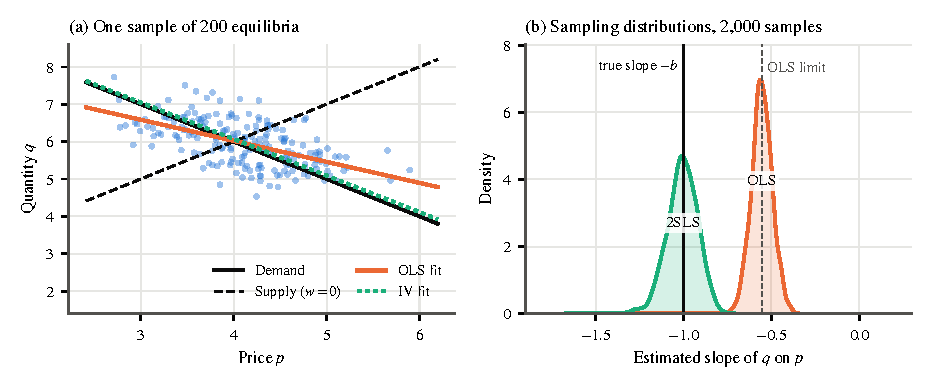
\includegraphics[width=\textwidth]{figures/appA/simultaneity.pdf}
\caption{Simultaneity bias and instrumental variables in a simulated market. Demand is
$q_t = 10 - p_t + u^d_t$ and supply is $q_t = 2 + p_t + w_t + u^s_t$, with $w_t \sim N(0, 1)$,
$u^d_t \sim N(0, 0.36)$ and $u^s_t \sim N(0, 0.25)$, all independent. (a) One sample of 200 equilibria with the
true demand curve and the supply curve at $w_t = 0$. The OLS fit has slope $-0.563$, and the IV fit with
instrument $w_t$ has slope $-0.977$. (b) Kernel densities of the OLS and two-stage least squares (2SLS, \cref{sec:A-2sls}) slopes over 2,000 samples of 200
markets. The solid line marks the demand slope $-1$ and the dashed line the OLS limit $-0.553$ from
\cref{prop:A-ols-simultaneity}. The mean first-stage $F$ statistic (\cref{sec:A-weakiv}) is 331. Seed 20261022, script
\texttt{sim\_iv.py}.}
\label{fig:A-simultaneity}
\end{figure}

\casehead{Order and rank conditions}
\Cref{cor:A-shifter} extends to any linear system. Let $y_t$ be a $G \times 1$ vector of endogenous variables
and $x_t$ an $M \times 1$ vector of exogenous variables with $\E[x_t x_t^\top]$ nonsingular. The structural
system is $B y_t + \Gamma x_t = u_t$, with $B$ nonsingular and $\E[x_t u_t^\top] = 0$. Its reduced form is
\begin{equation}\label{eq:A-system-rf}
y_t = \Pi x_t + v_t, \qquad \Pi = -B^{-1}\Gamma, \qquad v_t = B^{-1}u_t .
\end{equation}
The reduced-form coefficients are identified, $\Pi = \E[y_t x_t^\top]\E[x_t x_t^\top]^{-1}$, because $v_t$ is
uncorrelated with $x_t$. Consider one structural equation, normalized on its first endogenous variable:
\begin{equation}\label{eq:A-struct-eq}
y_{1t} = Y_{1t}^\top\beta + X_{1t}^\top\gamma + u_{1t} .
\end{equation}
It includes $G_1$ further endogenous variables $Y_{1t}$ and $M_1$ exogenous variables $X_{1t}$. The remaining
$M_2 = M - M_1$ exogenous variables $X_{2t}$ are excluded. Partition the reduced form conformably,
\begin{equation*}
y_{1t} = \pi_{11}^\top X_{1t} + \pi_{12}^\top X_{2t} + v_{1t}, \qquad
Y_{1t} = \Pi_{21}X_{1t} + \Pi_{22}X_{2t} + V_{1t},
\end{equation*}
where $\Pi_{22}$ is $G_1 \times M_2$. Substitute both into \eqref{eq:A-struct-eq}. The resulting identity holds
for all values of the exogenous variables, and the reduced-form errors are uncorrelated with them. Hence the
coefficients on $X_{1t}$ and $X_{2t}$ must match:
\begin{equation}\label{eq:A-rf-restrictions}
\pi_{11} = \Pi_{21}^\top\beta + \gamma, \qquad \pi_{12} = \Pi_{22}^\top\beta .
\end{equation}

\begin{proposition}[Rank and order conditions]\label{prop:A-rank}
The coefficients $(\beta, \gamma)$ of \eqref{eq:A-struct-eq} are identified if and only if
$\mathrm{rank}(\Pi_{22}) = G_1$. A necessary condition is $M_2 \ge G_1$, so the equation must exclude at least
as many exogenous variables as it includes endogenous variables on its right-hand side.
\end{proposition}

\begin{proof}
The second block of \eqref{eq:A-rf-restrictions} is a system of $M_2$ linear equations in the $G_1$ unknowns
$\beta$. If $\Pi_{22}^\top$ has full column rank $G_1$, the solution is unique:
\begin{equation*}
\beta = (\Pi_{22}\Pi_{22}^\top)^{-1}\Pi_{22}\,\pi_{12}, \qquad \gamma = \pi_{11} - \Pi_{21}^\top\beta .
\end{equation*}
If the rank is below $G_1$, pick $h \neq 0$ with $\Pi_{22}^\top h = 0$. The pair
$(\beta + h, \gamma - \Pi_{21}^\top h)$ also satisfies \eqref{eq:A-rf-restrictions}. The error it implies is
\begin{align*}
y_{1t} - Y_{1t}^\top(\beta + h) - X_{1t}^\top(\gamma - \Pi_{21}^\top h)
&= u_{1t} - h^\top\bigl(\Pi_{21}X_{1t} + \Pi_{22}X_{2t} + V_{1t}\bigr) + h^\top\Pi_{21}X_{1t} \\
&= u_{1t} - h^\top V_{1t} ,
\end{align*}
which is uncorrelated with $x_t$. The two coefficient vectors fit the same observables and satisfy the same
exogeneity restrictions, so the data cannot distinguish them. The order condition follows from
$\mathrm{rank}(\Pi_{22}) \le M_2$.
\end{proof}

In the market of \cref{cor:A-shifter}, demand includes one endogenous regressor (price) and excludes one
exogenous variable ($w_t$). The relevant reduced-form coefficient is $\Pi_{22} = -\frac{\delta}{b + c}$, which
is nonzero when $\delta \neq 0$, so demand is exactly identified. Supply excludes nothing, $M_2 = 0 < 1$, and
its slope remains unidentified until we observe a demand shifter.

\casehead{The link to conduct}
The same algebra explains why conduct is hard to identify (\cref{sec:03-identification}). In the linear model
of \cref{eq:03-linear-system}, the supply relation is $P_t = b_0 + \lambda Q_t + b_2 W_t + u^s_t$ with composite
slope $\lambda = b_1 - \frac{\theta}{a_1}$, where $\theta$ is conduct. An excluded demand shifter identifies
$\lambda$ by \cref{prop:A-rank}. The slope of marginal cost $b_1$ and conduct $\theta$ enter only through
$\lambda$. The Jacobian of the map from $(b_1, \theta)$ to the identified coefficients therefore has rank one,
and the two are not separately identified (\cref{prop:03-obs-equiv}). A demand rotator, a variable that changes
the slope of demand, makes the markup term move independently of quantity and restores identification
\citep{Bresnahan1982,Lau1982}. \Cref{sec:03-rotation} develops the argument.

\subsection{Potential outcomes and selection}\label{sec:A-potential}

Many questions in the book ask what an intervention does: a merger, a tax, entry by a rival. The
\emph{potential outcomes} framework states such questions precisely. Let $d_i \in \{0, 1\}$ indicate
treatment of unit $i$. The unit has two potential outcomes, $y_i(1)$ if treated and $y_i(0)$ if not, and we
observe only $y_i = d_i\,y_i(1) + (1 - d_i)\,y_i(0)$. The \emph{average treatment effect} is
$\mathrm{ATE} = \E[y_i(1) - y_i(0)]$, and the \emph{average treatment effect on the treated} is
$\mathrm{ATT} = \E[y_i(1) - y_i(0) \mid d_i = 1]$.

\begin{proposition}[Selection bias]\label{prop:A-selection}
The difference in mean outcomes between treated and untreated units satisfies
\begin{equation}\label{eq:A-selection}
\E[y_i \mid d_i = 1] - \E[y_i \mid d_i = 0]
= \mathrm{ATT} + \bigl\{\E[y_i(0) \mid d_i = 1] - \E[y_i(0) \mid d_i = 0]\bigr\} .
\end{equation}
\end{proposition}

\begin{proof}
Observed outcomes equal the relevant potential outcomes, so $\E[y_i \mid d_i = 1] = \E[y_i(1) \mid d_i = 1]$
and $\E[y_i \mid d_i = 0] = \E[y_i(0) \mid d_i = 0]$. Add and subtract $\E[y_i(0) \mid d_i = 1]$:
\begin{equation*}
\E[y_i(1) \mid d_i = 1] - \E[y_i(0) \mid d_i = 1] + \E[y_i(0) \mid d_i = 1] - \E[y_i(0) \mid d_i = 0] .
\end{equation*}
The first two terms form the ATT and the last two the bracket in \eqref{eq:A-selection}.
\end{proof}

The bracket is the \emph{selection bias}. It compares the untreated outcomes of two different groups, and it
is nonzero whenever the treated would have fared differently even without treatment. Random assignment makes
$d_i$ independent of $(y_i(1), y_i(0))$. The selection term then vanishes, and the ATT equals the ATE.

Selection is the central problem of merger retrospectives. Merging firms differ from non-merging ones, and
so do the rivals of merging firms. In hospital markets, non-merging hospitals whose rivals later merged had
price growth of $-2.9$ percent in 1985--1988, against $4.2$ percent for hospitals without merging rivals
\citep[p.~16]{Dafny2005}. A naive comparison would attribute part of this pre-existing gap to the mergers.
\Cref{sec:A-ivmodel} shows how an instrument removes it.

The same decomposition applies to continuous treatments. In the cross-industry regressions of the
structure-conduct-performance (SCP) paradigm, industry $k$ has a potential Lerner index $L_k(h)$ at each concentration level
$h$, and we observe $L_k = L_k(\HHI_k)$. Comparing industries at $h$ and $h'$,
\begin{multline*}
\E[L_k \mid \HHI_k = h] - \E[L_k \mid \HHI_k = h'] = \E[L_k(h) - L_k(h') \mid \HHI_k = h] \\
+ \bigl\{\E[L_k(h') \mid \HHI_k = h] - \E[L_k(h') \mid \HHI_k = h']\bigr\} .
\end{multline*}
The first term is a causal effect and the second a selection term, as in \cref{eq:01-potential-outcomes}.
Concentration is an equilibrium outcome of the same demand and cost primitives that determine margins, so
the selection term has no reason to vanish (\cref{sec:01-endogeneity}).

\casehead{Three empirical strategies on one industry}
The airline studies of \cref{ch:airlines} show three ways to overcome selection, each with its own
identifying assumption. \citet{Borenstein1989} runs reduced-form fare regressions on a carrier's route and
airport shares. His route-share effect is identified by an instrument, the carrier's share of endpoint
enplanements. He excludes it on the ground that fares respond to actual competition only
(\cref{sec:A-ivsources}). \citet{WhinstonCollins1992} run an event study of entry announcements. The value
effect of entry on incumbents is identified by the timing of news under efficient stock markets
(\cref{sec:A-eventstudy}). \citet{BerryCarnallSpiller2006} estimate a structural model of demand and
pricing.\footnote{We read NBER Working Paper 5561 (1996), \citet{BerryCarnallSpiller1996}, an earlier version of
their chapter. Page and table numbers marked WP refer to it.} Markups are identified by the estimated demand system together with an equilibrium assumption on
pricing. The three designs answer different questions, and their assumptions fail in different ways. A
related distinction is between prospective analysis, which predicts the effect of a change before it
happens, and retrospective analysis, which measures it afterwards (\cref{ch:mergers}). \Cref{sec:A-did}
develops the designs behind retrospectives.

\casehead{Partial identification}
When the assumptions needed for point identification are not credible, weaker assumptions often still bound
the feature of interest. \citet{HaileTamer2003} study English auctions in which bids need not equal values.
They assume only that bidders never bid more than their values and never let an opponent win at a price they
would have been willing to beat. These two inequalities bound the distribution of values from above and below.
\citet[pp.~493--499]{AradillasLopezGandhiQuint2013} allow symmetric private values with nonnegative dependence
when only the transaction price and the number of bidders are observed. The distribution of the highest value is then only partially
identified. If values are independent of the number of bidders, variation in that number across auctions tightens
the bounds on the seller's expected profit, the bidders' surplus and the optimal reserve price.
\Cref{ch:auction-empirics} develops both results, and \cref{sec:A-partialid} treats estimation and inference
for bounds.

\subsection{Monte Carlo experiments}\label{sec:A-montecarlo}

A \emph{Monte Carlo experiment} studies an estimator by applying it to data simulated from a known
data-generating process. It proceeds in four steps.
\begin{enumerate}[label=(\arabic*)]
\item Specify the data-generating process completely: functional forms, the true parameter $\theta_0$, the
  distributions of exogenous variables and errors, and the sample size $n$.
\item Fix the seed of the random number generator, so that the experiment can be reproduced exactly.
\item For $r = 1, \dots, R$, draw a sample and compute the estimate $\hat\theta_r$, its standard error and
  any test decision $D_r \in \{0, 1\}$, which equals one if the test rejects.
\item Summarize the $R$ replications.
\end{enumerate}
For a scalar parameter the usual summaries are the bias $\bar\theta - \theta_0$ with
$\bar\theta = \frac{1}{R}\sum_r\hat\theta_r$ and the standard deviation of $\hat\theta_r$ across replications.
Others are the \emph{root mean squared error}
$\mathrm{RMSE} = \bigl[\frac{1}{R}\sum_r(\hat\theta_r - \theta_0)^2\bigr]^{\frac{1}{2}}$, the coverage rate of
nominal confidence intervals, and the rejection rate $\frac{1}{R}\sum_r D_r$ of a test. Adding and
subtracting $\bar\theta$ inside the square gives
\begin{equation*}
\frac{1}{R}\sum_{r=1}^{R}(\hat\theta_r - \theta_0)^2
= (\bar\theta - \theta_0)^2 + \frac{1}{R}\sum_{r=1}^{R}(\hat\theta_r - \bar\theta)^2 ,
\end{equation*}
because the cross term $\frac{2}{R}(\bar\theta - \theta_0)\sum_r(\hat\theta_r - \bar\theta)$ is zero. The
squared RMSE is the squared bias plus the variance. Some estimators have no finite mean, such as
just-identified two-stage least squares (\cref{sec:A-weakiv}). For them the median and interquantile ranges
are more informative than the mean and the RMSE.

Monte Carlo summaries are estimates with their own sampling error. Consider a test whose true rejection
probability is $\alpha$. The replications are independent, so $\sum_r D_r$ is binomial with $R$ trials and
success probability $\alpha$. The estimated rejection rate $\hat\alpha = \frac{1}{R}\sum_r D_r$ therefore
satisfies
\begin{equation}\label{eq:A-mc-se}
\E[\hat\alpha] = \alpha, \qquad
\Var(\hat\alpha) = \frac{1}{R^2}\,R\,\alpha(1 - \alpha) = \frac{\alpha(1 - \alpha)}{R}, \qquad
\mathrm{se}(\hat\alpha) = \sqrt{\frac{\alpha(1 - \alpha)}{R}} .
\end{equation}
With $R = 10{,}000$ and $\alpha = 0.05$ the Monte Carlo standard error is 0.0022. A rejection rate of 0.058
then differs from 0.05 by more than three standard errors. In the same way, the Monte Carlo standard error
of $\bar\theta$ is the standard deviation across replications divided by $\sqrt{R}$.

The book uses such experiments to study SCP regressions on simulated Cournot industries
(\cref{sec:01-montecarlo}) and estimators of random-coefficient demand on simulated markets
(\cref{ch:blp,app:problems}). This appendix uses them throughout. They study instrumental variables
(\cref{fig:A-simultaneity,fig:A-weakiv}), latent regimes (\cref{fig:A-em}) and simulation estimators
(\cref{fig:A-simest}). They also study clustered inference (\cref{fig:A-cluster-mc}), kernel estimators
(\cref{fig:A-kde,fig:A-gpv}) and staggered difference in differences (\cref{fig:A-staggered}). Every one of
them reports its seed and the script that produced it.

\section{Least squares, panel data and systems}\label{sec:A-ols}

Ordinary least squares is the workhorse of empirical work, and it reappears inside almost every estimator
in the book. This section treats it as a projection, derives its large-sample behavior, lists the three
classic sources of bias, and develops the panel and system extensions used in the chapters.

\subsection{OLS as a projection}\label{sec:A-projection}

Let $(y_i, x_i)$ be independent and identically distributed, with $\E[y_i^2]$ finite and
$\E[x_i x_i^\top]$ finite and nonsingular. The \emph{linear projection} of $y_i$ on $x_i$ has coefficient
\begin{equation}\label{eq:A-projection}
\beta = \argmin_{b}\ \E\bigl[(y_i - x_i^\top b)^2\bigr] = \E[x_i x_i^\top]^{-1}\E[x_i y_i] .
\end{equation}
The second equality solves the first-order condition $\E[x_i(y_i - x_i^\top\beta)] = 0$. The
\emph{projection error} $e_i = y_i - x_i^\top\beta$ satisfies $\E[x_i e_i] = 0$ by construction. The
projection exists whether or not any economic model holds. A structural interpretation of $\beta$ is an
assumption: that the error of the economic model is uncorrelated with $x_i$, so the structural coefficient
coincides with the projection coefficient.

In a sample of size $n$, stack the observations into $y$ ($n \times 1$) and $X$ ($n \times K$) with full
column rank. The OLS estimator $\hat\beta = (X^\top X)^{-1}X^\top y$ solves the \emph{normal equations}
$X^\top(y - X\hat\beta) = 0$. Define the projection matrix $P_X = X(X^\top X)^{-1}X^\top$ and the
\emph{annihilator} $M_X = I_n - P_X$. Both are symmetric and idempotent, $M_X X = 0$, fitted values are
$P_X y$ and residuals are $\hat e = M_X y$.

\begin{theorem}[Frisch-Waugh-Lovell]\label{thm:A-fwl}
Partition $X = [X_1, X_2]$ and $\hat\beta = (\hat\beta_1^\top, \hat\beta_2^\top)^\top$ conformably, and let
$M_{X_2} = I_n - X_2(X_2^\top X_2)^{-1}X_2^\top$. Then
\begin{equation}\label{eq:A-fwl}
\hat\beta_1 = (X_1^\top M_{X_2} X_1)^{-1}X_1^\top M_{X_2} y = (\tilde X_1^\top\tilde X_1)^{-1}\tilde X_1^\top\tilde y,
\qquad \tilde X_1 = M_{X_2}X_1,\ \tilde y = M_{X_2} y ,
\end{equation}
and the residuals of the regression of $\tilde y$ on $\tilde X_1$ equal the residuals of the full regression.
\end{theorem}

\begin{proof}
The normal equations of the full regression are
\begin{equation*}
X_1^\top(y - X_1\hat\beta_1 - X_2\hat\beta_2) = 0, \qquad X_2^\top(y - X_1\hat\beta_1 - X_2\hat\beta_2) = 0 .
\end{equation*}
The second block gives $\hat\beta_2 = (X_2^\top X_2)^{-1}X_2^\top(y - X_1\hat\beta_1)$. Substituting,
\begin{equation*}
y - X_1\hat\beta_1 - X_2\hat\beta_2 = M_{X_2}(y - X_1\hat\beta_1) .
\end{equation*}
The first block becomes $X_1^\top M_{X_2}(y - X_1\hat\beta_1) = 0$, so
$\hat\beta_1 = (X_1^\top M_{X_2}X_1)^{-1}X_1^\top M_{X_2}y$. The inverse exists because $X$ has full column rank.
Since $M_{X_2}$ is symmetric and idempotent, $X_1^\top M_{X_2}X_1 = \tilde X_1^\top\tilde X_1$ and
$X_1^\top M_{X_2}y = \tilde X_1^\top\tilde y$. The full residual is $M_{X_2}(y - X_1\hat\beta_1) = \tilde y -
\tilde X_1\hat\beta_1$, which is the residual of the partialled regression.
\end{proof}

The theorem says that the coefficient on $X_1$ uses only the variation in $X_1$ that $X_2$ cannot explain.
The theorem underlies fixed effects (\cref{sec:A-panel}) and the control-function form of two-stage
least squares (\cref{sec:A-2sls}). It also justifies partialling out exogenous regressors
(\cref{sec:A-weakiv}) and concentrating out linear parameters (\cref{sec:A-gmm-computation}). The
double-residual estimator of the partially linear model (\cref{sec:A-plm}), the two-way fixed-effects
regression (\cref{sec:A-did-twfe}) and event-study dummies (\cref{sec:A-es-regression}) rest on it as well.

\subsection{Large-sample theory}\label{sec:A-ols-asy}

\begin{assumption}[Linear regression]\label{ass:A-ols}
\leavevmode
\begin{enumerate}[label=(\roman*)]
\item The observations $(y_i, x_i)$ are independent and identically distributed.
\item $y_i = x_i^\top\beta + e_i$ with $\E[x_i e_i] = 0$.
\item $Q = \E[x_i x_i^\top]$ is finite and nonsingular.
\item $\E\lVert x_i\rVert^4 < \infty$ and $\E[e_i^4] < \infty$.
\end{enumerate}
\end{assumption}

Part (iv) guarantees, by the Cauchy-Schwarz inequality, that $\Omega = \E[e_i^2x_ix_i^\top]$ is finite.

\begin{proposition}[Consistency and asymptotic normality of OLS]\label{prop:A-ols-asy}
Under \cref{ass:A-ols}, $\hat\beta \xrightarrow{p} \beta$ and
\begin{equation}\label{eq:A-ols-sandwich}
\sqrt{n}(\hat\beta - \beta) \xrightarrow{d} N\bigl(0,\ Q^{-1}\Omega Q^{-1}\bigr) .
\end{equation}
\end{proposition}

\begin{proof}
Substitute $y = X\beta + e$ into the estimator:
\begin{equation*}
\hat\beta - \beta = \Bigl(\frac{1}{n}X^\top X\Bigr)^{-1}\frac{1}{n}X^\top e
= \Bigl(\frac{1}{n}\sum_{i=1}^n x_ix_i^\top\Bigr)^{-1}\frac{1}{n}\sum_{i=1}^n x_ie_i .
\end{equation*}
By the weak law of large numbers, $\frac{1}{n}\sum_i x_ix_i^\top \xrightarrow{p} Q$ and
$\frac{1}{n}\sum_i x_ie_i \xrightarrow{p} \E[x_ie_i] = 0$. Matrix inversion is continuous at the nonsingular
$Q$, so the continuous mapping theorem gives $\hat\beta - \beta \xrightarrow{p} Q^{-1}\cdot 0 = 0$. For the
distribution, multiply by $\sqrt{n}$:
\begin{equation*}
\sqrt{n}(\hat\beta - \beta) = \Bigl(\frac{1}{n}\sum_{i=1}^n x_ix_i^\top\Bigr)^{-1}
\frac{1}{\sqrt{n}}\sum_{i=1}^n x_ie_i .
\end{equation*}
The terms $x_ie_i$ are independent with mean zero and finite variance $\Omega$, so the central limit theorem
gives $\frac{1}{\sqrt{n}}\sum_i x_ie_i \xrightarrow{d} N(0, \Omega)$. By Slutsky's theorem the product
converges to $Q^{-1}N(0, \Omega) = N(0, Q^{-1}\Omega Q^{-1})$.
\end{proof}

The variance in \eqref{eq:A-ols-sandwich} is called a \emph{sandwich} because $\Omega$ sits between two
copies of $Q^{-1}$. Under \emph{homoskedasticity}, $\E[e_i^2 \mid x_i] = \sigma^2$, the middle term becomes
$\Omega = \sigma^2Q$ and the variance collapses to $\sigma^2Q^{-1}$. Its conventional estimator is
$s^2(X^\top X)^{-1}$ with $s^2 = \frac{\hat e^\top\hat e}{n - K}$. Without homoskedasticity,
\citet{White1980} shows that
\begin{equation}\label{eq:A-hc0}
\hat V_{\mathrm{HC0}} = (X^\top X)^{-1}\Bigl(\sum_{i=1}^n\hat e_i^2x_ix_i^\top\Bigr)(X^\top X)^{-1}
\end{equation}
consistently estimates the variance of $\hat\beta$, in the sense that $n\hat V_{\mathrm{HC0}}
\xrightarrow{p} Q^{-1}\Omega Q^{-1}$. Finite-sample versions adjust the squared residuals, which are too
small on average. Let $h_{ii} = x_i^\top(X^\top X)^{-1}x_i$ be the \emph{leverage} of observation $i$. Under
homoskedasticity, $\hat e = M_Xe$ implies
\begin{equation*}
\E[\hat e_i^2 \mid X] = \sigma^2(M_X)_{ii} = \sigma^2(1 - h_{ii}) .
\end{equation*}
HC1 multiplies \eqref{eq:A-hc0} by $\frac{n}{n - K}$. HC2 replaces $\hat e_i^2$ by $\frac{\hat e_i^2}{1 - h_{ii}}$,
which is unbiased under homoskedasticity. HC3 uses $\frac{\hat e_i^2}{(1 - h_{ii})^2}$, which approximates the
jackknife and is conservative in small samples \citep{MacKinnonWhite1985}. In this book ``robust'' standard
errors mean heteroskedasticity-robust standard errors. They still assume independence across observations.
Clustered and serially correlated data need the estimators of \cref{sec:A-se}, which also covers heteroskedasticity
and autocorrelation consistent (HAC) estimators.

\subsection{Three sources of bias}\label{sec:A-bias}

OLS converges to the projection coefficient. It is biased for the structural coefficient whenever the
structural error is correlated with the regressors. Three mechanisms produce that correlation.

\casehead{Omitted variables}
Suppose $y_i = \beta_0 + \beta_1x_{1i} + \beta_2x_{2i} + e_i$ with $\E[e_i] = 0$ and $e_i$ uncorrelated with
both regressors, but we regress $y_i$ on a constant and $x_{1i}$ only. The short slope converges to
\begin{equation}\label{eq:A-ovb}
\frac{\Cov(y_i, x_{1i})}{\Var(x_{1i})}
= \frac{\beta_1\Var(x_{1i}) + \beta_2\Cov(x_{2i}, x_{1i}) + \Cov(e_i, x_{1i})}{\Var(x_{1i})}
= \beta_1 + \beta_2\,\frac{\Cov(x_{1i}, x_{2i})}{\Var(x_{1i})} .
\end{equation}
The bias is the effect of the omitted variable times the slope of its projection on the included one. With
vector regressors the bias is $\E[x_1x_1^\top]^{-1}\E[x_1x_2^\top]\beta_2$. In the firm-level regressions
that pit industry concentration against firm market share, omitting the share loads its effect onto
concentration whenever the two are correlated (\cref{sec:01-demsetz}).

\casehead{Measurement error}
Suppose $y_i = \beta_0 + \beta x_i^* + e_i$, but we observe $x_i = x_i^* + m_i$. The \emph{classical}
measurement error $m_i$ has mean zero and variance $\sigma_m^2$ and is uncorrelated with $x_i^*$ and $e_i$.
The OLS slope of $y_i$ on $x_i$ converges to
\begin{equation}\label{eq:A-attenuation}
\frac{\Cov(\beta_0 + \beta x_i^* + e_i,\ x_i^* + m_i)}{\Var(x_i^* + m_i)}
= \frac{\beta\Var(x_i^*)}{\Var(x_i^*) + \sigma_m^2} \equiv \beta\lambda .
\end{equation}
The \emph{reliability ratio} $\lambda \in (0, 1]$ is the share of the variance of the measured regressor that
is signal, so the slope is biased toward zero. Panel data with fixed effects can make this
\emph{attenuation} much worse \citep{GrilichesHausman1986}.

\begin{proposition}[Attenuation with fixed effects]\label{prop:A-fe-attenuation}
Let $y_{it} = \alpha_i + \beta x_{it}^* + e_{it}$ for $i = 1, \dots, n$ and $t = 1, \dots, T$, with $T$ fixed,
units independent, and $\E[e_{it} \mid x_{i1}^*, \dots, x_{iT}^*, \alpha_i] = 0$. We observe
$x_{it} = x_{it}^* + m_{it}$, where $m_{it}$ is independent across $i$ and $t$, has mean zero and variance
$\sigma_m^2$, and is independent of $\{x_{is}^*\}$, $\{e_{is}\}$ and $\alpha_i$. Define the within variance
$\Var_W(z) = \E\bigl[\frac{1}{T}\sum_t(z_{it} - \bar z_i)^2\bigr]$ with $\bar z_i = \frac{1}{T}\sum_t z_{it}$,
and suppose $\Var_W(x^*) > 0$. As $n \to \infty$ the within estimator converges to
\begin{equation}\label{eq:A-fe-attenuation}
\beta\lambda_W, \qquad
\lambda_W = \frac{\Var_W(x^*)}{\Var_W(x^*) + \frac{T - 1}{T}\sigma_m^2} .
\end{equation}
\end{proposition}

\begin{proof}
Write $\ddot z_{it} = z_{it} - \bar z_i$. The within transformation removes $\alpha_i$, so
$\ddot y_{it} = \beta\ddot x_{it}^* + \ddot e_{it}$, and the measured regressor is
$\ddot x_{it} = \ddot x_{it}^* + \ddot m_{it}$. The within estimator is
$\frac{\sum_i\sum_t\ddot x_{it}\ddot y_{it}}{\sum_i\sum_t\ddot x_{it}^2}$. Divide numerator and denominator by
$nT$ and apply the law of large numbers across units. The numerator converges to
$\beta\Var_W(x^*)$. The cross terms vanish because $m$ is independent of $x^*$ and $e$, and because strict
exogeneity makes $\E[\ddot x_{it}^*\ddot e_{it}] = 0$. The denominator converges to
$\Var_W(x^*) + \E\bigl[\frac{1}{T}\sum_t\ddot m_{it}^2\bigr]$. For each $t$,
\begin{equation*}
\E[\ddot m_{it}^2] = \Var(m_{it}) - 2\Cov(m_{it}, \bar m_i) + \Var(\bar m_i)
= \sigma_m^2 - \frac{2\sigma_m^2}{T} + \frac{\sigma_m^2}{T} = \frac{T - 1}{T}\,\sigma_m^2 .
\end{equation*}
The ratio of the two limits is \eqref{eq:A-fe-attenuation}.
\end{proof}

Compare $\lambda_W$ with the reliability ratio $\lambda = \frac{\Var(x^*)}{\Var(x^*) + \sigma_m^2}$ of a pooled
regression, which is valid if $\alpha_i$ is unrelated to the regressor. Inverting both ratios shows that
$\lambda_W < \lambda$ if and only if
\begin{equation*}
\frac{\Var_W(x^*)}{\Var(x^*)} < \frac{T - 1}{T} .
\end{equation*}
The left side is the share of the signal's variance that occurs within units. The right side is the same
share for independent noise. A persistent signal, whose variance is mostly between units, satisfies the
inequality easily. For example, if $x_{it}^* = a_i + \xi_{it}$ with independent $\xi_{it}$ of variance
$\sigma_\xi^2$ and $\Var(a_i) = \sigma_a^2$, then $\Var_W(x^*) = \frac{T - 1}{T}\sigma_\xi^2$ and
$\lambda_W = \frac{\sigma_\xi^2}{\sigma_\xi^2 + \sigma_m^2}$. This falls short of $\lambda$ whenever
$\sigma_a^2 > 0$. The result is the formal content of the critique that panel regressions of margins on
concentration with industry effects \citep{Salinger1990} can worsen attenuation
(\cref{prop:01-fe-attenuation}).

\casehead{Simultaneity}
\Cref{prop:A-ols-simultaneity} is the third mechanism. When the regressor is an equilibrium outcome, the
error of each equation moves it. Invalid instruments can bring the same bias back. With national demand
shocks, prices of the same brand in other cities are correlated with local demand errors. An instrumental
variables estimator built on them then ``is like doing ordinary least squares on a supply and demand
system'' \citep[p.~242]{Bresnahan1997}. \Cref{sec:A-ivmodel} gives the general formula, and
\cref{sec:10-bresnahan-iv} works out the cereal case.

\casehead{The structure-conduct-performance regression as a projection}
These mechanisms combine in the cross-industry regression of margins on concentration. Its OLS slope
converges to $\frac{\Cov(L_k, \HHI_k)}{\Var(\HHI_k)}$, a projection coefficient. Suppose every industry is a
symmetric Cournot industry, so $L_k = \frac{\HHI_k}{\varepsilon_k}$. If the elasticity $\varepsilon_k$ is
independent of $\HHI_k$, then $\Cov(L_k, \HHI_k) = \E[\frac{1}{\varepsilon_k}]\Var(\HHI_k)$, and the slope
converges to $\E[\frac{1}{\varepsilon_k}]$. Once elasticities, entry costs and conduct vary with
concentration, the slope mixes comparative statics with respect to several primitives and has no structural
meaning (\cref{prop:01-scp-plim}).

\subsection{Panel data}\label{sec:A-panel}

A \emph{panel} observes units $i = 1, \dots, n$ over periods $t = 1, \dots, T$. The basic model is
\begin{equation}\label{eq:A-panel}
y_{it} = x_{it}^\top\beta + \alpha_i + e_{it} ,
\end{equation}
where the unit effect $\alpha_i$ may be correlated with the regressors in any way. The key assumption is
\emph{strict exogeneity}, $\E[e_{it} \mid x_{i1}, \dots, x_{iT}, \alpha_i] = 0$: shocks in any period are
unrelated to the regressors in every period.

\casehead{Fixed effects}
Stack the data unit by unit and write $D = I_n \otimes \iota_T$ for the $nT \times n$ matrix of unit dummies,
where $\iota_T$ is a $T \times 1$ vector of ones. The \emph{fixed-effects}, or \emph{within}, estimator is OLS
of $y$ on $X$ and $D$. By \cref{thm:A-fwl} it equals OLS after premultiplying by
\begin{equation*}
M_D = I_{nT} - D(D^\top D)^{-1}D^\top = I_n \otimes \Bigl(I_T - \frac{1}{T}\iota_T\iota_T^\top\Bigr) ,
\end{equation*}
which subtracts each unit's time mean. Hence $\hat\beta_W = \bigl(\sum_i\sum_t\ddot x_{it}\ddot x_{it}^\top\bigr)^{-1}
\sum_i\sum_t\ddot x_{it}\ddot y_{it}$ with $\ddot z_{it} = z_{it} - \bar z_i$. It is consistent as $n \to \infty$
with $T$ fixed under strict exogeneity. Regressors that do not vary over time are swept out, and the error
variance is estimated with $nT - n - K$ degrees of freedom.

\casehead{First differences}
Differencing \eqref{eq:A-panel} also removes $\alpha_i$: $\Delta y_{it} = \Delta x_{it}^\top\beta + \Delta e_{it}$
for $t \ge 2$. OLS on the differences is consistent when $\E[\Delta x_{it}\Delta e_{it}] = 0$. With $T = 2$ the two
estimators coincide. The within deviations are $\ddot z_{i1} = -\frac{1}{2}\Delta z_{i2}$ and
$\ddot z_{i2} = \frac{1}{2}\Delta z_{i2}$, so
\begin{equation*}
\hat\beta_W = \Bigl(\sum_i 2\cdot\frac{1}{4}\Delta x_{i2}\Delta x_{i2}^\top\Bigr)^{-1}\sum_i 2\cdot\frac{1}{4}\Delta x_{i2}\Delta y_{i2}
= \Bigl(\sum_i\Delta x_{i2}\Delta x_{i2}^\top\Bigr)^{-1}\sum_i\Delta x_{i2}\Delta y_{i2} ,
\end{equation*}
which is the first-difference estimator. With $T > 2$ they differ, and their relative efficiency depends on
the serial correlation of $e_{it}$.

\casehead{Random effects}
If in addition $\E[\alpha_i \mid x_{i1}, \dots, x_{iT}] = 0$, the unit effect becomes part of a composite error
$\alpha_i + e_{it}$. With $\Var(\alpha_i) = \sigma_\alpha^2$ and homoskedastic, serially uncorrelated $e_{it}$,
the covariance matrix of unit $i$'s errors is $\Omega_i = \sigma_e^2I_T + \sigma_\alpha^2\iota_T\iota_T^\top$.
Write $\bar P = \frac{1}{T}\iota_T\iota_T^\top$ and $\bar Q = I_T - \bar P$. These are orthogonal idempotent
matrices, and
\begin{equation*}
\Omega_i = \sigma_e^2\bar Q + (\sigma_e^2 + T\sigma_\alpha^2)\bar P, \qquad
\sigma_e\,\Omega_i^{-\frac{1}{2}} = \bar Q + \phi\bar P = I_T - (1 - \phi)\bar P, \qquad
\phi = \frac{\sigma_e}{\sqrt{\sigma_e^2 + T\sigma_\alpha^2}} .
\end{equation*}
Generalized least squares is therefore OLS of $y_{it} - \vartheta\bar y_i$ on $x_{it} - \vartheta\bar x_i$ with
$\vartheta = 1 - \phi$. The \emph{random-effects} estimator replaces $\sigma_e^2$ and $\sigma_\alpha^2$ by estimates.
It quasi-demeans: $\vartheta = 0$ gives pooled OLS, and $\vartheta \to 1$ as
$\frac{T\sigma_\alpha^2}{\sigma_e^2} \to \infty$, so random effects approaches fixed effects in long panels
with large unit variance. It is efficient when its assumptions hold and inconsistent when $\alpha_i$ is
correlated with the regressors. \Cref{sec:A-spectests} tests between the two. \citet{FullerBattese1974}
extend the approach to crossed unit and time effects, $\alpha_i + \tau_t + e_{it}$.

\casehead{Two-way fixed effects}
Adding period effects gives $y_{it} = x_{it}^\top\beta + \alpha_i + \tau_t + e_{it}$. In a balanced panel,
\cref{thm:A-fwl} shows that the slope is OLS on the doubly demeaned data
$\ddot z_{it} = z_{it} - \bar z_{i\cdot} - \bar z_{\cdot t} + \bar z_{\cdot\cdot}$, the deviations from unit,
period and grand means. The variation that identifies $\beta$ differs across these estimators. Pooled OLS
uses all variation, including permanent differences across units. Fixed effects uses changes within units
over time. Two-way fixed effects uses changes within units relative to the average change in the same period,
so it is a difference-in-differences design with a continuous treatment (\cref{sec:A-did-twfe}).

\casehead{Application: tax pass-through in cigarettes}
\citet{Sumner1981} estimates the pass-through of state cigarette excise taxes into retail prices. His
equation (4) is $P_{it} = X_{it}\eta + \theta R_{it} + U_{it}$, with $i$ indexing states, $t$ years and
$R_{it}$ the tax per pack. Sumner's $\theta$ is the pass-through rate, which is neither conduct nor a generic
parameter. In the notation of \cref{eq:03-sumner-regression} it is
\begin{equation}\label{eq:A-sumner}
p_{sy} = \mu_s + \tau_y + \rho\,t_{sy} + e_{sy} ,
\end{equation}
with state effects $\mu_s$, year effects $\tau_y$ and pass-through rate $\rho$. The data are annual average
prices and taxes for 1954--1978 in 47 states and the District of Columbia. Alaska, Hawaii and New Hampshire
are excluded, which leaves 1,200 observations (pp.~1016--1017). Sumner's Table 1 reports three estimators of
$\rho$, each with its standard error. Two-way fixed effects by OLS gives 1.074 (0.013). Pooled OLS with the
national consumer price index in place of the year dummies and without state dummies gives 1.029 (0.011). A
variance-components estimator with random state and year effects \citep{FullerBattese1974} and the price index
gives 1.069 (0.013). The $R^2$ is about 0.99 with the dummies and 0.95 without them.

The comparison shows what each estimator uses. The pooled regression compares price levels across states
with permanently different taxes. Sumner notes that the three states with a large stake in tobacco growing
and cigarette manufacturing, North Carolina, Virginia and Kentucky, all have low taxes (fn.~8). State
dummies absorb such stable state characteristics (pp.~1015--1016), and the fixed-effects estimate rests on
changes in taxes within states over time. The random-effects estimate lies close to the fixed-effects one.
This is what quasi-demeaning predicts when $T = 25$ and the state variance component is large relative to
the idiosyncratic variance. The reported standard errors treat the 1,200 observations as independent.
\Cref{sec:A-sumner-se} recomputes them on a reconstructed panel, allowing for serial correlation within states
(\cref{tab:A-sumner}), and \cref{sec:A-did-twfe} reads the regression as a difference in differences with a
continuous treatment. \Cref{sec:03-sumner} discusses the economics of the test.

\subsection{Systems of equations}\label{sec:A-systems}

Many models in the book consist of several equations estimated together. Examples are the share
equations of a demand system, the residual demand curves of several firms, and the returns of several firms
around one event.

\casehead{Seemingly unrelated regressions}
Let $y_g = X_g\beta_g + e_g$ for equations $g = 1, \dots, G$, each with $n$ observations. Stack the equations
as $y = X\beta + e$, with $y = (y_1^\top, \dots, y_G^\top)^\top$ and $X = \diag(X_1, \dots, X_G)$ block diagonal.
Let $e_t = (e_{1t}, \dots, e_{Gt})^\top$ collect the errors of observation $t$, and assume $\E[e_te_t^\top] = \Sigma$
with independence across $t$. Then $\Var(e) = \Sigma \otimes I_n$. Generalized least squares gives the
\emph{seemingly unrelated regressions} (SUR) estimator of \citet{Zellner1962},
\begin{equation}\label{eq:A-sur}
\hat\beta_{SUR} = \bigl[X^\top(\Sigma^{-1}\otimes I_n)X\bigr]^{-1}X^\top(\Sigma^{-1}\otimes I_n)\,y .
\end{equation}
Feasible SUR replaces $\Sigma$ by $\hat\Sigma_{gh} = \frac{1}{n}\hat e_g^\top\hat e_h$ from equation-by-equation OLS
residuals. Iterating between $\hat\Sigma$ and $\hat\beta$ until convergence gives the Gaussian maximum likelihood
estimator.

\begin{proposition}[When SUR equals OLS]\label{prop:A-sur-ols}
If $X_g = X_0$ for every equation, or if $\Sigma$ is diagonal, then \eqref{eq:A-sur} equals equation-by-equation
OLS.
\end{proposition}

\begin{proof}
Use $(A \otimes B)(C \otimes D) = AC \otimes BD$ and $(A \otimes B)^{-1} = A^{-1} \otimes B^{-1}$. With
identical regressors, $X = I_G \otimes X_0$. Then
\begin{align*}
X^\top(\Sigma^{-1}\otimes I_n)X &= (I_G \otimes X_0^\top)(\Sigma^{-1}\otimes I_n)(I_G \otimes X_0)
= \Sigma^{-1}\otimes X_0^\top X_0 ,\\
X^\top(\Sigma^{-1}\otimes I_n)\,y &= (\Sigma^{-1}\otimes X_0^\top)\,y .
\end{align*}
The inverse of the first matrix is $\Sigma \otimes (X_0^\top X_0)^{-1}$, so
\begin{equation*}
\hat\beta_{SUR} = \bigl[\Sigma \otimes (X_0^\top X_0)^{-1}\bigr](\Sigma^{-1}\otimes X_0^\top)\,y
= \bigl[I_G \otimes (X_0^\top X_0)^{-1}X_0^\top\bigr]y ,
\end{equation*}
which stacks the OLS regressions of each $y_g$ on $X_0$. If $\Sigma = \diag(\sigma_1^2, \dots, \sigma_G^2)$,
both $X^\top(\Sigma^{-1}\otimes I_n)X$ and $X^\top(\Sigma^{-1}\otimes I_n)y$ are block diagonal with blocks
$\sigma_g^{-2}X_g^\top X_g$ and $\sigma_g^{-2}X_g^\top y_g$. The weights cancel equation by equation, leaving
$(X_g^\top X_g)^{-1}X_g^\top y_g$.
\end{proof}

SUR gains precision only when the errors are correlated across equations and the regressors differ. It
becomes indispensable when coefficients are restricted across equations. The linear approximate almost ideal demand
system is a leading case of identical regressors. Every share equation contains the same log prices and the same log
total expenditure deflated by the Stone index. Without cross-equation restrictions, OLS equation by equation therefore
coincides with SUR (\cref{sec:05-stone}).

\casehead{Adding up and cross-equation restrictions}
Budget shares sum to one, so the errors of a complete share system sum to zero for every observation, and
$\Sigma$ is singular. We drop one equation and recover its coefficients from the adding-up restrictions. The
maximum likelihood (iterated SUR) estimates do not depend on which equation is dropped \citep{Barten1969}.
Symmetry and homogeneity restrictions take the linear form $R\beta = r$. Restricted GLS minimizes
$(y - Xb)^\top W(y - Xb)$ subject to $Rb = r$, with $W = \Sigma^{-1}\otimes I_n$. The Lagrangian first-order
condition $-2X^\top W(y - Xb) + 2R^\top\ell = 0$ gives $b = \hat\beta - VR^\top\ell$ with
$V = (X^\top WX)^{-1}$. Imposing $Rb = r$ determines the multiplier $\ell$:
\begin{equation}\label{eq:A-restricted-gls}
\tilde\beta = \hat\beta - VR^\top\bigl(RVR^\top\bigr)^{-1}\bigl(R\hat\beta - r\bigr) .
\end{equation}

\casehead{Which restrictions can be tested}
\citet[Section~3.3, pp.~67--70]{DeatonMuellbauer1980b} use the Rotterdam model to sort the restrictions of demand
theory by how they can be tested. For goods $g = 1, \dots, G$ and periods $t$, the model is
\begin{equation}\label{eq:A-rotterdam}
\bar w_{gt}\,\Delta\ln q_{gt} = b_g\,\Delta\ln\bar x_t + \sum_{h=1}^{G}c_{gh}\,\Delta\ln p_{ht} + e_{gt},
\qquad \Delta\ln\bar x_t = \sum_{h=1}^{G}\bar w_{ht}\,\Delta\ln q_{ht}
\end{equation}
(their eqs.~3.3 and~3.4). Here $\bar w_{gt}$ is the budget share used in the discrete approximation to the
differentials. It is chosen so that the identity for $\Delta\ln\bar x_t$ holds in the data (p.~69). The variable
$\Delta\ln\bar x_t$ is the change in real total expenditure, and $b_g$ is the marginal budget share. The coefficient
$c_{gh} = \frac{p_gp_hs_{gh}}{x}$ is a compensated price effect, where $s_{gh}$ is the Slutsky term and $x$ is total
expenditure (their eqs.~3.5 and~3.6). The coefficients are treated as constants. Adding up requires
$\sum_gb_g = 1$ and $\sum_gc_{gh} = 0$ for every $h$ (their eq.~3.7). Homogeneity requires $\sum_hc_{gh} = 0$ for
every $g$, and symmetry requires $c_{gh} = c_{hg}$ (eqs.~3.8 and~3.9). The three restrictions differ in how they
can be tested.

\begin{proposition}[Adding up holds by construction]\label{prop:A-addingup}
Let $y_g = X_0\beta_g + e_g$ for $g = 1, \dots, G$, with common regressors $X_0$ of full column rank. Suppose the
data satisfy $\sum_gy_g = X_0a$ for a known vector $a$. Then the OLS estimates satisfy $\sum_g\hat\beta_g = a$, and
for every observation the OLS residuals sum to zero across equations.
\end{proposition}

\begin{proof}
OLS is linear in the dependent variable, so
\begin{equation*}
\sum_{g=1}^{G}\hat\beta_g = (X_0^\top X_0)^{-1}X_0^\top\sum_{g=1}^{G}y_g = (X_0^\top X_0)^{-1}X_0^\top X_0\,a = a .
\end{equation*}
The residuals then sum to $\sum_gy_g - X_0\sum_g\hat\beta_g = X_0a - X_0a = 0$.
\end{proof}

In \eqref{eq:A-rotterdam} every equation has the same regressors, and the left-hand sides sum to
$\Delta\ln\bar x_t$, the first regressor. The proposition applies with $a$ the first unit vector. OLS therefore
gives $\sum_g\hat b_g = 1$ and $\sum_g\hat c_{gh} = 0$ whatever the data. Adding up cannot be tested, and it places
no restriction on the explanatory power of the equations (p.~69). Homogeneity involves the coefficients of one
equation only. It can be imposed and tested equation by equation, with a $t$ or $F$ test of $\sum_hc_{gh} = 0$.
Symmetry links pairs of equations, so it needs the system, estimated by \eqref{eq:A-restricted-gls} with one
equation dropped. The restrictions are also nested. Under adding up, symmetry gives
$\sum_hc_{gh} = \sum_hc_{hg} = 0$ for every $g$, so symmetry implies homogeneity. Tests of symmetry therefore come
after tests of homogeneity, and \cref{sec:A-wald} reports their outcome. Negativity, the requirement that the matrix
$C = (c_{gh})$ be negative semidefinite, is an inequality restriction and needs other tools.

\Cref{sec:05-estimation} applies these tools to the almost ideal demand system. \citet{Hausman1997}
combines SUR with instruments to estimate brand demand for cereal, a form of three-stage least squares
(\cref{sec:A-3sls,sec:10-hausman-identification}). In event studies with several firms and a common event
date, SUR accounts for the contemporaneous correlation of returns in tests across firms \citep[pp.~172--173]{Binder1985}.
\Citet{WhinstonCollins1992} use it in this way (\cref{sec:A-eventstudy,sec:09-wc}).

\subsection{Testing linear restrictions}\label{sec:A-wald}

Consider $q$ linear restrictions $H_0\colon R\beta = r$, with $R$ a $q \times K$ matrix of rank $q$. Let
$\hat V$ estimate the variance of $\hat\beta$, for example $\frac{1}{n}$ times a consistent estimator of the
asymptotic variance in \eqref{eq:A-ols-sandwich}. The \emph{Wald statistic} is
\begin{equation}\label{eq:A-wald}
\mathcal{W} = (R\hat\beta - r)^\top\bigl[R\hat VR^\top\bigr]^{-1}(R\hat\beta - r) \xrightarrow{d} \chi^2_q
\quad\text{under } H_0 .
\end{equation}
The limit follows in two steps. Under $H_0$, $\sqrt{n}(R\hat\beta - r) = R\sqrt{n}(\hat\beta - \beta)
\xrightarrow{d} N(0, RVR^\top)$ by \cref{prop:A-ols-asy}. If $\zeta \sim N(0, \Sigma_\zeta)$ is $q$-dimensional
with $\Sigma_\zeta$ nonsingular, then $\Sigma_\zeta^{-\frac{1}{2}}\zeta \sim N(0, I_q)$, so
$\zeta^\top\Sigma_\zeta^{-1}\zeta$ is a sum of $q$ squared independent standard normals. Slutsky's theorem
handles the estimated variance. With homoskedastic normal errors and the conventional variance estimator,
$\frac{\mathcal{W}}{q}$ equals
\begin{equation*}
F = \frac{\frac{1}{q}(\mathrm{SSR}_r - \mathrm{SSR}_u)}{\frac{1}{n - K}\mathrm{SSR}_u} \sim F(q, n - K) ,
\end{equation*}
where $\mathrm{SSR}_r$ and $\mathrm{SSR}_u$ are the restricted and unrestricted sums of squared residuals. The
\emph{Chow test} of equal coefficients in two groups is the special case in which the unrestricted model
estimates each group separately \citep{Chow1960a}.

Four applications illustrate the range of uses.
\begin{itemize}
\item \citet{GenesoveMullin1998} test whether the price coefficient and intercept of sugar demand are equal
  across seasons.\footnote{We read the working-paper version of \citet{GenesoveMullin1998}. Equation, table and
  page numbers marked WP refer to it. Printed page numbers are those on the pages of that version.} With
  Newey-West standard errors, the $\chi^2_{(2)}$ statistics are 6.90, 28.18, 29.17 and 25.96 for quadratic,
  linear, log-linear and exponential demand (WP Table~6, p.~29). All exceed the 5 percent cutoff of 5.99, so
  demand rotates between seasons (\cref{tab:03-gm-demand}). A pooled specification with a time trend tests
  instead that the high-season shifts in intercept and slope are both zero. Its statistics are 4.91, 22.73,
  23.40 and 20.77 (WP Table~5, p.~28). The quadratic form does not reject there, so for that form the
  conclusion depends on the specification.
\item The revenue test of \citet{PanzarRosse1987} restricts a single linear combination, the sum
  $\hat\psi = \sum_k\hat\beta_k$ of factor-price elasticities of revenue. With $R = \iota^\top$, the statistic
  is $t = \frac{\hat\psi - \psi_0}{\sqrt{\iota^\top\hat V\iota}}$. Long-run competition implies $\psi = 1$, a
  two-sided test. Monopoly implies $\psi \le 0$, and we reject it at 5 percent when $\frac{\hat\psi}{\mathrm{se}}
  > 1.645$ (\cref{sec:03-panzar-rosse}).
\item \citet[pp.~353--354]{Borenstein1989} rejects a common constant across airlines but fails to reject
  common slopes, so his fare equations pool the slopes and keep carrier effects. A Chow test does not reject
  equal route-share effects across the 20th, 50th and 80th fare percentiles, while it rejects a common
  coefficient on flight frequency (p.~358 and fn.~41). The three percentile regressions use the same routes,
  so a test across them must account for the covariance of their estimates, as a stacked or SUR regression
  does.
\item Tests of demand theory apply the same logic to systems. \citet{Barten1969} estimated the Rotterdam model
  \eqref{eq:A-rotterdam} for 16 groups of Dutch consumption by maximum likelihood, with intercepts for gradual
  changes in tastes. Imposing homogeneity caused ``a very large drop in the value of the maximized likelihood,
  much larger than could conceivably have arisen by chance'' \citep[pp.~69--70]{DeatonMuellbauer1980b}. Symmetry
  was rejected as well, but \citet{Deaton1972} gives technical grounds for doubting that test. \citet{Deaton1974}
  found the same pattern for nine groups of British data from 1900 to 1970. Homogeneity was rejected, while
  symmetry as an additional restriction was not particularly damaging \citep[p.~70]{DeatonMuellbauer1980b}. The
  likelihood ratio statistic used in these studies is asymptotically equivalent to $\mathcal{W}$ under $H_0$
  (\cref{thm:A-trinity}). Each
  rejection is joint, of the theory and of a functional form. Deaton and Muellbauer stress that the Rotterdam,
  double-log and translog systems all reject, at least on aggregate data (pp.~72--74).
\end{itemize}

\section{Instrumental variables}\label{sec:A-iv}

Instrumental variables (IV) are the book's main tool for endogenous regressors: prices in demand equations,
quantities in supply relations, market shares in fare equations and mergers in price regressions. This
section develops the linear model and two-stage least squares, then the special problems of nonlinear models
and weak instruments. It closes with specification tests, heterogeneous effects and system estimation.

\subsection{The IV model}\label{sec:A-ivmodel}

\begin{assumption}[Linear instrumental variables]\label{ass:A-iv}
The observations $(y_i, x_i, z_i)$ are independent and identically distributed, with $x_i$ of dimension $K$
and $z_i$ of dimension $L \ge K$, and
\begin{equation}\label{eq:A-iv-model}
y_i = x_i^\top\beta + e_i .
\end{equation}
\begin{enumerate}[label=(\roman*)]
\item The instruments are exogenous, $\E[z_ie_i] = 0$.
\item The instruments are relevant, $\mathrm{rank}\,\E[z_ix_i^\top] = K$.
\item $\E[z_iz_i^\top]$ is finite and nonsingular, and $\E\lVert z_i\rVert^4$, $\E\lVert x_i\rVert^4$ and $\E[e_i^4]$
  are finite.
\end{enumerate}
\end{assumption}

Exogenous regressors, such as the constant, appear in both $x_i$ and $z_i$. They serve as their own
instruments and are called \emph{included instruments}. The other elements of $z_i$ are the \emph{excluded
instruments}. Exogeneity of an excluded instrument combines two claims. The instrument is unrelated to the
unobserved determinants of the outcome, and it affects the outcome only through $x_i$, which is the
\emph{exclusion restriction}. Relevance requires the excluded instruments to predict every endogenous
regressor beyond what the included instruments predict. In the just-identified case $L = K$, exogeneity gives
$\beta = \E[z_ix_i^\top]^{-1}\E[z_iy_i]$, and the IV estimator is its sample analogue
$\hat\beta_{IV} = (Z^\top X)^{-1}Z^\top y$.

\casehead{Indirect least squares}
Let $y_i = \beta_0 + \beta_1x_i + e_i$ with one instrument $z_i$ and a constant. Exogeneity gives
$\Cov(z_i, y_i) = \beta_1\Cov(z_i, x_i) + \Cov(z_i, e_i) = \beta_1\Cov(z_i, x_i)$, so
\begin{equation}\label{eq:A-ils}
\beta_1 = \frac{\Cov(z_i, y_i)}{\Cov(z_i, x_i)}
= \frac{\frac{\Cov(z_i, y_i)}{\Var(z_i)}}{\frac{\Cov(z_i, x_i)}{\Var(z_i)}} = \frac{\rho_1}{\pi_1} .
\end{equation}
Here $\pi_1$ is the slope of the \emph{first stage}, the regression of $x_i$ on $z_i$. The slope of the
\emph{reduced form}, the regression of $y_i$ on $z_i$, is $\rho_1$. The IV estimand is the reduced-form effect of the
instrument divided by its first-stage effect. The identity also holds exactly in the sample, because each
estimator is a ratio of sample covariances. Estimating $\beta_1$ this way is called \emph{indirect least
squares}. With exogenous controls, \cref{thm:A-fwl} shows that the identity holds after the controls are
partialled out of $y_i$, $x_i$ and $z_i$.

\casehead{The Wald estimator}
If $z_i$ is binary with $p = \Pr(z_i = 1)$, then
\begin{align*}
\Cov(z_i, y_i) &= \E[z_iy_i] - \E[z_i]\E[y_i] \\
&= p\,\E[y_i \mid z_i = 1] - p\bigl(p\,\E[y_i \mid z_i = 1] + (1 - p)\,\E[y_i \mid z_i = 0]\bigr) \\
&= p(1 - p)\bigl(\E[y_i \mid z_i = 1] - \E[y_i \mid z_i = 0]\bigr) .
\end{align*}
The same algebra applies to $x_i$, and \eqref{eq:A-ils} becomes the \emph{Wald estimator}
\begin{equation}\label{eq:A-wald-estimator}
\beta_1 = \frac{\E[y_i \mid z_i = 1] - \E[y_i \mid z_i = 0]}{\E[x_i \mid z_i = 1] - \E[x_i \mid z_i = 0]} .
\end{equation}

\casehead{Invalid instruments}
If the instrument is correlated with the error, the same algebra gives
\begin{equation}\label{eq:A-iv-bias}
\plim\hat\beta_{1,IV} - \beta_1 = \frac{\Cov(z_i, e_i)}{\Cov(z_i, x_i)}
= \frac{\Corr(z_i, e_i)}{\Corr(z_i, x_i)}\cdot\frac{\sigma_e}{\sigma_x} .
\end{equation}
The OLS bias is $\frac{\Cov(x_i, e_i)}{\Var(x_i)} = \Corr(x_i, e_i)\frac{\sigma_e}{\sigma_x}$, so the ratio of the
two biases is
\begin{equation*}
\frac{\plim\hat\beta_{1,IV} - \beta_1}{\plim\hat\beta_{1,OLS} - \beta_1}
= \frac{\Corr(z_i, e_i)}{\Corr(x_i, e_i)\,\Corr(z_i, x_i)} .
\end{equation*}
A weak instrument puts a small $\Corr(z_i, x_i)$ in the denominator. It magnifies even a slight correlation
with the error, and IV can then be more biased than OLS. Weak and slightly invalid instruments are a
dangerous mix. Bresnahan's critique of prices in other cities as instruments is an example. National demand
shocks make $\Cov(z_i, e_i)$ positive, and the larger their share of price variation, the closer the IV bias
comes to the OLS bias (\cref{sec:10-bresnahan-iv}). With a valid and strong instrument, by contrast, 2SLS is
centered on the truth, as panel (b) of \cref{fig:A-simultaneity} shows.

\casehead{Application: rival mergers and hospital prices}
\citet{Dafny2009} estimates the effect of hospital mergers on prices.\footnote{Numbers and page references
follow the NBER working-paper version, revised in October 2007 \citep{Dafny2005}. Table numbers refer to that
version.} A comparison of merging with non-merging hospitals suffers from selection, because hospitals that
merge differ in unobserved ways from those that do not. Following \citet{Eckbo1983}, she studies the
\emph{rivals} of merging hospitals instead. If prices are strategic complements, rivals raise their prices
after a merger as well. Exposure to a rival's merger is still selected, because markets with mergers differ
from markets without them, so she instruments for it.

The data combine 97 independent mergers between 1989 and 1996, in which two hospitals consolidated into a
single licensed entity \citep{DranoveLindrooth2003}, with Medicare cost reports for 1985--2000 (pp.~12--15).
The price of a hospital is its inpatient revenue per case-mix-adjusted non-Medicare discharge. The estimation
sample contains 877 non-merging hospitals with at least two rivals within 7 miles. The treatment $R_i$ is the
number of rival mergers within 7 miles between 1989 and 1996, with mean 0.156 (Table 1). The outcome is price
growth over the merger wave, $\Delta\ln p_i = \ln p_{i,1997} - \ln p_{i,1988}$, with mean 0.010. The instrument
$C_i$ is the number of \emph{co-located} rival pairs, meaning pairs of rivals within 0.3 miles and at most five
blocks of each other in 1988. The estimating equations are
\begin{align}
R_i &= \pi_0 + \pi_1C_i + w_i^\top\pi_2 + v_i && \text{(first stage)}, \label{eq:A-dafny-fs}\\
\Delta\ln p_i &= \rho_0 + \rho_1C_i + w_i^\top\rho_2 + \varepsilon_i && \text{(reduced form)}, \label{eq:A-dafny-rf}\\
\Delta\ln p_i &= \beta_0 + \beta_1R_i + w_i^\top\beta_2 + e_i && \text{(structural equation)}. \label{eq:A-dafny-iv}
\end{align}
The controls $w_i$ include hospital characteristics: ownership, teaching status, Medicaid share,
debt-to-asset ratio, occupancy and bed-size categories. They also include market characteristics, namely
population categories, the penetration of health maintenance organizations and log income per capita, with or
without state fixed effects.

Relevance has an economic rationale. Co-located hospitals can save more by closing duplicate departments,
and they gain more market power from merging, because location is a primary source of differentiation in
inpatient care (p.~3). In the data, co-located hospitals merge at a rate of 11.0 percent, against 3.7 percent
for other hospitals (p.~18). Exclusion requires that rival co-location affect price growth only through rival
mergers. Dafny names the main threat. Before 1988, new hospitals might have entered next to existing ones in
areas where prices were expected to rise. She argues that this is unlikely, because there has been very
little entry into acute care since the Hill-Burton Act of 1946 (fn.~27).

\Cref{tab:A-dafny} reproduces the main results. One more co-located rival pair raises the number of rival
mergers by 0.119, large relative to the mean of 0.156, with a $t$-statistic of about 6.6. It raises price
growth by 0.045, against a mean of 0.010. Because the model is exactly identified, the IV estimate is the ratio
\eqref{eq:A-ils}. The rounded coefficients give $\frac{0.045}{0.119} = 0.378$, and the unrounded ones give the
reported 0.376 (fn.~29). The implied price increase is $e^{0.376} - 1 = 46$ percent, or 35 percent with state
fixed effects (fn.~30). OLS finds no effect, with an estimate of 0.016 and a standard error of 0.026. The sign
of the OLS bias matches the pre-period evidence of \cref{sec:A-potential}. Hospitals later exposed to rival
mergers had lower price growth before the merger wave, so treating rival mergers as exogenous understates
their effect.

\begin{table}[htbp]
\centering
\caption{Rival mergers and hospital price growth: first stage, reduced form, IV and OLS}
\label{tab:A-dafny}
\small
\begin{tabular}{@{}lcc@{}}
\toprule
 & Without state effects & With state effects \\
\midrule
\multicolumn{3}{@{}l}{\textit{A. First stage (OLS)}} \\
Own merger on own co-location ($N = 4{,}487$) & 0.066 & 0.062 \\
 & (0.016) & (0.016) \\
Rival mergers on co-located rival pairs ($N = 877$) & 0.119 & 0.112 \\
 & (0.018) & (0.019) \\
\addlinespace
\multicolumn{3}{@{}l}{\textit{B. Reduced form: log price growth on co-located rival pairs (OLS)}} \\
1985--1988, before the merger wave ($N = 877$) & $-0.016$ & $-0.013$ \\
 & (0.010) & (0.011) \\
1988--1997, merger period ($N = 877$) & 0.045 & 0.034 \\
 & (0.014) & (0.015) \\
1997--2000, after the merger wave ($N = 703$) & $-0.008$ & $-0.001$ \\
 & (0.013) & (0.014) \\
\addlinespace
\multicolumn{3}{@{}l}{\textit{C. Log price growth 1988--1997 on the number of rival mergers ($N = 877$)}} \\
IV, instrument: co-located rival pairs & 0.376 & 0.301 \\
 & (0.132) & (0.147) \\
OLS & 0.016 & $-0.003$ \\
 & (0.026) & (0.027) \\
\bottomrule
\end{tabular}

\smallskip
\begin{minipage}{0.92\textwidth}\footnotesize
Notes: Standard errors in parentheses. Every regression controls for the hospital and market characteristics
listed in the text. The own-merger regression is a linear probability model on all 4,487 hospitals. The other
rows use non-merging hospitals with at least two rivals within 7 miles. Price is inpatient revenue per
case-mix-adjusted non-Medicare discharge, and price changes are censored at the 5th and 95th percentiles.
Source: \citet{Dafny2005}, Table 2 (panel A), Table 3 (panel B) and Table 4 (panel C).
\end{minipage}
\end{table}

Several checks support the design. Rival co-location predicts price growth neither before nor after the
merger wave (panel B), so co-located markets were not on steeper price paths. The IV estimate barely moves
when all controls are dropped, at 0.352 (0.132) (Appendix Table 1). It more than doubles when the market
radius shrinks to 5 miles, at 0.962 (0.377), and it vanishes at 10 miles, at 0.051 (0.054) (Table 5). Effects
that fade with distance are what a local market-power mechanism predicts. Two further checks appear below. An
overidentification test with two distance bands does not reject (\cref{sec:A-spectests}). Using fitted values
from a nonlinear first stage as the instrument gives a smaller but significant estimate
(\cref{sec:A-nonlinear-iv}). The estimate is local to the mergers that the instrument moves, which are mergers
of co-located hospitals with especially large gains in market power (p.~26 and \cref{sec:A-late}).
\Cref{sec:11-dafny} develops the economics.

\subsection{Two-stage least squares}\label{sec:A-2sls}

With more instruments than regressors, $L > K$, the sample moment conditions $\frac{1}{n}Z^\top(y - Xb) = 0$ have
no exact solution. \emph{Two-stage least squares} (2SLS) uses the linear combinations of the instruments that
best predict the regressors. Let $P_Z = Z(Z^\top Z)^{-1}Z^\top$ and $\hat X = P_ZX$. The estimator is
\begin{equation}\label{eq:A-2sls}
\hat\beta_{2SLS} = (X^\top P_ZX)^{-1}X^\top P_Zy .
\end{equation}
Three routes lead to \eqref{eq:A-2sls}.
\begin{enumerate}[label=(\alph*)]
\item The first route regresses each column of $X$ on $Z$ and then regresses $y$ on the fitted values $\hat X$.
  Because $P_Z$ is symmetric and idempotent, $(\hat X^\top\hat X)^{-1}\hat X^\top y = (X^\top P_ZX)^{-1}X^\top P_Zy$.
  Exogenous regressors are among the instruments, so their fitted values equal themselves.
\item The second route uses $\hat X$ as instruments in the just-identified IV formula:
  $(\hat X^\top X)^{-1}\hat X^\top y = (X^\top P_ZX)^{-1}X^\top P_Zy$.
\item The third route minimizes the quadratic form $(y - Xb)^\top Z(Z^\top Z)^{-1}Z^\top(y - Xb)$ in the moment
  conditions. Its first-order condition $-2X^\top Z(Z^\top Z)^{-1}Z^\top(y - Xb) = 0$ gives \eqref{eq:A-2sls}. This is
  the generalized method of moments with weighting matrix $(Z^\top Z)^{-1}$ (\cref{eq:A-linear-gmm} in \cref{sec:A-gmm-asy}).
\end{enumerate}
When $L = K$, $Z^\top X$ is square and invertible, and
\begin{align*}
(X^\top Z(Z^\top Z)^{-1}Z^\top X)^{-1}X^\top Z(Z^\top Z)^{-1}Z^\top y
&= (Z^\top X)^{-1}(Z^\top Z)(X^\top Z)^{-1}X^\top Z(Z^\top Z)^{-1}Z^\top y \\
&= (Z^\top X)^{-1}Z^\top y ,
\end{align*}
so 2SLS reduces to IV. In particular, a just-identified estimate does not depend on which linear
combination of the instruments is used.

\begin{proposition}[Asymptotics of 2SLS]\label{prop:A-2sls-asy}
Under \cref{ass:A-iv}, let $Q_{zx} = \E[z_ix_i^\top]$, $Q_{zz} = \E[z_iz_i^\top]$, $\Omega = \E[e_i^2z_iz_i^\top]$ and
$H = Q_{zx}^\top Q_{zz}^{-1}Q_{zx}$. Then $\hat\beta_{2SLS} \xrightarrow{p} \beta$ and
\begin{equation}\label{eq:A-2sls-avar}
\sqrt{n}(\hat\beta_{2SLS} - \beta) \xrightarrow{d}
N\bigl(0,\ H^{-1}Q_{zx}^\top Q_{zz}^{-1}\,\Omega\,Q_{zz}^{-1}Q_{zx}H^{-1}\bigr) .
\end{equation}
Under conditional homoskedasticity, $\E[e_i^2 \mid z_i] = \sigma^2$, the variance reduces to $\sigma^2H^{-1}$.
\end{proposition}

\begin{proof}
Substituting $y = X\beta + e$ into \eqref{eq:A-2sls},
\begin{equation*}
\hat\beta_{2SLS} - \beta = \Bigl[\frac{X^\top Z}{n}\Bigl(\frac{Z^\top Z}{n}\Bigr)^{-1}\frac{Z^\top X}{n}\Bigr]^{-1}
\frac{X^\top Z}{n}\Bigl(\frac{Z^\top Z}{n}\Bigr)^{-1}\frac{Z^\top e}{n} .
\end{equation*}
By the law of large numbers, $\frac{Z^\top X}{n} \xrightarrow{p} Q_{zx}$, $\frac{Z^\top Z}{n} \xrightarrow{p} Q_{zz}$ and
$\frac{Z^\top e}{n} \xrightarrow{p} \E[z_ie_i] = 0$. Relevance makes $H$ nonsingular, because $Q_{zx}$ has rank $K$
and $Q_{zz}^{-1}$ is positive definite. The continuous mapping theorem gives consistency. Multiplying by
$\sqrt{n}$ replaces $\frac{Z^\top e}{n}$ by $\frac{1}{\sqrt{n}}\sum_iz_ie_i$, which converges in distribution to
$N(0, \Omega)$ by the central limit theorem. Slutsky's theorem gives \eqref{eq:A-2sls-avar}. Under
homoskedasticity $\Omega = \sigma^2Q_{zz}$, and the sandwich collapses to $\sigma^2H^{-1}HH^{-1} = \sigma^2H^{-1}$.
\end{proof}

The variance is estimated by replacing population moments with sample moments and $e_i$ with the 2SLS residual
$\hat e_i = y_i - x_i^\top\hat\beta_{2SLS}$. The homoskedastic estimator is $\hat\sigma^2(X^\top P_ZX)^{-1}$ with
$\hat\sigma^2 = \frac{1}{n}\sum_i\hat e_i^2$. The heteroskedasticity-robust estimator is
\begin{equation*}
(X^\top P_ZX)^{-1}X^\top Z(Z^\top Z)^{-1}\Bigl(\sum_{i=1}^n\hat e_i^2z_iz_i^\top\Bigr)(Z^\top Z)^{-1}Z^\top X(X^\top P_ZX)^{-1} .
\end{equation*}
Clustered versions replace the middle sum by sums over clusters (\cref{sec:A-cluster}).

\casehead{Why a manual second stage reports wrong standard errors}
Running the second stage by hand gives the right point estimate and the wrong standard errors. The software
computes residuals from the regressors it sees, $\tilde e = y - \hat X\hat\beta$. Write $\hat V = X - \hat X = M_ZX$
for the first-stage residuals. Then
\begin{equation*}
\tilde e = y - X\hat\beta + (X - \hat X)\hat\beta = \hat e + \hat V\hat\beta ,
\end{equation*}
where $\hat e = y - X\hat\beta$ is the correct residual. Let $v_i$ be the error of the population projection of
$x_i$ on $z_i$. Then
\begin{equation*}
\frac{1}{n}\tilde e^\top\tilde e \xrightarrow{p} \E\bigl[(e_i + v_i^\top\beta)^2\bigr]
= \sigma^2 + 2\beta^\top\E[v_ie_i] + \beta^\top\E[v_iv_i^\top]\beta .
\end{equation*}
The manual second stage estimates the variance of the reduced-form error $e_i + v_i^\top\beta$, which can be
larger or smaller than $\sigma^2$. The correct variance estimator computes residuals with the original
regressors $X$.

\begin{proposition}[Control-function form of 2SLS]\label{prop:A-cf-2sls}
Partition $X = [X_1, X_2]$, where the exogenous columns $X_1$ are among the instruments and the columns $X_2$ are
endogenous. Let $\hat V_2 = M_ZX_2$ be the first-stage residuals of the endogenous regressors. In the OLS
regression of $y$ on $X$ and $\hat V_2$, the coefficient on $X$ equals $\hat\beta_{2SLS}$.
\end{proposition}

\begin{proof}
By \cref{thm:A-fwl} the coefficient on $X$ is $(X^\top M_{\hat V}X)^{-1}X^\top M_{\hat V}y$, where $M_{\hat V}$ is the
annihilator of $\hat V_2$. Decompose $X = \hat X + M_ZX$. Since $M_ZX_1 = 0$, the matrix $M_ZX = [0, \hat V_2]$
lies in the column space of $\hat V_2$, so $M_{\hat V}M_ZX = 0$. Moreover
$\hat V_2^\top\hat X = X_2^\top M_ZP_ZX = 0$, so $M_{\hat V}\hat X = \hat X$. Together these give $M_{\hat V}X = \hat X$.
Substituting,
\begin{equation*}
(X^\top M_{\hat V}X)^{-1}X^\top M_{\hat V}y = (\hat X^\top\hat X)^{-1}\hat X^\top y = \hat\beta_{2SLS} .
\qedhere
\end{equation*}
\end{proof}

The residual $\hat V_2$ acts as a \emph{control function}. It absorbs the part of the regressor that is
correlated with the error, and the remaining variation in $X$ is the instrumented variation. A test that its
coefficient is zero is the regression form of the Hausman test (\cref{sec:A-spectests}). The OLS standard
errors for $\beta$ in this regression are invalid in general, because $\hat V_2$ is an estimated regressor
(\cref{sec:A-twostep}).

\casehead{Example: logit demand}
Berry's inversion turns logit demand into a linear equation,
$\ln s_{jt} - \ln s_{0t} = x_{jt}\beta - \alpha p_{jt} + \xi_{jt}$ \citep{Berry1994}. Firms observe $\xi_{jt}$ when
they set prices, so $\Cov(p_{jt}, \xi_{jt}) > 0$ and OLS biases the price coefficient $-\alpha$ toward zero. 2SLS
with excluded cost shifters or rival characteristics applies \eqref{eq:A-2sls}, with $y$ the stacked log share
ratios and $X = (x, p)$ (\cref{sec:07-estimator}).

\subsection{Endogeneity in nonlinear models}\label{sec:A-nonlinear-iv}

Two-stage least squares relies on linearity. Replacing an endogenous regressor by its first-stage fitted
value inside a nonlinear function is called the \emph{forbidden regression}, and it is inconsistent in
general.

\begin{proposition}[The forbidden regression]\label{prop:A-forbidden}
Let $y_i = \beta_0 + \beta_1x_i + \beta_2x_i^2 + e_i$ with $\E[e_i \mid z_i] = 0$. Let $\mu(z_i) = \E[x_i \mid z_i]$,
$v_i = x_i - \mu(z_i)$ and $\sigma^2(z_i) = \E[v_i^2 \mid z_i]$, and assume the relevant moments are finite. The
population regression of $y_i$ on $(1, \mu(z_i), \mu(z_i)^2)$ has coefficients
\begin{equation}\label{eq:A-forbidden}
(\beta_0 + \beta_2c_0,\ \beta_1 + \beta_2c_1,\ \beta_2 + \beta_2c_2) ,
\end{equation}
where $(c_0, c_1, c_2)$ are the coefficients of the linear projection of $\sigma^2(z_i)$ on
$(1, \mu(z_i), \mu(z_i)^2)$. The slopes are correct only if $c_1 = c_2 = 0$, for example when $\sigma^2(z_i)$ is
constant.
\end{proposition}

\begin{proof}
Write $\mu_i = \mu(z_i)$ and substitute $x_i = \mu_i + v_i$:
\begin{equation*}
y_i = \beta_0 + \beta_1\mu_i + \beta_2\mu_i^2 + u_i, \qquad u_i = \beta_1v_i + 2\beta_2\mu_iv_i + \beta_2v_i^2 + e_i .
\end{equation*}
Conditional on $z_i$, $\E[v_i \mid z_i] = 0$, $\E[v_i^2 \mid z_i] = \sigma^2(z_i)$ and $\E[e_i \mid z_i] = 0$. Hence
$\E[u_i \mid z_i] = \beta_2\sigma^2(z_i)$. Write $u_i = \beta_2\sigma^2(z_i) + \tilde u_i$ with
$\E[\tilde u_i \mid z_i] = 0$. The term $\tilde u_i$ is uncorrelated with every function of $z_i$, including
$(1, \mu_i, \mu_i^2)$, so it does not affect the projection. The term $\beta_2\sigma^2(z_i)$ adds
$\beta_2(c_0, c_1, c_2)$ to the coefficients.
\end{proof}

The root of the problem is that $\E[q(x_i) \mid z_i] \neq q(\E[x_i \mid z_i])$ for a nonlinear function $q$. Here
$\E[x_i^2 \mid z_i] = \mu(z_i)^2 + \sigma^2(z_i)$, and the gap $\sigma^2(z_i)$ is generally correlated with the
fitted values. Simulated data show the size of the problem. Let $z_i \sim N(0, 1)$, $x_i = z_i + v_i$ and
$y_i = 1 + x_i + 0.5x_i^2 + e_i$, where $v_i = s(z_i)\eta_i$ and $e_i = 0.8\eta_i + 0.6\epsilon_i$ with independent
standard normal $\eta_i$ and $\epsilon_i$. The common component $\eta_i$ makes $x_i$ endogenous. With
heteroskedastic first-stage errors, $s(z)^2 = 0.25 + z^2$, we have $\sigma^2(z_i) = 0.25 + \mu_i^2$ and
$(c_0, c_1, c_2) = (0.25, 0, 1)$. \Cref{prop:A-forbidden} predicts coefficients $(1.125, 1, 1)$, which double the
curvature. In one sample of $10^6$ observations the forbidden regression gives $(1.123, 0.996, 1.001)$, while
2SLS with instruments $(1, z_i, z_i^2)$ for $(1, x_i, x_i^2)$ gives $(1.000, 1.000, 0.500)$. With homoskedastic
errors, $s(z)^2 = 1.25$, only the intercept is affected. The forbidden regression gives $(1.622, 0.999, 0.501)$,
against a predicted intercept of $1 + 0.5 \times 1.25 = 1.625$.

Four valid approaches handle endogeneity in nonlinear models.
\begin{enumerate}[label=(\roman*)]
\item The first approach uses nonlinear functions of the instruments as instruments. If $\E[e_i \mid z_i] = 0$, then
  $\E[h(z_i)e_i] = 0$ for every function $h$. Squares, interactions and fitted values from any first-stage
  model, linear or not, are valid instruments. They lose validity only when they replace the regressor
  itself. \citet[p.~353]{Borenstein1989} instruments the route Herfindahl index, which contains the square of
  the endogenous route share, with
  \begin{equation}\label{eq:A-irutherf}
  \mathit{IRUTHERF} = \widehat{\mathit{RUTSHARE}}^{\,2} + \frac{\mathit{RUTHERF} - \mathit{RUTSHARE}^2}
  {(1 - \mathit{RUTSHARE})^2}\,\bigl(1 - \widehat{\mathit{RUTSHARE}}\bigr)^2 .
  \end{equation}
  The first term squares the first-stage fitted share. The second rescales the Herfindahl index of the traffic
  that the carrier does not carry, so that it is unchanged when the fitted share replaces the actual one. The
  variable is valid if the share instrument is valid and if the carrier's price does not affect how the rest
  of the traffic is divided among its rivals. It enters only as an excluded instrument in the first stage for
  the Herfindahl index. \citet[Appendix Table 1]{Dafny2005} similarly uses fitted values from a negative
  binomial first stage as the instrument for rival mergers, which gives 0.222 (0.099).
\item The second approach is nonlinear instrumental variables. When the model is nonlinear in parameters, write it as a
  residual function $\rho(w_i; \theta)$ with $\E[\rho(w_i; \theta_0) \mid z_i] = 0$. Nonlinear two-stage least
  squares \citep{Amemiya1974} minimizes $\rho(\theta)^\top P_Z\rho(\theta)$, where $\rho(\theta)$ stacks the residuals.
  The sugar pricing equation of \citet{GenesoveMullin1998} is an example. Its residual multiplies the
  conduct parameter by the price and by the demand intercept, so it is nonlinear in the parameters
  (\cref{eq:A-sugar-moment} in \cref{sec:A-gmm-moments}, and \cref{eq:03-gm-moment}). Their quadratic demand,
  $\ln M_t = b_s + 2\ln(\alpha_s - P_t) + e_t$, is nonlinear in the choke price $\alpha_s$
  (\cref{sec:03-sugar-demand}). \citet[p.~231]{Hausman1997} estimates a CES demand system for cereal brands by
  nonlinear 2SLS and reports $\hat\rho = 0.580$ with an asymptotic standard error of 0.00001. Precision of that
  order is rare in demand estimation and deserves scrutiny before use (\cref{sec:10-hausman-ces}).
  \Cref{sec:A-gmm} develops the general theory.
\item The third approach uses a \emph{control function}. Suppose the first stage is $x_i = h(z_i) + v_i$ with $v_i$ independent of $z_i$,
  and $\E[e_i \mid z_i, v_i] = \kappa(v_i)$ for some function $\kappa$. Then
  $\E[y_i \mid x_i, z_i] = q(x_i; \beta) + \kappa(v_i)$, and adding an estimate of $\kappa(\hat v_i)$ to the model
  restores consistency \citep{RiversVuong1988,PetrinTrain2010}. In the linear model this reproduces 2SLS
  (\cref{prop:A-cf-2sls}) and needs no assumption beyond exogeneity. In nonlinear models it needs more: a
  correctly specified first stage with an additive error independent of the instruments, and a form for
  $\kappa$. In the homoskedastic quadratic design above, adding $\hat v_i$ linearly recovers $(1.000, 1.000, 0.500)$
  with a control-function coefficient of 0.716, equal to the true $\frac{0.8}{\sqrt{1.25}}$.
\item The fourth approach, the one most used in industrial organization, inverts the model so that the
  structural error enters linearly. The logit inversion \citep{Berry1994} and the random-coefficient
  contraction recover the unobserved quality $\xi_{jt}(\theta)$ from market shares, and linear or nonlinear IV
  then applies to $\E[z_{jt}\xi_{jt}(\theta_0)] = 0$ (\cref{sec:07-inversion,ch:blp}).
\end{enumerate}

A related caution concerns plug-in procedures. \citet[WP p.~20]{ChaudhuriGoldbergJia2006} regress prices on the
instruments and plug the predicted prices into a constrained least-squares estimation of their demand
system.\footnote{We read NBER Working Paper 10159 (December 2003), the working-paper version of
\citet{ChaudhuriGoldbergJia2006}. Page and footnote numbers marked WP refer to it, and its printed page numbers
equal its PDF page numbers minus two.}
This coincides with 2SLS when predicted prices enter the estimating equations linearly. Prices may also enter
nonlinearly, for example through a price index that deflates expenditure. The procedure is then a version of
the forbidden regression, and its consistency needs a separate argument (\cref{sec:05-cgj-identification}).

\subsection{Where instruments come from in IO}\label{sec:A-ivsources}

Instruments in industrial organization come from economic models of how prices and quantities are determined.
A good instrument shifts the endogenous variable for a reason that the outcome equation excludes.
\Cref{tab:A-instruments} lists the families used in this book. Three general points organize it.

First, the number of excluded instruments must be at least the number of endogenous regressors
(\cref{prop:A-rank}). A product-space demand system with $J$ prices in every equation needs at least $J$
instruments that move prices independently of one another. Market-wide cost shifters, which move all prices
together, cannot do this (\cref{ch:aids}). Second, the classic cost-shifter strategy is often weak in practice,
because input prices typically vary little within a market. Exceptions arise when products are made in
different locations, or when cost factors interact with exogenous characteristics that vary across products
\citep[Section~1.4.3]{AckerbergEtAl2007}.\footnote{We read the draft of June 14, 2006 of
\citet{AckerbergEtAl2007}. Section numbers refer to that draft and may differ from the published chapter.} Third, oligopoly pricing supplies instruments that competitive
models do not. Markups depend on the characteristics of rival products and on who owns them, so these
variables shift prices even though they are excluded from utility \citep{Bresnahan1987,BerryLevinsohnPakes1995}.

\begin{table}[htbp]
\centering
\caption{Families of instruments in industrial organization}
\label{tab:A-instruments}
\footnotesize
\begin{tabularx}{\textwidth}{@{}>{\raggedright\arraybackslash}p{0.17\textwidth}
>{\raggedright\arraybackslash}X >{\raggedright\arraybackslash}X >{\raggedright\arraybackslash}X@{}}
\toprule
Family & Why it moves the endogenous variable & Examples in the book & Main threat \\
\midrule
Cost shifters excluded from demand & Shift marginal cost and move the equilibrium along demand &
Cuban raw-sugar imports (\cref{sec:03-sugar-demand}), brewery distance times a diesel price index
(\cref{sec:11-mc-demand}), the milk price in simulated yogurt markets (\cref{app:problems}) &
Little variation across products in a market, or input prices that respond to demand \\
\addlinespace
Firm-specific cost shifters & Shift one firm's supply and trace out its residual demand & Capacity, average
plant size and Colorado wages in brewing (\cref{sec:03-residual-demand}) & Capacity chosen in anticipation of
demand, and short samples \\
\addlinespace
Demand shifters and rotators & Move the equilibrium along the supply relation, and rotations separate conduct
from cost & Seasons in sugar demand (\cref{sec:03-sugar-demand}), demand rotators (\cref{sec:03-rotation}) &
Shifters that also move cost or conduct, and conduct that varies with demand (\cref{sec:A-late}) \\
\addlinespace
Characteristics of other products & Markups fall in crowded parts of characteristic space and rise when
nearby products share an owner & Sums of rival and own-firm characteristics, differentiation instruments
(\cref{sec:08-iv-families}) & Characteristics chosen with knowledge of $\xi$, inefficiency relative to optimal
instruments (\cref{sec:A-optimal-iv}), weakness with many products \\
\addlinespace
Prices of the same product in other markets & Common cost shocks move the product's price in every market &
Prices in other cities for cereal (\cref{sec:10-hausman-identification,sec:08-nevo01-instruments}) & National
demand shocks such as advertising campaigns (\cref{sec:10-bresnahan-iv}) \\
\addlinespace
Market structure and institutions & Entry, product counts, ownership and regulation shift markups or group
prices & Number of SKUs and regulated SKU prices (\cref{sec:05-cgj-identification}), rival co-location
(\cref{tab:A-dafny}), a post-merger indicator for ABI and MillerCoors products (\cref{sec:11-mc-demand}), endpoint enplanement share
(\cref{sec:09-bor-ident}), products per nest (\cref{sec:07-nl-estimation}) & Entry and product choice that
respond to demand, and new products that shift demand directly \\
\bottomrule
\end{tabularx}

\smallskip
\begin{minipage}{0.92\textwidth}\footnotesize
Notes: SKU denotes a stock-keeping unit. The sources for the first three rows are \citet{GenesoveMullin1998},
\citet[p.~1775]{MillerWeinberg2017}, \citet{BakerBresnahan1988} and \citet{Bresnahan1982}. The sources for the other rows are
\citet{BerryLevinsohnPakes1995}, \citet{GandhiHoude2019}, \citet{Hausman1997}, \citet{Nevo2001}, \citet{Bresnahan1997},
\citet{ChaudhuriGoldbergJia2006}, \citet{Dafny2009} and \citet{Borenstein1989}, with \citet{MillerWeinberg2017} again
for the post-merger indicator.
\end{minipage}
\end{table}

The instruments in each row rest on a specific economic argument. Cost shifters are valid because consumers
do not care about the cost of inputs. In \citet{GenesoveMullin1998}, Cuban imports of raw sugar shift the
cost of refining, and Cuban supply varied with harvests, weather and war (\cref{sec:03-sugar-demand}).
Firm-specific cost shifters identify a single firm's residual demand, because rivals' costs do not move
it except through the firm's own output. \citet{BakerBresnahan1988} use capacity, which brewers change
infrequently and in large increments. Characteristics of rival products are valid under the assumption that
characteristics are set before, and independently of, the unobserved quality $\xi$. That assumption fails if
firms design products knowing $\xi$, and predetermination alone does not deliver it. Prices in other
markets rely on independence of demand shocks across markets after unit effects are removed, the panel logic
of \citet{HausmanTaylor1981}. National demand shocks break it. Market-structure instruments rely on
institutional features that move prices for reasons unrelated to current demand. Borenstein's endpoint
enplanement share is excluded on the argument that fares respond to actual entry and not to potential entry
(p.~352).

\casehead{Arguing for exclusion}
Exclusion cannot be tested in a just-identified model, so it rests on economic arguments supported by
indirect evidence. Three kinds of evidence recur. The first is timing. An instrument fixed before the shocks of
the outcome equation, such as co-location measured in 1988 or capacity installed years earlier, cannot
respond to those shocks. It may still be correlated with persistent unobservables. The second is
falsification. The instrument should not predict outcomes in periods when the mechanism cannot operate, as
rival co-location fails to predict hospital price growth before and after the merger wave (\cref{tab:A-dafny}).
The third is overidentification. With more instruments than endogenous regressors, the overidentification
test checks whether different instruments imply the same parameter (\cref{sec:A-spectests}). It cannot detect
a bias that all instruments share.

\subsection{Weak instruments}\label{sec:A-weakiv}

An instrument is \emph{weak} when it explains little of the endogenous regressor. Relevance in \cref{ass:A-iv}
may hold, yet the normal approximation of \cref{prop:A-2sls-asy} is poor in samples of realistic size. Weak
instruments bias 2SLS toward OLS, make its distribution far from normal and distort conventional tests.

\casehead{The concentration parameter}
Consider one endogenous regressor and $L$ excluded instruments, after any exogenous regressors have been
partialled out with \cref{thm:A-fwl}:
\begin{equation}\label{eq:A-weak-model}
y = x\beta + e, \qquad x = Z\pi + v ,
\end{equation}
where $Z$ is $n \times L$ and treated as fixed. The rows of $(e, v)$ are independent, with mean zero, variances
$\sigma_e^2$ and $\sigma_v^2$, and covariance $\sigma_{ev}$. The strength of the instruments is measured by the
\emph{concentration parameter}
\begin{equation}\label{eq:A-mu2}
\mu^2 = \frac{\pi^\top Z^\top Z\pi}{\sigma_v^2} ,
\end{equation}
the signal in the first stage relative to its noise. The first-stage $F$ statistic for $H_0\colon\pi = 0$ is
$F = \frac{\frac{1}{L}x^\top P_Zx}{\frac{1}{n - L}x^\top M_Zx}$. Two facts give its expectation. First,
$\mathrm{tr}(P_Z) = \mathrm{tr}\bigl((Z^\top Z)^{-1}Z^\top Z\bigr) = L$, so
$\E[v^\top P_Zv] = \sigma_v^2\,\mathrm{tr}(P_Z) = L\sigma_v^2$ and
$\E[x^\top P_Zx] = \pi^\top Z^\top Z\pi + L\sigma_v^2$. Second, $M_ZZ = 0$, so $\E[x^\top M_Zx] = (n - L)\sigma_v^2$. The ratio
of expectations is
\begin{equation}\label{eq:A-EF}
\E[F] \approx \frac{\pi^\top Z^\top Z\pi + L\sigma_v^2}{L\sigma_v^2} = 1 + \frac{\mu^2}{L} .
\end{equation}
The first-stage $F$ is thus an estimate of $1 + \frac{\mu^2}{L}$, and irrelevant instruments give $F$ near one.

\begin{proposition}[Bias of 2SLS with weak instruments]\label{prop:A-weak-bias}
In model \eqref{eq:A-weak-model}, approximate the expectation of the ratio
$\hat\beta_{2SLS} - \beta = \frac{x^\top P_Ze}{x^\top P_Zx}$ by the ratio of expectations. Then
\begin{equation}\label{eq:A-weak-bias}
\E[\hat\beta_{2SLS}] - \beta \approx \frac{\sigma_{ev}}{\sigma_v^2}\cdot\frac{L}{\mu^2 + L}
\approx \frac{\sigma_{ev}}{\sigma_v^2}\cdot\frac{1}{\E[F]} .
\end{equation}
\end{proposition}

\begin{proof}
With one regressor, \eqref{eq:A-2sls} gives $\hat\beta_{2SLS} - \beta = \frac{x^\top P_Ze}{x^\top P_Zx}$. The numerator is
$x^\top P_Ze = \pi^\top Z^\top e + v^\top P_Ze$. The first term has mean zero. The second has mean
$\E[v^\top P_Ze] = \mathrm{tr}\bigl(P_Z\E[ev^\top]\bigr) = \sigma_{ev}\mathrm{tr}(P_Z) = L\sigma_{ev}$. The denominator
has mean $\pi^\top Z^\top Z\pi + L\sigma_v^2$, as shown above. The ratio is
\begin{equation*}
\frac{L\sigma_{ev}}{\pi^\top Z^\top Z\pi + L\sigma_v^2} = \frac{\sigma_{ev}}{\sigma_v^2}\cdot\frac{L}{\mu^2 + L} ,
\end{equation*}
and $\frac{L}{\mu^2 + L} = \frac{1}{1 + \frac{\mu^2}{L}} \approx \frac{1}{\E[F]}$ by \eqref{eq:A-EF}.
\end{proof}

With irrelevant instruments, $\mu^2 = 0$, the approximate bias equals $\frac{\sigma_{ev}}{\sigma_v^2}$, which is
also the bias of OLS when $\pi = 0$. 2SLS then centers on the OLS limit. More generally, the bias of 2SLS
relative to that of OLS is roughly $\frac{1}{\E[F]}$. A first-stage $F$ of 10 corresponds to a relative bias
of about 10 percent, which is the origin of a popular rule of thumb.

\begin{remark}[Accuracy of the approximation]\label{rem:A-nagar}
The ratio of expectations ignores the correlation between numerator and denominator. A second-order
expansion gives the bias $\frac{\sigma_{ev}}{\sigma_v^2}\cdot\frac{L - 2}{\mu^2}$ \citep{Nagar1959}, which is more
accurate when $\mu^2$ is large relative to $L$. Finite-sample moments of 2SLS exist only up to order $L - 1$
\citep{Kinal1980}. A just-identified 2SLS estimator therefore has no mean, and with $L = 2$ it has a mean but no
variance. In the design of \cref{fig:A-weakiv} ($L = 3$ and $\frac{\sigma_{ev}}{\sigma_v^2} = 0.5$), the simulated mean
bias is 0.352, 0.054 and 0.004 for $\mu^2 = 1$, 10 and 100. The ratio of expectations gives 0.375, 0.115 and
0.015, and the second-order formula gives 0.5, 0.05 and 0.005. The first approximation works when instruments
are nearly irrelevant and the second when they are moderately strong.
\end{remark}

\casehead{Consequences}
\Cref{fig:A-weakiv} shows three consequences in a simulated design. It uses \eqref{eq:A-weak-model} with
$\beta = 0$, $n = 500$, three fixed standard normal instruments, unit error variances and 10,000 replications per
design. Panel (a) shows that with $\mu^2 = 1$ the distribution of 2SLS is wide and centered near the OLS limit.
It concentrates around the truth only as $\mu^2$ grows. Panel (b) shows the size of the nominal 5 percent Wald
($t$) test of $\beta = 0$. With strong endogeneity, $\rho = \Corr(e_i, v_i) = 0.95$, the test rejects a true null
77 percent of the time when $\frac{\mu^2}{L} = 0.1$, 43 percent when $\frac{\mu^2}{L} = 1$ and 11 percent when
$\frac{\mu^2}{L} = 10$. Even at $\frac{\mu^2}{L} = 100$ the rejection rate is 6.2 percent, more than five Monte Carlo
standard errors above 5 percent. With $\rho = 0.5$ the distortion is milder and peaks near 10 percent. The
simulated mean first-stage $F$ tracks $1 + \frac{\mu^2}{L}$ closely, for instance 2.02 at $\frac{\mu^2}{L} = 1$ and
10.98 at $\frac{\mu^2}{L} = 10$.

\begin{figure}[htbp]
\centering
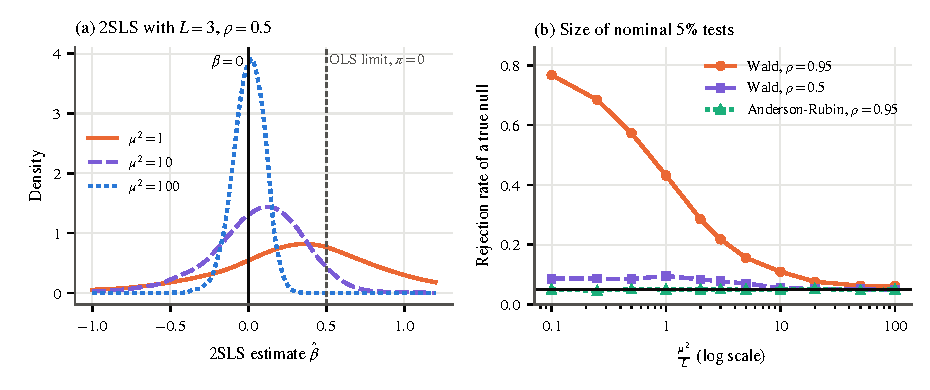
\includegraphics[width=\textwidth]{figures/appA/weakiv.pdf}
\caption{Weak instruments in a simulated design. The model is $y = x\beta + e$, $x = Z\pi + v$ with $\beta = 0$,
$n = 500$, three fixed standard normal instruments, and $(e_i, v_i)$ bivariate normal with unit variances and
correlation $\rho$. The vector $\pi$ is scaled to hit each concentration parameter $\mu^2$ exactly. (a) Kernel
densities of 2SLS over 10,000 replications for $\mu^2 \in \{1, 10, 100\}$ with $\rho = 0.5$. The dashed line marks
$\rho = 0.5$, the OLS limit with irrelevant instruments. (b) Rejection rates of nominal 5 percent tests of the
true null $\beta = 0$, plotted against $\frac{\mu^2}{L}$ on a log scale. The Wald test uses homoskedastic 2SLS
standard errors with $\rho = 0.95$ and $\rho = 0.5$, and the Anderson-Rubin test uses $\rho = 0.95$. The horizontal line is
the nominal size. The Monte Carlo standard error of a rejection rate of 0.05 is 0.0022. Seed 20261022, script
\texttt{sim\_iv.py}.}
\label{fig:A-weakiv}
\end{figure}

\casehead{Diagnostics}
The standard diagnostic is the first-stage $F$ statistic for the excluded instruments.
\citet{StaigerStock1997} suggest treating $F < 10$ as a sign of weak instruments, which by
\cref{prop:A-weak-bias} corresponds to a relative bias of roughly 10 percent. \citet{StockYogo2005} tabulate
cutoffs for the Cragg-Donald version of the statistic under homoskedasticity, for chosen tolerances on
the relative bias of 2SLS or on the size of Wald tests. With heteroskedastic, serially correlated or
clustered errors, the homoskedastic $F$ is invalid. Practitioners then report the robust Wald statistic of
\citet{KleibergenPaap2006}, divided by $L$, and compare it informally with the Stock-Yogo values.
\citet{MontielOleaPflueger2013} derive an \emph{effective} $F$ statistic with valid cutoffs for one
endogenous regressor. With several endogenous regressors, every first-stage $F$ can be large while the
instruments still fail to separate the regressors from one another. The conditional $F$ statistics of
\citet{SandersonWindmeijer2016} address this case. They are needed in the nested logit regression, where both
price and the log within-nest share are endogenous (\cref{sec:07-nl-estimation}). \Cref{tab:A-weakiv}
summarizes the rules.

\begin{table}[htbp]
\centering
\caption{Weak-instrument diagnostics and conventional thresholds}
\label{tab:A-weakiv}
\footnotesize
\begin{tabularx}{\textwidth}{@{}>{\raggedright\arraybackslash}p{0.2\textwidth}
>{\raggedright\arraybackslash}X >{\raggedright\arraybackslash}X >{\raggedright\arraybackslash}p{0.17\textwidth}@{}}
\toprule
Diagnostic & Setting & Threshold & Source \\
\midrule
First-stage $F$ on excluded instruments & One endogenous regressor, homoskedastic errors & $F > 10$ as a rule of
thumb & \citet{StaigerStock1997} \\
\addlinespace
Cragg-Donald $F$ with tabulated cutoffs & Homoskedastic errors, one or more endogenous regressors &
With one endogenous regressor, 9.08 for relative bias of at most 10 percent when $L = 3$, and 16.38
($L = 1$) or 22.30 ($L = 3$) for a nominal 5 percent Wald test with true size of at most 10 percent &
\citet[Tables~5.1--5.2]{StockYogo2005} \\
\addlinespace
Kleibergen-Paap Wald $F$ & Heteroskedastic or clustered errors & No formal cutoffs, compared informally with
the Stock-Yogo values & \citet{KleibergenPaap2006} \\
\addlinespace
Effective $F$ & One endogenous regressor with heteroskedastic, serially correlated or clustered errors & 23.1
as a conservative rule for a 2SLS Nagar bias of at most 10 percent of a worst-case benchmark, at the 5 percent
level & \citet[p.~358]{MontielOleaPflueger2013} \\
\addlinespace
Conditional $F$ & Several endogenous regressors & With $K = 2$, each statistic compared with the Stock-Yogo values
for one endogenous regressor and $L - 1$ instruments & \citet[Section~4]{SandersonWindmeijer2016} \\
\addlinespace
$tF$ adjustment & Just identified, one endogenous regressor & $F > 104.7$ for the usual cutoff of 1.96 to give a
true 5 percent test & \citet{LeeEtAl2022} \\
\bottomrule
\end{tabularx}

\smallskip
\begin{minipage}{0.92\textwidth}\footnotesize
Notes: $L$ is the number of excluded instruments and $K$ the number of endogenous regressors. The cutoffs
depend on the number of instruments and on the chosen tolerance, and the cited sources give full tables.
\end{minipage}
\end{table}

The first-stage $R^2$ is not a weak-instrument diagnostic, because it includes the explanatory power of the
exogenous regressors. \citet[WP fn.~23]{ChaudhuriGoldbergJia2006} report first-stage $R^2$ between 0.57 and 0.95
for their product-group prices, and 0.17 for domestic ciprofloxacin. Their instrument list includes
region-by-product dummies (WP p.~20), which can explain much of the variation in price levels on their own. What
matters is the contribution of the excluded instruments, measured by the partial $R^2$ or the partial $F$
statistic after the exogenous regressors are partialled out. An overall $F$ can also hide weak subsets. In
the simulated markets of \cref{app:problems}, the cluster-robust first-stage $F$ for seven excluded instruments
is 92.5, but six of them are jointly weak with $F = 2.32$. Nearly all the strength comes from one cost shifter.

\casehead{Inference that is robust to weak instruments}
The \emph{Anderson-Rubin test} \citep{AndersonRubin1949} remains valid however weak the instruments are. To test
$H_0\colon\beta = \beta_0$, form $\tilde y = y - x\beta_0$, which equals $e$ under the null. Regress $\tilde y$ on $Z$
and test that all coefficients are zero:
\begin{equation}\label{eq:A-ar}
AR(\beta_0) = \frac{\frac{1}{L}\tilde y^\top P_Z\tilde y}{\frac{1}{n - L}\tilde y^\top M_Z\tilde y} .
\end{equation}
Suppose the errors are normal, homoskedastic and independent of $Z$. Under $H_0$,
$\frac{1}{\sigma_e^2}e^\top P_Ze \sim \chi^2_L$ and $\frac{1}{\sigma_e^2}e^\top M_Ze \sim \chi^2_{n - L}$, because $P_Z$ and
$M_Z$ are idempotent with ranks $L$ and $n - L$. The two quadratic forms are independent because $P_ZM_Z = 0$.
Hence $AR(\beta_0) \sim F(L, n - L)$ exactly, whatever the value of $\pi$. With $K_1$ exogenous regressors partialled
out, the denominator degrees of freedom become $n - L - K_1$. Without normality, $L \cdot AR(\beta_0)$ is
asymptotically $\chi^2_L$, and heteroskedasticity- or cluster-robust versions use a robust Wald test of the
coefficients on $Z$.

A confidence set collects the values $\beta_0$ that the test does not reject. The Anderson-Rubin set can be a
bounded interval, the union of two rays, the whole real line, or even empty. An unbounded set is the right
answer when the data carry little information about $\beta$. In panel (b) of \cref{fig:A-weakiv}, the
Anderson-Rubin test rejects between 4.7 and 5.3 percent of the time at every instrument strength. Its
weakness is power when $L > K$, because it tests $\beta = \beta_0$ jointly with the overidentifying restrictions.
The conditional likelihood ratio test of \citet{Moreira2003} is more powerful, and it coincides with the
Anderson-Rubin test in the just-identified case. \citet{AndrewsStockSun2019} survey these methods.

\casehead{Many instruments}
Adding instruments that carry little information raises $L$ without raising $\mu^2$, and by
\cref{prop:A-weak-bias} it pushes 2SLS toward OLS. In the limit with as many instruments as observations,
$P_Z = I_n$ and 2SLS equals OLS. Limited-information maximum likelihood (LIML) is approximately median-unbiased
and much less sensitive to the number of instruments. The jackknife IV estimator removes the own-observation
term that causes the bias \citep{AngristImbensKrueger1999}. In demand estimation, \citet{Armstrong2016} shows
that the characteristics of rival products can be weak instruments in markets with many products. Markups then
converge to limits that hardly depend on rivals' characteristics (\cref{sec:08-iv-families}).

\subsection{Specification tests}\label{sec:A-spectests}

\casehead{Overidentification}
When $L > K$, the instruments imply more moment conditions than parameters, and we can test whether they are
mutually consistent. Under homoskedasticity, the \emph{Sargan statistic} is $n$ times the $R^2$ of the
regression of the 2SLS residuals on all instruments. It converges to $\chi^2_{L - K}$ under the null that every
instrument is exogenous \citep{Sargan1958}. Hansen's $J$ statistic is the robust version
(\cref{thm:A-jtest}). \citet[pp.~23--24]{Dafny2005} splits her instrument into the number of rival pairs less than
0.2 miles apart and the number between 0.2 and 0.3 miles apart. The Sargan statistic is 0.36 with a $p$-value
of 0.55, so the two bands imply similar effects. The test has limits. It is identically zero in a
just-identified model. It has no power against a bias that all instruments share. Both of Dafny's bands
measure distances between the same hospitals, so they would fail together if co-location itself were
correlated with unobserved price growth.

\casehead{The Hausman principle}
A second family of tests compares two estimators. One is efficient under the null hypothesis, and the other
is consistent under both the null and the alternative.

\begin{lemma}[Hausman]\label{lem:A-hausman}
Let $\hat\beta_E$ and $\hat\beta_C$ be estimators of $\beta$ such that, under $H_0$,
$\sqrt{n}\bigl((\hat\beta_E - \beta)^\top, (\hat\beta_C - \beta)^\top\bigr)^\top$ converges to a normal vector with
variances $V_E$ and $V_C$ and cross-covariance $C = \mathrm{Acov}(\hat\beta_E, \hat\beta_C)$. Here $\mathrm{Avar}$
and $\mathrm{Acov}$ denote the asymptotic variance and covariance of $\sqrt{n}$ times the centered estimators. If $\hat\beta_E$ is
asymptotically efficient under $H_0$, then $C = V_E$. Equivalently, $\hat\beta_E$ is asymptotically uncorrelated
with $\hat\beta_C - \hat\beta_E$, and
\begin{equation}\label{eq:A-hausman-var}
\mathrm{Avar}(\hat\beta_C - \hat\beta_E) = V_C - V_E .
\end{equation}
\end{lemma}

\begin{proof}
Write $D = \hat\beta_C - \hat\beta_E$, which converges to zero under $H_0$. Its asymptotic covariance with
$\hat\beta_E$ is $C - V_E$. For fixed vectors $a$ and $b$ and a scalar $\lambda$, the estimator
$a^\top\hat\beta_E + \lambda b^\top D$ is consistent for $a^\top\beta$. Its asymptotic variance is
\begin{equation*}
f(\lambda) = a^\top V_Ea + 2\lambda\,a^\top(C - V_E)b + \lambda^2\,b^\top\mathrm{Avar}(D)\,b .
\end{equation*}
Efficiency of $\hat\beta_E$ requires $f(\lambda) \ge f(0)$ for every $\lambda$, so the derivative at zero,
$2a^\top(C - V_E)b$, must vanish. This holds for all $a$ and $b$, so $C = V_E$. Then
$\mathrm{Avar}(D) = V_C - C - C^\top + V_E = V_C - V_E$.
\end{proof}

The \emph{Hausman statistic} is
\begin{equation}\label{eq:A-hausman}
\mathcal{H} = (\hat\beta_C - \hat\beta_E)^\top\bigl[\hat V_C - \hat V_E\bigr]^{-}(\hat\beta_C - \hat\beta_E)
\xrightarrow{d} \chi^2_q ,
\end{equation}
where $\hat V_C$ and $\hat V_E$ estimate the finite-sample variances, the superscript denotes a generalized
inverse, and $q$ is the rank of $V_C - V_E$ \citep{Hausman1978}. When OLS is compared with 2SLS, $q$ equals the
number of endogenous regressors tested. Two practical problems arise. The estimated difference
$\hat V_C - \hat V_E$ need not be positive semidefinite in finite samples, and OLS is efficient only under
homoskedasticity. The regression form avoids both. Add the first-stage residuals of the suspect regressors to
the OLS regression, as in \cref{prop:A-cf-2sls}, and test that their coefficients are jointly zero with a
robust Wald test. Under homoskedasticity this test is asymptotically equivalent to \eqref{eq:A-hausman}.

The principle appears throughout the book.
\begin{itemize}
\item \citet{Borenstein1989} rejects exogeneity of the route share and the route Herfindahl index, and so
  reports 2SLS. A Hausman test does not reject exogeneity of the load factor ``at any reasonable significance
  level'', so he treats it as exogenous (pp.~352 and 356--357). The cost of instrumenting shows in his Table 2.
  For the 80th percentile fare, the route-share coefficient is 0.1259 (0.0349) by OLS and 0.2238 (0.0784) by
  2SLS. The route Herfindahl coefficient moves from $-0.0120$ (0.0425) to $-0.1787$ (0.0901). The 2SLS standard
  errors are more than twice the OLS ones.
\item \citet[p.~21]{Dafny2005} reports that Hausman tests easily reject equality of the IV and OLS estimates
  in \cref{tab:A-dafny}.
\item \citet{Hausman1997} notes that weekly supermarket prices may be predetermined with respect to demand
  shocks, in which case OLS is consistent and efficient. A Hausman test of OLS against IV can decide
  (\cref{sec:10-hausman-identification}).
\item In panel data, random effects is efficient under its assumptions and fixed effects is consistent
  whether or not the unit effects are correlated with the regressors. Their difference tests
  $\E[\alpha_i \mid x_{i1}, \dots, x_{iT}] = 0$ (\cref{sec:A-panel}).
\item The test of independence of irrelevant alternatives of \citet{HausmanMcFadden1984} compares logit
  estimates from the full choice set with estimates from a restricted set. The restricted estimates are
  consistent under both hypotheses and inefficient under the null (\cref{eq:10-hm-test}).
\end{itemize}

\subsection{What IV estimates when effects differ}\label{sec:A-late}

So far the effect of $x_i$ has been the same for every unit. When effects differ, IV estimates a weighted
average of them, and the weights depend on the instrument.

\begin{theorem}[Local average treatment effect]\label{thm:A-late}
Let $z_i$ and $d_i$ be binary. Each unit has potential treatments $d_i(1)$ and $d_i(0)$, one for each value of
the instrument, and potential outcomes $y_i(d, z)$. Assume the following.
\begin{enumerate}[label=(\roman*)]
\item The instrument is independent of the potential outcomes and treatments
  $\{y_i(d, z), d_i(z) : d, z \in \{0, 1\}\}$.
\item The instrument is excluded from the outcome, $y_i(d, 1) = y_i(d, 0) \equiv y_i(d)$ for $d = 0, 1$.
\item The instrument is relevant, $\E[d_i(1) - d_i(0)] \neq 0$.
\item Treatment is monotone in the instrument, $d_i(1) \ge d_i(0)$ for every $i$.
\end{enumerate}
Then the Wald estimand \eqref{eq:A-wald-estimator} equals
$\E[y_i(1) - y_i(0) \mid d_i(1) > d_i(0)]$, the average effect for \emph{compliers}, the units whose treatment
the instrument changes \citep{ImbensAngrist1994}.
\end{theorem}

\begin{proof}
By exclusion, the observed outcome is $y_i = y_i(0) + d_i(z_i)\bigl(y_i(1) - y_i(0)\bigr)$. By independence,
\begin{equation*}
\E[y_i \mid z_i = 1] - \E[y_i \mid z_i = 0] = \E\bigl[\bigl(d_i(1) - d_i(0)\bigr)\bigl(y_i(1) - y_i(0)\bigr)\bigr] .
\end{equation*}
Monotonicity makes $d_i(1) - d_i(0)$ equal to one for compliers and zero for everyone else, so the right side
equals $\Pr(\text{complier})\,\E[y_i(1) - y_i(0) \mid \text{complier}]$. Independence also gives
$\E[d_i \mid z_i = 1] - \E[d_i \mid z_i = 0] = \E[d_i(1) - d_i(0)] = \Pr(\text{complier})$, which is nonzero by
relevance. The ratio is the complier average effect.
\end{proof}

The population splits into \emph{always-takers} ($d_i(1) = d_i(0) = 1$), \emph{never-takers}
($d_i(1) = d_i(0) = 0$), compliers, and \emph{defiers} ($d_i(1) < d_i(0)$), whom monotonicity rules out.
Different instruments move different compliers, so two valid instruments can identify different averages, and
an overidentification test can then reject even though both instruments are exogenous. With a continuous
endogenous variable, \citet{AngristGraddyImbens2000} show that the linear IV estimand in a supply and demand
system is a weighted average of the derivatives of the structural function. The weights are largest at
prices where the instrument shifts the equilibrium most. Dafny's estimate is local in this sense, since the
instrument moves only mergers of co-located hospitals.

\casehead{An IO analogue}
\citet{Corts1999} makes the same point about conduct. Write the supply relation as $P_t - c_t = \theta_tm_t$, with
conduct $\theta_t$ and $m_t = Q_t\bigl\lvert\frac{\partial Q_t}{\partial P_t}\bigr\rvert^{-1}$. Suppose marginal cost is known and a
demand shifter $Z_t$ serves as the instrument for $m_t$ in an equation with a constant conduct parameter. The
IV estimand is
\begin{equation*}
\frac{\Cov(Z_t, P_t - c_t)}{\Cov(Z_t, m_t)} = \frac{\Cov(Z_t, \theta_tm_t)}{\Cov(Z_t, m_t)} ,
\end{equation*}
which for small demand movements is approximately $\frac{\dd(\theta m)}{\dd m} = \theta + m\frac{\dd\theta}{\dd m}$.
The estimator recovers the marginal response of the markup to demand, which can differ sharply from the average
level of conduct. If $\theta_t = a - b\,m_t$, then $\theta_tm_t = am_t - bm_t^2$ and the estimand is
$a - b\frac{\Cov(Z_t, m_t^2)}{\Cov(Z_t, m_t)}$. With $\bar m = \E[m_t]$,
\begin{equation*}
\Cov(Z_t, m_t^2) = 2\bar m\Cov(Z_t, m_t) + \E\bigl[(Z_t - \E Z_t)(m_t - \bar m)^2\bigr] .
\end{equation*}
When the last term is zero, for example when $(Z_t, m_t)$ is jointly symmetric about its mean, the estimand is
$a - 2b\bar m$, while average conduct is $a - b\bar m$ (\cref{sec:03-corts}). Otherwise the third-moment term moves the
estimand away from $a - 2b\bar m$. In both cases the estimand can lie outside the range of $\theta_t$.

\subsection{System IV: three-stage least squares}\label{sec:A-3sls}

When several equations each contain endogenous regressors, they can be estimated jointly. Stack $G$ equations
$y_g = X_g\beta_g + e_g$ with a common $n \times L$ instrument matrix $Z$, block-diagonal $X$, and error vector
$e_t = (e_{1t}, \dots, e_{Gt})^\top$ with $\E[e_te_t^\top \mid z_t] = \Sigma$. The moment conditions are
$\E[e_t \otimes z_t] = 0$, and under conditional homoskedasticity their covariance matrix is
$\E[(e_t \otimes z_t)(e_t \otimes z_t)^\top] = \Sigma \otimes \E[z_tz_t^\top]$. Efficient GMM (\cref{sec:A-gmm-efficient}) weights the
sample moments $(I_G \otimes Z^\top)(y - X\beta)$ by the inverse of this matrix, estimated by
$\hat\Sigma^{-1} \otimes (Z^\top Z)^{-1}$. Since
$(I_G \otimes Z)(\hat\Sigma^{-1} \otimes (Z^\top Z)^{-1})(I_G \otimes Z^\top) = \hat\Sigma^{-1} \otimes P_Z$, the first-order
condition gives the \emph{three-stage least squares} (3SLS) estimator of \citet{ZellnerTheil1962},
\begin{equation}\label{eq:A-3sls}
\hat\beta_{3SLS} = \bigl[X^\top(\hat\Sigma^{-1} \otimes P_Z)X\bigr]^{-1}X^\top(\hat\Sigma^{-1} \otimes P_Z)\,y .
\end{equation}
The three stages are the first-stage regressions, 2SLS for each equation to estimate
$\hat\Sigma_{gh} = \frac{1}{n}\hat e_g^\top\hat e_h$, and the system estimator \eqref{eq:A-3sls}. By the logic of
\cref{prop:A-sur-ols}, 3SLS equals equation-by-equation 2SLS when $\Sigma$ is diagonal or every equation is
exactly identified. Its gains come from correlated errors and from restrictions across equations. Its cost is
that misspecification of any one equation contaminates the estimates of all of them. The estimated $\Sigma$
also adds noise in small samples.

\casehead{Application: residual demand in brewing}
\citet{BakerBresnahan1988} estimate the inverse residual demand curves of Anheuser-Busch, Pabst and Coors
jointly by 3SLS. Each equation regresses the firm's log price on its log quantity, demand shifters and cost
variables. The coefficient on own quantity, $\eta^R_j$, is the inverse elasticity of residual demand. Own
quantity is instrumented by firm-specific cost shifters: capacity for every firm, average plant size for
Anheuser-Busch and Pabst, and the Colorado manufacturing wage for Coors, which brewed only in Golden. The joint
estimation exploits the correlation of errors across the three equations. It also imposes a cross-equation
restriction, under which industry cost variables enter every equation through one common marginal cost index
(their eq.~12). The data are annual for 1962--1982, so each equation has only 21 observations (Table 3).

The estimates of $\eta^R_j$ are $-0.745$ (0.054) for Coors, $-0.058$ (0.031) for Pabst and $-0.312$ (0.064) for
Anheuser-Busch before 1975. An interaction with the post-1975 period, when light beer was introduced, is 0.282
(0.040), so Anheuser-Busch's inverse elasticity falls to $-0.030$ after 1975 (Table 3). Single-equation 2SLS gives
similar elasticities ``with little noticeable efficiency loss'' (fn.~20). Treating quantity as exogenous gives
$-0.738$, $-0.053$ and $-0.312$ (fn.~26), so simultaneity bias is small in these data. With 21 observations per
equation, several regressors and an estimated three-by-three covariance matrix, the asymptotic standard errors
should be read with caution. \Cref{sec:03-residual-demand} interprets the results.

The estimators of this section all have closed forms. Many structural models in industrial organization do not.
Their parameters enter nonlinearly, their errors enter through an equilibrium, or their likelihood involves an
integral. \Cref{sec:A-extremum} therefore turns to estimators defined by optimizing a criterion, which include
2SLS and 3SLS as special cases, and \cref{sec:A-twostep} returns to the joint estimation of demand and supply.

\section{Extremum estimators}\label{sec:A-extremum}

Almost every estimator in this book maximizes or minimizes a criterion function. Least squares minimizes a sum of squared
residuals. Maximum likelihood maximizes a log-likelihood. The BLP estimator minimizes a quadratic form in sample moments.
Simulated versions replace an intractable integral inside the criterion by an average over random draws. It pays to
prove consistency and asymptotic normality once, for the whole class, and then to read off each special case. This
section does that, following \citet{NeweyMcFadden1994}. As in the rest of the appendix, $\theta$ is a generic parameter
vector, here of dimension $K$, and the data $w_1, \dots, w_n$ are independent and identically distributed unless stated
otherwise. The convergence notation is the one set out in the introduction to this appendix.

\begin{definition}[Extremum estimator]\label{def:A-extremum}
Let $\Theta \subset \R^K$ be a parameter space and $Q_n(\theta)$ a criterion function that depends on the data. An
\emph{extremum estimator} is any $\hat\theta \in \Theta$ with
\begin{equation}\label{eq:A-extremum}
  Q_n(\hat\theta) \ge \sup_{\theta \in \Theta} Q_n(\theta) - o_p(1).
\end{equation}
The \emph{limit criterion} is a nonrandom function $Q_0(\theta)$ to which $Q_n(\theta)$ converges in probability.
\end{definition}

The $o_p(1)$ slack in \eqref{eq:A-extremum} allows for numerical optimization that stops close to, but not exactly at, the
supremum. This slack is enough for consistency. Asymptotic normality needs a tighter optimization tolerance, condition (v)
of \cref{thm:A-asy-normal}. The leading examples are the following.
\begin{enumerate}
  \item \emph{Nonlinear least squares} sets $Q_n(\theta) = -\frac{1}{n}\sum_{i=1}^n\{y_i - m(x_i;\theta)\}^2$, with limit
  $Q_0(\theta) = -\E[\{y_i - m(x_i;\theta)\}^2]$. Ordinary least squares is the case $m(x;\theta) = x^\T\theta$.
  \item \emph{Maximum likelihood} sets $Q_n(\theta) = \frac{1}{n}\sum_{i=1}^n\ln f(y_i \mid x_i;\theta)$, with limit
  $Q_0(\theta) = \E[\ln f(y_i \mid x_i;\theta)]$ (\cref{sec:A-mle}).
  \item The \emph{generalized method of moments} sets
  $Q_n(\theta) = -\bar g_n(\theta)^\T W_n\bar g_n(\theta)$, with limit
  $Q_0(\theta) = -\E[g(w_i;\theta)]^\T W\E[g(w_i;\theta)]$ (\cref{sec:A-gmm}). Here
  $\bar g_n(\theta) = \frac{1}{n}\sum_i g(w_i;\theta)$, and $W_n$ is a weighting matrix.
  \item \emph{Simulated estimators} use the same criteria with an expectation inside $g$ or $f$ replaced by a
  simulation average (\cref{sec:A-simulation}).
\end{enumerate}
The first two are \emph{M-estimators}, because $Q_n$ is a sample average of a function of one observation. GMM is a
\emph{minimum distance} estimator, because $Q_n$ is a quadratic form in sample averages. The general theorems below cover
both.

\subsection{Consistency}\label{sec:A-ext-consistency}

Consistency rests on two ideas. The limit criterion must have a unique maximum at the true value. The sample criterion
must be close to the limit criterion everywhere on the parameter space, not only at each point separately.

\begin{theorem}[Consistency of extremum estimators]\label{thm:A-consistency}
Suppose that (i) $Q_0(\theta)$ is uniquely maximized at $\theta_0$ (identification), (ii) $\Theta$ is compact, (iii)
$Q_0(\theta)$ is continuous, and (iv) $\sup_{\theta \in \Theta}\lvert Q_n(\theta) - Q_0(\theta)\rvert \xrightarrow{p} 0$
(uniform convergence). Then any extremum estimator satisfies $\hat\theta \xrightarrow{p} \theta_0$.
\end{theorem}

\begin{proof}
Fix $\epsilon > 0$. Three events occur w.p.a.1. By \eqref{eq:A-extremum},
$Q_n(\hat\theta) > Q_n(\theta_0) - \frac{\epsilon}{3}$. By uniform convergence,
$Q_0(\hat\theta) > Q_n(\hat\theta) - \frac{\epsilon}{3}$, since $\hat\theta \in \Theta$. Again by uniform convergence,
$Q_n(\theta_0) > Q_0(\theta_0) - \frac{\epsilon}{3}$. Chaining the three inequalities gives, w.p.a.1,
\begin{equation}\label{eq:A-consistency-chain}
  Q_0(\hat\theta) > Q_n(\hat\theta) - \frac{\epsilon}{3} > Q_n(\theta_0) - \frac{2\epsilon}{3} > Q_0(\theta_0) - \epsilon.
\end{equation}
Now let $\mathcal{N}$ be any open set that contains $\theta_0$. The set $\Theta \cap \mathcal{N}^c$ is closed and bounded,
hence compact. Since $Q_0$ is continuous, it attains its supremum on this set at some $\theta^*$. Identification gives
$Q_0(\theta^*) < Q_0(\theta_0)$. Choose $\epsilon = Q_0(\theta_0) - Q_0(\theta^*) > 0$. Then
\eqref{eq:A-consistency-chain} says that, w.p.a.1,
\begin{equation*}
  Q_0(\hat\theta) > Q_0(\theta^*) = \sup_{\theta \in \Theta \cap \mathcal{N}^c}Q_0(\theta).
\end{equation*}
So $\hat\theta \notin \Theta \cap \mathcal{N}^c$, that is, $\hat\theta \in \mathcal{N}$, w.p.a.1. Because $\mathcal{N}$ was
arbitrary, $\hat\theta \xrightarrow{p} \theta_0$.
\end{proof}

\Cref{fig:A-extremum} draws the argument. Uniform convergence traps $Q_n$ in a band of half-width $\epsilon$ around
$Q_0$. The maximizer of $Q_n$ must then achieve a value of $Q_0$ within $2\epsilon$ of the maximum, and identification
confines such points to a neighborhood of $\theta_0$ that shrinks with $\epsilon$.

\begin{figure}[htbp]
\centering
\begin{tikzpicture}
\begin{axis}[
  width=0.82\textwidth, height=6.2cm,
  xmin=0.2, xmax=3.8, ymin=0, ymax=2.75,
  axis lines=left, xlabel={$\theta$}, ylabel={criterion},
  xtick={0.8168, 2, 2.3087, 3.1832},
  xticklabels={$\theta_0 - r_\epsilon$, $\theta_0$, $\hat\theta$, $\theta_0 + r_\epsilon$},
  ytick={1.3, 2}, yticklabels={$Q_0(\theta_0) - 2\epsilon$, $Q_0(\theta_0)$},
  every tick label/.append style={font=\footnotesize},
  samples=200, domain=0.3:3.7, clip=false]
  \addplot[name path=up, draw=none, forget plot] {2 - 0.5*(x-2)^2 + 0.35};
  \addplot[name path=dn, draw=none, forget plot] {2 - 0.5*(x-2)^2 - 0.35};
  \addplot[blue!12, forget plot] fill between[of=up and dn];
  \addplot[blue!60!black, dashed, thin, forget plot] {2 - 0.5*(x-2)^2 + 0.35};
  \addplot[blue!60!black, dashed, thin, forget plot] {2 - 0.5*(x-2)^2 - 0.35};
  \addplot[black, very thick] {2 - 0.5*(x-2)^2};
  \addplot[orange!85!black, thick] {2 - 0.5*(x-2)^2 + 0.22*sin(deg(2.6*x+0.5)) + 0.1*sin(deg(6.3*x))};
  \draw[gray, densely dotted] (axis cs:0.2,1.3) -- (axis cs:3.8,1.3);
  \draw[gray, densely dotted] (axis cs:0.2,2) -- (axis cs:2,2);
  \draw[gray, densely dotted] (axis cs:0.8168,0) -- (axis cs:0.8168,1.3);
  \draw[gray, densely dotted] (axis cs:3.1832,0) -- (axis cs:3.1832,1.3);
  \draw[gray, densely dotted] (axis cs:2,0) -- (axis cs:2,2);
  \draw[orange!85!black, densely dotted] (axis cs:2.3087,0) -- (axis cs:2.3087,2.092);
  \fill[orange!85!black] (axis cs:2.3087,2.092) circle (1.6pt);
  \draw[very thick, gray!70] (axis cs:0.8168,0.06) -- (axis cs:3.1832,0.06);
  \draw[black, thin] (axis cs:3.0,1.5) -- (axis cs:3.45,2.05);
  \node[font=\footnotesize, anchor=south west] at (axis cs:3.42,2.03) {$Q_0(\theta)$};
  \draw[orange!85!black, thin] (axis cs:0.9,1.402) -- (axis cs:0.6,1.95);
  \node[font=\footnotesize, anchor=south, text=orange!85!black] at (axis cs:0.6,1.93) {$Q_n(\theta)$};
  \node[font=\footnotesize, anchor=south, text=blue!60!black] at (axis cs:2.2,2.4) {$Q_0(\theta) \pm \epsilon$};
\end{axis}
\end{tikzpicture}
\caption[The consistency argument for extremum estimators]{The consistency argument for extremum estimators. The thick
curve is the limit criterion $Q_0$, maximized only at $\theta_0$. Uniform convergence places the sample criterion $Q_n$
inside the shaded band $Q_0 \pm \epsilon$. The maximizer $\hat\theta$ of $Q_n$ then satisfies $Q_0(\hat\theta) > Q_0(\theta_0)
- 2\epsilon$, so it lies in the interval $[\theta_0 - r_\epsilon, \theta_0 + r_\epsilon]$ marked on the horizontal axis.
The curves are illustrative: $Q_0(\theta) = 2 - \frac{1}{2}(\theta - 2)^2$ and $\epsilon = 0.35$.}
\label{fig:A-extremum}
\end{figure}

Pointwise convergence of $Q_n(\theta)$ to $Q_0(\theta)$ at each $\theta$ is not enough. Take $\Theta = [0, 2]$ and
\begin{equation*}
  Q_n(\theta) = -\theta^2 + 2\max\left\{0,\ 1 - n\left\lvert\theta - 1 - \frac{1}{n}\right\rvert\right\}.
\end{equation*}
At each fixed $\theta$ the spike eventually moves away, so $Q_n(\theta) \to Q_0(\theta) = -\theta^2$, which is maximized at
$0$. Yet $Q_n(1 + \frac{1}{n}) = 2 - (1 + \frac{1}{n})^2$ is close to $1$, above $Q_n(0) = 0$. The maximizer converges to
$1$, not to $0$. Uniform convergence fails because $\sup_\theta\lvert Q_n - Q_0\rvert = 2$ for every $n$.

Uniform convergence is usually verified with a uniform law of large numbers. The next lemma is the version we use most
often. It is \citet[Lemma 2.4]{NeweyMcFadden1994}.

\begin{lemma}[Uniform law of large numbers]\label{lem:A-ulln}
Let $w_i$ be i.i.d., $\Theta$ compact, and $a(w, \theta)$ continuous in $\theta$ at each $\theta \in \Theta$ with
probability one. If $\E[\sup_{\theta \in \Theta}\lVert a(w_i, \theta)\rVert] < \infty$, then $\E[a(w_i, \theta)]$ is
continuous and
\begin{equation*}
  \sup_{\theta \in \Theta}\left\lVert\frac{1}{n}\sum_{i=1}^n a(w_i, \theta) - \E[a(w_i, \theta)]\right\rVert
  \xrightarrow{p} 0.
\end{equation*}
\end{lemma}

The integrable envelope $\sup_\theta\lVert a(w, \theta)\rVert$ is the \emph{dominance condition}. Continuity and compactness
let us cover $\Theta$ by finitely many small balls. On each ball the function moves little, and the ordinary law of large
numbers applies at the finitely many centers. For maximum likelihood we apply the lemma to $a = \ln f$. For GMM we apply
it to $a = g$ and then use the continuity of the quadratic form.

Compactness is a nuisance in practice, since few applied parameter spaces are bounded. For concave criteria it can be
dropped. This matters for the logit and multinomial logit likelihoods, which are globally concave
(\cref{prop:A-logit-concave}).

\begin{theorem}[Consistency with a concave criterion]\label{thm:A-concave}
Suppose that $\theta_0$ is an interior point of a convex set $\Theta$, $Q_n(\theta)$ is concave on $\Theta$ for each $n$,
$Q_n(\theta) \xrightarrow{p} Q_0(\theta)$ for each $\theta \in \Theta$, and $Q_0$ is uniquely maximized at $\theta_0$. Then
$\hat\theta$ exists w.p.a.1 and $\hat\theta \xrightarrow{p} \theta_0$.
\end{theorem}

The proof \citep[Theorem 2.7]{NeweyMcFadden1994} uses a fact from convex analysis. Pointwise convergence of concave
functions implies uniform convergence on compact subsets of the interior. Apply \cref{thm:A-consistency} on a small closed
ball around $\theta_0$. Concavity then rules out a maximizer outside the ball. A concave function that is higher at the
center of a ball than everywhere on its boundary is also higher at the center than anywhere outside the ball.

Identification, condition (i), is the substantive assumption. It says that the model and the data distribution single
out $\theta_0$. \Cref{sec:A-identification} discusses what it requires in IO models. Conditions (ii) to (iv) are
regularity conditions that hold in most smooth applications.

\subsection{Asymptotic normality}\label{sec:A-ext-normality}

Once $\hat\theta$ is consistent, a Taylor expansion of the first-order condition around $\theta_0$ delivers its limit
distribution.

\begin{theorem}[Asymptotic normality of extremum estimators]\label{thm:A-asy-normal}
Suppose the following conditions hold.
\begin{enumerate}[label=(\roman*)]
  \item $\hat\theta \xrightarrow{p} \theta_0$, and $\theta_0$ is in the interior of $\Theta$.
  \item $Q_n(\theta)$ is twice continuously differentiable on a neighborhood $\mathcal{N}$ of $\theta_0$.
  \item $\sqrt{n}\,\nabla_\theta Q_n(\theta_0) \xrightarrow{d} N(0, \Sigma)$.
  \item There is a matrix function $H(\theta)$, continuous at $\theta_0$, with $\sup_{\theta \in
  \mathcal{N}}\lVert\nabla_{\theta\theta}Q_n(\theta) - H(\theta)\rVert \xrightarrow{p} 0$ and $H = H(\theta_0)$ nonsingular.
  \item $\sqrt{n}\,\nabla_\theta Q_n(\hat\theta) \xrightarrow{p} 0$. An exact interior maximizer satisfies this with
  $\nabla_\theta Q_n(\hat\theta) = 0$.
\end{enumerate}
Then
\begin{equation}\label{eq:A-sandwich}
  \sqrt{n}(\hat\theta - \theta_0) \xrightarrow{d} N\big(0,\ H^{-1}\Sigma H^{-1}\big).
\end{equation}
\end{theorem}

\begin{proof}
Because $\hat\theta \xrightarrow{p} \theta_0$ and $\theta_0$ is interior, $\hat\theta$ lies in $\mathcal{N}$ and in the
interior of $\Theta$ w.p.a.1. Write $r_n = \nabla_\theta Q_n(\hat\theta)$ for the gradient at the estimate. By (v),
$\sqrt{n}\,r_n \xrightarrow{p} 0$. Apply the mean value theorem to each element of the gradient. For row $k$ there is a point
$\bar\theta^{(k)}$ on the segment between $\hat\theta$ and $\theta_0$ with
\begin{equation*}
  r_{n,k} = \frac{\partial Q_n(\theta_0)}{\partial\theta_k} + \frac{\partial^2 Q_n(\bar\theta^{(k)})}{\partial\theta_k\partial\theta^\T}
  (\hat\theta - \theta_0).
\end{equation*}
Stack the rows into the matrix $\bar H_n$, whose row $k$ is the $k$-th row of the Hessian evaluated at $\bar\theta^{(k)}$.
Then
\begin{equation*}
  r_n = \nabla_\theta Q_n(\theta_0) + \bar H_n(\hat\theta - \theta_0).
\end{equation*}
Each $\bar\theta^{(k)}$ converges in probability to $\theta_0$. By (iv) and the continuity of $H$ at $\theta_0$,
\begin{equation*}
  \lVert\bar H_n - H\rVert \le \sup_{\theta \in \mathcal{N}}\lVert\nabla_{\theta\theta}Q_n(\theta) - H(\theta)\rVert
  + \max_k\lVert H(\bar\theta^{(k)}) - H\rVert \xrightarrow{p} 0.
\end{equation*}
So $\bar H_n$ is invertible w.p.a.1, and
\begin{equation*}
  \sqrt{n}(\hat\theta - \theta_0) = -\bar H_n^{-1}\sqrt{n}\,\nabla_\theta Q_n(\theta_0) + \bar H_n^{-1}\sqrt{n}\,r_n.
\end{equation*}
The second term converges in probability to zero by (v). By (iii), Slutsky's theorem and the continuous mapping theorem, the
right side converges in distribution to $-H^{-1}Z$ with $Z \sim N(0, \Sigma)$. Its variance is $H^{-1}\Sigma H^{-1}$, because
$H$ is symmetric.
\end{proof}

Condition (v) cannot be dropped. Take $Y_i$ i.i.d.\ $N(0,1)$, $\theta_0 = 0$, $Q_n(\theta) = -\frac{1}{2}(\theta - \bar Y)^2$,
and an optimizer that stops at $\hat\theta = \bar Y + n^{-\frac{1}{4}}$. The criterion shortfall is
$\frac{1}{2}n^{-\frac{1}{2}} = o(1)$, so $\hat\theta$ is a consistent extremum estimator and (i)--(iv) hold. Yet
$\sqrt{n}\,\hat\theta = \sqrt{n}\,\bar Y + n^{\frac{1}{4}}$ diverges. An optimization error that vanishes more slowly than
the sampling error swamps it. Under local quadratic curvature, a criterion shortfall of order $o_p(n^{-1})$ is enough for (v).

The variance in \eqref{eq:A-sandwich} is a \emph{sandwich}. The outer pieces measure the curvature of the criterion, the
inner piece the noise in its slope at the truth. A consistent estimator replaces $H$ by $\nabla_{\theta\theta}Q_n(\hat\theta)$
and $\Sigma$ by an estimate of the variance of $\sqrt{n}\,\nabla_\theta Q_n(\theta_0)$. For an M-estimator with
$Q_n = \frac{1}{n}\sum_i q(w_i;\theta)$, that estimate is $\frac{1}{n}\sum_i\nabla_\theta q(w_i;\hat\theta)
\nabla_\theta q(w_i;\hat\theta)^\T$. With dependent data it becomes a clustered or HAC estimate (\cref{sec:A-cluster,sec:A-hac}).

The theorem fails in three situations that occur in IO. If $\theta_0$ lies on the boundary of $\Theta$, the first-order
condition need not hold. A variance component or a regime probability equal to zero is the usual case
(\cref{sec:A-mle-nonregular}). If $Q_n$ is not differentiable, the expansion must be replaced by an argument based on
stochastic equicontinuity. Simulated frequency estimators and some auction estimators are examples
\citep{PakesPollard1989}. If $H$ is singular, the rank condition for local identification fails. The parameter
$\theta_0$ may still be identified through higher-order terms, but the normal approximation breaks down and the rate of
convergence changes.

\subsection{Profile objectives}\label{sec:A-profile}

Many IO estimators split the parameters into a block that is easy to optimize given the rest and a block that is hard.
Optimizing out the easy block first leaves a \emph{profile} (or \emph{concentrated}) criterion in the hard block alone.

\begin{proposition}[Profile criteria]\label{prop:A-profile}
Partition $\theta = (\theta_1, \theta_2)$ with $\Theta = \Theta_1 \times \Theta_2$. Suppose that for each $\theta_2$ the
maximizer $\hat\theta_1(\theta_2) = \argmax_{\theta_1 \in \Theta_1}Q_n(\theta_1, \theta_2)$ exists and is unique. Define the
profile criterion $\tilde Q_n(\theta_2) = Q_n(\hat\theta_1(\theta_2), \theta_2)$.
\begin{enumerate}[label=(\alph*)]
  \item $(\hat\theta_1, \hat\theta_2)$ maximizes $Q_n$ jointly if and only if $\hat\theta_2$ maximizes $\tilde Q_n$ and
  $\hat\theta_1 = \hat\theta_1(\hat\theta_2)$.
  \item Suppose $Q_n$ is twice continuously differentiable and that, on a neighborhood of $\theta_2$, $\hat\theta_1(\cdot)$ is
  continuous with values in the interior of $\Theta_1$. If the Hessian block $H_{11} = \nabla_{\theta_1\theta_1}Q_n$ is
  nonsingular at $(\hat\theta_1(\theta_2), \theta_2)$, then
  \begin{equation}\label{eq:A-profile-derivs}
    \nabla_{\theta_2}\tilde Q_n(\theta_2) = \nabla_{\theta_2}Q_n\big(\hat\theta_1(\theta_2), \theta_2\big),
    \qquad
    \nabla_{\theta_2\theta_2}\tilde Q_n(\theta_2) = H_{22} - H_{21}H_{11}^{-1}H_{12},
  \end{equation}
  where the blocks of the Hessian of $Q_n$ are evaluated at $(\hat\theta_1(\theta_2), \theta_2)$.
\end{enumerate}
\end{proposition}

\begin{proof}
(a) For any $(\theta_1, \theta_2)$,
\begin{equation*}
  Q_n(\theta_1, \theta_2) \le Q_n(\hat\theta_1(\theta_2), \theta_2) = \tilde Q_n(\theta_2).
\end{equation*}
Hence $\sup_{\theta}Q_n(\theta) = \sup_{\theta_2}\tilde Q_n(\theta_2)$. If $\hat\theta_2$ maximizes $\tilde Q_n$, then
$(\hat\theta_1(\hat\theta_2), \hat\theta_2)$ attains this common supremum. Conversely, if $(\hat\theta_1, \hat\theta_2)$
maximizes $Q_n$, then $\tilde Q_n(\hat\theta_2) \ge Q_n(\hat\theta_1, \hat\theta_2) = \sup_{\theta_2}\tilde Q_n$, and
uniqueness of the inner maximizer gives $\hat\theta_1 = \hat\theta_1(\hat\theta_2)$.

(b) Because the inner maximizer is interior, the inner first-order condition
$\nabla_{\theta_1}Q_n(\hat\theta_1(\theta_2), \theta_2) = 0$ holds on the neighborhood. The implicit function theorem gives
a locally unique $C^1$ solution of this condition. By continuity $\hat\theta_1(\cdot)$ coincides with it, and
differentiating the condition gives
\begin{equation*}
  H_{11}\frac{\partial\hat\theta_1}{\partial\theta_2^\T} + H_{12} = 0
  \quad\Longrightarrow\quad
  \frac{\partial\hat\theta_1}{\partial\theta_2^\T} = -H_{11}^{-1}H_{12}.
\end{equation*}
By the chain rule,
\begin{equation*}
  \nabla_{\theta_2}\tilde Q_n = \left(\frac{\partial\hat\theta_1}{\partial\theta_2^\T}\right)^\T\nabla_{\theta_1}Q_n
  + \nabla_{\theta_2}Q_n = \nabla_{\theta_2}Q_n,
\end{equation*}
because the first term vanishes by the inner first-order condition. This is the envelope theorem. Differentiating once
more,
\begin{equation*}
  \nabla_{\theta_2\theta_2}\tilde Q_n = H_{21}\frac{\partial\hat\theta_1}{\partial\theta_2^\T} + H_{22}
  = H_{22} - H_{21}H_{11}^{-1}H_{12}. \qedhere
\end{equation*}
\end{proof}

Part (a) is what makes nested estimation legitimate. Part (b) says how to get standard errors. By the partitioned
inverse formula, $(H_{22} - H_{21}H_{11}^{-1}H_{12})^{-1}$ is the $(2,2)$ block of $H^{-1}$. For maximum likelihood, where
the asymptotic variance is $(-H)^{-1}$, the inverse Hessian of the profile log-likelihood therefore gives the correct
variance for $\hat\theta_2$. It already accounts for the estimation of $\theta_1$. For GMM the full sandwich is needed,
and \cref{sec:A-gmm-computation} gives the formula.

Three applications recur in this book. In the normal linear regression, the variance $\sigma^2$ can be profiled out. The
log-likelihood at $\hat\sigma^2(\beta) = \frac{1}{n}\sum_i(y_i - x_i^\T\beta)^2$ is $-\frac{n}{2}\ln\hat\sigma^2(\beta)$ plus a
constant. This is the form behind the Cox statistic of \cref{prop:06-bres-cox}. In the BLP estimator, the linear demand
parameters have a closed form given the nonlinear ones (\cref{prop:08-concentrate}). In supply-side estimation with many
fixed effects, the effects and the linear cost parameters can be concentrated out by least squares.
\citet[p.~1780]{MillerWeinberg2017} do this when they estimate the internalization and cost parameters of the beer
industry after the MillerCoors joint venture (\cref{ch:mergers}).

Profiling does not cure an \emph{incidental parameters} problem. Suppose $y_{it} = \mu_i + e_{it}$ with
$e_{it} \sim N(0, \sigma^2)$, $i = 1, \dots, N$ and $t = 1, \dots, T$, with $T$ fixed and $N \to \infty$. Profiling out each
$\mu_i$ gives $\hat\mu_i = \bar y_i$ and
\begin{equation*}
  \hat\sigma^2 = \frac{1}{NT}\sum_{i=1}^N\sum_{t=1}^T(y_{it} - \bar y_i)^2 \xrightarrow{p} \frac{T - 1}{T}\sigma^2.
\end{equation*}
The estimator is inconsistent \citep{NeymanScott1948}. The number of profiled parameters grows with the sample, so the
fixed-dimension assumptions of \cref{thm:A-consistency} fail. In linear models the bias has a known form, but in nonlinear
models with many fixed effects it contaminates every parameter.

\subsection{Numerical practice}\label{sec:A-numerical}

The theorems describe the global maximizer. A computer returns a point where an algorithm stopped. The gap between the
two is a frequent source of error in structural IO, and good practice narrows it.

Gradient methods iterate $\theta^{(m+1)} = \theta^{(m)} - \lambda_m A_m^{-1}\nabla_\theta Q_n(\theta^{(m)})$, where
$\lambda_m > 0$ is a step length and $A_m$ approximates the Hessian. Newton's method uses the Hessian itself and converges
quadratically near a maximum with a negative definite Hessian. Quasi-Newton methods such as BFGS build $A_m$ from
successive gradients. For maximum likelihood, the method of \citet{BerndtEtAl1974} (BHHH) replaces the Hessian by minus
the outer product of the scores. That matrix is negative semidefinite by construction. By the information equality of
\cref{sec:A-mle-score}, it is consistent for the Hessian at the truth. Derivative-free methods such as Nelder and Mead's simplex need only
function values. They are slow but robust to kinks.

We recommend the following checks.
\begin{enumerate}
  \item Scale the parameters so that a unit change in each moves the criterion by similar amounts. Poor scaling
  makes gradient methods take tiny steps along flat directions.
  \item Use analytic gradients when possible. Finite differences lose about half the digits of the criterion.
  \item Start the optimizer from many points. If different starts end at different values, report the best and
  investigate the others. \citet[p.~309]{Porter1983} reports that his switching model converged to the same estimates
  from several disparate starting points. \citet{KnittelMetaxoglou2014} show that BLP estimates can depend on the
  optimizer and the starting values (\cref{ch:blp}).
  \item At the reported optimum, check that the gradient is close to zero and that the Hessian is negative definite.
  A singular Hessian signals that the rank condition for local identification fails.
  \item Hold simulation draws fixed across evaluations. Redrawing them makes the criterion change between calls, and the
  optimizer never settles (\cref{sec:A-simulation}).
  \item When the criterion contains an inner fixed point, such as the BLP contraction, solve the inner problem to a
  tight tolerance. Inner-loop error makes the outer criterion noisy and can produce false convergence
  \citep{DubeFoxSu2012}.
\end{enumerate}

Some criteria are not smooth at all. In the vertical model the ordering of products by quality depends on the quality
coefficients. When two products swap places, the predicted prices and quantities jump, and so does the likelihood
(\cref{sec:06-bres-estimation}). Gradient methods then behave erratically, and derivative-free search or a grid over the
offending parameters is safer. Frequency simulators produce step functions for the same reason, which is why smooth
simulators are preferred (\cref{sec:A-simulation}).

\section{Generalized method of moments}\label{sec:A-gmm}

The generalized method of moments (GMM) of \citet{Hansen1982} is the workhorse estimator of structural IO. It needs only
a set of population moment conditions implied by the model, and no full likelihood. Demand estimation with instruments,
supply relations with unobserved cost shocks, and their joint estimation all fit this mold.

\subsection{Moment conditions}\label{sec:A-gmm-moments}

\begin{definition}[Moment conditions]\label{def:A-moments}
Let $g(w;\theta)$ be an $L \times 1$ vector of functions of the data $w$ and the $K \times 1$ parameter $\theta$, with
$L \ge K$. The model implies the \emph{moment conditions}
\begin{equation}\label{eq:A-moments}
  \E[g(w_i;\theta_0)] = 0.
\end{equation}
The parameter is \emph{globally identified} by \eqref{eq:A-moments} if $\E[g(w_i;\theta)] \ne 0$ for every
$\theta \ne \theta_0$ in $\Theta$. It is \emph{locally identified} if the $L \times K$ Jacobian
$G = \E\big[\frac{\partial g(w_i;\theta_0)}{\partial\theta^\T}\big]$ has rank $K$.
\end{definition}

The \emph{order condition} $L \ge K$ is necessary for the rank condition. When $g$ is linear in $\theta$ the rank condition
gives global identification. When $g$ is nonlinear it gives only local identification (\cref{prop:A-local-id}), and
global identification must be argued separately. The applications in this book use the following moment functions.
\begin{enumerate}
  \item \emph{Least squares} uses $g(w_i;\beta) = x_i(y_i - x_i^\T\beta)$, with $L = K$.
  \item \emph{Linear instrumental variables} use $g(w_i;\beta) = z_i(y_i - x_i^\T\beta)$, with $z_i$ an $L \times 1$
  vector of instruments (\cref{sec:A-iv}).
  \item \emph{Nonlinear instrumental variables}. In the sugar study of \citet{GenesoveMullin1998}, demand is
  $Q = \beta(\alpha - P)^\gamma$ and marginal cost is $c_0 + kP^{\mathit{raw}}$. The pricing rule with conduct parameter
  $\theta$ is $P = \frac{\alpha\theta + c_0\gamma}{\gamma + \theta} + \frac{\gamma}{\gamma + \theta}kP^{\mathit{raw}}$. With
  $(\alpha, \gamma)$ set at their demand estimates, the moment function for $\psi = (\theta, c_0, k)$ is
  \begin{equation}\label{eq:A-sugar-moment}
    g(w_t;\psi) = z_t\left\{(\gamma + \theta)P_t - \alpha\theta - c_0\gamma - \gamma kP^{\mathit{raw}}_t\right\}.
  \end{equation}
  Here $z_t$ contains the log of Cuban raw-sugar imports, a high-season dummy and a constant (Genesove and Mullin, WP
  eq.~13). The raw price is instrumented because shocks to the pricing rule move it. Here $\theta$ is the conduct
  parameter of \cref{sec:03-sugar-neio}. Letting conduct differ in price-war periods replaces $\theta$ by
  $\theta_0 + (\theta_1 - \theta_0)\mathit{WAR}_t$ and adds the war dummy to $z_t$, which keeps the system just
  identified (\cref{sec:03-sugar-wars}).
  \item \emph{Demand moments in differentiated products}. With the logit inversion, the structural error is
  $\xi_{jt}(\theta) = \ln s_{jt} - \ln s_{0t} - x_{jt}\beta + \alpha p_{jt}$ (\cref{ch:logit}). With random coefficients,
  $\xi_{jt}(\theta) = \delta_{jt}(s_t;\theta_2) - x_{jt}\beta + \alpha p_{jt}$, where $\delta_{jt}(s_t;\theta_2)$ inverts
  the share system (\cref{ch:blp}). Either way $g = z_{jt}\xi_{jt}(\theta)$.
  \item \emph{Supply moments}. Under Bertrand-Nash pricing, marginal cost is price minus the markup implied by demand,
  $mc_{jt}(\theta) = p_{jt} + [(\Omega_t \odot \Delta_t^\top)^{-1}s_t]_j$. In this item $\Omega_t$ is the ownership
  matrix of market $t$, and $\Delta_t$ has $(j,k)$ element $\frac{\partial s_{jt}}{\partial p_{kt}}$
  (\cref{ch:diffprod}). If
  $mc_{jt} = w_{jt}\gamma + \omega_{jt}$, the cost moment is $g = z^s_{jt}\{mc_{jt}(\theta) - w_{jt}\gamma\}$.
  \item \emph{Conditional moment restrictions}. Many models state $\E[\rho(w_i;\theta_0) \mid z_i] = 0$ for a residual vector
  $\rho$. Any matrix of functions $A(z_i)$ then gives unconditional moments $\E[A(z_i)\rho(w_i;\theta_0)] = 0$. Which
  functions to use is the optimal instruments problem of \cref{sec:A-optimal-iv}.
  \item \emph{Simulated moments}, where an expectation inside $g$ is replaced by a simulation average
  (\cref{sec:A-simulation}).
\end{enumerate}

\subsection{The estimator and its asymptotic distribution}\label{sec:A-gmm-asy}

\begin{definition}[GMM estimator]\label{def:A-gmm}
Let $\bar g_n(\theta) = \frac{1}{n}\sum_{i=1}^n g(w_i;\theta)$ and let $W_n$ be a symmetric positive semidefinite
$L \times L$ matrix with $W_n \xrightarrow{p} W$. The \emph{GMM estimator} is
\begin{equation}\label{eq:A-gmm}
  \hat\theta = \argmin_{\theta \in \Theta}\ \bar g_n(\theta)^\T W_n\,\bar g_n(\theta).
\end{equation}
\end{definition}

Consistency follows from \cref{thm:A-consistency} with $Q_n(\theta) = -\bar g_n(\theta)^\T W_n\bar g_n(\theta)$ and
$Q_0(\theta) = -\E[g(\theta)]^\T W\E[g(\theta)]$, writing $\E[g(\theta)]$ for $\E[g(w_i;\theta)]$. The limit is
maximized, with value zero, at every $\theta$ where $W\E[g(\theta)] = 0$. Identification therefore requires
$W\E[g(\theta)] \ne 0$ for $\theta \ne \theta_0$, which holds when $W$ is positive definite and the moments identify
$\theta_0$. Uniform convergence follows from \cref{lem:A-ulln} applied to $g$, if $g$ is continuous in $\theta$ and
$\E[\sup_\theta\lVert g(w_i;\theta)\rVert] < \infty$. Indeed, adding and subtracting terms,
\begin{equation*}
  \lvert Q_n(\theta) - Q_0(\theta)\rvert
  \le \lVert\bar g_n - \E g\rVert^2\lVert W_n\rVert + 2\lVert\E g\rVert\,\lVert W_n\rVert\,\lVert\bar g_n - \E g\rVert
  + \lVert\E g\rVert^2\lVert W_n - W\rVert,
\end{equation*}
and each term converges to zero uniformly on the compact $\Theta$.

\begin{theorem}[Asymptotic normality of GMM]\label{thm:A-gmm-normal}
Suppose the following conditions hold.
\begin{enumerate}[label=(\roman*)]
  \item $\hat\theta \xrightarrow{p} \theta_0$, with $\theta_0$ interior.
  \item $g(w;\theta)$ is continuously differentiable in $\theta$ on a neighborhood $\mathcal{N}$ of $\theta_0$.
  \item $\sqrt{n}\,\bar g_n(\theta_0) \xrightarrow{d} N(0, S)$.
  \item $G_n(\theta) = \frac{\partial\bar g_n(\theta)}{\partial\theta^\T}$ satisfies $\sup_{\theta \in \mathcal{N}}\lVert
  G_n(\theta) - G(\theta)\rVert \xrightarrow{p} 0$ for a function $G(\theta)$ continuous at $\theta_0$.
  \item $W_n \xrightarrow{p} W$, and $G^\T WG$ is nonsingular, where $G = G(\theta_0)$.
\end{enumerate}
Then
\begin{equation}\label{eq:A-gmm-var}
  \sqrt{n}(\hat\theta - \theta_0) \xrightarrow{d} N(0, V), \qquad
  V = (G^\T WG)^{-1}G^\T WSWG(G^\T WG)^{-1}.
\end{equation}
\end{theorem}

\begin{proof}
W.p.a.1 the estimator is interior and satisfies the first-order condition of \eqref{eq:A-gmm},
\begin{equation*}
  G_n(\hat\theta)^\T W_n\,\bar g_n(\hat\theta) = 0.
\end{equation*}
A mean value expansion of each element of $\bar g_n(\hat\theta)$ around $\theta_0$ gives
\begin{equation*}
  \bar g_n(\hat\theta) = \bar g_n(\theta_0) + \bar G_n(\hat\theta - \theta_0),
\end{equation*}
where row $\ell$ of $\bar G_n$ is row $\ell$ of $G_n$ evaluated at a point between $\hat\theta$ and $\theta_0$. Substitute
into the first-order condition:
\begin{equation*}
  G_n(\hat\theta)^\T W_n\bar g_n(\theta_0) + G_n(\hat\theta)^\T W_n\bar G_n(\hat\theta - \theta_0) = 0.
\end{equation*}
By (i), (iv) and (v), $G_n(\hat\theta)^\T W_n\bar G_n \xrightarrow{p} G^\T WG$, which is nonsingular. Solve and multiply by
$\sqrt{n}$:
\begin{equation*}
  \sqrt{n}(\hat\theta - \theta_0) = -\big[G_n(\hat\theta)^\T W_n\bar G_n\big]^{-1}G_n(\hat\theta)^\T W_n\sqrt{n}\,\bar
  g_n(\theta_0).
\end{equation*}
By (iii) and Slutsky's theorem the right side converges in distribution to $-(G^\T WG)^{-1}G^\T WZ$ with $Z \sim N(0, S)$,
whose variance is $V$.
\end{proof}

With i.i.d.\ data, $S = \E[g(w_i;\theta_0)g(w_i;\theta_0)^\T]$, estimated by $\hat S = \frac{1}{n}\sum_i g(w_i;\hat\theta)
g(w_i;\hat\theta)^\T$. The Jacobian is estimated by $\hat G = G_n(\hat\theta)$. The plug-in $\hat V$ replaces each
population matrix by its estimate.

\casehead{Linear instrumental variables}
Stack the data as $y$ ($n \times 1$), $X$ ($n \times K$) and $Z$ ($n \times L$). Then $\bar g_n(\beta) = \frac{1}{n}Z^\T(y -
X\beta)$, and the criterion is $\frac{1}{n^2}(y - X\beta)^\T ZW_nZ^\T(y - X\beta)$. The first-order condition is
\begin{equation*}
  -\frac{2}{n^2}X^\T ZW_nZ^\T(y - X\beta) = 0,
\end{equation*}
so
\begin{equation}\label{eq:A-linear-gmm}
  \hat\beta = \big(X^\T ZW_nZ^\T X\big)^{-1}X^\T ZW_nZ^\T y.
\end{equation}
With $W_n = (\frac{1}{n}Z^\T Z)^{-1}$ this is two-stage least squares, \eqref{eq:A-2sls}, the third route of
\cref{sec:A-2sls}. Here $G = -\E[z_ix_i^\T]$, so \eqref{eq:A-gmm-var} becomes the IV sandwich of
\cref{prop:A-2sls-asy}. When $L = K$, the algebra of \cref{sec:A-2sls} shows that \eqref{eq:A-linear-gmm} collapses to
$(Z^\T X)^{-1}Z^\T y$ whatever $W_n$ is. The general lesson is that a just-identified GMM estimator sets
$\bar g_n(\hat\theta) = 0$, so the weighting matrix plays no role.

\subsection{Efficient weighting}\label{sec:A-gmm-efficient}

The weighting matrix matters only when $L > K$. It decides how to trade off moments that cannot all be set to zero in the
sample. The best choice weights each moment by the inverse of its noise.

\begin{proposition}[Efficient weighting matrix]\label{prop:A-efficient-gmm}
Under the assumptions of \cref{thm:A-gmm-normal} with $S$ positive definite, the asymptotic variance $V(W)$ in
\eqref{eq:A-gmm-var} satisfies $V(W) - (G^\T S^{-1}G)^{-1} \succeq 0$ for every admissible $W$. The lower bound is attained
at $W = S^{-1}$, where $V = (G^\T S^{-1}G)^{-1}$.
\end{proposition}

\begin{proof}
Define the $K \times L$ matrix
\begin{equation*}
  A = (G^\T WG)^{-1}G^\T W - (G^\T S^{-1}G)^{-1}G^\T S^{-1}.
\end{equation*}
Since $S$ is positive definite, $ASA^\T \succeq 0$. Expand the product term by term:
\begin{align*}
  ASA^\T &= (G^\T WG)^{-1}G^\T WSWG(G^\T WG)^{-1}
  - (G^\T WG)^{-1}G^\T WG(G^\T S^{-1}G)^{-1} \\
  &\quad - (G^\T S^{-1}G)^{-1}G^\T WG(G^\T WG)^{-1}
  + (G^\T S^{-1}G)^{-1}G^\T S^{-1}G(G^\T S^{-1}G)^{-1}.
\end{align*}
The first term is $V(W)$. After cancellation, each of the last three matrix products equals $(G^\T S^{-1}G)^{-1}$, and
they enter with signs minus, minus and plus. So $ASA^\T = V(W) - (G^\T S^{-1}G)^{-1}$, which is positive semidefinite.
Setting $W = S^{-1}$ in \eqref{eq:A-gmm-var} gives
\begin{equation*}
  V(S^{-1}) = (G^\T S^{-1}G)^{-1}G^\T S^{-1}SS^{-1}G(G^\T S^{-1}G)^{-1} = (G^\T S^{-1}G)^{-1}. \qedhere
\end{equation*}
\end{proof}

The efficient weight depends on $S$, which depends on $\theta_0$. Three feasible versions are in use.
\begin{enumerate}
  \item \emph{Two-step GMM}. Estimate $\tilde\theta$ with a fixed weight, such as $(\frac{1}{n}Z^\T Z)^{-1}$. Form
  \begin{equation*}
    \hat S = \frac{1}{n}\sum_{i=1}^ng(w_i;\tilde\theta)g(w_i;\tilde\theta)^\T
  \end{equation*}
  and re-estimate with $W_n = \hat S^{-1}$.
  \item \emph{Iterated GMM}. Repeat the second step, updating $\hat S$ each time, until the estimates stop changing.
  \item \emph{Continuously updated GMM} (CUE) of \citet{HansenHeatonYaron1996}. Minimize
  $\bar g_n(\theta)^\T\hat S(\theta)^{-1}\bar g_n(\theta)$, where $\hat S(\theta)$ is evaluated at the same $\theta$.
\end{enumerate}
All three have the efficient limit distribution. They differ in finite samples. The two-step estimator can be biased when
the estimated weight is correlated with the sample moments, a problem that grows with the number of moments
\citep{AltonjiSegal1996}. CUE is invariant to linear transformations of the moments and behaves better with weak
instruments \citep{HansenHeatonYaron1996, StockWright2000}, but its criterion can be flat and multimodal.

\begin{proposition}[Efficient GMM and 2SLS]\label{prop:A-gmm-2sls}
In the linear model $y_i = x_i^\T\beta + e_i$ with $\E[z_ie_i] = 0$ and conditional homoskedasticity
$\E[e_i^2 \mid z_i] = \sigma^2$, efficient GMM is 2SLS, and its asymptotic variance is
$\sigma^2\big(\E[x_iz_i^\T]\E[z_iz_i^\T]^{-1}\E[z_ix_i^\T]\big)^{-1}$.
\end{proposition}

\begin{proof}
By the law of iterated expectations,
\begin{equation*}
  S = \E[e_i^2z_iz_i^\T] = \E\big[\E[e_i^2 \mid z_i]z_iz_i^\T\big] = \sigma^2\E[z_iz_i^\T].
\end{equation*}
So the efficient weight is proportional to $\E[z_iz_i^\T]^{-1}$, estimated by a multiple of $(\frac{1}{n}Z^\T Z)^{-1}$.
A scalar multiple of $W_n$ does not change \eqref{eq:A-linear-gmm}, which then equals 2SLS. Substituting $G =
-\E[z_ix_i^\T]$ and $S$ into $(G^\T S^{-1}G)^{-1}$ gives the stated variance.
\end{proof}

Under heteroskedasticity, two-step GMM with $\hat S = \frac{1}{n}\sum_i\hat e_i^2z_iz_i^\T$ is more efficient than 2SLS. The
estimate of $S$ must match the dependence in the data, and this is where most of the practical work lies.
\begin{itemize}
  \item With independent observations, $\hat S = \frac{1}{n}\sum_ig_ig_i^\T$, with $g_i = g(w_i;\tilde\theta)$.
  \item With clusters $c = 1, \dots, C$ whose moments are correlated within but not across clusters, sum the moments within
  each cluster first, $\hat S = \frac{1}{n}\sum_c\big(\sum_{i \in c}g_i\big)\big(\sum_{i \in c}g_i\big)^\T$. In demand
  estimation the natural cluster is the market, or the product when the same product appears in several years
  (\cref{ch:blp}). \citet[p.~1775]{MillerWeinberg2017} cluster by region in the optimal weighting matrix of their
  demand estimator.
  \item With serial correlation, use a heteroskedasticity and autocorrelation consistent (HAC) estimator
  (\cref{sec:A-hac}). Genesove and Mullin compute Newey-West standard errors with four lags for their quarterly sugar data
  (WP, printed p.~36).
\end{itemize}

\subsection{Testing}\label{sec:A-gmm-tests}

With more moments than parameters, the sample cannot set every moment to zero. How far the minimized criterion stays
from zero is evidence on the validity of the moments.

\begin{theorem}[Hansen's $J$ test]\label{thm:A-jtest}
Suppose the assumptions of \cref{thm:A-gmm-normal} hold, $S$ is positive definite, $\hat S \xrightarrow{p} S$, and
$\hat\theta$ is efficient GMM with $W_n = \hat S^{-1}$. If all $L$ moment conditions hold, then
\begin{equation}\label{eq:A-jstat}
  J_n = n\,\bar g_n(\hat\theta)^\T\hat S^{-1}\bar g_n(\hat\theta) \xrightarrow{d} \chi^2_{L-K}.
\end{equation}
\end{theorem}

\begin{proof}
From the proof of \cref{thm:A-gmm-normal} with $W = S^{-1}$,
\begin{equation*}
  \sqrt{n}(\hat\theta - \theta_0) = -(G^\T S^{-1}G)^{-1}G^\T S^{-1}\sqrt{n}\,\bar g_n(\theta_0) + o_p(1).
\end{equation*}
Substitute this into the mean value expansion $\sqrt{n}\,\bar g_n(\hat\theta) = \sqrt{n}\,\bar g_n(\theta_0) +
\bar G_n\sqrt{n}(\hat\theta - \theta_0)$:
\begin{equation*}
  \sqrt{n}\,\bar g_n(\hat\theta) = \big[I_L - G(G^\T S^{-1}G)^{-1}G^\T S^{-1}\big]\sqrt{n}\,\bar g_n(\theta_0) + o_p(1).
\end{equation*}
Let $C$ be a symmetric matrix with $C^2 = S^{-1}$, and write $\xi_n = C\sqrt{n}\,\bar g_n(\theta_0)$. Then
$\xi_n \xrightarrow{d} N(0, CSC) = N(0, I_L)$. Premultiplying by $C$ and using $C^{-1}C = I_L$,
\begin{equation*}
  C\sqrt{n}\,\bar g_n(\hat\theta) = \big[I_L - CG(G^\T C^2G)^{-1}G^\T C\big]\xi_n + o_p(1) = M\xi_n + o_p(1).
\end{equation*}
The matrix $M$ is the residual-maker for the columns of $CG$. It is symmetric and idempotent, with trace
$L - \mathrm{tr}[(G^\T C^2G)^{-1}G^\T C^2G] = L - K$. Since $\hat S^{-1} \xrightarrow{p} C^2$,
\begin{equation*}
  J_n = \big(C\sqrt{n}\,\bar g_n(\hat\theta)\big)^\T\big(C\sqrt{n}\,\bar g_n(\hat\theta)\big) + o_p(1)
  = \xi_n^\T M\xi_n + o_p(1).
\end{equation*}
A quadratic form of a standard normal vector in a symmetric idempotent matrix of rank $L - K$ is $\chi^2_{L-K}$.
\end{proof}

In the linear homoskedastic model the $J$ statistic reduces to \citet{Sargan1958}'s statistic. With
$\hat S = \hat\sigma^2\frac{1}{n}Z^\T Z$ and $\bar g_n = \frac{1}{n}Z^\T\hat e$, where $\hat e$ is the 2SLS residual,
\begin{equation*}
  J_n = n\frac{\hat e^\T Z(Z^\T Z)^{-1}Z^\T\hat e}{\hat e^\T\hat e} = nR^2,
\end{equation*}
the sample size times the $R^2$ from regressing $\hat e$ on $Z$. When $Z$ and $X$ both contain a constant, the 2SLS residuals
sum to zero and the centered and uncentered $R^2$ coincide.

The $J$ test has power only against violations that cannot be absorbed by moving $\theta$. If every instrument is
invalid in a way that a different parameter value could rationalize, $J$ stays small. In a just-identified model
$J_n \equiv 0$. A $J$ test that does not reject is therefore weak evidence for the instruments, and a rejection does not say
which moment fails. When a subset of instruments is suspect, the \emph{difference-in-$J$} or $C$ statistic helps. It
compares $J_n$ from all $L$ moments with $J_n$ from the $L_1 \ge K$ maintained moments, computed with the corresponding
block of the same $\hat S$. Under the null that the $L - L_1$ suspect moments hold, the difference converges to $\chi^2_{L - L_1}$.

Two applications illustrate the statistic. In the simulated yogurt markets of \cref{sec:C-logit-est}, logit demand is
estimated with the price of milk and six competition instruments for one endogenous price. Two-step GMM gives
$J = 8.82$ with six degrees of freedom ($p = 0.18$), so the overidentifying restrictions are not rejected.
\citet{MillerWeinberg2017} report $J$ statistics of 13.94, 13.75, 13.91 and 14.15 for their four random coefficients nested
logit specifications of beer demand (Table IV, p.~1777). That table, which \cref{tab:11-mw-demand} reproduces, does not
report the degrees of freedom. The text gives eight for the first two specifications and seven for the other two, and it
states that the models cannot be rejected at the 5 percent level (p.~1776). Our computation gives $p$-values of 0.083,
0.089, 0.053 and 0.049. The last statistic, 14.15, lies just above 14.07, the 95 percent quantile of $\chi^2_7$.
The test therefore narrowly rejects the fourth specification at the 5 percent level, contrary to the paper's statement.

Hypotheses about $\theta$ can be tested in three ways, which parallel the likelihood trinity of
\cref{sec:A-mle-trinity}. Let $H_0: a(\theta_0) = 0$ impose $r$ restrictions, with $A = \frac{\partial a(\theta_0)}{\partial
\theta^\T}$ of rank $r$, and let $\tilde\theta$ be the efficient GMM estimator under the restrictions.
\begin{itemize}
  \item The \emph{Wald} statistic $n\,a(\hat\theta)^\T[\hat A\hat V\hat A^\T]^{-1}a(\hat\theta)$ uses only the unrestricted
  estimate. By the delta method (\cref{thm:A-delta}) it converges to $\chi^2_r$.
  \item The \emph{distance} statistic $D_n = n[\bar g_n(\tilde\theta)^\T\hat S^{-1}\bar g_n(\tilde\theta) -
  \bar g_n(\hat\theta)^\T\hat S^{-1}\bar g_n(\hat\theta)]$ is the GMM analogue of the likelihood ratio. It must use the
  efficient weight and the same $\hat S$ in both terms. Repeating the proof of \cref{thm:A-jtest}, both criteria are
  quadratic forms in the same $\xi_n$, with idempotent matrices of ranks $L - K + r$ and $L - K$. The column space removed
  under the restrictions is contained in that removed without them, so the difference of the two matrices is idempotent
  of rank $r$, and $D_n \xrightarrow{d} \chi^2_r$.
  \item The \emph{Lagrange multiplier} statistic uses only $\tilde\theta$. It is
  $n\,\bar g_n(\tilde\theta)^\T\hat S^{-1}\tilde G(\tilde G^\T\hat S^{-1}\tilde G)^{-1}\tilde G^\T\hat S^{-1}\bar
  g_n(\tilde\theta)$ with $\tilde G = G_n(\tilde\theta)$, and also converges to $\chi^2_r$.
\end{itemize}
Under the null and local alternatives the three statistics are asymptotically equivalent.

\subsection{Optimal instruments}\label{sec:A-optimal-iv}

A conditional moment restriction $\E[\rho(w_i;\theta_0) \mid z_i] = 0$ implies infinitely many unconditional moments. The
question is which functions of $z_i$ to use. The answer, due to \citet{Chamberlain1987}, gives a lower bound on the
variance of every GMM estimator built from the restriction and says how to reach it.

Let $\rho$ be $p \times 1$. Define the conditional Jacobian and conditional variance
\begin{equation*}
  D(z) = \E\left[\frac{\partial\rho(w_i;\theta_0)}{\partial\theta^\T}\,\middle|\, z_i = z\right] \quad (p \times K),
  \qquad
  \Omega(z) = \E\big[\rho(w_i;\theta_0)\rho(w_i;\theta_0)^\T \mid z_i = z\big] \quad (p \times p).
\end{equation*}
For a $K \times p$ matrix of functions $A(z)$, let $\hat\theta_A$ solve the just-identified equations
\begin{equation*}
  \frac{1}{n}\sum_{i=1}^nA(z_i)\rho(w_i;\hat\theta_A) = 0.
\end{equation*}

\begin{proposition}[Optimal instruments]\label{prop:A-optimal-iv}
Suppose $\Omega(z)$ is positive definite and $\Gamma_A = \E[A(z_i)D(z_i)]$ is nonsingular. Then
$\sqrt{n}(\hat\theta_A - \theta_0) \xrightarrow{d} N(0, V_A)$ with
\begin{equation*}
  V_A = \Gamma_A^{-1}\E\big[A(z_i)\Omega(z_i)A(z_i)^\T\big]\Gamma_A^{-1\T}.
\end{equation*}
The choice $A^*(z) = D(z)^\T\Omega(z)^{-1}$ gives $V^* = \big(\E[D(z_i)^\T\Omega(z_i)^{-1}D(z_i)]\big)^{-1}$, and
$V_A - V^* \succeq 0$ for every admissible $A$.
\end{proposition}

\begin{proof}
The moment function is $g = A(z)\rho$. By iterated expectations its Jacobian is $G = \E[A(z_i)\frac{\partial\rho}{\partial
\theta^\T}] = \E[A(z_i)D(z_i)] = \Gamma_A$, and its variance is $S = \E[A\rho\rho^\T A^\T] = \E[A\Omega A^\T]$. With
$L = K$, \eqref{eq:A-gmm-var} reduces to $G^{-1}SG^{-1\T}$, which is $V_A$. For the bound, write $m_A = A(z_i)\rho_i$ and
$m^* = A^*(z_i)\rho_i$. By iterated expectations,
\begin{equation*}
  \E[m_Am^{*\T}] = \E\big[A(z_i)\,\E[\rho_i\rho_i^\T \mid z_i]\,\Omega(z_i)^{-1}D(z_i)\big] = \E[A(z_i)D(z_i)] = \Gamma_A,
\end{equation*}
and in the same way $\E[m^*m^{*\T}] = \E[D^\T\Omega^{-1}D] = V^{*-1}$. Let $u = \Gamma_A^{-1}m_A - V^*m^*$. Then
\begin{align*}
  0 \preceq \E[uu^\T] &= \Gamma_A^{-1}\E[m_Am_A^\T]\Gamma_A^{-1\T} - \Gamma_A^{-1}\E[m_Am^{*\T}]V^*
  - V^*\E[m^*m_A^\T]\Gamma_A^{-1\T} + V^*\E[m^*m^{*\T}]V^* \\
  &= V_A - V^* - V^* + V^* = V_A - V^*.
\end{align*}
Setting $A = A^*$ gives $\Gamma_{A^*} = V^{*-1}$ and $V_{A^*} = V^*$.
\end{proof}

An overidentified GMM estimator that uses a finite vector of instruments $a(z_i)$ is asymptotically an $A$-estimator, with
$A(z) = G^\T W a(z)$, so it cannot beat $V^*$. The optimal instruments reproduce familiar estimators in
simple cases. In the linear model with $\rho = y - x^\T\beta$ and homoskedastic errors, $D(z) = -\E[x \mid z]$ and
$\Omega = \sigma^2$, so the optimal instrument is the conditional mean of the regressors. When that mean is linear in
$z$, 2SLS is efficient. Under heteroskedasticity the optimal instrument is $\frac{\E[x \mid z]}{\sigma^2(z)}$, which
weights observations by the inverse of their error variance.

The sugar moment \eqref{eq:A-sugar-moment} shows what the formula says in a nonlinear model. With
$\rho_t = (\gamma + \theta)P_t - \alpha\theta - c_0\gamma - \gamma kP^{\mathit{raw}}_t$ and $\psi = (\theta, c_0, k)$,
\begin{equation*}
  D(z_t) = \E\left[\frac{\partial\rho_t}{\partial\psi^\T}\,\middle|\, z_t\right]
  = \big(\E[P_t \mid z_t] - \alpha,\ -\gamma,\ -\gamma\,\E[P^{\mathit{raw}}_t \mid z_t]\big).
\end{equation*}
The efficient instruments are the predicted refined and raw prices given the exogenous variables, scaled by the inverse
conditional variance. A linear first stage in $z_t$ approximates them.

Feasible optimal instruments replace $D$ and $\Omega$ by estimates. A first consistent estimate of $\theta$, followed by
nonparametric or series regressions of $\frac{\partial\rho}{\partial\theta^\T}$ and $\rho\rho^\T$ on $z$, gives an estimator
with the efficient limit distribution \citep{Newey1990}. In the BLP model $\rho = (\xi_{jt}, \omega_{jt})$, and
$D(z) = \E[\frac{\partial\xi_{jt}}{\partial\theta^\T} \mid z]$ depends on the equilibrium prices, which depend on the
unobservables. \citet{BerryLevinsohnPakes1999} approximate it by evaluating the derivatives at prices predicted with the
unobservables set to zero. \citet{ReynaertVerboven2014} show large efficiency gains from such approximations relative to
sums of rival characteristics (\cref{ch:blp}).

\subsection{Two-step estimators and generated regressors}\label{sec:A-twostep}

Structural IO is full of sequential estimation. Demand is estimated first, and its estimates are plugged into a supply
relation, a markup formula or a welfare calculation. The second step treats the first-step estimate as if it were known,
and its conventional standard errors are wrong. The fix is to view both steps as one GMM estimator \citep{Newey1984,
MurphyTopel1985}.

Let the first step estimate $\gamma$ by solving $\frac{1}{n}\sum_im(w_i;\hat\gamma) = 0$, with as many equations as elements
of $\gamma$. Let the second step estimate $\theta$ by solving $\frac{1}{n}\sum_ig(w_i;\hat\theta, \hat\gamma) = 0$, also just
identified. An overidentified second step fits the same mold, with $g$ replaced by $G_\theta^\T Wg$. Define the population
Jacobians and covariances
\begin{equation*}
  M_\gamma = \E\left[\frac{\partial m}{\partial\gamma^\T}\right],\quad
  G_\gamma = \E\left[\frac{\partial g}{\partial\gamma^\T}\right],\quad
  G_\theta = \E\left[\frac{\partial g}{\partial\theta^\T}\right],\quad
  \begin{pmatrix} S_{mm} & S_{mg} \\ S_{gm} & S_{gg}\end{pmatrix} = \Var\begin{pmatrix} m(w_i;\gamma_0) \\
  g(w_i;\theta_0, \gamma_0)\end{pmatrix},
\end{equation*}
all evaluated at $(\theta_0, \gamma_0)$.

\begin{proposition}[Variance of a two-step estimator]\label{prop:A-twostep}
Under the conditions of \cref{thm:A-gmm-normal} for the stacked moments $(m^\T, g^\T)^\T$, with $M_\gamma$ and $G_\theta$
nonsingular, $\sqrt{n}(\hat\theta - \theta_0) \xrightarrow{d} N(0, V_\theta)$ with
\begin{equation}\label{eq:A-twostep-var}
  V_\theta = G_\theta^{-1}\Big[S_{gg} - G_\gamma M_\gamma^{-1}S_{mg} - S_{gm}M_\gamma^{-1\T}G_\gamma^\T
  + G_\gamma M_\gamma^{-1}S_{mm}M_\gamma^{-1\T}G_\gamma^\T\Big]G_\theta^{-1\T}.
\end{equation}
\end{proposition}

\begin{proof}
The two steps solve the stacked just-identified system $\frac{1}{n}\sum_i\psi(w_i;\gamma, \theta) = 0$ with
$\psi = (m^\T, g^\T)^\T$. Its Jacobian with respect to $(\gamma, \theta)$ is block lower triangular, because $m$ does not
depend on $\theta$:
\begin{equation*}
  \Gamma = \begin{pmatrix} M_\gamma & 0 \\ G_\gamma & G_\theta\end{pmatrix},
  \qquad
  \Gamma^{-1} = \begin{pmatrix} M_\gamma^{-1} & 0 \\ -G_\theta^{-1}G_\gamma M_\gamma^{-1} & G_\theta^{-1}\end{pmatrix}.
\end{equation*}
One checks the inverse by multiplying the two matrices. By \cref{thm:A-gmm-normal} with $L = K$, the joint variance is
$\Gamma^{-1}\Var(\psi)\Gamma^{-1\T}$. The rows of $\Gamma^{-1}$ that belong to $\theta$ are
$G_\theta^{-1}[-G_\gamma M_\gamma^{-1},\ I]$. Hence
\begin{equation*}
  V_\theta = G_\theta^{-1}\big[-G_\gamma M_\gamma^{-1},\ I\big]
  \begin{pmatrix} S_{mm} & S_{mg} \\ S_{gm} & S_{gg}\end{pmatrix}
  \begin{pmatrix} -M_\gamma^{-1\T}G_\gamma^\T \\ I\end{pmatrix}G_\theta^{-1\T}.
\end{equation*}
Multiplying out the middle product gives the four terms in \eqref{eq:A-twostep-var}.
\end{proof}

The formula has a transparent reading. Expanding the second-step equations,
\begin{equation*}
  \sqrt{n}(\hat\theta - \theta_0) \approx -G_\theta^{-1}\Big[\sqrt{n}\,\bar g_n(\theta_0, \gamma_0)
  + G_\gamma\sqrt{n}(\hat\gamma - \gamma_0)\Big],
  \qquad
  \sqrt{n}(\hat\gamma - \gamma_0) \approx -M_\gamma^{-1}\sqrt{n}\,\bar m_n(\gamma_0).
\end{equation*}
The naive variance $G_\theta^{-1}S_{gg}G_\theta^{-1\T}$ keeps only the first term. The correction depends on $G_\gamma$,
the sensitivity of the second-step moments to the first-step parameters. Two special cases matter.
\begin{itemize}
  \item If $G_\gamma = 0$, no correction is needed. The second step is then insensitive to small errors in $\hat\gamma$.
  \item If the two steps use independent errors, $S_{gm} = 0$, and with $V_\gamma = M_\gamma^{-1}S_{mm}M_\gamma^{-1\T}$,
  \begin{equation}\label{eq:A-murphy-topel}
    V_\theta = G_\theta^{-1}S_{gg}G_\theta^{-1\T} + G_\theta^{-1}G_\gamma V_\gamma G_\gamma^\T G_\theta^{-1\T}.
  \end{equation}
  The correction is then a positive semidefinite addition, and naive standard errors are too small. With correlated
  errors the correction can go either way.
\end{itemize}

\casehead{The sugar pricing equation}
\citet{GenesoveMullin1998} estimate the pricing moment \eqref{eq:A-sugar-moment} with $(\alpha, \gamma)$ fixed at the demand
estimates. Their variance for $(\theta, c_0, k)$ is $W_2 + V$ (WP, printed p.~36). Here $W_2$ is the Newey-West variance
that treats demand as known. The term $V$ combines $W_1$, the Newey-West variance of the demand parameters, with $D$ and
$C$, the derivatives of the pricing moments with respect to $(\theta, c_0, k)$ and to the demand parameters. They assume no
correlation between the demand and pricing errors. In our notation $G_\theta = D$, $G_\gamma = C$, $V_\gamma = W_1$ and
$S_{gm} = 0$. Equation \eqref{eq:A-murphy-topel} then reads $V_\theta = W_2 + D^{-1}CW_1C^\T D^{-1\T}$, which is their
formula up to the orientation in which the derivative matrices are written. The pricing system is just identified in both
of their cases. With $k$ unknown there are three instruments for three parameters, and with $k = 1.075$ imposed there are
two for two.

The same paper shows how much the correction can matter for a simple statistic. The direct measure of conduct is the mean
of the elasticity-adjusted Lerner index $L_{\eta t} = \eta(\hat\gamma)\frac{P_t - c_t}{P_t}$, in which the demand elasticity
$\eta$ is estimated. Genesove and Mullin add the moment $\frac{1}{n}\sum_t L_{\eta t} - \bar L_\eta = 0$ to the moments of
their demand IV estimates and compute GMM standard errors for $\bar L_\eta$ (WP fn.~45). \Cref{tab:A-gm-lerner} shows that
accounting for the estimated elasticity more than doubles the standard error for all four demand curves.

\begin{table}[htbp]
\centering
\caption{Standard errors of the mean adjusted Lerner index with and without the correction for estimated demand}
\label{tab:A-gm-lerner}
\small
\begin{tabular}{lcccc}
\toprule
Demand curve & Mean $\bar L_\eta$ & \makecell{s.e. treating\\ $\eta$ as known} & \makecell{s.e. accounting for\\
estimated $\eta$} & Ratio \\
\midrule
Quadratic & .099 & .010 & .024 & 2.4 \\
Linear & .107 & .012 & .028 & 2.3 \\
Log-linear & .095 & .008 & .021 & 2.6 \\
Exponential & .097 & .009 & .022 & 2.4 \\
\bottomrule
\end{tabular}
\par\smallskip
\parbox{\linewidth}{\footnotesize Notes: Genesove and Mullin, working-paper Table 8, columns (1), (3) and (4). The unadjusted Lerner index has
mean .054 and standard error .0046. The ratio column is our computation. The corrected standard errors stack the moment
for $\bar L_\eta$ with the demand moments (WP fn.~45).}
\end{table}

\casehead{Rotations and generated regressors}
In the two-step rotation estimator of \cref{sec:03-rotation}, the second step regresses price on the generated regressor
$\hat Q^*_t = -\frac{Q_t}{\hat a_1 + \hat a_3Z_t}$ with coefficient $\theta$ (\cref{eq:03-rotation-supply}). The second-step
moment is $g_t = h^s_t(P_t - b_0 - b_1Q_t - \theta Q^*_t(a) - b_2W_t)$. Its derivative with respect to $(a_1, a_3)$ is
\begin{equation*}
  \frac{\partial g_t}{\partial(a_1, a_3)} = -\theta\,h^s_t\,\frac{Q_t}{(a_1 + a_3Z_t)^2}\,(1,\ Z_t).
\end{equation*}
So $G_\gamma$ is proportional to $\theta$. Under the null of competitive pricing, $\theta_0 = 0$, the correction vanishes,
and the naive $t$ test of $\theta = 0$ is asymptotically valid. Away from the null, and for confidence intervals, the
correction is needed. Joint GMM estimation of both equations (\cref{eq:03-rotation-gmm}) delivers correct standard errors
automatically and is more efficient.

\casehead{Generated regressands}
In the logit supply problem of \cref{sec:C-logit-est}, implied marginal cost $p_{jt} - \frac{1}{\hat\alpha(1 - S_{ft})}$ is
regressed on cost shifters. The dependent variable depends on $\hat\alpha$, and
$G_\gamma = \E[z^s_{jt}\frac{1}{\alpha^2(1 - S_{ft})}] \ne 0$. Because every markup is close to $\frac{1}{\alpha}$ when shares
are small, the error in $\hat\alpha$ loads almost entirely on the intercept. Its standard error rises from 0.016 to 0.065
with the stacked formula. A market bootstrap that re-estimates $\alpha$ in each replication gives 0.072. The slope
standard errors barely change (\cref{tab:C-lsupply}). The bootstrap is the practical fix when the steps are many
(\cref{sec:A-boot-multistep}).

\casehead{Supply estimated given demand}
\citet[p.~1780]{MillerWeinberg2017} estimate the post-merger internalization parameter $\kappa$ and the marginal cost parameters
from a supply moment $\E[z\,\eta^*(\theta^S;\hat\theta^D)] = 0$, taking the demand estimates $\hat\theta^D$ as given. They
report standard errors clustered by region with a correction for the first-stage demand estimates, for which they
cite \citet{Wooldridge2010}.
This is \cref{prop:A-twostep} with clustered $S$ (\cref{ch:mergers}).

Joint estimation is the clean alternative to every two-step procedure. Stacking $(m, g)$ and estimating $(\gamma, \theta)$
by efficient GMM gives correct standard errors. It also uses cross-equation correlation for efficiency when the blocks
overidentify the parameters. In the sugar
application it means stacking the demand moments with \eqref{eq:A-sugar-moment} and estimating the demand parameters,
$\theta$, $c_0$ and $k$ together. The airline hub model of \cref{ch:airlines} and the BLP model with a supply side
(\cref{ch:blp}) stack demand and cost moments in the same way. Joint estimation changes the first-block estimates only
when the second block has more moments than new parameters. If the supply block has exactly as many moments as cost
parameters, the joint estimate of the demand parameters equals GMM on the demand moments alone with weight
$W_{dd} - W_{ds}W_{ss}^{-1}W_{sd}$. With the efficient weight this is efficient GMM on the demand moments
(\cref{prop:C-redundant}). The cross-equation correlation then improves only the supply-side estimates.

\subsection{Computation}\label{sec:A-gmm-computation}

Nonlinear GMM criteria are minimized numerically, and the advice of \cref{sec:A-numerical} applies. Two structural
features make the search much easier in IO models.

\begin{proposition}[Concentrating out linear parameters]\label{prop:A-concentrate-gmm}
Partition $\theta = (\theta_1, \theta_2)$ and suppose the sample moments are linear in $\theta_1$,
$\bar g_n(\theta) = a_n(\theta_2) - B_n(\theta_2)\theta_1$, with $B_n(\theta_2)^\T W_nB_n(\theta_2)$ nonsingular. For each
$\theta_2$ the minimizer over $\theta_1$ is
\begin{equation}\label{eq:A-concentrate}
  \hat\theta_1(\theta_2) = \big(B_n^\T W_nB_n\big)^{-1}B_n^\T W_na_n,
\end{equation}
and $\hat\theta_2$ minimizes the profile criterion $a_n^\T\big[W_n - W_nB_n(B_n^\T W_nB_n)^{-1}B_n^\T W_n\big]a_n$, with
$a_n$ and $B_n$ evaluated at $\theta_2$.
\end{proposition}

\begin{proof}
For fixed $\theta_2$ the criterion $(a_n - B_n\theta_1)^\T W_n(a_n - B_n\theta_1)$ is a convex quadratic in $\theta_1$. Its
gradient $-2B_n^\T W_n(a_n - B_n\theta_1)$ vanishes at \eqref{eq:A-concentrate}. Substituting back,
$a_n - B_n\hat\theta_1(\theta_2) = [I - B_n(B_n^\T W_nB_n)^{-1}B_n^\T W_n]a_n$, and the quadratic form in this vector
simplifies to the stated profile criterion. \Cref{prop:A-profile}(a) completes the argument.
\end{proof}

In the BLP model, $a_n(\theta_2) = \frac{1}{n}Z^\T\delta(\theta_2)$ and $B_n = \frac{1}{n}Z^\T X$, which does not depend on
$\theta_2$. The outer search runs over the few nonlinear parameters only (\cref{prop:08-concentrate}). Because
$\hat\theta_1(\theta_2)$ is optimal for each $\theta_2$, the envelope result \eqref{eq:A-profile-derivs} gives the gradient
of the profile criterion,
\begin{equation*}
  \frac{\partial}{\partial\theta_2^\T}\Big[\bar g_n^\T W_n\bar g_n\Big] = 2\bar g_n^\T W_n\frac{1}{n}Z^\T
  \frac{\partial\delta(\theta_2)}{\partial\theta_2^\T},
  \qquad
  \frac{\partial\delta}{\partial\theta_2^\T} = -\left(\frac{\partial s}{\partial\delta^\T}\right)^{-1}
  \frac{\partial s}{\partial\theta_2^\T}.
\end{equation*}
The second expression applies the implicit function theorem (\cref{app:math}) to the share equations
$s(\delta, \theta_2) = s^{\mathit{obs}}$, market by market. Standard errors must still come from the full sandwich
\eqref{eq:A-gmm-var} for $(\theta_1, \theta_2)$. The profile criterion serves the search only, and its Hessian does
not give the GMM variance.

\citet{AckerbergEtAl2007} describe the BLP estimator as three steps: simulate shares for given nonlinear parameters, invert
them with the contraction to recover $\delta$, and interact the implied $\xi$ with instruments. They stress that the
criterion is random for three reasons. The product characteristics are a draw, the observed shares are computed from a
finite sample of consumers, and the predicted shares are simulated. Asymptotic theory then lets the number of products,
the consumer sample and the number of simulation draws grow together \citep{BerryLintonPakes2004}. Sampling and simulation
error enter through $\ln s_{jt}$, and their effect grows as shares shrink (\cref{sec:A-simulation}, \cref{ch:blp}).

The nested fixed point is not the only formulation. Mathematical programming with equilibrium constraints (MPEC) treats
$\delta$ as a vector of parameters and minimizes the GMM criterion over $(\theta, \delta)$ subject to
$s(\delta, \theta_2) = s^{\mathit{obs}}$ \citep{SuJudd2012, DubeFoxSu2012}. The two formulations have the same solution.
MPEC avoids the inner loop and its tolerance, at the cost of a large but sparse constrained problem.

\section{Maximum likelihood}\label{sec:A-mle}

Maximum likelihood (ML) is the efficient estimator when the model specifies the full distribution of the data. IO uses
it for discrete choices by individual consumers, for bids in auctions, for entry decisions, and for models with latent
regimes such as cartel price wars. This section develops the theory and then works through these likelihoods.

\subsection{Likelihood and identification}\label{sec:A-mle-ident}

Let $y_i$ be the outcome and $x_i$ the conditioning variables, with conditional density (or probability mass function)
$f(y \mid x;\theta)$ indexed by $\theta \in \Theta$. Write the log-likelihood contribution and the average log-likelihood as
\begin{equation*}
  \ell_i(\theta) = \ln f(y_i \mid x_i;\theta), \qquad \mathcal{L}_n(\theta) = \frac{1}{n}\sum_{i=1}^n\ell_i(\theta).
\end{equation*}
The ML estimator maximizes $\mathcal{L}_n$. Conditioning on $x_i$ loses nothing when the marginal distribution of $x_i$ does
not depend on $\theta$. The limit criterion is $Q_0(\theta) = \E_0[\ln f(y_i \mid x_i;\theta)]$, where $\E_0$ is the
expectation under the true distribution. The next lemma shows that the truth maximizes it.

\begin{lemma}[Information inequality]\label{lem:A-info-inequality}
Suppose $f(y \mid x;\theta_0)$ is the true conditional density and $\E_0\lvert\ln f(y_i \mid x_i;\theta)\rvert < \infty$
for all $\theta$. Then $\E_0[\ln f(y_i \mid x_i;\theta)] \le \E_0[\ln f(y_i \mid x_i;\theta_0)]$, with equality only if
$f(\cdot \mid x_i;\theta) = f(\cdot \mid x_i;\theta_0)$ with probability one.
\end{lemma}

\begin{proof}
Fix $x$ and write $f_\theta = f(\cdot \mid x;\theta)$. The logarithm is strictly concave, so Jensen's inequality gives
\begin{equation*}
  \E_0\left[\ln\frac{f_\theta(y)}{f_{\theta_0}(y)}\,\middle|\, x\right] \le \ln\E_0\left[\frac{f_\theta(y)}{f_{\theta_0}(y)}\,\middle|\,
  x\right] = \ln\int_{f_{\theta_0} > 0}f_\theta(y)\,\dd y \le \ln 1 = 0.
\end{equation*}
The first inequality is strict unless the ratio $\frac{f_\theta}{f_{\theta_0}}$ is constant on the support of $f_{\theta_0}$.
Both densities integrate to one, so the constant must be one. Taking expectations over $x$ proves the claim.
\end{proof}

The gap $Q_0(\theta_0) - Q_0(\theta)$ is the expected \emph{Kullback-Leibler divergence} of $f_\theta$ from $f_{\theta_0}$. The
lemma turns condition (i) of \cref{thm:A-consistency} into a primitive condition. The parameter is identified when
different values of $\theta$ imply different conditional distributions. Add compactness, continuity of $\ln f$ in
$\theta$, and the dominance condition $\E_0[\sup_\theta\lvert\ln f(y_i \mid x_i;\theta)\rvert] < \infty$, and
\cref{lem:A-ulln,thm:A-consistency} give consistency \citep[Theorem 2.5]{NeweyMcFadden1994}.

\subsection{Score, information and asymptotic normality}\label{sec:A-mle-score}

The \emph{score} is $s_i(\theta) = \nabla_\theta\ell_i(\theta)$, and the \emph{information matrix} is
$\mathcal{I}(\theta_0) = \E[s_i(\theta_0)s_i(\theta_0)^\T]$. Write $H(\theta) = \E[\nabla_{\theta\theta}\ell_i(\theta)]$ for the
expected Hessian.

\begin{lemma}[Information equality]\label{lem:A-info-equality}
Suppose the support of $f(\cdot \mid x;\theta)$ does not depend on $\theta$, $f$ is twice differentiable in $\theta$, and
differentiation under the integral sign is permitted. Then
\begin{equation*}
  \E[s_i(\theta_0) \mid x_i] = 0 \qquad\text{and}\qquad \E[s_i(\theta_0)s_i(\theta_0)^\T \mid x_i] =
  -\E[\nabla_{\theta\theta}\ell_i(\theta_0) \mid x_i].
\end{equation*}
\end{lemma}

\begin{proof}
For every $\theta$, $\int f(y \mid x;\theta)\,\dd y = 1$. Differentiate with respect to $\theta$ and use
$\nabla_\theta f = f\,\nabla_\theta\ln f$:
\begin{equation*}
  0 = \int\nabla_\theta f(y \mid x;\theta)\,\dd y = \int\nabla_\theta\ln f(y \mid x;\theta)\,f(y \mid x;\theta)\,\dd y.
\end{equation*}
At $\theta = \theta_0$ the right side is $\E[s_i(\theta_0) \mid x_i = x]$. Differentiate the middle identity once more with
respect to $\theta^\T$, using the product rule:
\begin{equation*}
  0 = \int\Big[\nabla_{\theta\theta}\ln f\;f + \nabla_\theta\ln f\,\big(\nabla_\theta\ln f\big)^\T f\Big]\dd y.
\end{equation*}
At $\theta_0$ this reads $\E[\nabla_{\theta\theta}\ell_i \mid x] + \E[s_is_i^\T \mid x] = 0$.
\end{proof}

\begin{theorem}[Asymptotic normality of ML]\label{thm:A-mle-normal}
Under the conditions of \cref{thm:A-asy-normal} for $Q_n = \mathcal{L}_n$ and of \cref{lem:A-info-equality}, with
$\mathcal{I} = \mathcal{I}(\theta_0)$ nonsingular,
\begin{equation*}
  \sqrt{n}(\hat\theta - \theta_0) \xrightarrow{d} N\big(0, \mathcal{I}^{-1}\big).
\end{equation*}
\end{theorem}

\begin{proof}
The scores are i.i.d.\ with mean zero and variance $\mathcal{I}$, so the central limit theorem gives
$\sqrt{n}\,\nabla_\theta\mathcal{L}_n(\theta_0) = \frac{1}{\sqrt{n}}\sum_is_i(\theta_0) \xrightarrow{d} N(0, \mathcal{I})$. Thus
$\Sigma = \mathcal{I}$ in \cref{thm:A-asy-normal}. The Hessian limit is $H = H(\theta_0) = -\mathcal{I}$ by
\cref{lem:A-info-equality}. The sandwich collapses: $H^{-1}\Sigma H^{-1} = \mathcal{I}^{-1}\mathcal{I}\mathcal{I}^{-1} =
\mathcal{I}^{-1}$.
\end{proof}

The variance $\mathcal{I}^{-1}$ is the smallest possible. The \emph{Cram\'er-Rao bound} states that any unbiased estimator
$T$ of $\theta$ based on $n$ observations has $\Var(T) \succeq (n\mathcal{I})^{-1}$. The proof is short. Differentiating
$\E_\theta[T] = \theta$ gives $\Cov(T, S_n) = I$, where $S_n = \sum_is_i(\theta)$ has variance $n\mathcal{I}$. The covariance
matrix of $(T, S_n)$ is positive semidefinite, so $\Var(T) - \Cov(T, S_n)\Var(S_n)^{-1}\Cov(S_n, T) = \Var(T) -
(n\mathcal{I})^{-1} \succeq 0$. Among regular estimators the same bound holds asymptotically, and ML attains it.

ML is also a GMM estimator, with the score as the moment function and $L = K$. The score is the optimal moment in the sense
of \cref{prop:A-optimal-iv}. Any other set of moments implied by the model gives a variance at least as large. This is
why simulated or method-of-moments estimators are less efficient than ML when the likelihood is available and correct.

Three consistent estimators of the asymptotic variance $\mathcal{I}^{-1}$ are in use. The \emph{Hessian} estimator
inverts minus the average Hessian, $-\frac{1}{n}\sum_i\nabla_{\theta\theta}\ell_i(\hat\theta)$. The \emph{outer product
of gradients} (OPG) estimator inverts $\frac{1}{n}\sum_is_i(\hat\theta)s_i(\hat\theta)^\T$. Both inverted matrices
estimate $\mathcal{I}$. The \emph{sandwich} estimator combines them as $\hat H^{-1}\hat\Sigma\hat H^{-1}$, with $\hat H$
the average Hessian and $\hat\Sigma$ the OPG. All three are consistent for $\mathcal{I}^{-1}$ when the model is correct. Only the sandwich remains valid when it is not, as the next subsection shows. A large gap
between the Hessian and the OPG estimates is itself evidence of misspecification, which is the idea behind White's
information matrix test \citep{White1982}.

\subsection{Quasi-maximum likelihood}\label{sec:A-qmle}

When the assumed density is wrong, the ML estimator still converges. Its limit is the \emph{pseudo-true value}
\begin{equation*}
  \theta^* = \argmax_{\theta \in \Theta}\E_0[\ln f(y_i \mid x_i;\theta)],
\end{equation*}
the member of the parametric family closest to the truth in Kullback-Leibler divergence \citep{White1982}. We then call
$\hat\theta$ a \emph{quasi-maximum likelihood} (QML) estimator. \Cref{thm:A-asy-normal} still applies with $\theta_0$
replaced by $\theta^*$, and the asymptotic variance is the sandwich $H^{-1}\Sigma H^{-1}$ with
$\Sigma = \E_0[s_is_i^\T]$ evaluated at $\theta^*$. The information equality fails, so $\Sigma \ne -H$ in general.

QML is useful when $\theta^*$ equals a parameter of interest even though the density is wrong. The leading case is a
correctly specified conditional mean. Suppose $\E[y_i \mid x_i] = m(x_i;\beta_0)$, but the errors are neither normal nor
homoskedastic. The Gaussian quasi-log-likelihood is
\begin{equation*}
  \ell_i(\beta, \sigma^2) = -\frac{1}{2}\ln(2\pi\sigma^2) - \frac{\{y_i - m(x_i;\beta)\}^2}{2\sigma^2},
\end{equation*}
with score for $\beta$ equal to $\frac{1}{\sigma^2}\nabla_\beta m(x_i;\beta)\{y_i - m(x_i;\beta)\}$. At $\beta_0$ its expectation
is zero by iterated expectations, because $\E[y_i - m(x_i;\beta_0) \mid x_i] = 0$. So $\beta^* = \beta_0$ under
identification, and the Gaussian QML estimator is nonlinear least squares with heteroskedasticity-robust standard errors.
The same holds for any density in the linear exponential family, such as the Poisson, when the mean is correctly
specified \citep{GourierouxMonfortTrognon1984}.

In applied work the lesson is to report sandwich standard errors whenever the likelihood is a convenient approximation.
\citet[p.~40]{Ellison1994} computes robust standard errors from numerical derivatives for all his switching models.

\subsection{The trinity of tests}\label{sec:A-mle-trinity}

Let $H_0: a(\theta_0) = 0$ impose $r$ restrictions, with $A(\theta) = \frac{\partial a(\theta)}{\partial\theta^\T}$ of full
row rank. Let $\hat\theta$ be the unrestricted and $\tilde\theta$ the restricted ML estimator, and let
$\bar s_n(\theta) = \frac{1}{n}\sum_is_i(\theta)$ be the average score. The three classical statistics are
\begin{align}
  \mathcal{W} &= n\,a(\hat\theta)^\T\big[A(\hat\theta)\hat{\mathcal{I}}^{-1}A(\hat\theta)^\T\big]^{-1}a(\hat\theta),
  \label{eq:A-wald-ml}\\
  \mathcal{LR} &= 2n\big[\mathcal{L}_n(\hat\theta) - \mathcal{L}_n(\tilde\theta)\big],\label{eq:A-lr}\\
  \mathcal{LM} &= n\,\bar s_n(\tilde\theta)^\T\tilde{\mathcal{I}}^{-1}\bar s_n(\tilde\theta),\label{eq:A-lm}
\end{align}
where $\hat{\mathcal{I}}$ and $\tilde{\mathcal{I}}$ estimate the information matrix at $\hat\theta$ and $\tilde\theta$.
The Wald statistic \eqref{eq:A-wald-ml} is the nonlinear version of the linear Wald statistic \eqref{eq:A-wald}, with the
delta method (\cref{thm:A-delta}) supplying the variance of $a(\hat\theta)$.

\begin{theorem}[The trinity]\label{thm:A-trinity}
Under the conditions of \cref{thm:A-mle-normal} and $H_0$, each of $\mathcal{W}$, $\mathcal{LR}$ and $\mathcal{LM}$ converges
in distribution to $\chi^2_r$, and the differences between any two of them are $o_p(1)$.
\end{theorem}

\begin{proof}[Proof for a simple null]
Take $H_0: \theta_0 = \theta^\circ$, so $r = K$ and $\tilde\theta = \theta^\circ$. The general case follows the same steps
after a reparametrization that separates restricted and free directions \citep{Engle1984}.

\emph{Wald.} Here $\mathcal{W} = n(\hat\theta - \theta^\circ)^\T\hat{\mathcal{I}}(\hat\theta - \theta^\circ)$. Since
$\sqrt{n}(\hat\theta - \theta^\circ) \xrightarrow{d} N(0, \mathcal{I}^{-1})$ and $\hat{\mathcal{I}} \xrightarrow{p} \mathcal{I}$,
the statistic converges to $\chi^2_K$.

\emph{Likelihood ratio.} Expand $\mathcal{L}_n(\theta^\circ)$ to second order around $\hat\theta$, where the gradient is zero:
\begin{equation*}
  \mathcal{L}_n(\theta^\circ) = \mathcal{L}_n(\hat\theta) + \frac{1}{2}(\theta^\circ - \hat\theta)^\T\nabla_{\theta\theta}
  \mathcal{L}_n(\bar\theta)(\theta^\circ - \hat\theta),
\end{equation*}
with $\bar\theta$ between the two points. Since $\nabla_{\theta\theta}\mathcal{L}_n(\bar\theta) \xrightarrow{p} -\mathcal{I}$,
\begin{equation*}
  \mathcal{LR} = n(\hat\theta - \theta^\circ)^\T\mathcal{I}(\hat\theta - \theta^\circ) + o_p(1) = \mathcal{W} + o_p(1).
\end{equation*}

\emph{Lagrange multiplier.} The central limit theorem gives $\sqrt{n}\,\bar s_n(\theta^\circ) \xrightarrow{d} N(0, \mathcal{I})$,
so $\mathcal{LM} \xrightarrow{d} \chi^2_K$ directly. The expansion of the first-order condition in the proof of
\cref{thm:A-asy-normal} gives $\sqrt{n}\,\bar s_n(\theta^\circ) = \mathcal{I}\sqrt{n}(\hat\theta - \theta^\circ) + o_p(1)$.
Substituting, $\mathcal{LM} = n(\hat\theta - \theta^\circ)^\T\mathcal{I}(\hat\theta - \theta^\circ) + o_p(1) = \mathcal{W} +
o_p(1)$.
\end{proof}

\Cref{fig:A-trinity} shows the geometry for one parameter. The likelihood ratio measures the vertical drop in the
log-likelihood from its peak to the null value. The Wald test measures the horizontal distance between $\hat\theta$ and the
null value, scaled by the curvature. The LM test measures the slope at the null value, scaled by the curvature. For a
quadratic log-likelihood the three coincide. Otherwise they differ in finite samples.

\begin{figure}[htbp]
\centering
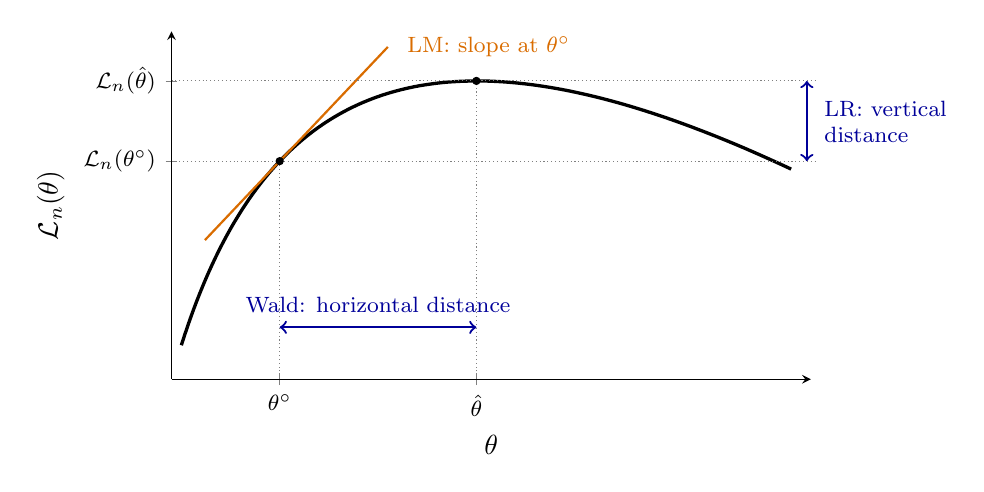
\begin{tikzpicture}
\begin{axis}[
  width=0.8\textwidth, height=6cm,
  xmin=0.45, xmax=3.7, ymin=-4.1, ymax=-0.75,
  axis lines=left, xlabel={$\theta$}, ylabel={$\mathcal{L}_n(\theta)$},
  xtick={1, 2}, xticklabels={$\theta^\circ$, $\hat\theta$},
  ytick={-2, -1.2274}, yticklabels={$\mathcal{L}_n(\theta^\circ)$, $\mathcal{L}_n(\hat\theta)$},
  every tick label/.append style={font=\footnotesize},
  samples=200, domain=0.5:3.6, clip=false]
  \addplot[black, very thick] {4*ln(x) - 2*x};
  \addplot[orange!85!black, thick, domain=0.62:1.55] {-2 + 2*(x - 1)};
  \draw[gray, densely dotted] (axis cs:0.45,-1.2274) -- (axis cs:3.72,-1.2274);
  \draw[gray, densely dotted] (axis cs:0.45,-2) -- (axis cs:3.72,-2);
  \draw[gray, densely dotted] (axis cs:1,-4.1) -- (axis cs:1,-2);
  \draw[gray, densely dotted] (axis cs:2,-4.1) -- (axis cs:2,-1.2274);
  \draw[<->, thick, blue!60!black] (axis cs:3.68,-2) -- (axis cs:3.68,-1.2274);
  \node[font=\footnotesize, anchor=west, text=blue!60!black, align=left] at (axis cs:3.72,-1.62) {LR: vertical\\ distance};
  \draw[<->, thick, blue!60!black] (axis cs:1,-3.6) -- (axis cs:2,-3.6);
  \node[font=\footnotesize, anchor=south, text=blue!60!black, yshift=2pt] at (axis cs:1.5,-3.6) {Wald: horizontal distance};
  \node[font=\footnotesize, anchor=west, text=orange!85!black] at (axis cs:1.6,-0.9) {LM: slope at $\theta^\circ$};
  \fill (axis cs:1,-2) circle (1.5pt);
  \fill (axis cs:2,-1.2274) circle (1.5pt);
\end{axis}
\end{tikzpicture}
\caption[Geometry of the Wald, likelihood ratio and Lagrange multiplier tests]{Geometry of the Wald, likelihood ratio
and Lagrange multiplier tests of $H_0: \theta = \theta^\circ$ for one parameter. The curve is an illustrative
log-likelihood, $\mathcal{L}_n(\theta) = 4\ln\theta - 2\theta$, maximized at $\hat\theta = 2$, with $\theta^\circ = 1$. The
straight segment is the tangent at $\theta^\circ$, whose slope is the score.}
\label{fig:A-trinity}
\end{figure}

The tests differ in what they require. Wald needs only the unrestricted estimate, LM only the restricted one, and LR both.
LM is convenient when the restricted model is easy and the unrestricted one hard, for instance when testing whether a
random coefficient has zero variance starting from logit estimates. Wald is not invariant to how the restriction is
written. Suppose $\hat\theta = 2$ with standard error $0.5$. Writing $H_0$ as $\theta = 1$ gives $\mathcal{W} = (\frac{2 -
1}{0.5})^2 = 4$. Writing it as $\ln\theta = 0$ gives, by the delta method, $\mathcal{W} = (\frac{\ln 2}{0.25})^2 = 7.7$.
Writing it as $\frac{1}{\theta} = 1$ gives $\mathcal{W} = (\frac{0.5}{0.125})^2 = 16$. The likelihood ratio is the same for
all three, because it depends only on the values of the likelihood. In the normal linear regression the three satisfy
$\mathcal{W} \ge \mathcal{LR} \ge \mathcal{LM}$ in every sample \citep{BerndtSavin1977}.

A likelihood ratio test from the book illustrates the mechanics. \citet{PorterZona1993} estimate a ranked logit model of
bids, described in \cref{sec:A-mle-discrete}, three times: on all bid ranks, on the lowest bids only, and on the higher
ranks only.\footnote{We read NBER Working Paper 4013 (March 1992), the working-paper version of \citet{PorterZona1993}.
Table numbers refer to that version.} If the same coefficients govern both parts, the restricted log-likelihood is the
all-ranks value and the unrestricted one is the sum of the two separate values. For competitive firms the log-likelihoods
are $-291.4$, $-89.85$ and $-199.4$ (WP Table 5), so
\begin{equation*}
  \mathcal{LR} = 2\big[(-89.85) + (-199.4) - (-291.4)\big] = 4.3,
\end{equation*}
with six degrees of freedom and a $p$-value of 0.64 (our computation). For cartel members the values are $-73.97$,
$-44.58$ and $-24.92$ (WP Table 6), so $\mathcal{LR} = 8.94$ with four degrees of freedom and a $p$-value of 0.063. Porter and
Zona reject the null of no phantom bidding for the cartel at about the 10 percent level, and they do not reject it for
the competitive firms (\cref{ch:collusion-evidence}).

\Cref{tab:A-tests} collects the tests used in this book.

\begin{table}[htbp]
\centering
\caption{Specification and hypothesis tests used in this book}
\label{tab:A-tests}
\footnotesize
\renewcommand{\arraystretch}{1.15}
\begin{tabularx}{\textwidth}{@{}>{\raggedright\arraybackslash}p{2.1cm}>{\raggedright\arraybackslash}X
>{\raggedright\arraybackslash}p{1.9cm}>{\raggedright\arraybackslash}p{2.2cm}>{\raggedright\arraybackslash}X@{}}
\toprule
Test & Statistic & Null distribution & Estimates needed & Example in the book \\
\midrule
Wald & $n\,a(\hat\theta)^\T[\hat A\hat V\hat A^\T]^{-1}a(\hat\theta)$ & $\chi^2_r$ & unrestricted & equal sugar demand
coefficients across seasons (\cref{ch:conduct}) \\
Likelihood ratio & $2n[\mathcal{L}_n(\hat\theta) - \mathcal{L}_n(\tilde\theta)]$ & $\chi^2_r$ & both & stability of ranked-logit
coefficients across bid ranks (\cref{ch:collusion-evidence}) \\
Lagrange multiplier & $n\,\bar s_n(\tilde\theta)^\T\tilde{\mathcal{I}}^{-1}\bar s_n(\tilde\theta)$ & $\chi^2_r$ & restricted &
zero variance of a random coefficient from logit estimates (\cref{ch:blp}) \\
Hansen $J$ & $n\,\bar g_n(\hat\theta)^\T\hat S^{-1}\bar g_n(\hat\theta)$ & $\chi^2_{L-K}$ & efficient GMM &
overidentifying restrictions in logit and RC logit demand (\cref{app:problems}) \\
Hausman & $(\hat\beta_C - \hat\beta_E)^\T[\hat V_C - \hat V_E]^{-}(\hat\beta_C - \hat\beta_E)$ & $\chi^2$, d.f.\ = rank
of $V_C - V_E$ & efficient and robust & exogeneity of route share and concentration (\cref{ch:airlines}) \\
Anderson-Rubin & $F$ test of $Z$ in a regression of $y - X\beta^\circ$ on $Z$ & $F(L, n - L - K_1)$ under normality &
none & weak-instrument robust confidence sets (\cref{sec:A-weakiv}) \\
First-stage $F$ & $F$ test of excluded instruments in the first stage & noncentral $F$ & first stage & instrument
strength in demand estimation (\cref{sec:A-weakiv}) \\
Cox & centered $\mathcal{LR}$ between non-nested models, standardized & $N(0, 1)$ & both models & collusion against
Bertrand pricing in 1955 autos (\cref{ch:discrete}) \\
Vuong & $\frac{\sqrt{n}\,\overline{LR}}{\hat\omega}$ & $N(0, 1)$ & both models & choosing between non-nested demand or
conduct models \\
Conditional Kolmogorov & $\max_j\sqrt{n}\,\lvert H_n(Z_j) - F_n(Z_j, \hat\theta)\rvert$ & parametric bootstrap &
parametric model & Gamma-Weibull bid distributions in timber auctions (\cref{ch:auction-empirics}) \\
\bottomrule
\end{tabularx}
\par\smallskip
\parbox{\linewidth}{\footnotesize Notes: $r$ is the number of restrictions, $L$ the number of moments and $K$ the number of
parameters. Subscripts $C$ and $E$ denote an estimator consistent under both hypotheses and one efficient under the null. The
superscript $-$ denotes a generalized inverse. In the Anderson-Rubin row, $L$ counts the excluded instruments and $K_1$
the exogenous regressors partialled out.
$\overline{LR}$ is the average pointwise log-likelihood ratio and $\hat\omega$ its standard deviation
(\cref{sec:A-nonnested}). $H_n$ and $F_n$ are defined in \cref{sec:A-ck-test}.}
\end{table}

\subsection{Likelihoods for discrete outcomes}\label{sec:A-mle-discrete}

\casehead{Binary choice}
Let a latent index $y_i^* = x_i^\T\beta + \varepsilon_i$ determine the outcome $y_i = \indic\{y_i^* > 0\}$, with $\varepsilon_i$
independent of $x_i$ and symmetric with distribution function $F$. Then $\Pr(y_i = 1 \mid x_i) = F(x_i^\T\beta)$, and
\begin{equation*}
  \mathcal{L}_n(\beta) = \frac{1}{n}\sum_{i=1}^n\Big[y_i\ln F(x_i^\T\beta) + (1 - y_i)\ln\{1 - F(x_i^\T\beta)\}\Big].
\end{equation*}
The \emph{logit} takes $F = \Lambda$ with $\Lambda(v) = \frac{e^v}{1 + e^v}$, and the \emph{probit} takes $F = \Phi$, the
standard normal distribution function. Only $\frac{\beta}{\sigma_\varepsilon}$ is identified, so the scale of $\varepsilon$ is
normalized (\cref{sec:A-models}). For the logit, $\Lambda'(v) = \Lambda(v)\{1 - \Lambda(v)\}$, so the score and the
Hessian are
\begin{equation}\label{eq:A-logit-score}
  \nabla_\beta\mathcal{L}_n = \frac{1}{n}\sum_i\{y_i - \Lambda(x_i^\T\beta)\}x_i,
  \qquad
  \nabla_{\beta\beta}\mathcal{L}_n = -\frac{1}{n}\sum_i\Lambda(x_i^\T\beta)\{1 - \Lambda(x_i^\T\beta)\}x_ix_i^\T.
\end{equation}

\begin{proposition}[Concavity of the logit likelihood]\label{prop:A-logit-concave}
If $\sum_ix_ix_i^\T$ is positive definite, the binary logit log-likelihood is strictly concave in $\beta$. Hence it has at
most one maximizer, and any solution of the first-order condition is the ML estimator.
\end{proposition}

\begin{proof}
Each weight $\Lambda(1 - \Lambda)$ in \eqref{eq:A-logit-score} lies in $(0, \frac{1}{4}]$. For any $c \ne 0$,
\begin{equation*}
  c^\T\nabla_{\beta\beta}\mathcal{L}_n\,c = -\frac{1}{n}\sum_i\Lambda_i(1 - \Lambda_i)(x_i^\T c)^2 < 0,
\end{equation*}
because $x_i^\T c \ne 0$ for some $i$ when $\sum_ix_ix_i^\T$ is positive definite. A strictly concave function has at most one
maximizer, and a stationary point of a concave function is a global maximizer.
\end{proof}

A maximizer can fail to exist. If some linear combination of the regressors separates the ones from the zeros perfectly,
the likelihood rises without bound along that direction. The probit log-likelihood is also concave, because $\Phi$ and
$1 - \Phi$ are log-concave. \Cref{thm:A-concave} then gives consistency without compactness.

\casehead{Multinomial and conditional logit}
Let consumer $i$ choose one of $J + 1$ alternatives with utilities $u_{ij} = x_{ij}^\T\beta + \epsilon_{ij}$ and $\epsilon_{ij}$
i.i.d.\ type-I extreme value. With $d_{ij} = 1$ if $i$ chooses $j$, the conditional logit of \citet{McFadden1974} has
\begin{equation*}
  P_{ij}(\beta) = \frac{e^{x_{ij}^\T\beta}}{\sum_{k=0}^Je^{x_{ik}^\T\beta}}, \qquad
  \mathcal{L}_n(\beta) = \frac{1}{n}\sum_i\sum_jd_{ij}\ln P_{ij}(\beta).
\end{equation*}
Using $\frac{\partial\ln P_{ij}}{\partial\beta} = x_{ij} - \bar x_i$ with $\bar x_i = \sum_kP_{ik}x_{ik}$,
\begin{equation*}
  \nabla_\beta\mathcal{L}_n = \frac{1}{n}\sum_i\sum_jd_{ij}(x_{ij} - \bar x_i), \qquad
  \nabla_{\beta\beta}\mathcal{L}_n = -\frac{1}{n}\sum_i\sum_jP_{ij}(x_{ij} - \bar x_i)(x_{ij} - \bar x_i)^\T.
\end{equation*}
The Hessian is minus a weighted covariance matrix, so the log-likelihood is concave. With consumer-level data in many
markets, product-market constants $\delta_{jt}$ can be estimated by ML along with the taste-heterogeneity parameters. They
absorb the unobserved quality $\xi_{jt}$. The mean price coefficient is then recovered in a second step,
$\delta_{jt} = x_{jt}\beta - \alpha p_{jt} + \xi_{jt}$, which still needs instruments (\cref{ch:logit,ch:blp}). This is a
two-step estimator in the sense of \cref{sec:A-twostep}.

\casehead{Binomial entry}
\citet{AtheyLevinSeira2011} model the entry of loggers into Forest Service timber auctions. Each of $N_{L,t}$ potential
loggers enters sale $t$ independently with probability $p_L(X_t, N_t) = \Lambda(X_t\alpha_X + N_t\alpha_N)$, where $X_t$ are
sale characteristics and $N_t$ the numbers of potential entrants. The number of entrants is then
$n_{L,t} \sim \mathrm{Binomial}(N_{L,t}, p_L(X_t, N_t))$, and
\begin{equation*}
  \ln L(\alpha) = \sum_t\Big[n_{L,t}\ln p_L(X_t, N_t) + (N_{L,t} - n_{L,t})\ln\{1 - p_L(X_t, N_t)\}\Big] + \text{const}.
\end{equation*}
This is a grouped logit. The score is $\sum_t\{n_{L,t} - N_{L,t}p_L(X_t, N_t)\}(X_t, N_t)^\T$ and the log-likelihood is
concave. They estimate it on $N = 339$ Northern and $N = 382$ California observations. The coefficient on the number of
active loggers is $-0.041$ (0.006) in the North and $-0.050$ (0.007) in California (Table IV). More potential entrants
lower each one's entry probability, as a mixed-strategy entry equilibrium predicts (\cref{ch:auction-empirics}).

\casehead{Rank-ordered logit}
Sometimes we observe a full ranking of alternatives, such as the order of all bids in a procurement auction. Let
$U_j = V_j + \epsilon_j$ with $\epsilon_j$ i.i.d.\ type-I extreme value, $j = 1, \dots, J$.

\begin{proposition}[Rank-ordered logit]\label{prop:A-exploded-logit}
The probability of the ranking $U_{r_1} > U_{r_2} > \dots > U_{r_J}$ is
\begin{equation}\label{eq:A-exploded}
  \Pr(U_{r_1} > U_{r_2} > \dots > U_{r_J}) = \prod_{m=1}^{J}\frac{e^{V_{r_m}}}{\sum_{k=m}^Je^{V_{r_k}}}.
\end{equation}
\end{proposition}

\begin{proof}
The type-I extreme value distribution function is $\Pr(\epsilon \le a) = \exp(-e^{-a})$. Hence $E_j = e^{-\epsilon_j}$ is
exponential with rate one, since $\Pr(e^{-\epsilon_j} > t) = \Pr(\epsilon_j < -\ln t) = e^{-t}$. Define
$T_j = e^{-U_j} = e^{-V_j}E_j$, which is exponential with rate $\lambda_j = e^{V_j}$. The map $u \mapsto e^{-u}$ is
decreasing, so the ranking of the $U$'s from highest to lowest is the ranking of the $T$'s from smallest to largest. For
independent exponentials, $\Pr(T_{r_1} = \min_kT_k) = \frac{\lambda_{r_1}}{\sum_k\lambda_k}$. By the memoryless property, given
that $T_{r_1}$ is the minimum, the excesses $T_k - T_{r_1}$ for $k \ne r_1$ are again independent exponentials with rates
$\lambda_k$, independent of $T_{r_1}$. The ordering of the remaining $T$'s equals the ordering of these excesses, so the
argument repeats on the remaining set. Multiplying the stage probabilities gives \eqref{eq:A-exploded}, with
$\lambda_{r_m} = e^{V_{r_m}}$.
\end{proof}

The ranking likelihood ``explodes'' into a sequence of logit choices from shrinking choice sets
\citep{BeggsCardellHausman1981}. Each auction contributes one product \eqref{eq:A-exploded}, and the sample likelihood is
the product over auctions. Standard multinomial logit software estimates it.

\citet{PorterZona1993} apply the model to bids for highway paving contracts on Long Island, 1979--1985. They approximate the equilibrium bid
function by $\log b_{it} = \alpha_t + X_{it}\beta + \epsilon_{it}$, with an auction effect $\alpha_t$ and an auction-specific
error variance $\sigma_t^2$. They deflate the data by the estimated $\sigma_t$. The probability that firm $i$ submits the
lowest bid is then a multinomial logit in the deflated cost shifters $Z_{it}$, in which the auction effect cancels:
\begin{equation*}
  \Pr(b_{it} < b_{jt}\ \forall j \ne i) = \frac{e^{\beta Z_{it}}}{\sum_je^{\beta Z_{jt}}}.
\end{equation*}
The low bid is the ``most preferred'' alternative, so with $r_m$ the firm whose bid is ranked $m$-th lowest among $n_t$ bids,
\eqref{eq:A-exploded} gives the likelihood $L(\beta) = \prod_t\prod_{i=1}^{n_t}\frac{e^{\beta Z_{r_it}}}{\sum_{j=i}^{n_t}e^{\beta Z_{r_jt}}}$.
The model follows from the bid equation if minus the bid error is type-I extreme value (WP pp.~24--25). The product splits
into the factor for the lowest bid ($i = 1$) and the factors for the higher ranks ($i \ge 2$). Under the model both parts
identify the same $\beta$. Phantom bids by cartel members, placed above the designated winner's bid, need not reflect costs.
The likelihood ratio test of equal coefficients computed above therefore detects them, with the competitive firms as a
check on the specification \citep{HausmanRuud1987}.

\subsection{Latent variables}\label{sec:A-mle-latent}

Many IO models contain variables that the firms observe and the econometrician does not: an auction-level shock common
to all bidders, or the regime of a cartel. The likelihood of the data integrates the latent variable out,
\begin{equation*}
  f(y \mid x;\theta) = \int f(y \mid x, u;\theta)\,\dd F(u \mid x;\theta).
\end{equation*}
Three cases arise in this book: an integral with a closed form, a finite mixture, and a hidden Markov chain.

\subsubsection*{Closed-form heterogeneity: Gamma-Weibull bids}

\citet{AtheyLevinSeira2011} find that sealed bids in the same timber auction are highly correlated given observed sale
characteristics. Following \citet{Krasnokutskaya2011}, they let an auction characteristic $u$, known to the bidders but not
to the econometrician, shift all bids. Conditional on $(X, u, N, n)$, the bid of a bidder of type $k \in \{L, M\}$ (logger or
mill) is Weibull (journal p.~237, eq.~8):
\begin{equation}\label{eq:A-weibull}
  G_k(b \mid X, u, N, n) = 1 - \exp\left\{-u\left(\frac{b}{\lambda_k(X, N, n)}\right)^{\rho_k(n)}\right\}.
\end{equation}
The scale satisfies $\ln\lambda_k = X\beta_X + N\beta_N + n\beta_{n,k} + \beta_{0,k}$ and the shape satisfies
$\ln\rho_k = n\gamma_{n,k} + \gamma_{0,k}$. The heterogeneity $u$ is Gamma with mean one and variance $\sigma_u^2$,
independent of $(X, N, n)$. Athey, Levin and Seira (ALS) denote this variance by $\theta$. Bids are independent given $u$. A large $u$ lowers every
bid in the auction by the common factor $u^{-\frac{1}{\rho_k}}$, since \eqref{eq:A-weibull} says that $u^{\frac{1}{\rho_k}}b$
is Weibull with parameters $(\lambda_k, \rho_k)$ whatever $u$ is.

\begin{proposition}[Closed-form auction likelihood]\label{prop:A-gamma-weibull}
Let auction $t$ have the set of participants $\mathcal{N}_t$, with $\lvert\mathcal{N}_t\rvert = n$ bids $b_i$, and write
$z_i = (\frac{b_i}{\lambda_{k(i)}})^{\rho_{k(i)}}$. The joint density of the bids is
\begin{equation}\label{eq:A-gw-lik}
  \ell_t = \prod_{i \in \mathcal{N}_t}\left[\frac{\rho_{k(i)}}{\lambda_{k(i)}}\left(\frac{b_i}{\lambda_{k(i)}}\right)^{\rho_{k(i)} - 1}\right]
  \frac{\Gamma\big(n + \frac{1}{\sigma_u^2}\big)}{\Gamma\big(\frac{1}{\sigma_u^2}\big)\,
  \big(\sigma_u^2\big)^{\frac{1}{\sigma_u^2}}\,\big(\sum_{i \in \mathcal{N}_t}z_i + \frac{1}{\sigma_u^2}\big)^{n + \frac{1}{\sigma_u^2}}}.
\end{equation}
\end{proposition}

\begin{proof}
Differentiating \eqref{eq:A-weibull}, the density of one bid given $u$ is
\begin{equation*}
  g_k(b \mid u) = u\,\frac{\rho_k}{\lambda_k}\left(\frac{b}{\lambda_k}\right)^{\rho_k - 1}e^{-uz}, \qquad
  z = \left(\frac{b}{\lambda_k}\right)^{\rho_k}.
\end{equation*}
Given $u$ the bids are independent, so their joint density is
\begin{equation*}
  u^{n}\prod_{i \in \mathcal{N}_t}\left[\frac{\rho_{k(i)}}{\lambda_{k(i)}}\left(\frac{b_i}{\lambda_{k(i)}}\right)^{\rho_{k(i)} -
  1}\right]\exp\Big(-u\sum_{i \in \mathcal{N}_t}z_i\Big).
\end{equation*}
A Gamma variable with mean one and variance $\sigma_u^2$ has shape $a = \frac{1}{\sigma_u^2}$, scale
$\sigma_u^2$, and density $\frac{u^{a-1}e^{-\frac{u}{\sigma_u^2}}}{\Gamma(a)(\sigma_u^2)^a}$. Integrating $u$ out leaves
\begin{equation*}
  \frac{1}{\Gamma(a)(\sigma_u^2)^a}\int_0^\infty u^{n + a - 1}
  \exp\left\{-u\left(\sum_iz_i + \frac{1}{\sigma_u^2}\right)\right\}\dd u
  = \frac{\Gamma(n + a)}{\Gamma(a)(\sigma_u^2)^a\big(\sum_iz_i + \frac{1}{\sigma_u^2}\big)^{n + a}},
\end{equation*}
by the Gamma integral $\int_0^\infty u^{c-1}e^{-du}\,\dd u = \frac{\Gamma(c)}{d^c}$. Multiplying by the product term gives
\eqref{eq:A-gw-lik}.
\end{proof}

The Gamma mixing distribution is conjugate to the exponential kernel in \eqref{eq:A-weibull}, which is why the integral has a
closed form. ALS write their likelihood in an online appendix (journal p.~238). The expression above is our derivation
from their specification. They estimate it on sales with at least two bidders (Table IV notes). The estimates of
$\ln\sigma_u^2$ are $-0.502$ (0.120) in the Northern sales and $-0.416$ (0.124) in California (Table IV). These imply
$\sigma_u^2 = 0.61$ and $0.66$, with delta-method standard errors of 0.07 and 0.08 (our computation). Auction
heterogeneity is substantial. The fitted model reproduces the moments of normalized bids. In the North the data show a
mean of 2.16, a standard deviation of 1.18, a between-auction standard deviation of 0.94 and a within-auction standard
deviation of 0.75. The model predicts 2.12, 1.21, 0.97 and 0.70 (journal p.~238). When no conjugate pair exists, the
integral is computed by quadrature or simulation (\cref{sec:A-simulation}).

\subsubsection*{Finite mixtures and switching regressions: the JEC cartel}

\citet{Porter1983} studies the Joint Executive Committee (JEC), a legal railroad cartel that set rates for grain shipped
east from Chicago. The data are weekly from 1880 to 1886, 328 observations. The cartel alternated between collusive
periods and price wars, and the econometrician does not know with certainty which weeks were which. Let $Q_t$ be the
tonnage shipped, $p_t$ the grain rate and $L_t$ a dummy for the Great Lakes being open to navigation. Let $S_t$ collect
dummies for entry and acquisitions and $I_t$ indicate the collusive regime. The model is (journal pp.~304--305)
\begin{align}
  \log Q_t &= \alpha_0 + \alpha_1\log p_t + \alpha_2L_t + U_{1t},\label{eq:A-porter-demand}\\
  \log p_t &= \beta_0 + \beta_1\log Q_t + \beta_2S_t + \beta_3I_t + U_{2t}.\label{eq:A-porter-supply}
\end{align}
The errors $U_t = (U_{1t}, U_{2t})^\T$ are i.i.d.\ $N(0, \Sigma)$. Twelve four-week seasonal dummies enter both equations
and are suppressed here. The regime shifts only the intercept of the supply relation. Porter derives
\eqref{eq:A-porter-supply} from firm first-order conditions $p_t(1 + \frac{\theta_t}{\alpha_1}) = MC_i(q_{it})$. If price wars
are Bertrand and collusive periods have constant conduct $\theta$, then $\beta_3 = -\ln(1 + \frac{\theta}{\alpha_1})$.

Write the system as $By_t = \Gamma X_t + \Delta I_t + U_t$ with $y_t = (\log Q_t, \log p_t)^\T$, $X_t = (1, L_t, S_t^\T)^\T$ and
\begin{equation*}
  B = \begin{pmatrix} 1 & -\alpha_1 \\ -\beta_1 & 1\end{pmatrix}, \qquad
  \Delta = \begin{pmatrix} 0 \\ \beta_3\end{pmatrix}, \qquad
  \Gamma = \begin{pmatrix} \alpha_0 & \alpha_2 & 0 \\ \beta_0 & 0 & \beta_2^\T\end{pmatrix}.
\end{equation*}
Given $I_t$, the change of variables from $U_t$ to $y_t$ has Jacobian $\lvert\det B\rvert = \lvert 1 - \alpha_1\beta_1\rvert$, so
\begin{equation}\label{eq:A-porter-h}
  h(y_t \mid I_t) = (2\pi)^{-1}\lvert\Sigma\rvert^{-\frac{1}{2}}\lvert\det B\rvert
  \exp\left\{-\frac{1}{2}(By_t - \Gamma X_t - \Delta I_t)^\T\Sigma^{-1}(By_t - \Gamma X_t - \Delta I_t)\right\}.
\end{equation}
If the regimes are known, 2SLS or ML with $I_t$ as data is straightforward. Porter instead treats $I_t$ as an i.i.d.
Bernoulli variable with $\Pr(I_t = 1) = \lambda$. The density of $y_t$ is then a two-component mixture, and the likelihood is
(journal p.~306, eq.~5)
\begin{equation}\label{eq:A-mixture}
  L(\Omega, \lambda) = \prod_{t=1}^T\big[\lambda h(y_t \mid 1) + (1 - \lambda)h(y_t \mid 0)\big],
\end{equation}
with $\Omega = (B, \Gamma, \Delta, \Sigma)$.

Mixture likelihoods are awkward to maximize directly, because the log of a sum does not separate. The
\emph{expectation-maximization} (EM) algorithm of \citet{DempsterLairdRubin1977} exploits the fact that the likelihood
would be easy if the regimes were observed. The complete-data log-likelihood is
\begin{equation*}
  \ln L^c(\Omega, \lambda) = \sum_t\Big[I_t\{\ln\lambda + \ln h(y_t \mid 1)\} + (1 - I_t)\{\ln(1 - \lambda) + \ln h(y_t \mid 0)\}\Big].
\end{equation*}
Starting from $(\Omega^{(m)}, \lambda^{(m)})$, iterate two steps.
\begin{enumerate}
  \item \emph{E step.} Compute the posterior probability of collusion in each week by Bayes' rule,
  \begin{equation}\label{eq:A-estep}
    w_t^{(m)} = \Pr(I_t = 1 \mid y_t;\Omega^{(m)}, \lambda^{(m)}) =
    \frac{\lambda^{(m)}h(y_t \mid 1;\Omega^{(m)})}{\lambda^{(m)}h(y_t \mid 1;\Omega^{(m)}) + (1 - \lambda^{(m)})h(y_t \mid 0;\Omega^{(m)})}.
  \end{equation}
  \item \emph{M step.} Maximize the expected complete-data log-likelihood, which replaces $I_t$ by $w_t^{(m)}$ in
  $\ln L^c$. This gives $\lambda^{(m+1)} = \frac{1}{T}\sum_tw_t^{(m)}$ and
  \begin{equation*}
    \Omega^{(m+1)} = \argmax_\Omega\sum_t\Big[w_t^{(m)}\ln h(y_t \mid 1;\Omega) + (1 - w_t^{(m)})\ln h(y_t \mid 0;\Omega)\Big],
  \end{equation*}
  a weighted full-information ML problem.
\end{enumerate}
Porter adapts the version of this algorithm proposed by \citet{Kiefer1980} for switching regressions. He stops when the
correlation between successive $w_t$ series exceeds .999 (journal p.~306).

A detail of the M step deserves care. The weighted objective is not the known-regime likelihood with $w_t$ substituted for
$I_t$. Write $e_t = By_t - \Gamma X_t$. The expected complete-data log-likelihood weights the quadratic forms of the two
regimes by $w_t$ and $1 - w_t$, and completing the square gives
\begin{equation*}
  w_t(e_t - \Delta)^\T\Sigma^{-1}(e_t - \Delta) + (1 - w_t)e_t^\T\Sigma^{-1}e_t
  = (e_t - w_t\Delta)^\T\Sigma^{-1}(e_t - w_t\Delta) + w_t(1 - w_t)\Delta^\T\Sigma^{-1}\Delta.
\end{equation*}
The plug-in shortcut drops the last term, which matters when posterior probabilities are far from zero and one. In the
simulated example below, the shortcut converges to $\hat\beta_3 = 0.618$, with a mixture log-likelihood 5.7 points below the
maximum attained by exact EM.

\begin{proposition}[EM never lowers the likelihood]\label{prop:A-em-monotone}
Let $\vartheta = (\Omega, \lambda)$ and let $\vartheta^{(m+1)}$ maximize
$\mathcal{Q}(\vartheta \mid \vartheta^{(m)}) = \E[\ln L^c(\vartheta) \mid y;\vartheta^{(m)}]$. Then
$\ln L(\vartheta^{(m+1)}) \ge \ln L(\vartheta^{(m)})$.
\end{proposition}

\begin{proof}
Let $k(I \mid y;\vartheta)$ be the conditional probability of the regime sequence $I$ given the data. By the definition of
conditional probability, $\ln L(\vartheta) = \ln L^c(\vartheta) - \ln k(I \mid y;\vartheta)$ for every $I$. Take the expectation
over $I$ under $k(\cdot \mid y;\vartheta^{(m)})$. The left side does not depend on $I$, so
\begin{equation*}
  \ln L(\vartheta) = \mathcal{Q}(\vartheta \mid \vartheta^{(m)}) - \mathcal{H}(\vartheta \mid \vartheta^{(m)}),
  \qquad
  \mathcal{H}(\vartheta \mid \vartheta^{(m)}) = \E[\ln k(I \mid y;\vartheta) \mid y;\vartheta^{(m)}].
\end{equation*}
By \cref{lem:A-info-inequality} applied to the conditional distribution of $I$, $\mathcal{H}(\vartheta \mid \vartheta^{(m)}) \le
\mathcal{H}(\vartheta^{(m)} \mid \vartheta^{(m)})$ for every $\vartheta$. The M step gives $\mathcal{Q}(\vartheta^{(m+1)} \mid
\vartheta^{(m)}) \ge \mathcal{Q}(\vartheta^{(m)} \mid \vartheta^{(m)})$. Hence
\begin{align*}
  \ln L(\vartheta^{(m+1)}) - \ln L(\vartheta^{(m)})
  &= \big[\mathcal{Q}(\vartheta^{(m+1)} \mid \vartheta^{(m)}) - \mathcal{Q}(\vartheta^{(m)} \mid \vartheta^{(m)})\big] \\
  &\quad - \big[\mathcal{H}(\vartheta^{(m+1)} \mid \vartheta^{(m)}) - \mathcal{H}(\vartheta^{(m)} \mid \vartheta^{(m)})\big]
  \ge 0. \qedhere
\end{align*}
\end{proof}

The proof also shows that the gradient of $\mathcal{H}(\cdot \mid \vartheta^{(m)})$ is zero at $\vartheta^{(m)}$. So a fixed point
of EM is a stationary point of the observed likelihood. It need not be the global maximum. Convergence is linear, and slow
when the regimes carry much missing information. EM does not deliver standard errors. They come from the observed
information of the mixture likelihood \eqref{eq:A-mixture} at the EM solution \citep{Louis1982}.

After estimation each week is classified as collusive if $\hat w_t > .5$. The rule minimizes the expected number of
misclassified weeks \citep{LeePorter1984}. The expected number of errors of a classification $\hat I_t$ is
$\sum_t[\hat I_t(1 - \hat w_t) + (1 - \hat I_t)\hat w_t]$, and each term is minimized by choosing $\hat I_t = 1$ exactly when
$\hat w_t > 1 - \hat w_t$.

Porter compares 2SLS with a regime series reported in the trade press (the PO series) and ML with the estimated series (PN).
The demand estimates are almost identical, with price elasticities of $-.742$ (.121) and $-.800$ (.091). The regime
coefficient $\hat\beta_3$ rises from .382 (.059) under 2SLS to .545 (.032) under ML. It is larger and has about half the
standard error. The $R^2$ of the supply relation rises from .320 to .863 (Table 3). The implied conduct parameter is
\begin{equation*}
  \hat\theta = \hat\alpha_1\big(e^{-\hat\beta_3} - 1\big) = -0.800\times\big(e^{-0.545} - 1\big) = 0.336,
\end{equation*}
which Porter calls roughly consistent with Cournot behavior in collusive periods (journal p.~309). At sample means,
collusive weeks have prices about 66 percent higher, quantities about 33 percent lower and revenues about 11 percent
higher than price-war weeks (Table 4, p.~310). The full table and its interpretation are in \cref{ch:collusion-evidence}.

\Cref{fig:A-em} applies the algorithm to simulated data with the same structure. Demand and supply parameters are set near
Porter's ML estimates, and the regime follows a Markov chain with the transition probabilities that \citet{Ellison1994}
estimates. The simulated sample has six price wars covering 65 of 328 weeks. Exact EM from a median split of the supply
residuals converges in 25 iterations to $\hat\beta_3 = 0.563$ (0.030), against the true 0.545. The correlation between
successive $w_t$ series first exceeds .999 at iteration 10. The rule $\hat w_t > .5$ misclassifies 11 weeks. The
log-likelihood rises at every iteration, as \cref{prop:A-em-monotone} requires. A random starting classification shows the
other side of the proposition. It carries no information about the regimes, so the first M step sets $\hat\beta_3$ close to
zero. With equal regime densities every posterior equals $\lambda$, and the algorithm stays at this degenerate fixed point,
37.3 log points below the maximum (\cref{fig:A-em}, panel a).

\begin{figure}[htbp]
\centering
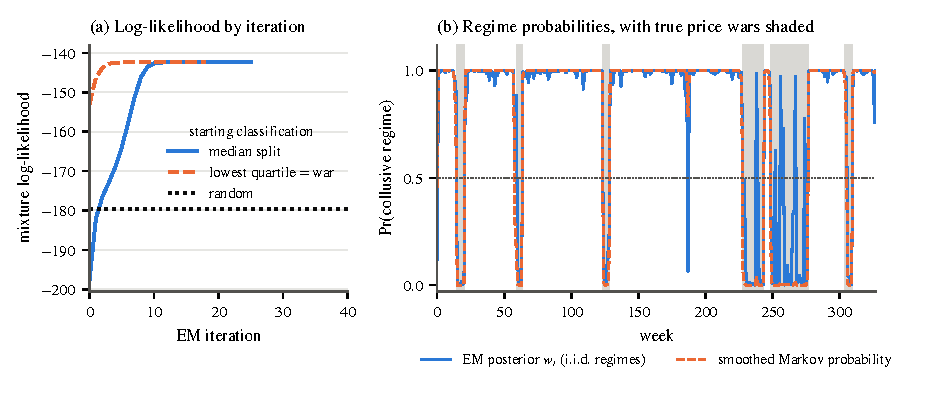
\includegraphics[width=\textwidth]{figures/appA/em_switching.pdf}
\caption[EM and Markov-switching estimation of a simulated two-regime supply relation]{EM and Markov-switching
estimation of a simulated two-regime supply relation. The design is \eqref{eq:A-porter-demand} and
\eqref{eq:A-porter-supply} with $T = 328$, $(\alpha_0, \alpha_1, \alpha_2) = (9.09, -0.80, -0.43)$, $(\beta_0, \beta_1, \beta_2, \beta_3) = (-2.70, 0.09,
-0.20, 0.545)$, one entry dummy, independent errors with standard deviations 0.40 and 0.16, and a Markov regime with
$\Pr(I_{t+1} = 1 \mid I_t = 1) = 0.975$ and $\Pr(I_{t+1} = 1 \mid I_t = 0) = 0.067$. (a) Mixture log-likelihood
by EM iteration from three starting classifications. (b) Posterior probabilities of collusion from the i.i.d.
mixture (EM) and smoothed probabilities from the Markov-switching model estimated by the Hamilton filter. Source:
\texttt{figures/appA/src/em\_switching.py}, seed 20261022.}
\label{fig:A-em}
\end{figure}

\subsubsection*{Hidden Markov models: Ellison's re-estimation}

Porter's i.i.d.\ regimes ignore the persistence of price wars. \citet{Ellison1994} re-estimates the JEC model with two
changes (journal p.~40). First, the demand error follows an AR(1) process, $U_{1t} = \rho U_{1,t-1} + V_{1t}$ with
$\lvert\rho\rvert < 1$, where $\rho$ now denotes an autoregressive coefficient. Second, the regime follows a Markov chain whose
transition probabilities are logits,
\begin{equation}\label{eq:A-ellison-transition}
  \Pr(I_{t+1} = 1 \mid I_t, Z_t) = \frac{e^{\gamma^\T W_t}}{1 + e^{\gamma^\T W_t}},
\end{equation}
where $Z_t$ is the set of predetermined variables at $t$ and $W_t$ contains functions of $I_t$ and of $Z_t$. With $W_t$
equal to a separate constant for each value of $I_t$, the chain is a first-order Markov process. Adding market-share or
demand variables to $W_t$ tests what triggers price wars. Ellison maximizes the joint likelihood of the structural
equations and of the path of transitions.

The likelihood of a hidden Markov model is computed by the filter of \citet{Hamilton1989}. Let $\mathcal{F}_t$ be the data
up to week $t$, and let $h_k(y_t) = f(y_t \mid I_t = k, \mathcal{F}_{t-1})$ be the density of week $t$'s data in regime $k$.
In Ellison's model, $h_k$ is \eqref{eq:A-porter-h} with $U_{1t}$ replaced by $V_{1t} = U_{1t} - \rho U_{1,t-1}$. Write
$p_{k,t} = \Pr(I_{t+1} = 1 \mid I_t = k, Z_t)$, the predicted probability $\xi_{t \mid t-1} = \Pr(I_t = 1 \mid \mathcal{F}_{t-1})$,
and the filtered probability $\xi_{t \mid t} = \Pr(I_t = 1 \mid \mathcal{F}_t)$.

\begin{proposition}[Hamilton filter]\label{prop:A-hamilton}
Suppose $y_t$ depends on the regime history only through $I_t$, given $\mathcal{F}_{t-1}$, and the regime follows
\eqref{eq:A-ellison-transition}. Then for $t = 1, \dots, T$,
\begin{align}
  f(y_t \mid \mathcal{F}_{t-1}) &= \xi_{t \mid t-1}h_1(y_t) + (1 - \xi_{t \mid t-1})h_0(y_t),\label{eq:A-ham-pred}\\
  \xi_{t \mid t} &= \frac{\xi_{t \mid t-1}h_1(y_t)}{f(y_t \mid \mathcal{F}_{t-1})},\label{eq:A-ham-update}\\
  \xi_{t+1 \mid t} &= p_{1,t}\,\xi_{t \mid t} + p_{0,t}\,(1 - \xi_{t \mid t}),\label{eq:A-ham-forecast}
\end{align}
and the log-likelihood is $\ln L = \sum_{t=1}^T\ln f(y_t \mid \mathcal{F}_{t-1})$.
\end{proposition}

\begin{proof}
Equation \eqref{eq:A-ham-pred} is the law of total probability over the two values of $I_t$ given $\mathcal{F}_{t-1}$. Equation
\eqref{eq:A-ham-update} is Bayes' rule, $\Pr(I_t = 1 \mid y_t, \mathcal{F}_{t-1}) = \frac{\Pr(I_t = 1 \mid \mathcal{F}_{t-1})
f(y_t \mid I_t = 1, \mathcal{F}_{t-1})}{f(y_t \mid \mathcal{F}_{t-1})}$. Equation \eqref{eq:A-ham-forecast} again applies the law of
total probability, now over $I_t$ given $\mathcal{F}_t$, using that the transition depends on $\mathcal{F}_t$ only through
$(I_t, Z_t)$. Finally, the joint density of $(y_1, \dots, y_T)$ factors into one-step predictive densities,
$f(y_1, \dots, y_T) = \prod_tf(y_t \mid \mathcal{F}_{t-1})$.
\end{proof}

The recursion needs a starting value $\xi_{1 \mid 0}$, usually the stationary probability $\frac{p_0}{1 - p_1 + p_0}$ when the
transition probabilities are constant. Probabilities that use the whole sample come from a backward pass
\citep{Kim1994}:
\begin{equation*}
  \Pr(I_t = 1 \mid \mathcal{F}_T) = \xi_{t \mid t}\left[p_{1,t}\frac{\Pr(I_{t+1} = 1 \mid \mathcal{F}_T)}{\xi_{t+1 \mid t}} +
  (1 - p_{1,t})\frac{\Pr(I_{t+1} = 0 \mid \mathcal{F}_T)}{1 - \xi_{t+1 \mid t}}\right].
\end{equation*}
In the simulated data of \cref{fig:A-em}, the Markov-switching model estimated by maximizing this likelihood gives
$\Pr(I_{t+1} = 1 \mid I_t = 1) = 0.975$ and $\Pr(I_{t+1} = 1 \mid I_t = 0) = 0.099$, against the true 0.975 and 0.067. The
smoothed probabilities misclassify 5 weeks, against 11 for the i.i.d.\ mixture. Using the persistence of regimes sharpens
the classification of short-lived deviations.

Ellison's estimates (Table 2) give regime constants of 3.675 (.474) after a collusive week and $-2.641$ (.404) after a price
war week. A collusive week is followed by another with probability $\frac{e^{3.675}}{1 + e^{3.675}} = .975$. A price war week
is followed by collusion with probability only $\frac{e^{-2.641}}{1 + e^{-2.641}} = .067$, so wars persist with probability
.933 per week. The implied mean durations are about 40 weeks for collusive spells and 15 weeks for wars, and the stationary
share of collusive weeks is .73 (our computation). Dependence also moves the structural estimates. Allowing AR(1) demand
errors, with $\hat\rho = .832$ (.085), raises the estimated demand elasticity from .84 to 1.80 (journal p.~42). Porter's
approximation to the degree of collusion, $\hat\alpha_1(e^{-\hat\beta_3} - 1)$, rises from .40 to .85. The estimated elasticity is
imprecise, with a standard error of 1.29. The log-likelihood rises from 37.2 to 181.0. If both values are computed on the
same 328 weeks, the implied likelihood ratio statistic for $\rho = 0$ is 287.6 (our computation).

Ellison then adds candidate triggers to $W_t$ in the transition from collusion to war (Table 3). An unusually high market
share for one firm (BIGSHARE1) enters with coefficient $-.77$ (.49), and the unanticipated demand shock $V_{1t}$ with $-4.15$
(2.64). Both have the predicted sign and are significant at about the 6 percent level in one-tailed tests. With only six
price wars in the sample, these tests have little power. \Cref{ch:collusion-evidence} discusses what they imply for the
theories of \citet{GreenPorter1984} and \citet{RotembergSaloner1986}. The econometric point is that joint ML of the regimes,
the transitions and the structural equations uses the timing of every war. A two-step procedure that first classifies weeks
and then regresses the classification on triggers may lose power through misclassification at the onset of wars
(journal p.~39).

\subsection{Non-regular problems}\label{sec:A-mle-nonregular}

The standard theory assumes that the support of the data does not depend on $\theta$, that $\theta_0$ is interior, and that
the likelihood is smooth. Each assumption fails in some IO application, and each failure changes the asymptotics.

\begin{proposition}[Parameter-dependent support]\label{prop:A-uniform-mle}
Let $X_1, \dots, X_n$ be i.i.d.\ uniform on $[0, \theta_0]$. The ML estimator is $\hat\theta = \max_iX_i$, and
\begin{equation*}
  \frac{n(\theta_0 - \hat\theta)}{\theta_0} \xrightarrow{d} \mathrm{Exponential}(1).
\end{equation*}
\end{proposition}

\begin{proof}
The likelihood is $\theta^{-n}\indic\{\theta \ge \max_iX_i\}$, which is zero below the sample maximum and decreasing above it.
So $\hat\theta = \max_iX_i$. For $0 \le t \le n$,
\begin{equation*}
  \Pr\left(\frac{n(\theta_0 - \hat\theta)}{\theta_0} > t\right) = \Pr\left(\max_iX_i < \theta_0\left(1 - \frac{t}{n}\right)\right)
  = \left(1 - \frac{t}{n}\right)^n \to e^{-t}. \qedhere
\end{equation*}
\end{proof}

The estimator converges at rate $n$, faster than $\sqrt{n}$, and its limit is not normal. It is biased downward, with
$\E[\hat\theta] = \frac{n}{n + 1}\theta_0$. The information equality fails because the support moves with $\theta$. The
derivative of $\ln f = -\ln\theta$ is $-\frac{1}{\theta}$, whose mean is not zero. The same structure arises in first-price
auctions, where the upper end of the bid support depends on the parameters of the value distribution.
\citet{DonaldPaarsch1996} develop estimators and tests for this case based on extreme order statistics
(\cref{ch:auction-empirics}). \Cref{prop:A-boot-max} shows that the nonparametric bootstrap fails here.

\begin{proposition}[A parameter on the boundary]\label{prop:A-boundary}
Let $\theta$ be scalar with $\Theta = [0, \infty)$ and $\theta_0 = 0$. Suppose the log-likelihood extends smoothly to a
neighborhood of zero, where the unconstrained maximizer $\hat\theta_u$ satisfies $\sqrt{n}\,\hat\theta_u \xrightarrow{d}
N(0, \mathcal{I}^{-1})$. Then the likelihood ratio statistic for $H_0: \theta = 0$ converges in distribution to an equal mixture
of a point mass at zero and a $\chi^2_1$.
\end{proposition}

\begin{proof}
A second-order expansion around zero, with $\bar s_n(0) = \mathcal{I}\hat\theta_u + o_p(n^{-\frac{1}{2}})$, gives uniformly in
$\theta$ of order $n^{-\frac{1}{2}}$,
\begin{equation*}
  2n\big[\mathcal{L}_n(\theta) - \mathcal{L}_n(0)\big] = n\mathcal{I}\big(2\theta\hat\theta_u - \theta^2\big) + o_p(1).
\end{equation*}
Maximize over $\theta \ge 0$. If $\hat\theta_u > 0$ the maximum is at $\theta = \hat\theta_u$, with value $n\mathcal{I}\hat\theta_u^2$.
If $\hat\theta_u \le 0$ the maximum is at $\theta = 0$, with value zero. So $\mathcal{LR} = (\max\{0, Z_n\})^2 + o_p(1)$ with
$Z_n = \sqrt{n\mathcal{I}}\,\hat\theta_u \xrightarrow{d} N(0, 1)$. Half the time $Z_n \le 0$ and the statistic is zero. Otherwise it is
the square of a standard normal.
\end{proof}

The 5 percent cutoff of this mixture is the 90th percentile of $\chi^2_1$, 2.71, not the usual 3.84
\citep{Chernoff1954, SelfLiang1987, Andrews2001}. Zero variances of random coefficients and zero regime probabilities are
boundary nulls of this kind. Testing the number of regimes is harder still. In Porter's model \eqref{eq:A-mixture} the
null of a single regime can be written in two ways. If $\lambda = 0$, then $\lambda$ lies on the boundary and $\beta_3$ is
not identified, because it multiplies a regime that never occurs. The case $\lambda = 1$ is symmetric. Then $I_t = 1$ in every
week, so $\beta_3$ cannot be separated from the intercept $\beta_0$. If $\beta_3 = 0$, the two mixture components coincide,
and $\lambda$ is not identified. In both cases a parameter is identified only under the alternative. The likelihood ratio
then has no $\chi^2$ limit \citep{Davies1977}, and \citet{Hansen1992} develops bounds for Markov-switching models.

Porter's own test shows the problem at work. He maximizes the likelihood once with switching and once subject to
$\Delta = 0$, which in \eqref{eq:A-porter-supply} means $\beta_3 = 0$. Let $\bar L_1$ and $\bar L_0$ be the two maximized
average log-likelihoods. He reports $2T(\bar L_1 - \bar L_0) = 554.1$, refers it to a $\chi^2_1$ distribution, and
rejects ``the hypothesis that no switch occurred'' (journal p.~312). Under $\Delta = 0$ the mixture density
$\lambda h(y_t \mid 1) + (1 - \lambda)h(y_t \mid 0)$ equals $h(y_t \mid 0)$ for every $\lambda$. The restricted
likelihood is therefore flat in $\lambda$, and the unrestricted fit chooses $\lambda$ and $\beta_3$ together. The
statistic is the largest of a family of likelihood ratios indexed by $\lambda$. Its null distribution is stochastically
larger than $\chi^2_1$, and the $\chi^2_1$ reference is invalid. The size of the statistic still settles the question in
practice. The 0.1 percent cutoff of $\chi^2_1$ is 10.83, and 554.1 is about fifty times larger, so the rejection very
likely survives any valid correction. Porter also notes that $\hat\beta_3$ is significantly positive (journal p.~311). A
$t$ test of $\beta_3 = 0$ faces the same difficulty, because it is computed at an estimate $\hat\lambda$ that has no
limit under the null.

A discontinuous likelihood is the third failure. \citet{Bresnahan1987} solves the vertical model for equilibrium prices
and quantities, adds independent normal errors to observed prices and quantities, and maximizes the resulting likelihood
(\cref{sec:06-bres-estimation}). The likelihood jumps when two products swap positions in the quality ordering. The derivative-based expansion of \cref{thm:A-asy-normal}
is unavailable at the jumps. Estimation then relies on derivative-free search, and asymptotic theory requires the true
parameter to lie away from the discontinuities.

\subsection{Non-nested tests}\label{sec:A-nonnested}

Two models are \emph{non-nested} when neither is a special case of the other. Collusion and Bertrand pricing with the same
demand system are an example (\cref{sec:06-bres-cox}). The likelihood ratio does not have a $\chi^2$ distribution in this
case, and its sign alone is uninformative. Two approaches are standard.

Let model $F$ have density $f(y \mid x;\theta)$ and model $G$ density $g(y \mid x;\gamma)$, with ML estimates $\hat\theta$ and
$\hat\gamma$. Write the pointwise log-likelihood ratio as $d_i = \ln f(y_i \mid x_i;\hat\theta) - \ln g(y_i \mid x_i;\hat\gamma)$
and $LR_n = \sum_id_i$.

The test of \citet{Cox1961, Cox1962} takes $F$ as the null. If $F$ is true with parameter $\theta$, the estimator
$\hat\gamma$ converges to a pseudo-true value $\gamma(\theta)$, and $\frac{1}{n}LR_n$ converges to
$\E_\theta[\ln f(y \mid x;\theta) - \ln g(y \mid x;\gamma(\theta))]$. Cox's statistic centers $LR_n$ by a consistent estimate of
this expectation, computed under $F$ at $\hat\theta$, and divides by an estimate of its standard deviation. Under $F$ it is
asymptotically standard normal. A large negative value says that $G$ fits better than $F$ would lead us to expect. The roles
are then reversed. There are four possible outcomes: reject neither, reject one of the two, or reject both. Rejecting both is
informative, because it says that neither model is adequate. \Cref{prop:06-bres-cox} gives the statistic for nonlinear
regressions with normal errors, and \cref{tab:06-bres-cox} reports Bresnahan's tests of conduct in the 1955 automobile market.

The test of \citet{Vuong1989} treats the models symmetrically. It asks which model is closer to the truth in
Kullback-Leibler divergence.

\begin{proposition}[Vuong's model selection test]\label{prop:A-vuong}
Let $\theta^*$ and $\gamma^*$ be the pseudo-true values of the two models. Suppose $\Pr\{f(y \mid x;\theta^*) \ne g(y \mid
x;\gamma^*)\} > 0$, so that the models are strictly non-nested, and let $\hat\omega^2 = \frac{1}{n}\sum_i(d_i - \bar d)^2$ with
$\bar d = \frac{1}{n}LR_n$. Under $H_0: \E[\ln f(y \mid x;\theta^*) - \ln g(y \mid x;\gamma^*)] = 0$ and standard regularity
conditions,
\begin{equation*}
  T_V = \frac{\sqrt{n}\,\bar d}{\hat\omega} \xrightarrow{d} N(0, 1).
\end{equation*}
\end{proposition}

\begin{proof}[Proof sketch]
Let $\bar d^* = \frac{1}{n}\sum_i[\ln f(y_i \mid x_i;\theta^*) - \ln g(y_i \mid x_i;\gamma^*)]$. Expand $\bar d$ around the
pseudo-true values. The first-order term in $\theta$ is $\bar s^f_n(\theta^*)^\T(\hat\theta - \theta^*)$, where $\bar s^f_n$ is the
average score of model $F$. Its expectation at $\theta^*$ is zero because $\theta^*$ maximizes $\E\ln f$. So $\bar s^f_n(\theta^*) =
O_p(n^{-\frac{1}{2}})$, and with $\hat\theta - \theta^* = O_p(n^{-\frac{1}{2}})$ the product is $O_p(n^{-1})$. The same holds for
$\gamma$. Hence $\sqrt{n}\,\bar d = \sqrt{n}\,\bar d^* + o_p(1)$. Under $H_0$, $\bar d^*$ is an average of i.i.d.\ terms with mean
zero and variance $\omega^2 > 0$, the latter by strict non-nestedness. The central limit theorem and $\hat\omega \xrightarrow{p}
\omega$ finish the argument.
\end{proof}

A large positive $T_V$ favors $F$, a large negative one favors $G$, and a value near zero says the data cannot tell the
models apart. If the models overlap, so that $\omega^2 = 0$, the statistic has a different limit, and Vuong gives a separate
procedure. \citet{RiversVuong2002} extend the test to general estimation criteria, including GMM, which makes it usable for
comparing conduct models estimated from moment conditions.

\subsection{Testing a parametric distribution}\label{sec:A-ck-test}

Parametric models of bids or values are convenient, but their shape restrictions drive the results. A specification test
for the whole conditional distribution is then valuable. The Kolmogorov-Smirnov statistic $\sup_y\sqrt{n}\lvert F_n(y) -
F(y;\hat\theta)\rvert$ compares the empirical and fitted distribution functions. With estimated parameters its null
distribution depends on the model, so tables computed for a known $F$ are wrong, and the cutoff must be simulated.

\citet{Andrews1997} extends the idea to a conditional distribution. Let $Z_i = (Y_i, X_i)$, with $Y_i$ the endogenous
outcomes and $X_i$ the exogenous covariates, and let the model specify $F(y \mid x;\theta)$. Define the empirical
distribution function of $Z$ and a semiparametric estimate of it that uses the model for $Y$ given $X$ and the empirical
distribution of $X$:
\begin{equation*}
  H_n(y, x) = \frac{1}{n}\sum_{i=1}^n\indic\{Y_i \le y, X_i \le x\}, \qquad
  F_n(y, x;\theta) = \frac{1}{n}\sum_{i=1}^nF(y \mid X_i;\theta)\indic\{X_i \le x\}.
\end{equation*}
The \emph{conditional Kolmogorov} statistic is $CK_n = \max_{j \le n}\sqrt{n}\,\lvert H_n(Z_j) - F_n(Z_j;\hat\theta)\rvert$. Its
null distribution is obtained by a parametric bootstrap.
\begin{enumerate}
  \item Estimate $\hat\theta$ and compute $CK_n$.
  \item For $b = 1, \dots, B$, draw $Y_i^{*} \sim F(\cdot \mid X_i;\hat\theta)$ for each $i$, holding the covariates fixed.
  Re-estimate $\hat\theta^{*}$ on the simulated sample and compute $CK_n^{*}$.
  \item Reject at level $a$ if $CK_n$ exceeds the $(1 - a)$ quantile of $CK_n^{*1}, \dots, CK_n^{*B}$.
\end{enumerate}
Re-estimating $\theta$ in each replication accounts for the fact that the fitted model is closer to the data than the true
model would be.

\citet[journal p.~241]{AtheyLevinSeira2011} apply the test to their Gamma-Weibull model. The exogenous covariates are the sale
characteristics $(X, N)$ and the endogenous variables are the bids. They cannot reject the parametric specification even at
the 20 percent level, in both the Northern and the California sales. Together with the close fit of the bid moments reported
above, this supports using the fitted bid distributions to recover values and entry costs (\cref{ch:auction-empirics}).

\section{Simulation-based estimation}\label{sec:A-simulation}

The GMM and likelihood theory of \cref{sec:A-gmm,sec:A-mle} assumes that we can evaluate the moment function or the
density at any trial parameter. Many structural models in industrial organization imply moments or likelihoods that
are integrals with no closed form. The market share of a product in a random coefficients model integrates individual logit probabilities over
the distribution of tastes (\cref{ch:blp}). The expected winning bid in a first-price auction is the expected
second-highest value, an integral over the joint distribution of all bidders' values
\citep{LaffontOssardVuong1995}. The expected profit of an entrant integrates over values, rivals and bids
\citep{AtheyLevinSeira2011}. A counterfactual auction outcome is an expectation over simulated auctions
\citep{Asker2010}. This section shows how such integrals are replaced by averages over random draws and what the
replacement does to the properties of the estimator. The answer depends on how the simulated integral enters the
objective. When it enters linearly, as in a moment condition, simulation adds variance but no bias. When it enters
through a nonlinear function, such as a logarithm, it adds bias that vanishes only as the number of draws grows.

Throughout the section $\theta$ is a generic parameter vector, $n$ is the number of observations and $n_s$ is the
number of simulation draws per observation (the notation of \cref{ch:blp}). Several papers write $S$ for $n_s$, and
we translate their formulas.

\subsection{Monte Carlo integration}\label{sec:A-mc-integration}

Let $\nu$ be a random vector with known distribution $F$, which may depend on $\theta$ only through a known
transformation of standardized draws. The target is an expectation
\begin{equation}\label{eq:A-mc-target}
  \phi(\theta) = \E_\nu\bigl[q(\nu;\theta)\bigr] = \int q(\nu;\theta)\,\dd F(\nu),
\end{equation}
for a function $q$ that we can evaluate at any $(\nu, \theta)$. The \emph{Monte Carlo simulator} of $\phi(\theta)$
averages $q$ over $n_s$ independent draws $\nu_1, \dots, \nu_{n_s}$ from $F$:
\begin{equation}\label{eq:A-mc-simulator}
  \tilde\phi(\theta) = \frac{1}{n_s}\sum_{r=1}^{n_s} q(\nu_r;\theta).
\end{equation}

\begin{proposition}[Monte Carlo integration]\label{prop:A-mc}
Suppose $\sigma_q^2(\theta) = \Var_\nu(q(\nu;\theta))$ is finite. Then
\begin{enumerate}[label=(\roman*)]
  \item $\E[\tilde\phi(\theta)] = \phi(\theta)$, so the simulator is unbiased.
  \item $\Var(\tilde\phi(\theta)) = \frac{\sigma_q^2(\theta)}{n_s}$.
  \item $\sqrt{n_s}\,(\tilde\phi(\theta) - \phi(\theta)) \xrightarrow{d} N(0, \sigma_q^2(\theta))$ as $n_s \to \infty$.
\end{enumerate}
The simulation error is $O_p(n_s^{-\frac{1}{2}})$ whatever the dimension of $\nu$.
\end{proposition}

\begin{proof}
The draws are independent and identically distributed, so each term of \eqref{eq:A-mc-simulator} has mean
$\phi(\theta)$ and variance $\sigma_q^2(\theta)$. Linearity of expectation gives (i). Independence gives
\begin{equation*}
  \Var\bigl(\tilde\phi(\theta)\bigr) = \frac{1}{n_s^2}\sum_{r=1}^{n_s}\Var\bigl(q(\nu_r;\theta)\bigr)
  = \frac{n_s\,\sigma_q^2(\theta)}{n_s^2} = \frac{\sigma_q^2(\theta)}{n_s}.
\end{equation*}
Part (iii) is the Lindeberg-L\'evy central limit theorem. The dimension of $\nu$ enters only through
$\sigma_q^2$, which proves the last claim.
\end{proof}

The last statement explains why simulation dominates deterministic rules in high dimensions. A product quadrature
rule with $m$ nodes per dimension needs $m^d$ function evaluations in $d$ dimensions, while the accuracy of
\eqref{eq:A-mc-simulator} depends on $n_s$ alone. Quadrature and quasi-Monte Carlo sequences can be far more accurate
in one to three dimensions, and \cref{sec:08-quadrature} compares them for market shares.

\casehead{Uses in the book}
Four kinds of integrals recur. First, the random coefficients share $s_{jt} = \int s_{ijt}\,\dd F(\nu_i)$ is simulated
by averaging individual logit probabilities over draws of tastes (\cref{sec:08-simulation}). Second,
\citet{LaffontOssardVuong1995} simulate the expected winning bid of a first-price auction
(\cref{sec:A-snlls}). Third, \citet[p.~245]{AtheyLevinSeira2011} compute the expected profit of a logger or a mill
in a sealed-bid timber sale by simulation. They simulate 5,000 auctions for each plausible number of entering
loggers and mills, up to 8 mills and 25 loggers. Fourth, \citet{Asker2010} computes damages and efficiency losses from 100,000 auctions
simulated from estimated value distributions (\cref{sec:13-asker}).

\casehead{Smooth and frequency simulators}
When $q$ is an indicator, for example the indicator that a simulated consumer chooses product $j$, the simulator
\eqref{eq:A-mc-simulator} is a \emph{frequency simulator}. It is a step function of $\theta$ and can equal zero.
When part of the integral has a closed form, we can integrate it analytically and simulate only the rest. In logit
models the extreme value shocks are integrated exactly, and $q$ becomes a choice probability. The result is a
\emph{smooth simulator}. It is differentiable in $\theta$, strictly positive, and has smaller variance because
conditioning removes the variance of the integrated part (\cref{lem:08-smooth}).

\casehead{Common random numbers}
An estimator that uses simulated integrals evaluates them at many trial values of $\theta$. The draws must be taken
once, before estimation, and held fixed across all evaluations. With fresh draws at each evaluation the objective
function becomes a different random function every time it is computed. It is then discontinuous in $\theta$, and a
numerical optimizer never converges. With fixed draws the simulated objective is a single deterministic function
of $\theta$, so the draws can be treated as part of the data. Fixing the draws does not make that function smooth.
It is smooth when the simulator is smooth, while a frequency simulator remains a step function of $\theta$. The asymptotic theory below
treats the draws as part of the data. The practical rule ``take the draws only once'' is therefore part of the definition of the estimator.

\casehead{Importance sampling}
Draws from $F$ can be wasteful when $q$ is large only on a small region of the support. \emph{Importance sampling}
draws from another density $g$ and reweights. Let $f$ be the density of $\nu$ and write
\begin{equation*}
  \phi = \int q(\nu)\,f(\nu)\,\dd\nu = \int q(\nu)\,\frac{f(\nu)}{g(\nu)}\,g(\nu)\,\dd\nu
  = \E_g\Bigl[q(\nu)\,\frac{f(\nu)}{g(\nu)}\Bigr].
\end{equation*}
The ratio $w(\nu) = \frac{f(\nu)}{g(\nu)}$ is the \emph{importance weight}, and the importance sampling simulator is
\begin{equation}\label{eq:A-importance}
  \tilde\phi_g = \frac{1}{n_s}\sum_{r=1}^{n_s} q(\nu_r)\,w(\nu_r), \qquad \nu_r \overset{\text{i.i.d.}}{\sim} g.
\end{equation}

\begin{lemma}[Importance sampling]\label{lem:A-importance}
Suppose $g(\nu) > 0$ wherever $q(\nu)f(\nu) \ne 0$. Then
\begin{enumerate}[label=(\roman*)]
  \item $\E_g[\tilde\phi_g] = \phi$.
  \item $\Var_g(\tilde\phi_g) = \frac{1}{n_s}\Bigl[\int\frac{q(\nu)^2f(\nu)^2}{g(\nu)}\,\dd\nu - \phi^2\Bigr]$.
  \item The variance is minimized by $g^*(\nu) = \frac{|q(\nu)|f(\nu)}{\int|q(u)|f(u)\,\dd u}$. If $q \ge 0$, the
  minimum variance is zero.
\end{enumerate}
\end{lemma}

\begin{proof}
Part (i) is the change of measure displayed above. For (ii), each term has second moment
\begin{equation*}
  \E_g\bigl[q(\nu)^2w(\nu)^2\bigr] = \int q(\nu)^2\,\frac{f(\nu)^2}{g(\nu)^2}\,g(\nu)\,\dd\nu
  = \int\frac{q(\nu)^2f(\nu)^2}{g(\nu)}\,\dd\nu,
\end{equation*}
and its mean is $\phi$. Subtracting $\phi^2$ and dividing by $n_s$ gives (ii). For (iii), only the integral in (ii)
depends on $g$. The Cauchy-Schwarz inequality gives
\begin{equation*}
  \Bigl(\int|q|f\,\dd\nu\Bigr)^2 = \Bigl(\int\frac{|q|f}{\sqrt g}\,\sqrt g\,\dd\nu\Bigr)^2
  \le \int\frac{q^2f^2}{g}\,\dd\nu\cdot\int g\,\dd\nu = \int\frac{q^2f^2}{g}\,\dd\nu,
\end{equation*}
with equality when $\frac{|q|f}{\sqrt g}$ is proportional to $\sqrt g$, that is, when $g \propto |q|f$. If $q \ge 0$,
the bound equals $\phi^2$ and the variance in (ii) is zero.
\end{proof}

The optimal density $g^*$ is infeasible because its normalizing constant is $\phi$ itself. The lemma still guides
practice. A good importance density is close to proportional to $|q|f$. The variance in (ii) is finite exactly when
$\int\frac{q^2f^2}{g}\,\dd\nu < \infty$. This holds whenever the ratio $\frac{|q|f}{g}$ is bounded, since the integral
is then at most $\sup_\nu\frac{|q(\nu)|f(\nu)}{g(\nu)}\int|q|f\,\dd\nu$. A density $g$ with tails at least as heavy as
those of $|q|f$ is therefore the safe choice. Thinner tails can make the integral diverge, and then a few draws with
huge weights dominate the average. They need not do so. With $q = 1$, $f$ standard normal and $g$ normal with
variance $s^2$, the integral equals $\frac{s^2}{\sqrt{2s^2 - 1}}$, which is finite for every $s^2 > \frac{1}{2}$.
For $\frac{1}{2} < s^2 < 1$ the density $g$ has thinner tails than $f$, and the variance is still finite.
Importance sampling has a second advantage in estimation. If $\theta$ enters only through the weight
$\frac{f(\nu;\theta)}{g(\nu)}$ and the draws come from a fixed $g$, then the simulator is as smooth in $\theta$ as $f$.

Three applications in the book use it. \citet[pp.~960--961, 969]{LaffontOssardVuong1995} draw values from a
log-normal importance density centered at a preliminary estimate, and $\theta$ appears only in the density ratio
(\cref{sec:A-snlls}). \citet[p.~732, n.~31]{Gentzkow2007} draws each consumer's random effects from their
distribution conditional on the observed choices, computed at a preliminary estimate. That density is the posterior
of $\nu$ given the data, the analogue of $g^* \propto qf$ for a likelihood contribution. \citet[Section~6.3]{BerryLevinsohnPakes1995}
over-sample households likely to buy a new car, since most households buy none in a given year
(\cref{sec:08-importance}).

\begin{remark}[Sampling error versus simulation error]\label{rem:A-sampling-error}
Simulation error comes from the econometrician's draws and can be made small by raising $n_s$. Sampling error in
the data cannot. If an observed market share is the fraction of $M$ sampled consumers who buy a product, its
sampling standard deviation is about $\sqrt{\frac{s(1 - s)}{M}}$. In airline ticket samples with fewer than ten sampled
passengers per product, this error is large and is not removed by any number of simulation draws
(\cref{sec:09-bcs-estimation}). \Cref{sec:08-asymptotics} shows how \citet{BerryLevinsohnPakes1995} separate the
two sources in the asymptotic variance.
\end{remark}

\subsection{The method of simulated moments}\label{sec:A-msm}

The \emph{method of simulated moments} (MSM) of \citet{McFadden1989} and \citet{PakesPollard1989} replaces an
intractable conditional mean in a moment condition by an unbiased simulator. We state the leading case, a
conditional mean restriction. The data $w_i = (y_i, x_i)$ are i.i.d.\ across $i$, and
\begin{equation}\label{eq:A-msm-model}
  \E[y_i \mid x_i] = m(x_i;\theta_0), \qquad m(x;\theta) = \int q(x, \nu;\theta)\,\dd F(\nu).
\end{equation}
For example, $y_i$ may be a vector of choice indicators and $q$ the vector of logit probabilities given tastes
$\nu$. Let $z_i = z(x_i)$ be an $L \times \dim(y)$ matrix of instruments, functions of $x_i$. For each observation
we draw $\nu_{i1}, \dots, \nu_{in_s}$ from $F$, independently across $i$ and of the data, and form
\begin{equation}\label{eq:A-msm-sim}
  \tilde m_i(\theta) = \frac{1}{n_s}\sum_{r=1}^{n_s} q(x_i, \nu_{ir};\theta), \qquad
  \tilde g_n(\theta) = \frac{1}{n}\sum_{i=1}^{n} z_i\bigl(y_i - \tilde m_i(\theta)\bigr).
\end{equation}
The MSM estimator minimizes $\tilde g_n(\theta)^\top W_n\,\tilde g_n(\theta)$. Write $e_i = y_i - m(x_i;\theta_0)$
for the structural error and $\eta_i = \tilde m_i(\theta_0) - m(x_i;\theta_0)$ for the simulation error. Define
\begin{equation*}
  \Sigma_y(x) = \Var(y \mid x), \qquad V(x) = \Var_\nu\bigl(q(x, \nu;\theta_0)\bigr), \qquad
  G = -\E\Bigl[z_i\,\frac{\partial m(x_i;\theta_0)}{\partial\theta^\top}\Bigr].
\end{equation*}

\begin{proposition}[Method of simulated moments]\label{prop:A-msm}
Assume the conditions of \cref{thm:A-gmm-normal} for the GMM estimator with exact moments. Let $\nu$ be one draw from
$F$, independent of $(x_i, y_i)$, and let $\mathcal{N}$ be a closed neighborhood of $\theta_0$. Assume also that the
simulated moments satisfy the following conditions.
\begin{enumerate}[label=(\alph*)]
  \item $q(x, \nu;\theta)$ is continuous in $\theta$ on $\Theta$, and
  $\E\bigl[\sup_{\theta \in \Theta}\lVert z_i\,q(x_i, \nu;\theta)\rVert\bigr] < \infty$.
  \item $S_{\text{sim}} = \E[z_iV(x_i)z_i^\top]$ is finite.
  \item $q(x, \nu;\theta)$ is continuously differentiable in $\theta$ on $\mathcal{N}$, and
  $\E\bigl[\sup_{\theta \in \mathcal{N}}\bigl\lVert z_i\frac{\partial q(x_i, \nu;\theta)}{\partial\theta^\top}\bigr\rVert\bigr]
  < \infty$.
\end{enumerate}
Let $n_s$ be fixed and $W_n \xrightarrow{p} W$.
\begin{enumerate}[label=(\roman*)]
  \item The MSM estimator is consistent as $n \to \infty$.
  \item $\sqrt n(\hat\theta - \theta_0) \xrightarrow{d} N\bigl(0, (G^\top WG)^{-1}G^\top W\bigl[S + \tfrac{1}{n_s}S_{\text{sim}}\bigr]WG(G^\top WG)^{-1}\bigr)$,
  where $S = \E[z_i\Sigma_y(x_i)z_i^\top]$.
  \item If $V(x) \le \Sigma_y(x)$ for all $x$ in the positive semidefinite order, the asymptotic variance is at most
  $(1 + \frac{1}{n_s})$ times that of GMM with exact moments and the same $W$. The bound holds with equality for a
  frequency simulator of choice indicators.
\end{enumerate}
\end{proposition}

\begin{proof}
For (i), the summands of $\tilde g_n(\theta)$ are i.i.d.\ across $i$ because the data and the draws are. The simulator is
unbiased and the draws are independent of $y_i$, so $\E[\tilde m_i(\theta) \mid x_i, y_i] = m(x_i;\theta)$. Hence
\begin{equation*}
  \E\bigl[z_i(y_i - \tilde m_i(\theta))\bigr] = \E\bigl[z_i(y_i - m(x_i;\theta))\bigr]
  = \E\bigl[z_i\bigl(m(x_i;\theta_0) - m(x_i;\theta)\bigr)\bigr].
\end{equation*}
The population moment of the simulated estimator is the population moment of exact GMM. It is zero only at
$\theta_0$ by the identification condition. The uniform law of large numbers of \cref{lem:A-ulln} applies under
condition (a), and \cref{thm:A-consistency} gives consistency.

For (ii), evaluate the simulated moment at $\theta_0$:
\begin{equation*}
  \tilde g_n(\theta_0) = \frac{1}{n}\sum_{i=1}^{n} z_i\bigl[(y_i - m(x_i;\theta_0)) - (\tilde m_i(\theta_0) - m(x_i;\theta_0))\bigr]
  = \frac{1}{n}\sum_{i=1}^{n} z_i(e_i - \eta_i).
\end{equation*}
The summands are i.i.d.\ with mean zero. Conditional on $(x_i, y_i)$, $\eta_i$ has mean zero and variance
$\frac{1}{n_s}V(x_i)$ by \cref{prop:A-mc}, so $\E[z_i\eta_i\eta_i^\top z_i^\top] = \frac{1}{n_s}S_{\text{sim}}$, which is
finite by condition (b). The cross term vanishes:
\begin{equation*}
  \E\bigl[z_ie_i\eta_i^\top z_i^\top\bigr] = \E\bigl[z_ie_i\,\E[\eta_i \mid x_i, y_i]^\top z_i^\top\bigr] = 0.
\end{equation*}
Hence
\begin{equation*}
  \Var\bigl(z_i(e_i - \eta_i)\bigr) = \E[z_ie_ie_i^\top z_i^\top] + \E[z_i\eta_i\eta_i^\top z_i^\top]
  = S + \frac{1}{n_s}S_{\text{sim}},
\end{equation*}
and the Lindeberg-L\'evy central limit theorem gives $\sqrt n\,\tilde g_n(\theta_0) \xrightarrow{d} N(0, S +
\frac{1}{n_s}S_{\text{sim}})$. Condition (c) allows differentiation under the integral, so
$\E_\nu\bigl[\frac{\partial q}{\partial\theta^\top}\bigr] = \frac{\partial m}{\partial\theta^\top}$. The same
unbiasedness argument and \cref{lem:A-ulln}, applied on $\mathcal{N}$ to $z_i\frac{\partial q}{\partial\theta^\top}$,
show that the simulated Jacobian $\frac{\partial\tilde g_n}{\partial\theta^\top}$ converges uniformly to the exact one.
The mean value expansion in the proof of \cref{thm:A-gmm-normal} then applies unchanged.

For (iii), write
\begin{equation*}
  S + \frac{1}{n_s}S_{\text{sim}} = \Bigl(1 + \frac{1}{n_s}\Bigr)S - \frac{1}{n_s}\E\bigl[z_i(\Sigma_y(x_i) - V(x_i))z_i^\top\bigr].
\end{equation*}
The last expectation is positive semidefinite when $\Sigma_y \ge V$. Pre- and post-multiplying by
$(G^\top WG)^{-1}G^\top W$ and its transpose preserves the order. For a frequency simulator of a choice indicator,
$q$ is itself an indicator with $\Var_\nu(q \mid x) = \Sigma_y(x)$, so $V = \Sigma_y$.
\end{proof}

Condition (b) does not follow from the conditions for exact moments. Let $z_i = 1$, $y_i = \theta_0 + e_i$ with
$e_i$ standard normal, and $q(\nu;\theta) = \theta + \nu$ with $\nu$ a centered Student $t$ variable with 1.5 degrees
of freedom. Then $m(\theta) = \theta$, exact GMM satisfies \cref{thm:A-gmm-normal}, and conditions (a) and (c)
hold on a compact $\Theta$. The MSM estimator is
$\hat\theta = \bar y - \bar\nu$, with $\bar\nu$ the average of all $nn_s$ draws, and it is consistent. Since $\nu$ has
infinite variance, $\sqrt n(\hat\theta - \theta_0)$ has no normal limit. For simulated choice probabilities, $q$ lies in
$[0, 1]$, so the moment bounds in (a) and (b) hold whenever $\E\lVert z_i\rVert^2 < \infty$.

A frequency simulator is a step function of $\theta$, so it violates conditions (a) and (c). For such simulators,
\citet{PakesPollard1989} prove (i) and (ii) under \emph{stochastic equicontinuity}. This condition requires the
centered simulated moment $\tilde g_n(\theta) - \E[\tilde g_n(\theta)]$ to change by $o_p(n^{-\frac{1}{2}})$ over
shrinking neighborhoods of $\theta_0$. Smoothness is then needed only for the exact moment $m$, and the comparison in
(iii) applies unchanged.

The condition $V \le \Sigma_y$ holds for the smooth logit simulator. The smooth simulator is the conditional
expectation of the frequency simulator given the taste draw, so its variance is smaller by the law of total
variance (\cref{lem:08-smooth}). The factor $(1 + \frac{1}{n_s})$ is therefore an upper bound on the price of
simulation. With 10 draws per observation it is a 10 percent increase in variance, about 5 percent in standard
errors.

Two departures from the setting of the proposition are common in industrial organization. First, in market-level
demand estimation the draws are shared by all products in a market, and the number of markets or products drives
the asymptotics. The simulation error then adds a separate term to the variance of the moments, $V_3$ in
\citet{BerryLevinsohnPakes1995}. Their correction raised the reported standard errors by about 5 to 20 percent,
and one standard error doubled (p.~859, see \cref{sec:08-asymptotics}). Second, the simulated integral often enters
nonlinearly. The BLP inversion uses the logarithm of simulated shares, and $\E[\ln\tilde s] < \ln s$ by Jensen's
inequality. The bias is of order $\frac{1}{n_s}$ and does not average out across markets (\cref{prop:08-simbias}).
Consistency then requires $n_s$ to grow with the sample, exactly as for simulated maximum likelihood below.

MSM has two practical costs. Efficient MSM requires the optimal instruments of \cref{sec:A-optimal-iv}, which depend on
the unknown parameters and are computed from a preliminary estimate. When that estimate is poor, efficiency can be
poor as well \citep[pp.~43--44]{GourierouxMonfort1996}. In addition, moments for discrete outcomes require the
simulated probability of every possible outcome, which is expensive when the outcome space is large. Both points
led \citet[p.~732]{Gentzkow2007} to prefer simulated maximum likelihood.

\subsection{Simulated maximum likelihood}\label{sec:A-sml}

Let $(y_i, x_i)$ be i.i.d.\ across $i$, and let the density of $y_i$ given $x_i$ be a mixture over unobserved
heterogeneity,
\begin{equation*}
  f(y_i \mid x_i;\theta) = \int f(y_i \mid x_i, \nu;\theta)\,\dd F(\nu).
\end{equation*}
\emph{Simulated maximum likelihood} (SML), introduced by \citet{LermanManski1981}, maximizes
$\sum_i\ln\tilde f_i(\theta)$ with
\begin{equation}\label{eq:A-sml}
  \tilde f_i(\theta) = \frac{1}{n_s}\sum_{r=1}^{n_s} f_{ir}(\theta), \qquad
  f_{ir}(\theta) = f(y_i \mid x_i, \nu_{ir};\theta).
\end{equation}
The draws $\nu_{ir}$ come from $F$, independently across $i$ and $r$ and of the data. The simulator $\tilde f_i$ is
therefore unbiased for $f_i = f(y_i \mid x_i;\theta)$, but it enters through the logarithm.

\begin{proposition}[Bias of simulated maximum likelihood]\label{prop:A-sml-bias}
Let $v_i(\theta) = \Var_\nu(f(y_i \mid x_i, \nu;\theta))$, so that $\Var(\tilde f_i \mid x_i, y_i) =
\frac{v_i}{n_s}$. Assume the following.
\begin{enumerate}[label=(\alph*)]
  \item There are constants $0 < \underline{c} \le \bar c < \infty$ with $\underline{c} \le f(y \mid x, \nu;\theta) \le
  \bar c$ for all $(y, x, \nu, \theta)$. Choice probabilities satisfy the upper bound with $\bar c = 1$.
  \item $f(y \mid x, \nu;\theta)$ is twice continuously differentiable in $\theta$, with first and second derivatives
  bounded uniformly in $(y, x, \nu, \theta)$.
  \item $\Theta$ is compact, $\theta_0$ is interior and is the unique maximizer of $Q(\theta) = \E[\ln f_i(\theta)]$,
  and the Hessian $H$ of $Q$ at $\theta_0$ is nonsingular. For each $n_s$ the function $\E[\ln\tilde f_i(\theta)]$ has
  a unique maximizer $\theta_{n_s}$.
  \item The conditions of \cref{thm:A-mle-normal} hold for exact maximum likelihood.
\end{enumerate}
Then the following hold.
\begin{enumerate}[label=(\roman*)]
  \item Under (a), $\E\bigl[\ln\tilde f_i \mid x_i, y_i\bigr] = \ln f_i - \frac{1}{2}\,\frac{v_i}{n_sf_i^2} +
  O(n_s^{-\frac{3}{2}})$.
  \item Under (a) to (c), for fixed $n_s$ the SML estimator converges in probability to $\theta_{n_s}$. With
  $D(\theta) = \E\bigl[\frac{v_i(\theta)}{2f_i(\theta)^2}\bigr]$,
  $\theta_{n_s} - \theta_0 = \frac{1}{n_s}H^{-1}\nabla D(\theta_0) + o(\frac{1}{n_s})$ as $n_s \to \infty$. If
  $\nabla D(\theta_0) \ne 0$, then $\theta_{n_s} \ne \theta_0$ for all large $n_s$, and SML with any such fixed $n_s$
  is inconsistent.
  \item Under (a) to (d), if $n_s \to \infty$ and $\frac{\sqrt n}{n_s} \to 0$, then $\sqrt n(\hat\theta - \theta_0)
  \xrightarrow{d} N(0, \mathcal{I}^{-1})$, the limit of exact maximum likelihood.
\end{enumerate}
\end{proposition}

\begin{proof}
For (i), expand $\ln\tilde f_i$ around $f_i$ to third order with the Lagrange remainder:
\begin{equation*}
  \ln\tilde f_i = \ln f_i + \frac{\tilde f_i - f_i}{f_i} - \frac{(\tilde f_i - f_i)^2}{2f_i^2}
  + \frac{(\tilde f_i - f_i)^3}{3\bar f_i^3},
\end{equation*}
where $\bar f_i$ lies between $\tilde f_i$ and $f_i$, so $\bar f_i \ge \underline{c}$ by (a). The linear term has
conditional mean zero. The quadratic term has conditional mean $-\frac{v_i}{2n_sf_i^2}$. For the remainder, write
$\tilde f_i - f_i = \frac{1}{n_s}\sum_r d_r$ with $d_r = f_{ir} - f_i$. The $d_r$ are independent with mean zero and
$\lvert d_r\rvert \le \bar c$ by (a), so expanding the fourth power gives
\begin{equation*}
  \E\bigl[(\tilde f_i - f_i)^4 \mid x_i, y_i\bigr] = \frac{n_s\E[d_r^4] + 3n_s(n_s - 1)v_i^2}{n_s^4} \le
  \frac{3\bar c^4}{n_s^2}.
\end{equation*}
By Lyapunov's inequality the expected absolute cube is at most $(\frac{3\bar c^4}{n_s^2})^{\frac{3}{4}} =
O(n_s^{-\frac{3}{2}})$, so the expected absolute value of the remainder is at most this bound divided by $3\underline{c}^3$. The bound
holds uniformly in $i$ and $\theta$. The argument is the one in the proof of \cref{prop:08-simbias}.

For (ii), the simulated log-likelihood is an average of i.i.d.\ terms, each between $\ln\underline{c}$ and
$\ln\bar c$ and continuous in $\theta$. Their expectation is, by (i), $\E[\ln f_i(\theta)] - \frac{1}{n_s}D(\theta) +
O(n_s^{-\frac{3}{2}})$. By \cref{lem:A-ulln} and \cref{thm:A-consistency}, the extremum estimator converges to the
maximizer $\theta_{n_s}$ of this limit. As $n_s \to \infty$ the limit converges to $Q$ uniformly, so the argument of
\cref{thm:A-consistency} gives $\theta_{n_s} \to \theta_0$. Under (b), the same expansion applied to
$\nabla\ln\tilde f_i = \frac{\nabla\tilde f_i}{\tilde f_i}$ shows that the gradient of the remainder is also
$O(n_s^{-\frac{3}{2}})$, uniformly in $\theta$. The first-order condition at $\theta_{n_s}$ then reads
$\nabla Q(\theta_{n_s}) - \frac{1}{n_s}\nabla D(\theta_{n_s}) + O(n_s^{-\frac{3}{2}}) = 0$. A
first-order expansion of $\nabla Q$ around $\theta_0$, where $\nabla Q(\theta_0) = 0$, gives
\begin{equation*}
  H(\theta_{n_s} - \theta_0) = \frac{1}{n_s}\nabla D(\theta_0) + o\Bigl(\frac{1}{n_s}\Bigr), \qquad
  \theta_{n_s} - \theta_0 = \frac{1}{n_s}H^{-1}\nabla D(\theta_0) + o\Bigl(\frac{1}{n_s}\Bigr).
\end{equation*}
If $\nabla D(\theta_0) \ne 0$, the right side is nonzero for large $n_s$, so $\theta_{n_s} \ne \theta_0$. This is the
generic case, though not a universal one. If $f(y \mid x, \nu;\theta)$ does not depend on $\nu$, then $v_i = 0$, the
simulator is exact, and SML is maximum likelihood for every $n_s$.

For (iii) we sketch the argument of \citet{Lee1992} and \citet{GourierouxMonfort1996}. Decompose
\begin{equation*}
  \sqrt n(\hat\theta - \theta_0) = \sqrt n(\hat\theta - \theta_{n_s}) + \sqrt n(\theta_{n_s} - \theta_0).
\end{equation*}
By (ii) the second term is of order $\frac{\sqrt n}{n_s}$, which vanishes by assumption. The first term behaves like
the maximum likelihood estimator, plus a simulation variance of order $\frac{1}{n_s}$ that also vanishes.
\end{proof}

The proposition contrasts with \cref{prop:A-msm}. MSM is consistent with a single draw per observation. SML is in
general inconsistent for fixed $n_s$ by (ii), and under standard uniform regularity it is consistent when $n_s \to
\infty$ with $n$. Growth faster than $\sqrt n$ is the stronger condition of (iii). It removes the simulation bias at the $\sqrt n$
scale, so that SML attains the exact maximum likelihood limit. SML is nonetheless popular because it requires no
instruments, is efficient in the limit, and needs only the probability of the observed outcome.

\casehead{Bias correction}
Part (i) suggests removing the leading bias term. The sample variance of the $n_s$ terms in \eqref{eq:A-sml},
divided by $n_s$, is unbiased for $\Var(\tilde f_i)$:
\begin{equation*}
  \hat V_i = \frac{1}{n_s(n_s - 1)}\sum_{r=1}^{n_s}\bigl(f_{ir} - \tilde f_i\bigr)^2, \qquad
  \E\bigl[\hat V_i \mid x_i, y_i\bigr] = \frac{v_i}{n_s}.
\end{equation*}
The \emph{bias-corrected} SML estimator maximizes $\sum_i\bigl[\ln\tilde f_i + \frac{\hat V_i}{2\tilde f_i^2}\bigr]$
\citep[p.~45]{GourierouxMonfort1996}. Because $\hat V_i = O_p(\frac{1}{n_s})$ and $\tilde f_i = f_i +
O_p(n_s^{-\frac{1}{2}})$, the expectation of the correction equals $\frac{v_i}{2n_sf_i^2}$ up to
$O(n_s^{-\frac{3}{2}})$. The correction therefore removes the term of order $\frac{1}{n_s}$, and the remaining bias
is of smaller order.

\casehead{Evidence from a simulation}
\Cref{fig:A-simest} compares the estimators in a design where the integral is one-dimensional, so that exact
maximum likelihood can be computed by quadrature. Each of $N = 1{,}000$ individuals makes $T = 5$ binary choices with
utility $b_0 + \beta_ix_{it} + \epsilon_{it}$, logistic $\epsilon_{it}$, and a random coefficient $\beta_i \sim
N(b_1, \sigma^2)$ that is constant across the individual's choices. The true values are $b_0 = -0.5$ and $b_1 =
\sigma = 1$. The likelihood of individual $i$ integrates the product of five logit probabilities over $\beta_i$, as in
the partial panel of \citet{Gentzkow2007}. The MSM estimator uses three moments per individual. They match the
choice frequency, its covariance with $x_{it}$, and the frequency of repeated choices across pairs of occasions
weighted by $x_{it}x_{is}$. The last moment identifies $\sigma$, because a common $\beta_i$ makes choices persistent.

\begin{figure}[htbp]
\centering
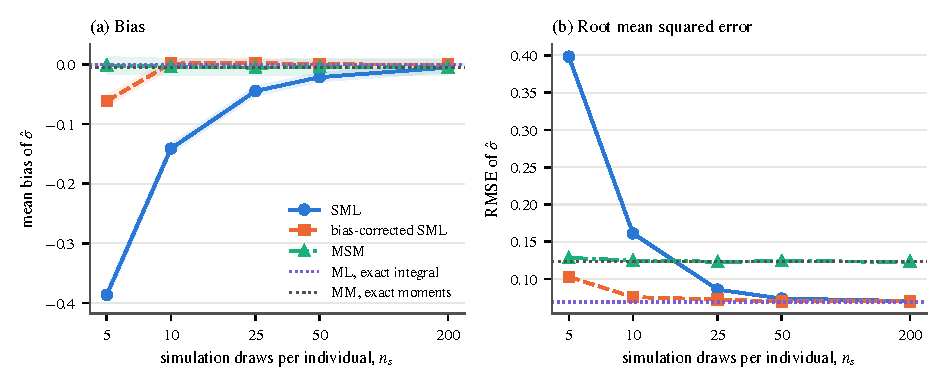
\includegraphics[width=\textwidth]{figures/appA/simest.pdf}
\caption{Simulation estimators of the standard deviation $\sigma$ of a random coefficient. Panel (a) shows the
mean bias of $\hat\sigma$ and panel (b) its root mean squared error, against the number of draws per individual.
The design is a panel binary logit with $N = 1{,}000$ individuals, $T = 5$ choices each, $x_{it} \sim N(0.5, 1)$,
$b_0 = -0.5$, $b_1 = 1$, $\sigma = 1$. SML uses \eqref{eq:A-sml}, bias-corrected SML adds
$\frac{\hat V_i}{2\tilde f_i^2}$, and MSM solves three simulated moment equations. The horizontal lines are maximum
likelihood and the exact-moment estimator computed with 40-point Gauss-Hermite quadrature. Shaded bands are
$\pm 1.96$ Monte Carlo standard errors. 300 replications, seed 20261022.}
\label{fig:A-simest}
\end{figure}

The results match the theory. With $n_s = 5$ draws, SML underestimates $\sigma = 1$ by 0.386 on average, and the
bias falls to 0.142, 0.045, 0.022 and 0.006 at 10, 25, 50 and 200 draws. From 25 draws on, $n_s$ times the bias is
roughly constant, as the $\frac{1}{n_s}$ rate predicts. The
bias pulls $\hat\sigma$ down because a smaller $\sigma$ makes the individual likelihood terms less variable across
draws, which raises $\E[\ln\tilde f_i]$ in part (i) of the proposition. The bias spills over to the mean coefficient
$b_1$, which is too small by 0.161 at five draws. The corrected estimator cuts the bias in $\hat\sigma$ to 0.062 at
five draws and to less than 0.003 from ten draws on. MSM is consistent at every fixed $n_s$, as \cref{prop:A-msm} predicts, and its Monte Carlo bias is small at every
$n_s$ in the table.
Its standard deviation at five draws is 0.129, against 0.123 with exact moments. The ratio of 1.04 is below the
bound $\sqrt{1 + \frac{1}{5}} = 1.10$ because the logit simulator is smooth. MSM's root mean squared error of about
0.12 exceeds that of maximum likelihood (0.069) at every $n_s$. Three just-identifying moments use the information
in the data less efficiently than the likelihood. SML overtakes MSM between 10 and 25 draws, and the corrected
version does so already at five.

\casehead{A worked case: Gentzkow (2007)}
\citet{Gentzkow2007} estimates a demand system for print and online newspapers in Washington, DC, from survey reports
of reading over the last day and the last five weekdays (\cref{sec:10-gentzkow}). The likelihood of a respondent's
report integrates a product of daily logit probabilities over a three-dimensional normal vector of random effects
(his eq.~6). He uses SML with 300 draws per consumer and the first-order bias correction of
\citet[p.~45]{GourierouxMonfort1996}. His footnote 32 derives the correction by the expansion in
\cref{prop:A-sml-bias}(i) (p.~732). The draws come from the importance density of \cref{lem:A-importance}. For each consumer he computes the
probability of the observed report once, at a preliminary estimate and with 200 draws. He then draws the random
effects from their distribution conditional on the report, by acceptance and rejection, and reweights
(p.~732, n.~31 and eqs.~13--14). Standard errors use the robust formula of \citet{McFaddenTrain2000}. Standard
errors of welfare statistics come from 100 draws from the estimated asymptotic distribution of the parameters
(p.~733), a method we discuss in \cref{sec:A-krinsky-robb}. He chose SML over MSM for the reasons given above. In
preliminary tests the two gave similar parameters, and MSM took 10 to 20 times longer to compute (p.~732). The
sample has 16,179 respondents (Table~5), large enough that the correction for $n_s = 300$ matters little, as in
\cref{fig:A-simest}. \Cref{sec:10-gentzkow-sml} gives the full estimator.

\subsection{Simulated nonlinear least squares}\label{sec:A-snlls}

\citet{LaffontOssardVuong1995} faced an integral inside a regression function. In a first-price or descending
auction with independent private values, the equilibrium bid function has no closed form for most value
distributions. The support of the winning bid also depends on the parameters. Maximum likelihood is then both
non-regular and computationally heavy, since the bid function must be inverted for every observation and every trial
parameter (p.~958, see \cref{prop:A-uniform-mle}). They proposed a least-squares estimator based on a simulated
conditional mean that is consistent for a fixed number of draws.

\casehead{The naive estimator and its limit}
Index auctions by $l = 1, \dots, n$ (their $L$), and let $b^w_l$ be the winning bid, with $b^w_l = p^o_l$ when the
object is unsold and $p^o_l$ the reserve price. Let $x_l$ collect the reserve price and the auction characteristics,
and let $m_l(\theta) = \E[b^w_l \mid x_l]$. Nonlinear least squares would minimize $\frac{1}{n}\sum_l(b^w_l -
m_l(\theta))^2$. Suppose $\bar X_l(\theta) = \frac{1}{n_s}\sum_{s=1}^{n_s}X_{sl}(\theta)$ is an unbiased simulator of
$m_l(\theta)$, with draws independent of $b^w_l$ given $x_l$. The naive estimator minimizes (their eq.~8)
\begin{equation}\label{eq:A-lov-naive}
  Q^{\text{naive}}_n(\theta) = \frac{1}{n}\sum_{l=1}^{n}\bigl(b^w_l - \bar X_l(\theta)\bigr)^2.
\end{equation}
To find its limit, write $b^w_l - \bar X_l(\theta) = (b^w_l - m_l(\theta_0)) + (m_l(\theta_0) - m_l(\theta)) +
(m_l(\theta) - \bar X_l(\theta))$. Given $x_l$, the first and third terms have mean zero and are independent of
each other, and the second is fixed. All cross products therefore have conditional mean zero, and
\begin{equation}\label{eq:A-lov-decomp}
  \E\bigl[(b^w_l - \bar X_l(\theta))^2 \mid x_l\bigr] = \sigma_0^2(x_l) + \bigl(m_l(\theta_0) - m_l(\theta)\bigr)^2
  + \frac{1}{n_s}\,\omega_l(\theta),
\end{equation}
where $\sigma_0^2(x_l) = \Var(b^w_l \mid x_l)$ and $\omega_l(\theta) = \Var(X_{sl}(\theta) \mid x_l)$. The first term
does not depend on $\theta$, and the second is minimized at $\theta_0$. The third term is the average simulator
variance, $A_L(\theta)$ in their eq.~(9). It depends on $\theta$, so the naive estimator converges to a value that
trades fit for a smaller simulator variance. It is inconsistent for fixed $n_s$ whenever the gradient of the
average simulator variance is nonzero at $\theta_0$, which is the generic case.

\casehead{The corrected estimator}
The sample variance of the draws, divided by $n_s$, is unbiased for $\frac{1}{n_s}\omega_l(\theta)$. Subtracting it
gives the simulated nonlinear least squares (SNLLS) objective (their eqs.~10--11):
\begin{equation}\label{eq:A-lov-snlls}
  Q^*_n(\theta) = \frac{1}{n}\sum_{l=1}^{n}\Bigl[\bigl(b^w_l - \bar X_l(\theta)\bigr)^2
  - \frac{1}{n_s(n_s - 1)}\sum_{s=1}^{n_s}\bigl(X_{sl}(\theta) - \bar X_l(\theta)\bigr)^2\Bigr].
\end{equation}
By \eqref{eq:A-lov-decomp}, each bracket has conditional mean $\sigma_0^2(x_l) + (m_l(\theta_0) - m_l(\theta))^2$, the
limit of exact nonlinear least squares. The estimator is consistent for any fixed $n_s$ as $n \to \infty$ (their
Proposition~1), and $Q^*_n(\hat\theta)$ consistently estimates the mean squared error of the model.

Its asymptotic variance shows the price of simulation (their Proposition~2). Let $\mu_l = \frac{\partial
m_l(\theta_0)}{\partial\theta}$, let $Y_{sl}(\theta) = \frac{\partial X_{sl}(\theta)}{\partial\theta}$, and let
$\omega_l$, $\Omega_l$ and $C_l$ be the conditional variances of $X_{sl}(\theta_0)$ and $Y_{sl}(\theta_0)$ and their
covariance. Then $\sqrt n(\hat\theta - \theta_0) \xrightarrow{d} N(0, \mathcal{H}^{-1}\mathcal{J}\mathcal{H}^{-1})$ with
$\mathcal{H} = \E[\mu_l\mu_l^\top]$ and
\begin{equation}\label{eq:A-lov-avar}
  \mathcal{J} = \E\Bigl[\sigma_0^2(x_l)\mu_l\mu_l^\top + \frac{1}{n_s}\bigl(\sigma_0^2(x_l)\Omega_l + \omega_l\mu_l\mu_l^\top\bigr)
  + \frac{1}{n_s(n_s - 1)}\bigl(\omega_l\Omega_l + C_lC_l^\top\bigr)\Bigr].
\end{equation}
The first term alone gives the variance of exact nonlinear least squares. The excess is of order $\frac{1}{n_s}$
and disappears as $n_s \to \infty$. Their Proposition~3 gives a heteroskedasticity-robust estimator of
$\mathcal{H}^{-1}\mathcal{J}\mathcal{H}^{-1}$ that is also consistent for fixed $n_s$.

\casehead{The simulator: revenue equivalence}
The construction of $X_{sl}$ uses auction theory. Let $N$ bidders (their $I$) have independent values from $F_l(\cdot;\theta)$
with density $f_l$, and let $v_{(N)}$ and $v_{(N-1)}$ be the highest and second-highest values. For a value $v \ge
p^o$, the first-price equilibrium bid equals the expected payment of the winner in a second-price auction (their
Lemma, eq.~12):
\begin{equation*}
  e(v) = \E\bigl[\max(v_{(N-1)}, p^o) \mid v_{(N)} = v\bigr].
\end{equation*}
The winning bid is $e(v_{(N)})$ when the object sells, and the convention $b^w = p^o$ covers the unsold case. Taking
expectations over $v_{(N)}$ with the law of iterated expectations gives (their eq.~14)
\begin{equation*}
  m_l(\theta) = \E\bigl[\max(v_{(N-1)l}, p^o_l)\bigr]
  = \int\!\!\cdots\!\!\int\max\bigl(u_{(N-1)}, p^o_l\bigr)\prod_{i=1}^{N}f_l(u_i;\theta)\,\dd u_1\cdots\dd u_N.
\end{equation*}
This is the revenue equivalence theorem at work: the expected winning bid equals the expected second-highest value,
truncated at the reserve price (\cref{ch:auction-theory}). The integrand needs no bid function. With importance
densities $g_l$ and draws $u^s_{1l}, \dots, u^s_{Nl}$ from $g_l$, the simulator is (their eq.~17)
\begin{equation*}
  X_{sl}(\theta) = \max\bigl(u^s_{(N-1)l}, p^o_l\bigr)\prod_{i=1}^{N}\frac{f_l(u^s_{il};\theta)}{g_l(u^s_{il})}.
\end{equation*}
The parameter appears only in the density ratio outside the maximum, so $Q^*_n$ is twice continuously
differentiable when $f_l$ is. Simulating with draws from $F_l(\cdot;\theta)$ would instead put $\theta$ inside the
maximum. With draws $F_l^{-1}(U^s_{il};\theta)$ from fixed uniforms $U^s_{il}$, the maximum is continuous in $\theta$ but
kinked where the reserve starts to bind. A frequency simulator built from indicators of simulated events would be a
step function of $\theta$. Neither would make $Q^*_n$ twice continuously differentiable.

\casehead{The application}
The data are 81 descending auctions of greenhouse eggplants in Marmande, France, in the summer of 1990, each selling
a single case (p.~967). Values are log-normal, with the mean of log values linear in six auction characteristics and
the standard deviation fixed at 0.05 from retail price dispersion (pp.~968--969). The estimates use 20 draws per
auction, and 30 draws gave analogous results (p.~969, n.~19). The number of bidders is treated as an unknown integer.
The criterion is minimized over $N$ from 11, the number of regular buyers, to 23, and the minimum is at $N = 18$
(p.~970). This suggests that one large buyer acts for about eight retailers. The fit gives an $R^2$ of 0.895 (p.~971).
\Cref{ch:auction-empirics} discusses the estimates.

\subsection{Indirect inference}\label{sec:A-indirect}

\emph{Indirect inference} \citep{GourierouxMonfortRenault1993,Smith1993} fits a simple auxiliary model to the real
data and to data simulated from the structural model. It chooses $\theta$ so that the two fits agree. Let
$\hat\beta$ be an auxiliary estimator, such as OLS coefficients or the parameters of a reduced-form logit, computed
on the data. For a trial $\theta$, simulate $H$ data sets of the same size from the structural model with fixed
draws, compute $\tilde\beta_h(\theta)$ on each, and average them into $\bar\beta(\theta)$. The estimator is
\begin{equation*}
  \hat\theta = \argmin_\theta\bigl(\hat\beta - \bar\beta(\theta)\bigr)^\top W\bigl(\hat\beta - \bar\beta(\theta)\bigr).
\end{equation*}
The probability limit of $\tilde\beta_h(\theta)$ is the \emph{binding function} $b(\theta)$, and identification
requires $b$ to be one to one near $\theta_0$. The auxiliary model need not be correctly specified. If
$\sqrt n(\hat\beta - b(\theta_0))$ has asymptotic variance $\Lambda$, the $H$ independent simulated estimates have
the same variance each, so the average has variance $\frac{\Lambda}{H}$. The estimator therefore behaves like a
minimum-distance estimator with variance inflated by the factor $(1 + \frac{1}{H})$, the analogue of
\cref{prop:A-msm}. MSM is the special case in which the auxiliary statistics are sample moments.

\subsection{Inference on functions of estimated parameters}\label{sec:A-krinsky-robb}

Many reported quantities are nonlinear functions $a(\theta)$ that are themselves computed by simulation: median
margins, welfare changes, predicted auction outcomes. The delta method of \cref{sec:A-delta} needs the derivative of
$a$, which may be costly or unstable. \citet{KrinskyRobb1986} proposed a simulation alternative.

\begin{remark}[Drawing from the estimated asymptotic distribution]\label{rem:A-krinsky-robb}
Given $\hat\theta$ and an estimate $\hat V$ of its variance:
\begin{enumerate}[label=(\arabic*)]
  \item Draw $\theta^{(1)}, \dots, \theta^{(R)}$ independently from $N(\hat\theta, \hat V)$.
  \item Compute $a(\theta^{(r)})$ for each draw, solving any equilibrium or simulation problem that $a$ requires.
  \item Report the standard deviation of the $a(\theta^{(r)})$, or their 2.5 and 97.5 percentiles as a 95 percent
  interval.
\end{enumerate}
\end{remark}

The method is common in the book's applications. \citet[Table~VIII, note]{Nevo2001} computes 95 percent intervals
for median margins from 1,500 draws (\cref{sec:08-nevo01}). \citet[p.~733]{Gentzkow2007} uses 100 draws for welfare
statistics. \citet[p.~248]{AtheyLevinSeira2011} call their version a parametric bootstrap. They resample from the
asymptotic distribution of the bid and entry parameters and recompute the expected auction outcomes for each draw.

The method rests on the same approximation as the delta method, the normality of $\hat\theta$. It retains the
nonlinearity of $a$, which helps when $a$ is far from linear over the likely range of $\theta$. It does not correct a
poor normal approximation for $\hat\theta$ itself, and it does not resample the data. \Cref{sec:A-boot-multistep}
compares it with bootstraps that re-estimate the model.

\section{Standard errors under dependence}\label{sec:A-se}

The variance formulas of \cref{sec:A-ols,sec:A-gmm} assume independent observations. Industrial organization data
rarely satisfy that assumption. Prices of the same product are observed in many cities, products in the same market
share demand shocks, and a state's prices are observed every year. This section derives the cost of ignoring such
dependence and the estimators that allow for it.

\subsection{One formula for all robust variances}\label{sec:A-se-meat}

Consider the linear model $y = X\beta + e$ with $n$ observations and $K$ regressors, and the OLS estimator
$\hat\beta = (X^\top X)^{-1}X^\top y$. Its sampling error is $\hat\beta - \beta = (X^\top X)^{-1}\sum_i x_ie_i$, so
conditional on $X$
\begin{equation}\label{eq:A-sandwich-general}
  \Var(\hat\beta \mid X) = (X^\top X)^{-1}\,\Omega_n\,(X^\top X)^{-1}, \qquad
  \Omega_n = \sum_{i=1}^{n}\sum_{j=1}^{n}x_ix_j^\top\E[e_ie_j \mid X].
\end{equation}
Every robust variance estimator replaces the ``meat'' $\Omega_n$ by
\begin{equation}\label{eq:A-meat-kernel}
  \hat\Omega_n = \sum_{i=1}^{n}\sum_{j=1}^{n}k_{ij}\,x_ix_j^\top\hat e_i\hat e_j,
\end{equation}
for weights $k_{ij} \in [0, 1]$ that state which pairs of observations may be correlated. The estimators differ only
in $k_{ij}$:
\begin{itemize}
  \item Heteroskedasticity-robust estimators (HC, \citealp{White1980}) set $k_{ij} = \indic\{i = j\}$.
  \item Cluster-robust estimators set $k_{ij} = \indic\{c(i) = c(j)\}$, with $c(i)$ the cluster of observation $i$.
  \item The Newey-West estimator for a time series sets $k_{ij} = \max\{0, 1 - \frac{|t_i - t_j|}{m+1}\}$ for a lag
  length $m$.
  \item Two-way clustering sets $k_{ij} = \indic\{g(i) = g(j) \text{ or } h(i) = h(j)\}$ for two grouping variables.
  \item Spatial HAC estimators \citep{Conley1999} let $k_{ij}$ decline in the economic distance between $i$ and $j$.
\end{itemize}
Plugging $\hat e_i\hat e_j$ for $e_ie_j$ is useless for a single pair, but the sum over many pairs averages out the
noise. Each estimator is consistent when the pairs it drops are uncorrelated and the pairs it keeps are few relative
to the sample. \Cref{sec:A-ols-asy} covered the HC case, including the finite-sample versions HC1 to HC3. HC estimators
suffice when observations are independent. The rest of this section treats the other cases.

\subsection{Clustered data}\label{sec:A-cluster}

Let the observations fall into $C$ clusters, $c = 1, \dots, C$, with $n_c$ observations in cluster $c$. Errors are
independent across clusters and may be correlated within. We first measure the cost of ignoring the correlation.

\begin{proposition}[Moulton factor]\label{prop:A-moulton}
Let $y_{ic} = \alpha + \beta x_{ic} + e_{ic}$ with $C$ clusters of equal size $\bar n$. Conditional on the
regressor, let the errors be homoskedastic with variance $\sigma^2$, uncorrelated across clusters and equicorrelated
within clusters with correlation $\rho_e$. Let $\tilde x_{ic} = x_{ic} - \bar x$ and define the intra-cluster
correlation of the regressor as
\begin{equation*}
  \rho_x = \frac{\sum_{c}\sum_{i \ne j}\tilde x_{ic}\tilde x_{jc}}{(\bar n - 1)\sum_c\sum_i\tilde x_{ic}^2}.
\end{equation*}
Then
\begin{equation}\label{eq:A-moulton}
  \Var(\hat\beta \mid x) = \frac{\sigma^2}{\sum_c\sum_i\tilde x_{ic}^2}\,\bigl[1 + (\bar n - 1)\rho_x\rho_e\bigr].
\end{equation}
The first factor is the conventional OLS variance. If the regressor is constant within clusters, $\rho_x = 1$ and the
factor is $1 + (\bar n - 1)\rho_e$.
\end{proposition}

\begin{proof}
By the Frisch-Waugh-Lovell theorem, $\hat\beta - \beta = \frac{\sum_c\sum_i\tilde x_{ic}e_{ic}}{\sum_c\sum_i\tilde
x_{ic}^2}$. Write $D = \sum_c\sum_i\tilde x_{ic}^2$. The numerator has variance
\begin{align*}
  \Var\Bigl(\sum_c\sum_i\tilde x_{ic}e_{ic}\Bigr)
  &= \sum_c\Bigl[\sum_i\tilde x_{ic}^2\sigma^2 + \sum_{i \ne j}\tilde x_{ic}\tilde x_{jc}\rho_e\sigma^2\Bigr] \\
  &= \sigma^2D + \rho_e\sigma^2(\bar n - 1)\rho_xD \\
  &= \sigma^2D\,\bigl[1 + (\bar n - 1)\rho_x\rho_e\bigr].
\end{align*}
The first line uses independence across clusters and the equicorrelation within. The second substitutes the
definition of $\rho_x$. Dividing by $D^2$ gives \eqref{eq:A-moulton}. If $x$ is constant within clusters, every
cross product $\tilde x_{ic}\tilde x_{jc}$ equals $\tilde x_{ic}^2$, so the numerator of $\rho_x$ is $(\bar n - 1)D$.
\end{proof}

The factor can be large even when $\rho_e$ is modest. With 20 observations per cluster and $\rho_x = \rho_e = 0.5$,
it equals $1 + 19 \times 0.25 = 5.75$, so the true standard error is $\sqrt{5.75} = 2.40$ times the conventional one.
A nominal 5 percent $t$-test that uses the conventional standard error then rejects a true null with probability
about $\Pr(|Z| > \frac{1.96}{2.40}) = 0.41$ in large samples. With unequal cluster sizes, \citet{Moulton1986} shows
that $\bar n - 1$ is replaced by $\frac{\Var(n_c)}{\bar n} + \bar n - 1$. \citet{Moulton1990} documents the problem
for regressions of individual outcomes on aggregate variables, where $\rho_x = 1$.

\casehead{The cluster-robust variance}
The cluster-robust estimator of \citet{LiangZeger1986} sets $k_{ij} = \indic\{c(i) = c(j)\}$ in
\eqref{eq:A-meat-kernel}. With $X_c$ and $\hat e_c$ the rows of cluster $c$, and the finite-sample factor used by
most software, it is
\begin{equation}\label{eq:A-cr1}
  \hat V_{\text{CR1}} = \frac{C}{C - 1}\,\frac{n - 1}{n - K}\,(X^\top X)^{-1}\Bigl(\sum_{c=1}^{C}X_c^\top\hat e_c\hat e_c^\top
  X_c\Bigr)(X^\top X)^{-1}.
\end{equation}
It allows any correlation and heteroskedasticity within clusters. Its consistency rests on the number of clusters.
When cluster sizes are bounded and $C \to \infty$, the terms $X_c^\top e_ce_c^\top X_c$ are independent across
clusters, and $\frac{1}{C}\sum_cX_c^\top e_ce_c^\top X_c$ converges to its mean by a law of large numbers.
Replacing $e_c$ by $\hat e_c$ changes the average by $o_p(1)$ because $\hat\beta$ is consistent. When each
observation is its own cluster, $C = n$ and $\frac{C}{C - 1}\frac{n - 1}{n - K} = \frac{n}{n - K}$, so CR1 reduces
to HC1. For 2SLS, replace $X$ by $\hat X = P_ZX$ in the bread and $x_i\hat e_i$ by $\hat x_i\hat e_i$ in the meat,
with residuals computed from $X$. For GMM, estimate the long-run covariance of the moments by
$\hat S = \frac{1}{n}\sum_c\hat g_c\hat g_c^\top$ with $\hat g_c = \sum_{i \in c}g(w_i;\hat\theta)$. When fixed
effects are nested within clusters, software differs on whether $K$ counts them. We count every regressor,
including the dummies, which gives slightly larger standard errors.

\casehead{The level of clustering}
The cluster should contain every pair of observations whose errors may be correlated, and clusters must be
numerous. \citet{BertrandDufloMullainathan2004} show the stakes for difference-in-differences regressions on
state-year panels.\footnote{We read NBER Working Paper 8841 (2002), the working-paper version of
\citet{BertrandDufloMullainathan2004}. Pages marked WP refer to it.} Placebo state laws, assigned at random, were
``significant'' at the 5 percent level in up to 45 percent of their simulations with conventional standard errors
(WP p.~3). Outcomes and treatment indicators are both serially correlated within states. Clustering by state, the
level at which treatment is assigned, restored approximately correct size with many states. The rejection rate was
6 percent in their panel of 51 states, and it rose to 8.5 percent with 10 states and 15 percent with 6 states (WP p.~18 and Table~9).
\citet{AbadieEtAl2023} add a design-based view. Clustering adjusts for
clustered sampling or clustered assignment of the regressor of interest. Correlated outcomes alone do not call for it
when assignment is at the individual level and the sample covers the population.

\casehead{Two-way clustering}
In a state-year panel, errors may be correlated within states over time and within years across states. Two-way
clustering \citep{CameronGelbachMiller2011} keeps every pair that shares a state or a year. The indicator of that
event satisfies the inclusion-exclusion identity
\begin{equation*}
  \indic\{g(i) = g(j) \text{ or } h(i) = h(j)\} = \indic\{g(i) = g(j)\} + \indic\{h(i) = h(j)\}
  - \indic\{g(i) = g(j),\ h(i) = h(j)\}.
\end{equation*}
Substituting into \eqref{eq:A-meat-kernel} gives $\hat V_{\text{2way}} = \hat V_g + \hat V_h - \hat V_{g \cap h}$:
cluster by the first dimension, cluster by the second, and subtract the estimate clustered by their intersection. In a
panel with one observation per state-year, the intersection estimator is the HC estimator. The difference can fail to
be positive semidefinite in small samples, and then negative eigenvalues are set to zero. Asymptotic justification
requires the number of clusters in both dimensions to grow, so inference should use the smaller of the two counts.

\casehead{Few clusters}
With few clusters, CR1 standard errors are too small and $t$-statistics are far from normal. Two corrections are
standard \citep{CameronMiller2015}. The first compares the $t$-statistic with the quantiles of the $t$ distribution
with $C - 1$ degrees of freedom. The second is the wild cluster bootstrap of \citet{CameronGelbachMiller2008}.

\begin{remark}[Wild cluster bootstrap-$t$]\label{rem:A-wild-cluster}
To test $H_0: \beta_k = \beta_k^0$ with CR1 standard errors:
\begin{enumerate}[label=(\arabic*)]
  \item Compute $t = \frac{\hat\beta_k - \beta_k^0}{\widehat{\mathrm{se}}_{\text{CR1}}(\hat\beta_k)}$ from the data.
  \item Estimate the model with the null imposed, and keep its coefficients $\tilde\beta$ and residuals $\tilde e_{ic}$.
  \item For $b = 1, \dots, B$, draw one weight $w_c^{(b)} \in \{-1, 1\}$ per cluster, each value with probability
  $\frac{1}{2}$ (Rademacher weights), and form $y^{(b)}_{ic} = x_{ic}^\top\tilde\beta + w_c^{(b)}\tilde e_{ic}$.
  \item Regress $y^{(b)}$ on $X$, and compute $t^{(b)} = \frac{\hat\beta^{(b)}_k -
  \beta_k^0}{\widehat{\mathrm{se}}_{\text{CR1}}(\hat\beta^{(b)}_k)}$ with the same formula as in step (1).
  \item Report the $p$-value $\frac{1}{B}\sum_{b=1}^{B}\indic\{|t^{(b)}| \ge |t|\}$. Count as ties the values of
  $|t^{(b)}|$ that differ from $|t|$ only by rounding error. If $2^C \le B$, use all $2^C$ weight vectors in place
  of random draws, and set $B = 2^C$.
\end{enumerate}
\end{remark}

Three features make the procedure work. Multiplying a whole cluster's residuals by one weight preserves any
correlation pattern within the cluster. Imposing the null makes the bootstrap data satisfy the hypothesis being
tested, which improves size. The statistic is studentized, which yields the asymptotic refinement of
\cref{sec:A-boot}.

When very few clusters are treated, the residuals of treated clusters carry the treatment effect estimate and the wild
bootstrap fails \citep{MacKinnonWebb2017}. Methods that use the control clusters to estimate the error
distribution are then needed \citep{ConleyTaber2011}.

\casehead{Discreteness with Rademacher weights}
With Rademacher weights there are only $2^C$ weight vectors, each with probability $2^{-C}$. The vectors $w$ and
$-w$ give bootstrap estimates $\hat\beta^{(b)}_k - \beta^0_k$ of opposite sign and residuals of opposite sign, so
they give the same $|t^{(b)}|$. Hence $|t^{(b)}|$ takes at most $2^{C-1}$ distinct values \citep{CameronMiller2015}.
The vector of ones reproduces the data, so it and its negative give $|t^{(b)}| = |t|$ exactly. The \emph{exact
conditional bootstrap $p$-value} is the probability of $|t^{(b)}| \ge |t|$ over all $2^C$ vectors, given the data.
It is at least $\frac{2}{2^C}$, which equals $\frac{1}{16} = 0.0625$ when $C = 5$. A 5 percent test with five clusters
therefore never rejects. The $p$-value of step (5) with random draws is a simulation estimate of the exact
$p$-value. It can fall below $\frac{2}{2^C}$ when few draws hit the two tying vectors, and enumeration removes this
noise. Rounding error can also make a computed $|t^{(b)}|$ fall just below $|t|$ for a tying vector, which is why
step (5) counts ties explicitly. Weight distributions with more support points make the $p$-value finer.
With fewer than ten clusters, \citet{CameronMiller2015} recommend the six-point weights of \citet{Webb2013}. These put probability
$\frac{1}{6}$ on each of $\pm\sqrt{\frac{1}{2}}$, $\pm 1$ and $\pm\sqrt{\frac{3}{2}}$, which have mean zero and
variance one.

\begin{figure}[htbp]
\centering
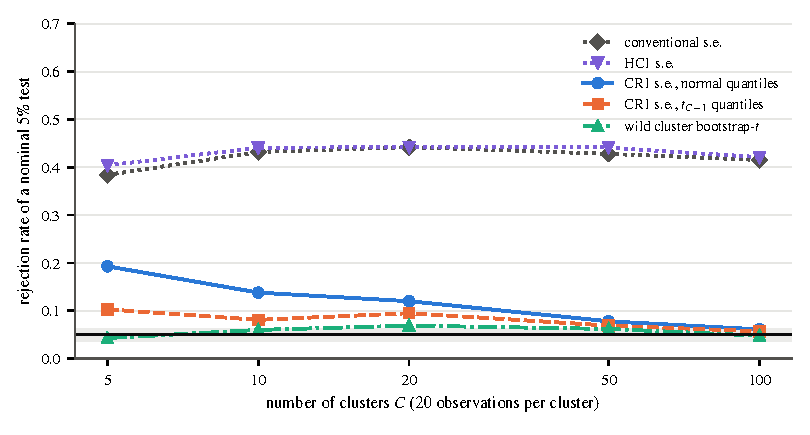
\includegraphics[width=0.86\textwidth]{figures/appA/cluster_mc.pdf}
\caption{Rejection rates of nominal 5 percent tests of a true null when errors and the regressor are both
correlated within clusters. In the design, $y_{ic} = e_{ic}$ is regressed on a constant and $x_{ic}$. Both $x_{ic}$
and $e_{ic}$ are sums of independent normal cluster and idiosyncratic components, with intra-cluster correlations
$\rho_x = \rho_e = 0.5$. There are 20 observations per cluster and 1,000 replications per $C$, with seed 20261022.
With $C = 5$ the Rademacher bootstrap enumerates all 32 weight vectors. The six-point bootstrap uses 399 random
weight vectors for every $C$, and the Rademacher bootstrap does so for $C \ge 10$. The gray band is the 95 percent Monte Carlo range around 0.05.}
\label{fig:A-cluster-mc}
\end{figure}

\Cref{fig:A-cluster-mc} reports a simulation with the parameters of the Moulton example. The conventional test
rejects the true null in 38 to 44 percent of replications for every number of clusters, close to the 41 percent
predicted above. HC1 standard errors do no better, because the problem is correlation, which HC1 ignores.
CR1 standard errors with normal quantiles reject 19 percent of the time with 5 clusters, 14 percent with 10 and 6
percent with 100. Using $t_{C-1}$ quantiles lowers the rejection rate to 10 percent with 5 clusters and 8 to 10
percent with 10 to 20 clusters. With Rademacher weights and at least 10 clusters, the wild cluster bootstrap rejects
between 4.8 and 6.9 percent of the time. With 5 clusters it never rejects, because its exact $p$-value is at least
0.0625 in every replication. A $p$-value simulated from 399 random draws would reject in 1.0 percent of the
replications with ties counted, and in 4.3 percent if rounding error drops the ties. The near-nominal second
figure is an artifact of the tie comparison. The six-point weights reject between 4.8 and 7.5 percent of the time
for every $C$, and 5.6 percent with 5 clusters. Each rate has a Monte Carlo standard error of about 0.007.

\subsection{Serial correlation and HAC estimators}\label{sec:A-hac}

In a time series $t = 1, \dots, T$, let $g_t$ be a mean-zero score or moment, for example $x_te_t$. Write
$\Gamma_j = \E[g_tg_{t-j}^\top]$ for its autocovariance at lag $j$, with $\Gamma_{-j} = \Gamma_j^\top$. Under
covariance stationarity,
\begin{equation*}
  \Var\Bigl(\frac{1}{\sqrt T}\sum_{t=1}^{T}g_t\Bigr) = \frac{1}{T}\sum_{t=1}^{T}\sum_{s=1}^{T}\Gamma_{t-s}
  = \sum_{j=-(T-1)}^{T-1}\Bigl(1 - \frac{|j|}{T}\Bigr)\Gamma_j \longrightarrow S = \sum_{j=-\infty}^{\infty}\Gamma_j,
\end{equation*}
where the middle step counts the $T - |j|$ pairs with $t - s = j$ and the limit holds when the autocovariances are
absolutely summable. The matrix $S$ is the \emph{long-run variance}. With $g_t = x_te_t$ and $n = T$, the meat
$\Omega_n$ of \eqref{eq:A-sandwich-general} is the variance of $\sum_tg_t$, which is approximately $TS$. An estimate
$\hat S$ therefore enters the OLS sandwich as $\hat\Omega_n = T\hat S$:
\begin{equation*}
  \widehat\Var(\hat\beta) = (X^\top X)^{-1}\,T\hat S\,(X^\top X)^{-1} = \frac{1}{T}\,\hat Q^{-1}\hat S\hat Q^{-1},
  \qquad \hat Q = \frac{X^\top X}{T}.
\end{equation*}
In the GMM formulas, $\hat S$ replaces $S$ directly.

\begin{example}[AR(1) regressor and error]\label{ex:A-ar1-factor}
Let $x_t$ and $e_t$ be independent stationary AR(1) processes with autocorrelations $\rho_x$ and $\rho_e$. Then
$\Gamma_j = \E[x_tx_{t-j}]\E[e_te_{t-j}] = \sigma_x^2\sigma_e^2(\rho_x\rho_e)^{|j|}$, and
\begin{equation*}
  S = \sigma_x^2\sigma_e^2\Bigl[1 + 2\sum_{j=1}^{\infty}(\rho_x\rho_e)^j\Bigr]
  = \sigma_x^2\sigma_e^2\,\frac{1 + \rho_x\rho_e}{1 - \rho_x\rho_e}.
\end{equation*}
The conventional variance uses only $\Gamma_0 = \sigma_x^2\sigma_e^2$, so it is too small by the factor
$\frac{1 + \rho_x\rho_e}{1 - \rho_x\rho_e}$. With $\rho_x = 0.85$ and $\rho_e = 0.64$, the factor is 3.4 and the
standard error ratio is 1.8. These are the within-state autocorrelations of the tax and of the residual in the
cigarette panel of \cref{sec:A-sumner-se}.
\end{example}

\casehead{The Newey-West estimator}
A natural estimator truncates the sum at lag $m$ and uses sample autocovariances
$\hat\Gamma_j = \frac{1}{T}\sum_{t=j+1}^{T}\hat g_t\hat g_{t-j}^\top$. The unweighted truncated sum can fail to be
positive semidefinite. \citet{NeweyWest1987} downweight the autocovariances linearly:
\begin{equation}\label{eq:A-newey-west}
  \hat S_{\text{NW}} = \hat\Gamma_0 + \sum_{j=1}^{m}\Bigl(1 - \frac{j}{m+1}\Bigr)\bigl(\hat\Gamma_j + \hat\Gamma_j^\top\bigr).
\end{equation}
The Bartlett weights $1 - \frac{j}{m+1}$ guarantee a positive semidefinite estimate. To see why, form the block sums
$\hat B_t = \sum_{k=0}^{m}\hat g_{t-k}$ and consider $\frac{1}{(m+1)T}\sum_t\hat B_t\hat B_t^\top$, an average of
outer products and hence positive semidefinite. Expanding the product, $\hat g_{t-k}\hat g_{t-l}^\top$ appears for
each pair $(k, l)$, and the number of pairs with $k - l = j$ is $m + 1 - |j|$. The weight on lag $j$ is therefore
$\frac{m + 1 - |j|}{m+1} = 1 - \frac{|j|}{m+1}$, which reproduces \eqref{eq:A-newey-west} up to terms at the ends
of the sample. Consistency requires $m \to \infty$ with $\frac{m}{T} \to 0$. A common rule of thumb is $m =
\lfloor 4(\frac{T}{100})^{\frac{2}{9}}\rfloor$. In \citet[p.~634]{NeweyWest1994} this formula is only a preliminary
lag in an automatic procedure for the Bartlett kernel. The procedure uses it to estimate a constant $\hat\gamma$ and then
sets $m = \lfloor\hat\gamma T^{\frac{1}{3}}\rfloor$ (p.~635).
\citet{GenesoveMullin1998} report Newey-West standard errors with four lags for their quarterly sugar demand and
pricing equations (\cref{sec:03-sugar}).

\casehead{Panels}
In a panel with many units and a short time dimension, clustering by unit allows arbitrary serial correlation
within units, and nothing more is needed if units are independent. When units share common shocks that time
effects do not remove, \citet{DriscollKraay1998} average the scores across units within each period and apply
\eqref{eq:A-newey-west} to the resulting time series. Their estimator allows any cross-sectional dependence, but it
requires a long panel and allows only serial correlation that dies out within $m$ periods. \citet{Conley1999}
extends the HAC idea to dependence that declines with spatial or economic distance.

\subsection{Dependence structures in IO data}\label{sec:A-io-dependence}

The book's applications show four recurring structures. The first is the same product observed in many markets in
the same period, whose prices respond to common cost and demand shocks.
\citet[WP p.~25]{AshenfelterHosken2010} observe the prices of the same products in many geographic markets each
period,\footnote{We read NBER Working Paper 13859 (2008) of \citet{AshenfelterHosken2010} and NBER Working Paper
17476 (2011) of \citet{AshenfelterHoskenWeinberg2013}. Pages marked WP refer to them.} and therefore cluster on the time period, citing \citet{Moulton1987}. Their reference list contains only
\citet{Moulton1990} (WP p.~39), which makes the same point about aggregate regressors. The second is the same product or
unit observed repeatedly over time. \citet[WP p.~14]{AshenfelterHoskenWeinberg2013} cluster by SKU in their
appliance price regressions. \citet[pp.~862--863]{BerryLevinsohnPakes1995} treat the sum of the moments of a car model over
all its years as one observation, which allows any correlation across years for a given model. The third is common
shocks to all products in a market. \citet[WP p.~17]{BerryCarnallSpiller1996} assume independence across airline
markets and a factor structure that correlates demand and cost errors within a market (\cref{sec:09-bcs-estimation}).
They also note that the average product has fewer than 10 sampled passengers, and they leave the correction of
standard errors for this sampling error to future research (WP p.~17). The fourth
is serial correlation that a structural model must represent explicitly. \citet{Ellison1994} models an AR(1) demand
error inside his Markov-switching likelihood, and doing so changes the point estimates as well as the standard
errors (\cref{ch:collusion-evidence}). \Cref{tab:A-se-practice} collects the inference methods used in the book.

\begin{table}[htbp]
\centering
\begin{threeparttable}
\caption{Inference under dependence in the book's applications}
\label{tab:A-se-practice}
\footnotesize
\begin{tabularx}{\textwidth}{@{}>{\raggedright\arraybackslash}p{2.7cm}>{\raggedright\arraybackslash}X>{\raggedright\arraybackslash}X>{\raggedright\arraybackslash}p{2.6cm}@{}}
\toprule
Application & Data structure & Inference used & Source \\
\midrule
\citet{Sumner1981}, re-estimated & State-year panel, 48 units, 25 years & Clusters by state, by year and both, Driscoll-Kraay, wild cluster bootstrap & \Cref{tab:A-sumner} \\
\addlinespace
\citet{GenesoveMullin1998} & Quarterly time series, 1890--1914 & Newey-West, 4 lags, with the pricing equation corrected for estimated demand & \Cref{sec:03-sugar} \\
\addlinespace
\citet{AshenfelterHosken2010} & Product by city by period & Clusters on the time period & WP p.~25 \\
\addlinespace
\citet{AshenfelterHoskenWeinberg2013} & SKU by month & Clusters by SKU & WP p.~14 \\
\addlinespace
\citet{BerryLevinsohnPakes1995} & Car model by year & Moments summed over a model's years, simulation variance added & pp.~862--863 and \cref{sec:08-asymptotics} \\
\addlinespace
\citet{BerryCarnallSpiller1996} & Products in airline markets & Independence across markets and a factor structure within them, share sampling error not corrected & WP p.~17 and \cref{sec:09-bcs-estimation} \\
\addlinespace
\citet{MillerWeinberg2017} & Brand-size product by region by period & Clusters by region, two-step correction for estimated demand & pp.~1775, 1780 and \cref{ch:mergers} \\
\addlinespace
\citet{ChaudhuriGoldbergJia2006} & Product by region by month & Bootstrap over months, 300 replications, all products and regions kept & WP p.~21 \\
\addlinespace
\citet{Nevo2001} & Brand by city by quarter & 1,500 draws from the asymptotic distribution for median margins & Table~VIII \\
\addlinespace
\citet{Asker2010} & Auctions & Bootstrap over auctions, 5,000 iterations, 90 percent intervals & Tables~7--10 \\
\addlinespace
\citet{Gentzkow2007} & Survey respondents & Robust SML standard errors, 100 parameter draws for welfare & p.~733 \\
\addlinespace
\citet{AtheyLevinSeira2011} & Timber sales & Matching standard errors of \citet{AbadieImbens2006}, parametric bootstrap & pp.~230, 248 \\
\bottomrule
\end{tabularx}
\begin{tablenotes}\footnotesize
\item Notes: WP page numbers refer to working-paper versions of the papers.
\end{tablenotes}
\end{threeparttable}
\end{table}

\subsection{Worked application: Sumner's regression revisited}\label{sec:A-sumner-se}

\citet{Sumner1981} tests for competition in cigarettes by regressing the retail price per pack on the excise tax in a
state-year panel (\cref{sec:A-panel,sec:03-sumner-design}). His most complete specification is the two-way fixed effects
regression \eqref{eq:A-sumner} of \cref{sec:A-panel},
\begin{equation*}
  p_{sy} = \mu_s + \tau_y + \rho\,t_{sy} + e_{sy},
\end{equation*}
with state effects $\mu_s$, year effects $\tau_y$ and pass-through $\rho$. Competition with flat marginal cost
implies $\rho = 1$. Sumner reports $\hat\rho = 1.074$ with a conventional standard error of 0.013 (Table~1), so the
$t$-statistic for $\rho = 1$ is 5.7. Both the price and the tax are persistent within states, so the
conventional standard error is suspect.

We re-estimate the regression on a panel reconstructed from \emph{The Tax Burden on Tobacco} (1983, Table~13) and
the CPI-U of the Bureau of Labor Statistics. It covers 47 states and the District of Columbia from 1954 to 1978,
1,200 state-years, the same coverage as Sumner's. Prices and taxes are nominal cents per pack, and the tax is the
state tax plus the federal tax of 8 cents. The computations are in \texttt{figures/appA/src/sumner\_inference.py}.
\Cref{tab:A-sumner} reports three specifications and six variance estimators.

\begin{table}[htbp]
\centering
\begin{threeparttable}
\caption{Cigarette tax pass-through: standard errors and tests of $\rho = 1$ under different dependence assumptions}
\label{tab:A-sumner}
\small
\setlength{\tabcolsep}{3.6pt}
\begin{tabular}{@{}lccccccccc@{}}
\toprule
& Sumner & \multicolumn{8}{c}{Re-estimation} \\
\cmidrule(lr){2-2}\cmidrule(l){3-10}
Specification & (1981) & $\hat\rho$ & Conv. & HC1 & State & Year & Two-way & DK & Wild \\
\midrule
(1) State, year effects, OLS & \makecell{1.074\\(0.013)} & 1.075 & 0.013 & 0.015 & 0.034 & 0.013 & 0.033 & 0.016 & \\
\quad $p$-value for $\rho = 1$ & & & $<$0.001 & $<$0.001 & 0.033 & $<$0.001 & 0.034 & $<$0.001 & 0.044 \\
\addlinespace
(2) CPI, OLS & \makecell{1.029\\(0.011)} & 1.029 & 0.011 & 0.013 & 0.030 & 0.023 & 0.035 & 0.027 & \\
\quad $p$-value for $\rho = 1$ & & & 0.007 & 0.030 & 0.340 & 0.207 & 0.416 & 0.299 & 0.358 \\
\addlinespace
(3) CPI, random effects & \makecell{1.069\\(0.013)} & 1.069 & 0.013 & 0.015 & 0.033 & 0.015 & 0.033 & 0.020 & \\
\quad $p$-value for $\rho = 1$ & & & $<$0.001 & $<$0.001 & 0.042 & $<$0.001 & 0.046 & 0.002 & \\
\bottomrule
\end{tabular}
\begin{tablenotes}\footnotesize
\item Notes: The dependent variable is the retail price in cents per pack and the regressor of interest the combined
state and federal tax in cents per pack, 1,200 state-years. The first column reproduces Sumner's Table~1 (standard
errors in parentheses). The other columns report our estimate of $\rho$ and its standard error under six
estimators. Conv.: conventional OLS or GLS. HC1: heteroskedasticity-robust. State and Year: CR1 clustered by state
(48 clusters) or by year (25). Two-way: clustered by state and year \citep{CameronGelbachMiller2011}. DK:
\citet{DriscollKraay1998} with Bartlett weights and 2 lags. $p$-values use normal quantiles for Conv.\ and HC1,
$t_{47}$ for State, $t_{24}$ for Year, Two-way and DK. Wild: wild cluster bootstrap-$t$ by state with the null
imposed, Rademacher weights and 9,999 draws. Row (2) replaces the year effects by the national CPI and drops the
state effects. Row (3) has the regressors of row (2) and is two-way random-effects GLS \citep{FullerBattese1974}, and
its robust variants apply the formulas to the GLS-transformed regression. $K$ counts all dummies in row (1).
\end{tablenotes}
\end{threeparttable}
\end{table}

\casehead{Row (1)}
The re-estimation reproduces Sumner's estimate and conventional standard error. The HC1 standard error is 15
percent larger. Clustering by state raises the standard error to 0.034, 2.6 times the conventional value. The
within-state first-order autocorrelation of the residuals is 0.64 and that of the within-transformed tax is 0.85.
\Cref{ex:A-ar1-factor} predicts a standard error ratio of about 1.8 for these values, and the ratio of the clustered to
the HC1 standard error is 2.2. Clustering by year leaves the standard error at 0.013. The year effects absorb the
common national shocks, so the residuals of different states in the same year are nearly uncorrelated. The two-way
estimate, 0.033, is close to the state-clustered one for the same reason. The Driscoll-Kraay estimate, 0.016, allows
any correlation across states but only two lags of serial correlation, and it misses the persistence that clustering
by state captures. The rejection of $\rho = 1$ survives every estimator that allows correlation within states, with
$p$-values from 0.033 to 0.044, but its margin is far thinner than a $t$-statistic of 5.7 suggests. The wild cluster
bootstrap $p$-value of 0.044 has a Monte Carlo standard error of 0.002.

\casehead{Row (2)}
Without state effects, persistent differences in state price levels enter the error, and they are correlated over
time within a state. The conventional standard error of 0.011 gives $p = 0.007$. Clustering by state, by year or by both, the
Driscoll-Kraay estimator and the wild cluster bootstrap all give $p$ above 0.2. The apparent rejection of competition in this specification is an
artifact of the conventional standard error.

\casehead{Row (3)}
The random-effects GLS estimate reproduces Sumner's 1.069. Its conventional standard error assumes that a constant
state effect captures all within-state correlation. The residuals of the transformed regression remain serially
correlated, and the state-clustered standard error is 0.033, with $p = 0.042$. Random effects therefore do not
substitute for clustering when the error has more persistence than a permanent effect.

The lesson is general. In a panel with persistent regressors and errors, the conventional and heteroskedasticity-robust
standard errors can overstate precision by a factor of two or more. The clustering level should follow the
dependence that the fixed effects leave in the error. Here the fixed effects leave serial correlation within
states, while the correlation across states within a year is negligible.

\section{The delta method and the bootstrap}\label{sec:A-delta-boot}

Empirical work rarely stops at the estimated parameters. A pass-through coefficient is turned into an elasticity,
demand parameters into markups, and a demand system into the welfare effect of a counterfactual. This section
develops the two general tools for the uncertainty of such quantities, the delta method and the bootstrap, and
shows when each fails.

\subsection{The delta method}\label{sec:A-delta}

\begin{theorem}[Delta method]\label{thm:A-delta}
Suppose $\sqrt n(\hat\theta - \theta_0) \xrightarrow{d} N(0, V)$ for $\theta_0 \in \R^K$. Let $a: \R^K \to \R^q$ be
continuously differentiable in a neighborhood of $\theta_0$, with Jacobian $A(\theta) = \frac{\partial
a(\theta)}{\partial\theta^\top}$ ($q \times K$) and $A = A(\theta_0)$. Then
\begin{equation*}
  \sqrt n\bigl(a(\hat\theta) - a(\theta_0)\bigr) \xrightarrow{d} N(0, AVA^\top).
\end{equation*}
If $\hat V \xrightarrow{p} V$, then $A(\hat\theta)\hat VA(\hat\theta)^\top \xrightarrow{p} AVA^\top$.
\end{theorem}

\begin{proof}
Since $\sqrt n(\hat\theta - \theta_0)$ converges in distribution, $\hat\theta - \theta_0 = O_p(n^{-\frac{1}{2}})$ and
$\hat\theta \xrightarrow{p} \theta_0$. For each component $a_k$, the mean value theorem gives a point $\bar\theta_k$
on the segment between $\hat\theta$ and $\theta_0$ with
\begin{equation*}
  a_k(\hat\theta) - a_k(\theta_0) = \frac{\partial a_k(\bar\theta_k)}{\partial\theta^\top}(\hat\theta - \theta_0).
\end{equation*}
Stack these rows into a matrix $\bar A$. Each $\bar\theta_k \xrightarrow{p} \theta_0$, so $\bar A \xrightarrow{p} A$
by continuity of the derivatives. Then
\begin{equation*}
  \sqrt n\bigl(a(\hat\theta) - a(\theta_0)\bigr) = \bar A\,\sqrt n(\hat\theta - \theta_0),
\end{equation*}
and Slutsky's theorem gives convergence to $A\,N(0, V) = N(0, AVA^\top)$. The second claim follows from the
continuous mapping theorem.
\end{proof}

In practice the delta-method standard error of a scalar $a(\hat\theta)$ is $\sqrt{\nabla a(\hat\theta)^\top\hat
V_n\nabla a(\hat\theta)}$, where $\hat V_n = \frac{\hat V}{n}$ is the estimated variance of $\hat\theta$. We now work
through the cases that recur in the book.

\begin{example}[Elasticity implied by pass-through]\label{ex:A-delta-passthrough}
Under monopoly or constant conduct with constant-elasticity demand and flat marginal cost, pass-through is $\rho =
\frac{\varepsilon}{\varepsilon - 1}$, where $\varepsilon$ is the elasticity the firms behave as if they face
(\cref{sec:03-sumner-design}). Inverting gives $\varepsilon = a(\rho) = \frac{\rho}{\rho - 1}$ for $\rho > 1$. The
derivative is
\begin{equation*}
  a'(\rho) = \frac{(\rho - 1) - \rho}{(\rho - 1)^2} = -\frac{1}{(\rho - 1)^2},
  \qquad \mathrm{se}(\hat\varepsilon) = \frac{\mathrm{se}(\hat\rho)}{(\hat\rho - 1)^2}.
\end{equation*}
Sumner's estimate $\hat\rho = 1.074$ with standard error 0.013 gives $\hat\varepsilon = \frac{1.074}{0.074} = 14.5$ and
a delta-method standard error of $\frac{0.013}{0.074^2} = 2.37$.\footnote{Sumner's printed implied elasticities equal
$\frac{1}{1 - \hat\rho}$, for example $-13.5$ for the first row. They are one unit smaller in magnitude than
$\frac{\hat\rho}{\hat\rho - 1}$, because they treat $\hat\rho - 1$ as the markup over cost instead of using the Lerner
condition (\cref{sec:03-sumner-design}).} Our re-estimate $\hat\rho = 1.0746$ gives $\hat\varepsilon = 14.4$, with a
standard error of 2.38 based on the conventional standard error and 6.11 based on the state-clustered one. The
standard error of $\hat\varepsilon$ is about 180 times that of $\hat\rho$, because the derivative is the inverse
square of $\hat\rho - 1 = 0.075$.
\end{example}

\begin{example}[Marginal cost from an inverse-elasticity rule]\label{ex:A-delta-cost}
With an observed price $p$ and an estimated elasticity, the Lerner rule $\frac{p - c}{p} = \frac{1}{\varepsilon}$
gives $\hat c = p(1 - \frac{1}{\hat\varepsilon})$ (\cref{prop:01-infer-cost}). The derivative
$\frac{\dd c}{\dd\varepsilon} = \frac{p}{\varepsilon^2}$ yields $\mathrm{se}(\hat c) = \frac{p}{\hat\varepsilon^2}
\mathrm{se}(\hat\varepsilon)$. Chaining with \cref{ex:A-delta-passthrough}, $c = p(1 - \frac{\rho - 1}{\rho}) =
\frac{p}{\rho}$, so $\mathrm{se}(\hat c) = \frac{p}{\hat\rho^2}\mathrm{se}(\hat\rho)$. The cost implied by
pass-through is precise even when the elasticity is not, because a markup of a few percent is small whatever its
exact value.
\end{example}

\begin{example}[Willingness to pay as a ratio]\label{ex:A-delta-ratio}
In a demand model with utility $x\beta - \alpha p$, the willingness to pay for characteristic $k$ is $r =
\frac{\beta_k}{\alpha}$. The gradient with respect to $(\beta_k, \alpha)$ is $(\frac{1}{\alpha}, -\frac{\beta_k}
{\alpha^2})$, so
\begin{equation*}
  \widehat{\Var}(\hat r) = \frac{1}{\hat\alpha^2}\Bigl[\hat V_{kk} - 2\hat r\hat V_{k\alpha} + \hat r^2\hat V_{\alpha\alpha}\Bigr],
\end{equation*}
with $\hat V$ the estimated covariance of $(\hat\beta_k, \hat\alpha)$. When $\hat\alpha$ is imprecise, the
distribution of the ratio is far from normal. \citet{Fieller1954} proposed an exact alternative under normality.
The statistic $\hat\beta_k - r\hat\alpha$ has mean zero at the true ratio and variance $V_{kk} - 2rV_{k\alpha} +
r^2V_{\alpha\alpha}$. The Fieller set collects the values $r$ that a test does not reject:
\begin{equation*}
  \bigl\{r : (\hat\beta_k - r\hat\alpha)^2 \le z^2\bigl(\hat V_{kk} - 2r\hat V_{k\alpha} + r^2\hat V_{\alpha\alpha}\bigr)\bigr\},
\end{equation*}
with $z$ the normal quantile. The inequality is quadratic in $r$, with leading coefficient $\hat\alpha^2 - z^2\hat
V_{\alpha\alpha}$. The set is a bounded interval if and only if this coefficient is positive, that is, if $\hat\alpha$
is significantly different from zero. Otherwise it is the whole line or the union of two half-lines, which correctly
signals that the data cannot bound the ratio.
\end{example}

\begin{example}[Elasticities and markups from demand parameters]\label{ex:A-delta-logit}
In the logit model, the own-price elasticity is $\varepsilon_{jj} = -\alpha p_j(1 - s_j)$ and the single-product markup is
$p_j - c_j = \frac{1}{\alpha(1 - s_j)}$ (\cref{ch:logit}). Both depend on the estimates only through $\hat\alpha$,
with derivatives $-p_j(1 - s_j)$ and $-\frac{1}{\alpha^2(1 - s_j)}$. The relative standard error of the markup
therefore equals that of $\hat\alpha$. In the AIDS model elasticities are functions of many parameters, and the
full gradient and covariance matrix are needed (\cref{ch:aids}).
\end{example}

\begin{example}[Log points and percentages]\label{ex:A-delta-log}
A coefficient $\beta$ on the log scale implies a proportional effect $a(\beta) = e^\beta - 1$, with
$\mathrm{se}(\hat a) = e^{\hat\beta}\mathrm{se}(\hat\beta)$. \citet{Dafny2009} estimates by instrumental variables
that a rival merger raises hospital price growth by 0.376 log points, with standard error 0.132 (WP Table~4, see
\cref{sec:A-ivmodel}). The implied increase is $e^{0.376} - 1 = 46$ percent, with delta-method standard error
$e^{0.376}\times 0.132 = 0.19$. The symmetric 95 percent interval is $[8, 83]$ percent. Mapping the endpoints of the
interval for $\beta$ through $e^\beta - 1$ gives $[12, 89]$ percent, which respects the asymmetry of the
transformation.
\end{example}

\casehead{When the delta method fails}
Three situations break the linear approximation. First, if $A = 0$ the first-order term vanishes. For scalar
$\theta$ with $a'(\theta_0) = 0$ and $a''(\theta_0) \ne 0$, a second-order expansion gives
$n(a(\hat\theta) - a(\theta_0)) \xrightarrow{d} \frac{1}{2}a''(\theta_0)V\chi^2_1$. For example, $n\hat\theta^2$
converges to $V\chi^2_1$ when $\theta_0 = 0$. Second, if $a$ is not differentiable at $\theta_0$, as with $|\theta|$,
$\max\{\theta_1, \theta_2\}$ at $\theta_1 = \theta_2$, or bounds defined by extrema, the limit is not normal.
Third, if $a$ is differentiable but very nonlinear over the region where $\hat\theta$ is likely to fall, the normal
approximation is poor in any finite sample. A denominator close to zero is the typical case.

\Cref{ex:A-delta-passthrough} is of the third kind. With the state-clustered standard error, the 95 percent
delta-method interval for the elasticity is $14.4 \pm 2.012 \times 6.11 = [2.1, 26.7]$, using $t_{47}$ quantiles. The
lower end corresponds to $\rho = \frac{2.1}{1.1} = 1.9$, a value far outside the confidence interval for $\rho$,
which is $[1.006, 1.143]$. A better interval maps the endpoints. Because $a(\rho) = \frac{\rho}{\rho - 1}$ is
strictly decreasing on $(1, \infty)$,
\begin{equation*}
  \Pr\bigl(a(\rho_0) \in [a(\rho_U), a(\rho_L)]\bigr) = \Pr\bigl(\rho_0 \in [\rho_L, \rho_U]\bigr)
\end{equation*}
whenever $\rho_L > 1$. The mapped interval inherits the exact coverage of the interval for $\rho$. Here it is
$[a(\rho_U), a(\rho_L)] = [\frac{1.1430}{0.1430}, \frac{1.006177}{0.006177}] = [8.0, 162.9]$, strongly asymmetric. We
show $\rho_L$ with more digits because the map is very steep near one. With the conventional standard error
the two intervals are $[9.7, 19.1]$ and $[10.9, 21.5]$, much closer, because $\hat\rho$ is then many standard errors
from one. If the interval for $\rho$ contained one, the set of elasticities consistent with the data would be
unbounded, and no symmetric interval could represent it. \Cref{fig:A-delta-boot} shows these intervals together
with a bootstrap distribution.

\subsection{The bootstrap: principle and theory}\label{sec:A-boot}

The bootstrap of \citet{Efron1979} estimates the sampling distribution of a statistic by recomputing it on samples
drawn from an estimate of the population. Let the data $w_1, \dots, w_n$ be independent draws from $F$, and let
$T_n = \sqrt n(\hat\theta - \theta_0)$ have distribution $G_n(\cdot, F)$. The \emph{plug-in principle} replaces the
unknown $F$ by the empirical distribution $\hat F_n$, which puts mass $\frac{1}{n}$ on each observation. The
bootstrap estimate of $G_n(\cdot, F)$ is $G_n(\cdot, \hat F_n)$, the distribution of $\sqrt n(\hat\theta^* -
\hat\theta)$ when $\hat\theta^*$ is computed from a sample of size $n$ drawn from $\hat F_n$. That distribution is
computed by simulation.

\begin{remark}[Nonparametric bootstrap]\label{rem:A-pairs-boot}
For $b = 1, \dots, B$:
\begin{enumerate}[label=(\arabic*)]
  \item Draw $n$ observations from $\{w_1, \dots, w_n\}$ with replacement.
  \item Compute the estimator on this sample, $\hat\theta^*_b$, with exactly the procedure used on the data.
\end{enumerate}
The bootstrap standard error is the standard deviation of $\hat\theta^*_1, \dots, \hat\theta^*_B$. In regression,
drawing whole observations $(y_i, x_i)$ is the \emph{pairs bootstrap}, which is robust to heteroskedasticity.
\end{remark}

\begin{proposition}[Bootstrap consistency for the mean]\label{prop:A-boot-mean}
Let $X_1, \dots, X_n$ be i.i.d.\ with variance $\sigma^2 > 0$ and $\E|X|^3 < \infty$. Let $\bar X^*$ be the mean of a
bootstrap sample. Then
\begin{equation*}
  \sup_x\Bigl|\Pr^*\bigl(\sqrt n(\bar X^* - \bar X) \le x\bigr) - \Pr\bigl(\sqrt n(\bar X - \mu) \le x\bigr)\Bigr|
  \xrightarrow{a.s.} 0,
\end{equation*}
where $\Pr^*$ is the probability over bootstrap draws given the data.
\end{proposition}

\begin{proof}
Given the data, $\bar X^*$ is the mean of $n$ independent draws from $\hat F_n$, which has mean $\bar X$, variance
$\hat\sigma^2 = \frac{1}{n}\sum_i(X_i - \bar X)^2$ and third absolute central moment $\hat\kappa_3 =
\frac{1}{n}\sum_i|X_i - \bar X|^3$. The Berry-Esseen inequality bounds the distance between the conditional
distribution of $\sqrt n(\bar X^* - \bar X)$ and $N(0, \hat\sigma^2)$:
\begin{equation*}
  \sup_x\Bigl|\Pr^*\bigl(\sqrt n(\bar X^* - \bar X) \le x\bigr) - \Phi\Bigl(\frac{x}{\hat\sigma}\Bigr)\Bigr|
  \le \frac{C_0\,\hat\kappa_3}{\hat\sigma^3\sqrt n},
\end{equation*}
for a universal constant $C_0$. By the strong law of large numbers, $\hat\sigma^2 \to \sigma^2$ and $\hat\kappa_3$
converges to a finite limit almost surely, so the bound tends to zero. The same inequality applied to the original
sample bounds the distance between the distribution of $\sqrt n(\bar X - \mu)$ and $\Phi(\frac{x}{\sigma})$ by a
term of order $n^{-\frac{1}{2}}$. Finally, $\sup_x|\Phi(\frac{x}{\hat\sigma}) - \Phi(\frac{x}{\sigma})| \to 0$ because
$\hat\sigma \to \sigma$. The triangle inequality combines the three bounds.
\end{proof}

The result extends to smooth functions of means, which include OLS, IV and GMM estimators, and to many other
statistics \citep{BickelFreedman1981,Hall1992}. The common structure is that $\hat\theta$ is asymptotically a smooth
function of averages, so the bootstrap reproduces the first-order normal approximation. \Cref{sec:A-boot-fail}
shows what happens without that structure.

\casehead{Confidence intervals}
Let $q^*_\alpha$ be the $\alpha$ quantile of the bootstrap estimates $\hat\theta^*_b$. Four intervals with nominal
coverage $1 - \alpha$ are standard.
\begin{enumerate}[label=(\roman*)]
  \item The \emph{percentile} interval is $[q^*_{\frac{\alpha}{2}}, q^*_{1-\frac{\alpha}{2}}]$.
  \item The \emph{basic} interval uses the bootstrap distribution of $\hat\theta^* - \hat\theta$ as an estimate of
  that of $\hat\theta - \theta_0$. From $\Pr(q^*_{\frac{\alpha}{2}} - \hat\theta \le \hat\theta - \theta_0 \le
  q^*_{1-\frac{\alpha}{2}} - \hat\theta) \approx 1 - \alpha$, solving for $\theta_0$ gives
  $[2\hat\theta - q^*_{1-\frac{\alpha}{2}},\ 2\hat\theta - q^*_{\frac{\alpha}{2}}]$.
  \item The \emph{percentile-$t$} interval bootstraps the studentized statistic $t^*_b = \frac{\hat\theta^*_b -
  \hat\theta}{\mathrm{se}^*_b}$, with $\mathrm{se}^*_b$ computed on bootstrap sample $b$ by the same formula as on the
  data. With $t^*_\alpha$ its quantiles, the interval is $[\hat\theta - t^*_{1-\frac{\alpha}{2}}\mathrm{se},\
  \hat\theta - t^*_{\frac{\alpha}{2}}\mathrm{se}]$.
  \item The \emph{bias-corrected and accelerated} (BCa) interval is $[q^*_{\tilde\alpha_1}, q^*_{\tilde\alpha_2}]$. Its
  adjusted levels are $\tilde\alpha_j = \Phi\bigl(z_0 + \frac{z_0 + z_{\alpha_j}}{1 - \hat a(z_0 + z_{\alpha_j})}\bigr)$
  for the nominal levels $\alpha_1 = \frac{\alpha}{2}$ and $\alpha_2 = 1 - \frac{\alpha}{2}$, with $z_{\alpha_j} =
  \Phi^{-1}(\alpha_j)$. The bias correction is $z_0 = \Phi^{-1}(\frac{1}{B}\sum_b\indic\{\hat\theta^*_b < \hat\theta\})$, and the
  acceleration $\hat a = \frac{\sum_i(\bar\theta_{(\cdot)} - \hat\theta_{(i)})^3}{6[\sum_i(\bar\theta_{(\cdot)} -
  \hat\theta_{(i)})^2]^{\frac{3}{2}}}$ comes from the leave-one-out estimates $\hat\theta_{(i)}$ and their mean
  $\bar\theta_{(\cdot)}$.
\end{enumerate}
The percentile and BCa intervals are \emph{transformation respecting}. If $a$ is monotone, the interval for
$a(\theta)$ is the image of the interval for $\theta$. The basic and percentile-$t$ intervals are not.

\casehead{Asymptotic refinement}
Under regularity conditions the distribution of a statistic admits an Edgeworth expansion. For a
studentized statistic $t_n$,
\begin{equation*}
  \Pr(t_n \le x) = \Phi(x) + n^{-\frac{1}{2}}p(x)\phi(x) + O(n^{-1}),
\end{equation*}
where the polynomial $p$ depends on the skewness of the data. The normal approximation therefore errs by order
$n^{-\frac{1}{2}}$. The bootstrap distribution has the same expansion with $p$ replaced by its sample analogue
$\hat p$, and $\hat p - p = O_p(n^{-\frac{1}{2}})$. The bootstrap error is therefore $O_p(n^{-1})$. This
\emph{asymptotic refinement} requires an asymptotically \emph{pivotal} statistic, whose limit distribution does not
depend on unknown parameters \citep{Hall1992,Horowitz2001}. The unstudentized $\sqrt n(\hat\theta - \theta_0)$ has a
limit that depends on $V$, and bootstrapping it gives no refinement. Percentile-$t$ intervals and the wild cluster
bootstrap-$t$ of \cref{rem:A-wild-cluster} bootstrap pivotal statistics for this reason.

\casehead{Number of replications}
The bootstrap distribution is itself simulated, with Monte Carlo error that falls with $B$. Standard errors need
fewer replications than tail quantiles. \citet{EfronTibshirani1993} suggest that 200 replications rarely need to be
exceeded for standard errors, and \citet{AndrewsBuchinsky2000} give a three-step rule that chooses $B$ for a desired
accuracy. \citet[WP p.~21]{ChaudhuriGoldbergJia2006} cite both and use 300 replications ``to be safe.''
\citet{Asker2010} uses 5,000 iterations for 90 percent intervals. For a bootstrap $p$-value $\hat p$, the Monte
Carlo standard error is $\sqrt{\frac{\hat p(1 - \hat p)}{B}}$. Choosing $B$ so that $(B + 1)\alpha$ is an integer,
as with $B = 9{,}999$, makes the bootstrap test exact in the ideal case of an exactly pivotal statistic.

\subsection{Bootstraps for dependent data}\label{sec:A-boot-dependent}

Resampling individual observations destroys any dependence among them. The bootstrap must resample the units that
are independent. The \emph{cluster} or \emph{block} bootstrap draws whole clusters with replacement and keeps all
observations of each drawn cluster. It is the resampling counterpart of the cluster-robust variance and needs many
clusters for the same reason. A cluster drawn twice enters as two distinct clusters, which matters when the model
has cluster fixed effects.

\citet[WP p.~21]{ChaudhuriGoldbergJia2006} bootstrap their AIDS estimates for antibiotics in India. Their errors
are likely correlated across regions within a month, for example through a national advertising campaign. They
resample months with replacement and keep the same months for all products. Each drawn month brings all four regions
and all seven products, which preserves the cross-regional and cross-product correlation without modelling it.
The design treats months as independent, an assumption that serial correlation in demand shocks would violate. With
24 months, the number of independent units is also modest. \citet[p.~743]{Asker2010} computes confidence intervals for
damages in a stamp-auction ring by resampling auctions. His intervals are visibly asymmetric. Mean naive damages
are \$74.21 with a 90 percent interval of $[49.10, 152.74]$, and mean damages under his upper-bound assumption are
\$36.99 with interval $[23.47, 81.88]$ (Table~7). A symmetric interval would misrepresent such skewed distributions.

For a single time series, the \emph{moving-block bootstrap} \citep{Kunsch1989} resamples overlapping blocks of $\ell$
consecutive observations, with $\ell \to \infty$ and $\frac{\ell}{T} \to 0$. The \emph{wild bootstrap}
\citep{Wu1986,Mammen1993} keeps the regressors fixed and multiplies each residual by an independent random weight
with mean zero and variance one, which preserves heteroskedasticity. Its cluster version is
\cref{rem:A-wild-cluster}.

\begin{figure}[htbp]
\centering
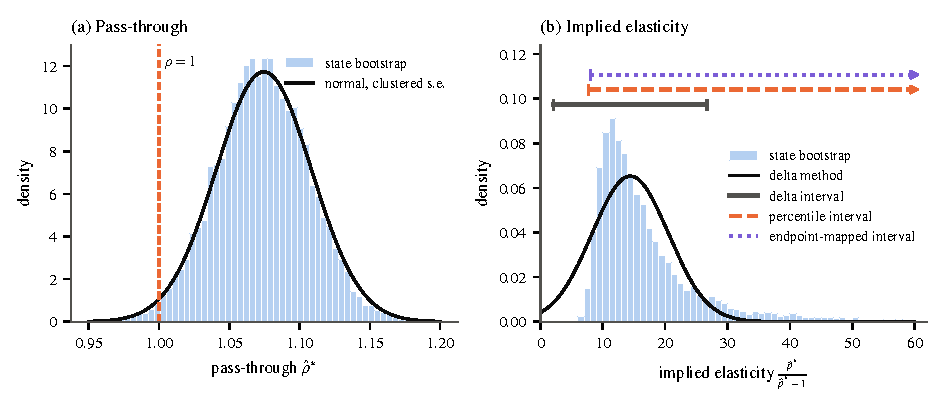
\includegraphics[width=\textwidth]{figures/appA/delta_boot.pdf}
\caption{State-cluster bootstrap of the cigarette tax pass-through regression with state and year effects. (a)
9,999 bootstrap estimates $\hat\rho^*$ and the normal density with the state-clustered standard error.
(b) Implied elasticity $\frac{\hat\rho^*}{\hat\rho^* - 1}$ and the delta-method normal density. The
horizontal bars are 95 percent intervals: delta method $[2.1, 26.7]$, bootstrap percentile $[7.7, 68.9]$, and the
mapped endpoints of the clustered interval for $\rho$, $[8.0, 162.9]$. Arrows mark intervals that extend beyond
the plotted range. 4.4 percent of the bootstrap elasticities lie outside $[0, 60]$ and are not plotted. Seed
20261022.}
\label{fig:A-delta-boot}
\end{figure}

\casehead{The Sumner panel}
We apply a pairs cluster bootstrap by state to row (1) of \cref{tab:A-sumner}, with $B = 9{,}999$. Each replication
draws 48 states with replacement, treats repeated states as distinct, and re-estimates \eqref{eq:A-sumner} with state
and year effects. The bootstrap standard error of $\hat\rho$ is 0.033, close to the clustered 0.034 and to the
jackknife value of 0.034 obtained by deleting one state at a time. \Cref{tab:A-boot-intervals} compares intervals.
For $\rho$, all methods give similar intervals that exclude one. The bootstrap distribution in
\cref{fig:A-delta-boot}(a) is close to normal, and 1.3 percent of the bootstrap estimates are at or below one.

\begin{table}[htbp]
\centering
\begin{threeparttable}
\caption{95 percent intervals for pass-through and the implied elasticity}
\label{tab:A-boot-intervals}
\small
\begin{tabular}{@{}lcc@{}}
\toprule
Method & $\rho$ & $\varepsilon = \frac{\rho}{\rho - 1}$ \\
\midrule
Clustered $t_{47}$ interval, delta method for $\varepsilon$ & $[1.006,\ 1.143]$ & $[2.1,\ 26.7]$ \\
Clustered $t_{47}$ interval, endpoints mapped & $[1.006,\ 1.143]$ & $[8.0,\ 162.9]$ \\
Bootstrap percentile & $[1.008,\ 1.137]$ & $[7.7,\ 68.9]$ \\
Bootstrap percentile for $\rho$, endpoints mapped & & $[8.3,\ 126.8]$ \\
Bootstrap basic & $[1.012,\ 1.141]$ & $[-40.1,\ 21.1]$ \\
Bootstrap percentile-$t$ & $[1.012,\ 1.143]$ & \\
Bootstrap BCa, endpoints mapped for $\varepsilon$ & $[1.012,\ 1.142]$ & $[8.0,\ 81.2]$ \\
\bottomrule
\end{tabular}
\begin{tablenotes}\footnotesize
\item Notes: Row (1) of \cref{tab:A-sumner}, $\hat\rho = 1.075$ and $\hat\varepsilon = 14.4$. Pairs cluster bootstrap
by state with 9,999 replications. The percentile-$t$ interval studentizes with the CR1 standard error in each
replication. BCa uses the jackknife over states for the acceleration ($\hat a = 0.019$, $z_0 = 0.030$).
\end{tablenotes}
\end{threeparttable}
\end{table}

For the elasticity the methods disagree sharply. Because 1.3 percent of the $\hat\rho^*$ lie below one, the same
share of bootstrap elasticities is negative and huge in magnitude. The percentile interval for $\varepsilon$ is
then not the image of the percentile interval for $\rho$. The map $\frac{\rho}{\rho - 1}$ is monotone on each side of
one, but not over the whole bootstrap support, so the transformation-respecting property fails. The basic interval
reflects the long right tail to the left and includes negative elasticities, which makes no economic sense. The
bootstrap standard deviation of the elasticity is 222, a meaningless number. The ratio has no finite moments
whenever the distribution of its denominator has positive density at zero. Intervals for $\varepsilon$ should be
built from an interval for $\rho$ and mapped through the monotone function, as in the second and last rows.

\subsection{Multi-step estimators and counterfactuals}\label{sec:A-boot-multistep}

The bootstrap's main practical advantage is that it handles estimators built in several steps. The rule is simple:
every step that uses the data must be repeated in every replication. Holding a first-step estimate fixed omits its
sampling variance, the problem that the analytical correction of \cref{prop:A-twostep} addresses. Two examples
recur in the book.

The first is a generated regressand. Marginal costs implied by a logit pricing condition, $mc_{jt} = p_{jt} -
\frac{1}{\hat\alpha(1 - S_{ft})}$, depend on the demand estimate $\hat\alpha$. Regressing them on cost shifters with
the usual standard errors treats $\hat\alpha$ as known. A market bootstrap that re-estimates $\alpha$ in each of 5,000
replications raises the standard error of the intercept from 0.016 to 0.072 in the simulated markets of
\cref{sec:C-logit-est}. The slopes barely change, because uncertainty about $\alpha$ moves all markups together.

The second is a counterfactual. \citet[WP p.~25]{ChaudhuriGoldbergJia2006} compute standard errors for counterfactual
prices and welfare losses under patent enforcement by bootstrapping the original sample 300 times. For each sample
they re-estimate the demand system and recompute the counterfactual equilibrium prices and welfare losses for each
policy scenario. When a replication's counterfactual did not converge, they compute the standard errors from the
replications that did (WP p.~25, n.~29). Dropping failed replications is common but not innocuous. If failures
occur for particular parameter values, the retained replications are a selected sample of the bootstrap distribution.

\casehead{Parametric bootstrap and parameter draws}
Two cheaper procedures are often called a parametric bootstrap, and they differ. The first simulates new data sets
from the fitted model $F(\cdot;\hat\theta)$ and re-estimates on each. It is the natural way to compute the null
distribution of a specification test whose statistic has no tractable limit. \citet[p.~241]{AtheyLevinSeira2011}
use it for the conditional Kolmogorov test of \citet{Andrews1997} and cannot reject their parametric bid model even at
the 20 percent level. The second draws parameter vectors from the estimated asymptotic distribution
$N(\hat\theta, \hat V)$ and recomputes the statistic of interest without re-estimating
(\cref{rem:A-krinsky-robb}). Athey, Levin and Seira use this second procedure for the predicted outcomes of their
Table~V (p.~248), as do \citet{Nevo2001} and \citet{Gentzkow2007}.

The validity conditions follow from what each procedure resamples. Parameter draws are valid when $\hat\theta$ is
approximately normal and $a$ is smooth. They are first-order equivalent to the delta method and cost one evaluation
of $a$ per draw. Re-estimating on resampled data also captures departures of $\hat\theta$ from normality, and it is
the only one of the three that can deliver a refinement. It is also the most expensive. \citet[p.~733,
n.~33]{Gentzkow2007} notes that bootstrapping would require estimating all parameters for each resample, which adds
greatly to the computational cost.

\subsection{When the bootstrap fails}\label{sec:A-boot-fail}

Bootstrap consistency rests on the statistic being a smooth function of the empirical distribution. Without
smoothness it can fail, and the canonical example is an extreme order statistic.

\begin{proposition}[The bootstrap of a sample maximum]\label{prop:A-boot-max}
Let $X_1, \dots, X_n$ be i.i.d.\ uniform on $[0, \theta]$ and $\hat\theta = \max_iX_i$. Then
$\frac{n(\theta - \hat\theta)}{\theta}$ converges in distribution to the standard exponential distribution, which is
continuous (\cref{prop:A-uniform-mle}). For the nonparametric bootstrap,
\begin{equation*}
  \Pr^*\bigl(\hat\theta^* = \hat\theta\bigr) = 1 - \Bigl(1 - \frac{1}{n}\Bigr)^n \longrightarrow 1 - e^{-1} \approx 0.632.
\end{equation*}
The bootstrap distribution of $\frac{n(\hat\theta - \hat\theta^*)}{\hat\theta}$ has an atom of mass about 0.632 at
zero and does not converge to the exponential limit.
\end{proposition}

\begin{proof}
The bootstrap maximum equals $\hat\theta$ if and only if the largest observation is drawn at least once. Each of the
$n$ independent draws misses it with probability $1 - \frac{1}{n}$, so it is never drawn with probability
$(1 - \frac{1}{n})^n$. Taking logs, $n\ln(1 - \frac{1}{n}) = n(-\frac{1}{n} - \frac{1}{2n^2} - \cdots) \to -1$, so
$(1 - \frac{1}{n})^n \to e^{-1}$. A limit distribution with an atom of mass $1 - e^{-1}$ at zero cannot equal the
continuous exponential distribution.
\end{proof}

The probability is already close to its limit in small samples: 0.651 for $n = 10$, 0.634 for $n = 100$ and 0.632
for $n = 1{,}000$. The intuition is that the bootstrap cannot draw values beyond the sample maximum, while the
sampling distribution of $\hat\theta$ is driven by how far the maximum falls short of the true endpoint.

The same failure appears in other non-regular problems. Parameters on the boundary of the parameter space, such as a
zero variance component, invalidate the bootstrap of the estimator \citep{Andrews2000}. Non-smooth functionals,
such as bounds formed as the maximum or minimum of estimated functions, behave like the maximum above
(\cref{sec:A-partialid}). With weak instruments the estimator is not asymptotically normal and the bootstrap does not
fix it (\cref{sec:A-weakiv}). Data with infinite variance are a further case, since the bootstrap of the sample mean
then fails. A statistic without finite moments, like the elasticity ratio above, needs a separate diagnosis. Missing
moments alone do not make the bootstrap distribution inconsistent. When the true $\rho$ is bounded away from one, the
map $\frac{\rho}{\rho - 1}$ is smooth near it. The extension of \cref{prop:A-boot-mean} to smooth functions of means
then makes the bootstrap distribution of $\sqrt n(\hat\varepsilon^* - \hat\varepsilon)$ consistent, although
$\hat\varepsilon$ has no finite moments in any finite sample. What can fail are summaries that estimate
finite-sample moments, such as the bootstrap standard deviation, because the moments they target do not exist. A true denominator at zero, or close to zero relative to its sampling error, is a
genuine non-regularity like a weak instrument. The Sumner estimate of $\rho$, about two standard errors above one, is
close to that case. Two remedies are general \citep{PolitisRomanoWolf1999}. \emph{Subsampling} recomputes the statistic on
subsamples of size $b$ drawn without replacement, with $b \to \infty$ and $\frac{b}{n} \to 0$, and rescales by the
known rate. The \emph{$m$-out-of-$n$ bootstrap} draws $m < n$ observations with replacement, with $\frac{m}{n} \to 0$.
Both work under much weaker conditions because a small subsample behaves like a fresh sample from the population.
The relevance for this book is direct. Auction models whose bid support depends on the parameters
\citep{DonaldPaarsch1996}, estimators built on extreme order statistics, and partially identified models
(\cref{ch:auction-empirics}) all fall outside the standard bootstrap's guarantees.

\section{Nonparametric estimation of distributions and densities}\label{sec:A-kde}

The estimators of the previous sections are parametric, in the sense that a finite-dimensional $\theta$ indexes
the model. Several of the book's estimators instead recover an unknown distribution without a parametric family. The
structural auction literature is the main user. The value distribution of an ascending auction is
recovered from the distribution of transaction prices. In a first-price auction it is recovered from the
distribution and density of bids (\cref{ch:auction-empirics}). Bidding
rings and procurement auctions with unobserved heterogeneity add a deconvolution step
(\cref{ch:collusion-evidence}), and hedonic demand models use nonparametric regression
(\cref{ch:discrete}). This section develops the estimators of distribution functions and densities on
which these applications rest. \Cref{sec:A-npreg} turns to regression, deconvolution and bounds.

The notation is local to these two sections. A \emph{kernel} $\mathcal{K}$ is a weighting function,
$h>0$ is a \emph{bandwidth}, and $\mathcal{K}_h(u)=\frac{1}{h}\mathcal{K}(\frac{u}{h})$. The constants
$\mu_2=\int u^2\mathcal{K}(u)\,\dd u$ and $\kappa_2=\int\mathcal{K}(u)^2\,\dd u$ are the second moment
and the roughness of the kernel, and $R$ counts the derivatives of the target function. In the auction
applications we follow \citet{GuerrePerrigneVuong2000}, hereafter GPV, and write $L$ for the number of
auctions. In these two sections $L$ is therefore neither a Lerner index nor a number of instruments. Each auction has $N$
bidders (GPV write $I$), bids are $B_{il}$, and the bid distribution and density are $G$ and $g$.

\subsection{The empirical distribution function}\label{sec:A-ecdf}

Let $X_1,\dots,X_n$ be independent draws from a distribution function $F$ on $\R$. The
\emph{empirical distribution function} puts mass $\frac{1}{n}$ on each observation:
\begin{equation}\label{eq:A-ecdf}
\hat F_n(x)=\frac{1}{n}\sum_{i=1}^{n}\indic\{X_i\le x\}.
\end{equation}

\begin{proposition}[Properties of the empirical distribution function]\label{prop:A-ecdf}
Let $X_1,\dots,X_n$ be i.i.d.\ with distribution function $F$.
\begin{enumerate}[label=(\roman*)]
\item For every $x$, $\E[\hat F_n(x)]=F(x)$ and $\Var(\hat F_n(x))=\frac{F(x)(1-F(x))}{n}$.
\item For every $x$, $\sqrt n(\hat F_n(x)-F(x))\xrightarrow{d}N(0,F(x)(1-F(x)))$.
\item (Glivenko-Cantelli) $\sup_x|\hat F_n(x)-F(x)|\to0$ almost surely.
\item (Dvoretzky-Kiefer-Wolfowitz) For every $\epsilon>0$,
$\Pr\left(\sup_x|\hat F_n(x)-F(x)|>\epsilon\right)\le2e^{-2n\epsilon^2}$.
\end{enumerate}
\end{proposition}

\begin{proof}
For fixed $x$ the indicators $\indic\{X_i\le x\}$ are i.i.d.\ Bernoulli variables with success probability
$F(x)$. Their mean is $F(x)$ and their variance is $F(x)(1-F(x))$. Averaging $n$ of them divides the
variance by $n$, which proves (i). Part (ii) is the Lindeberg-L\'evy central limit theorem applied to the
same Bernoulli average. Parts (iii) and (iv) are classical uniform results. The constant 2 in front of
the exponential in (iv) is due to \citet{Massart1990}.
\end{proof}

Part (iv) yields a confidence band that holds for all $x$ at once. Setting $2e^{-2n\epsilon^2}=\alpha$
gives $\epsilon_\alpha=\sqrt{\frac{\ln(\frac{2}{\alpha})}{2n}}$, and the band
$\hat F_n(x)\pm\epsilon_\alpha$ contains the whole function $F$ with probability at least $1-\alpha$. With
$n=200$ and $\alpha=0.05$ the half-width is about 0.096. The band needs no smoothing and no
estimate of a density, which makes the empirical distribution function the natural first step of every
estimator in this section.

\casehead{Order-statistic inversion}
In a second-price or ascending auction with symmetric independent private values, the price equals
the second-highest value (\cref{ch:auction-theory}). Suppose we observe only prices $w_l$ from $L_N$
auctions with $N$ bidders each. The price is $v_{(N-1:N)}$, and its distribution function is
\begin{equation}\label{eq:A-phiN}
F_w(v)=\Pr\left(v_{(N-1:N)}\le v\right)=\phi_N(F(v)),\qquad \phi_N(x)=Nx^{N-1}(1-x)+x^N .
\end{equation}
The second-highest value lies below $v$ exactly when at least $N-1$ of the $N$ values do. The first term
of $\phi_N$ is the probability that exactly $N-1$ values lie below $v$, and the second that all $N$ do.
The derivative is
\begin{equation*}
\phi_N'(x)=N(N-1)x^{N-2}(1-x)-Nx^{N-1}+Nx^{N-1}=N(N-1)x^{N-2}(1-x),
\end{equation*}
which is positive on $(0,1)$. So $\phi_N$ is a strictly increasing bijection of $[0,1]$, and
$F(v)=\phi_N^{-1}(F_w(v))$. More generally, the $k$-th lowest of $N$ i.i.d.\ draws has distribution
function
\begin{equation}\label{eq:A-orderstat}
F_{(k:N)}(v)=\frac{N!}{(N-k)!\,(k-1)!}\int_0^{F(v)}t^{k-1}(1-t)^{N-k}\,\dd t ,
\end{equation}
which is strictly increasing in $F(v)$ \citep[eq.~(5)]{AtheyHaile2002}. Any single order statistic with
known $N$ therefore identifies $F$, and \eqref{eq:A-phiN} is the case $k=N-1$.

The plug-in estimator replaces $F_w$ by the empirical distribution function of the prices,
$\hat F(v)=\phi_N^{-1}(\hat F_w(v))$, computed by bisection at each $v$.

\begin{proposition}[Order-statistic inversion]\label{prop:A-os-inversion}
Let $w_1,\dots,w_{L_N}$ be i.i.d.\ prices from $N$-bidder auctions and let $0<F(v)<1$. Then
$\hat F(v)\xrightarrow{p}F(v)$ and
\begin{equation}\label{eq:A-os-avar}
\sqrt{L_N}\left(\hat F(v)-F(v)\right)\xrightarrow{d}
N\!\left(0,\ \frac{F_w(v)(1-F_w(v))}{\phi_N'(F(v))^2}\right).
\end{equation}
\end{proposition}

\begin{proof}
Consistency follows from \cref{prop:A-ecdf}(i) and the continuity of $\phi_N^{-1}$. The inverse
function theorem gives $\frac{\dd}{\dd y}\phi_N^{-1}(y)=\frac{1}{\phi_N'(\phi_N^{-1}(y))}$, which is
finite because $\phi_N'(F(v))>0$. The delta method (\cref{thm:A-delta}) applied to
\cref{prop:A-ecdf}(ii) multiplies the asymptotic variance $F_w(1-F_w)$ by the square of this
derivative.
\end{proof}

The variance in \eqref{eq:A-os-avar} measures what is lost by observing one order statistic. If all $N$
values of each auction were recorded, the empirical distribution function of the $NL_N$ values would
have asymptotic variance $\frac{F(1-F)}{N}$ per auction. With $N=4$ and $F(v)=0.5$, the price-only
variance is 0.0955 against 0.0625, a ratio of 1.53. At $F(v)=0.2$ the ratio is 4.49, and with $N=6$ at
the same point it reaches 40.6. The price is the second-highest value, so it carries little information about the lower
tail, and the loss grows with $N$. These numbers come from \texttt{kernel\_constants.py}.

Two extensions matter in practice. First, the inversion delivers one estimate of $F$ for each $N$ in the
data. If participation varies independently of values, all these estimates must coincide, which is a
testable restriction \citep[Theorem~1]{AtheyHaile2002}. The estimates from different $N$ are
independent, so a Wald-type comparison at a point $v$ divides their difference by the square root of the
sum of the two variances in \eqref{eq:A-os-avar}. Second, with a binding reserve price $r$ the price is
$\max\{v_{(N-1:N)},r\}$, and $F$ is identified only above $r$. \Cref{ch:auction-empirics} develops the
identification argument, and \cref{sec:A-partialid} returns to ascending auctions in which recorded bids
are not values.

\subsection{The kernel density estimator}\label{sec:A-kde-estimator}

A histogram estimates a density by counting observations in bins of width $2h$. It depends on the bin
origin, and it is discontinuous. The kernel estimator centers a smooth bump on each observation
instead \citep{Rosenblatt1956,Parzen1962}:
\begin{equation}\label{eq:A-kde}
\hat f_h(x)=\frac{1}{nh}\sum_{i=1}^{n}\mathcal{K}\!\left(\frac{x-X_i}{h}\right)
=\frac{1}{n}\sum_{i=1}^{n}\mathcal{K}_h(x-X_i).
\end{equation}
With the uniform kernel $\mathcal{K}(u)=\frac{1}{2}\indic\{|u|\le1\}$, $\hat f_h(x)$ is the share of
observations within $h$ of $x$ divided by $2h$, a histogram whose bin moves with $x$.

\begin{definition}[Second-order kernel]\label{def:A-kernel}
A \emph{second-order kernel} is a bounded function $\mathcal{K}$ with $\int\mathcal{K}(u)\,\dd u=1$,
$\int u\mathcal{K}(u)\,\dd u=0$, $0<\mu_2=\int u^2\mathcal{K}(u)\,\dd u<\infty$ and
$\kappa_2=\int\mathcal{K}(u)^2\,\dd u<\infty$. A bounded symmetric density with finite variance is a
second-order kernel.
\end{definition}

\begin{assumption}[Pointwise kernel asymptotics]\label{ass:A-kde}
The draws $X_1,\dots,X_n$ are i.i.d.\ with density $f$. In a neighborhood of the point $x$, $f$ is twice
continuously differentiable with bounded second derivative. The kernel is second order, and the bandwidth
satisfies $h\to0$ and $nh\to\infty$.
\end{assumption}

\begin{proposition}[Bias and variance of the kernel density estimator]\label{prop:A-kde-bias-var}
Under \cref{ass:A-kde},
\begin{equation}\label{eq:A-kde-bias-var}
\E[\hat f_h(x)]-f(x)=\frac{h^2}{2}\mu_2f''(x)+o(h^2),\qquad
\Var(\hat f_h(x))=\frac{f(x)\kappa_2}{nh}+o\!\left(\frac{1}{nh}\right).
\end{equation}
\end{proposition}

\begin{proof}
\emph{Bias.} The summands of \eqref{eq:A-kde} are i.i.d., so
\begin{equation*}
\E[\hat f_h(x)]=\int\frac{1}{h}\mathcal{K}\!\left(\frac{x-y}{h}\right)f(y)\,\dd y
=\int\mathcal{K}(u)f(x-hu)\,\dd u ,
\end{equation*}
where we substituted $y=x-hu$ and $\dd y=-h\,\dd u$. A second-order Taylor expansion with mean-value
point $\tilde x_u$ between $x$ and $x-hu$ gives
\begin{equation*}
f(x-hu)=f(x)-huf'(x)+\frac{h^2u^2}{2}f''(\tilde x_u).
\end{equation*}
Integrating against $\mathcal{K}$, the first term returns $f(x)$ and the second vanishes because
$\int u\mathcal{K}=0$. The third equals $\frac{h^2}{2}\int u^2\mathcal{K}(u)f''(\tilde x_u)\,\dd u$, which
is $\frac{h^2}{2}\mu_2f''(x)+o(h^2)$ by continuity of $f''$ and dominated convergence.

\emph{Variance.} Again by independence,
\begin{equation*}
\Var(\hat f_h(x))=\frac{1}{n}\left\{\E\left[\mathcal{K}_h(x-X)^2\right]-\left(\E[\mathcal{K}_h(x-X)]\right)^2\right\}.
\end{equation*}
The same substitution gives
$\E[\mathcal{K}_h(x-X)^2]=\frac{1}{h}\int\mathcal{K}(u)^2f(x-hu)\,\dd u=\frac{f(x)\kappa_2}{h}+O(1)$.
The squared mean is $f(x)^2+O(h^2)=O(1)$. Hence
$\Var(\hat f_h(x))=\frac{f(x)\kappa_2}{nh}+O(\frac{1}{n})$, and $\frac{1}{n}=o(\frac{1}{nh})$ because
$h\to0$.
\end{proof}

The proposition displays the basic trade-off of nonparametric estimation. A small bandwidth averages
few observations, so the variance is large. A large bandwidth averages over a region where $f$ curves,
so the bias is large. The variance is of order $\frac{1}{nh}$ because only about $2nhf(x)$ observations
fall in the kernel window, which is slower than the parametric $\frac{1}{n}$. Under the same conditions
a Lindeberg argument gives
$\sqrt{nh}\,(\hat f_h(x)-\E[\hat f_h(x)])\xrightarrow{d}N(0,f(x)\kappa_2)$.

\casehead{Optimal bandwidth}
The \emph{mean integrated squared error} is
$\mathrm{MISE}(h)=\E\int(\hat f_h(x)-f(x))^2\,\dd x$, the integral of squared bias plus variance.
Integrating the leading terms of \eqref{eq:A-kde-bias-var} and using $\int f=1$ gives the
\emph{asymptotic MISE}
\begin{equation}\label{eq:A-amise}
\mathrm{AMISE}(h)=\frac{h^4}{4}\mu_2^2\,\mathcal{R}(f'')+\frac{\kappa_2}{nh},\qquad
\mathcal{R}(f'')=\int f''(x)^2\,\dd x .
\end{equation}
The first-order condition $h^3\mu_2^2\mathcal{R}(f'')-\frac{\kappa_2}{nh^2}=0$ yields
\begin{equation}\label{eq:A-hstar}
h^*=\left[\frac{\kappa_2}{\mu_2^2\,\mathcal{R}(f'')\,n}\right]^{\frac{1}{5}} .
\end{equation}
At $h^*$ the squared-bias term equals one quarter of the variance term, so
\begin{equation*}
\mathrm{AMISE}(h^*)=\frac{5}{4}\,\frac{\kappa_2}{nh^*}
=\frac{5}{4}\left(\sqrt{\mu_2}\,\kappa_2\right)^{\frac{4}{5}}\mathcal{R}(f'')^{\frac{1}{5}}\,n^{-\frac{4}{5}} .
\end{equation*}
The optimal bandwidth shrinks like $n^{-\frac{1}{5}}$ and the error falls like $n^{-\frac{4}{5}}$, against
$n^{-1}$ for a correctly specified parametric model.

\casehead{Silverman's rule of thumb}
The unknown $\mathcal{R}(f'')$ in \eqref{eq:A-hstar} can be replaced by its value for a reference
density. Take $f$ normal with variance $\sigma^2$ and the Gaussian kernel, for which $\mu_2=1$ and
$\kappa_2=\frac{1}{2\sqrt\pi}$. Write $f(x)=\frac{1}{\sigma}\phi(\frac{x}{\sigma})$ with $\phi$ the
standard normal density. Then $f''(x)=\sigma^{-3}\phi''(\frac{x}{\sigma})$ and
$\phi''(u)=(u^2-1)\phi(u)$, so
\begin{equation*}
\mathcal{R}(f'')=\sigma^{-5}\int(u^2-1)^2\phi(u)^2\,\dd u .
\end{equation*}
Now $\phi(u)^2=\frac{1}{2\sqrt\pi}\,\psi(u)$, where $\psi$ is the $N(0,\frac{1}{2})$ density. For
$U\sim N(0,\frac{1}{2})$ we have $\E[U^2]=\frac{1}{2}$ and $\E[U^4]=\frac{3}{4}$, so
$\E[(U^2-1)^2]=\frac{3}{4}-1+1=\frac{3}{4}$. Therefore
\begin{equation*}
\mathcal{R}(f'')=\frac{3}{8\sqrt\pi\,\sigma^5},\qquad
(h^*)^5=\frac{\frac{1}{2\sqrt\pi}}{\frac{3}{8\sqrt\pi\,\sigma^5}\,n}=\frac{4}{3}\,\frac{\sigma^5}{n},
\end{equation*}
and
\begin{equation}\label{eq:A-silverman}
h_{\mathrm{ROT}}=\left(\frac{4}{3}\right)^{\frac{1}{5}}\sigma n^{-\frac{1}{5}}\approx1.06\,\sigma n^{-\frac{1}{5}} .
\end{equation}
This is the \emph{rule of thumb} of \citet{Silverman1986}, with $\sigma$ replaced by the sample standard
deviation. It is optimal for normal data and oversmooths densities with more curvature, such as
multimodal ones, because those have larger $\mathcal{R}(f'')$.

\casehead{Choice of kernel}
The kernel enters \eqref{eq:A-hstar} only through $\delta_{\mathcal{K}}=(\frac{\kappa_2}{\mu_2^2})^{\frac{1}{5}}$,
and the minimized AMISE only through $\sqrt{\mu_2}\,\kappa_2$. Two consequences follow. A bandwidth
rule derived for one kernel converts to another kernel by the factor
$\frac{\delta_{\mathcal{K}}}{\delta_{\phi}}$, whatever $f$ is. And kernels differ little in efficiency
once their bandwidths are scaled correctly. \Cref{tab:A-kernels} reports the constants. Among nonnegative
kernels the Epanechnikov kernel minimizes $\sqrt{\mu_2}\,\kappa_2$, and every other kernel in the table
attains at least 92.9 percent of its efficiency. The restriction to nonnegative kernels matters, because
\cref{def:A-kernel} allows negative values. Put weight $\lambda$ on the Epanechnikov kernel and $1 - \lambda$
on a bounded kernel of order four with compact support (\cref{sec:A-kde-higher}). The mixture is a second-order
kernel with $\mu_2 = \frac{\lambda}{5}$ and bounded $\kappa_2$, so its criterion tends to zero as $\lambda \to 0$.

\begin{table}[htbp]
\centering
\caption{Second-order kernels and their constants}\label{tab:A-kernels}
\begin{tabular}{lccccccc}
\toprule
Kernel & $\mathcal{K}(u)$ & $\mu_2$ & $\kappa_2$ & $\int\mathcal{K}'(u)^2\dd u$ & $\int_0^\infty u\mathcal{K}(u)\dd u$
 & $\frac{\delta_{\mathcal{K}}}{\delta_\phi}$ & Efficiency \\
\midrule
Uniform & $\frac{1}{2}$ & $\frac{1}{3}$ & $\frac{1}{2}$ & n.a. & $\frac{1}{4}$ & 1.740 & 0.930 \\[2pt]
Epanechnikov & $\frac{3}{4}(1-u^2)$ & $\frac{1}{5}$ & $\frac{3}{5}$ & $\frac{3}{2}$ & $\frac{3}{16}$ & 2.214 & 1.000 \\[2pt]
Biweight & $\frac{15}{16}(1-u^2)^2$ & $\frac{1}{7}$ & $\frac{5}{7}$ & $\frac{15}{7}$ & $\frac{5}{32}$ & 2.623 & 0.994 \\[2pt]
Triweight & $\frac{35}{32}(1-u^2)^3$ & $\frac{1}{9}$ & $\frac{350}{429}$ & $\frac{35}{11}$ & $\frac{35}{256}$ & 2.978 & 0.987 \\[2pt]
Gaussian & $\phi(u)$ & $1$ & $\frac{1}{2\sqrt\pi}$ & $\frac{1}{4\sqrt\pi}$ & $\frac{1}{\sqrt{2\pi}}$ & 1.000 & 0.951 \\
\bottomrule
\end{tabular}
\par\smallskip
\begin{minipage}{0.97\textwidth}
\footnotesize Notes: the first four kernels are zero outside $|u|\le1$. The column
$\frac{\delta_{\mathcal{K}}}{\delta_\phi}$ is the factor that converts a bandwidth rule for the Gaussian
kernel into the corresponding rule for kernel $\mathcal{K}$, with
$\delta_{\mathcal{K}}=(\frac{\kappa_2}{\mu_2^2})^{\frac{1}{5}}$. Efficiency is $\sqrt{\mu_2}\,\kappa_2$ of
the Epanechnikov kernel divided by $\sqrt{\mu_2}\,\kappa_2$ of the kernel in the row. It is the ratio of
sample sizes that gives the two kernels the same minimized AMISE. The
derivative roughness $\int\mathcal{K}'^2$ enters the variance of density-derivative estimators
(\cref{prop:A-kde-derivative}). The uniform kernel is not differentiable. All constants are computed
exactly with sympy in \texttt{kernel\_constants.py}.
\end{minipage}
\end{table}

The auction literature uses the triweight kernel almost exclusively. It has compact support, so
trimmed observations drop out of the estimate, and it is continuously differentiable on the whole line,
including the end points of its support. \citet[p.~532]{GuerrePerrigneVuong2000} chose it to satisfy
their kernel assumptions. \citet[p.~180]{LiPerrigneVuong2002} and \citet[Section~4.3]{Krasnokutskaya2011}\footnote{We use the
working-paper version of \citet{Krasnokutskaya2011} dated May 24, 2004 (PIER Working Paper 05-006), and equation,
section, lemma and proposition numbers refer to it.}
give the differentiability at the boundary as the reason. These authors also illustrate the conversion
factor. \citeauthor{LiPerrigneVuong2002} and \citeauthor{Krasnokutskaya2011} set the bandwidth constant
to $2.978\times1.06\,\hat\sigma$, and 2.978 is the triweight entry in the
$\frac{\delta_{\mathcal{K}}}{\delta_\phi}$ column. \citet[p.~532]{GuerrePerrigneVuong2000} and
\citet[p.~749]{Asker2010} use $1.06\,\hat\sigma$ with the same kernel, a bandwidth about one third of the
normal-reference rule for that kernel.

The exponents of the sample size also differ across these papers. GPV set $h_g=1.06\,\hat\sigma_b(NL)^{-\frac{1}{5}}$
for the bid density, with $\hat\sigma_b$ the standard deviation of the bids and $NL$ the number of bids (p.~532).
\citet[p.~749]{Asker2010} uses $1.06\,\hat\sigma n^{-\frac{1}{6}}$ for densities and $1.06\,\hat\sigma n^{-\frac{1}{5}}$
for kernel-smoothed distribution functions. \citet[Section~4.3]{Krasnokutskaya2011} uses
$2.978\times1.06\,\hat\sigma L^{-\frac{1}{6}}$, with $L$ her sample size and $\hat\sigma$ the standard deviation of
the log of one plus the bids, and says that she follows GPV. The rates of \cref{sec:A-kde-higher} explain the pattern. With $R$
derivatives of the value density and $d$ continuous covariates, GPV's bandwidths for the bid distribution and the bid
density shrink like $L^{-\frac{1}{2R+d+2}}$ and $L^{-\frac{1}{2R+d+3}}$, up to logarithms. With $R=1$ and no
covariates the density exponent is $-\frac{1}{5}$, GPV's own choice. With $R=1$ and $d=1$ the two exponents are
$-\frac{1}{5}$ and $-\frac{1}{6}$, the pair that Asker uses. Neither Asker nor Krasnokutskaya derives an exponent. In a
one-dimensional problem $L^{-\frac{1}{6}}$ shrinks more slowly than $L^{-\frac{1}{5}}$, so their bandwidths oversmooth
slightly relative to GPV's rule. Oversmoothing lowers the variance of $\hat g$ at the cost of more bias.

\Cref{fig:A-kde} illustrates the trade-off with a bimodal density,
$f=0.6\,N(0,1)+0.4\,N(2.5,0.5^2)$, and $n=200$. Panel (a) shows one sample. Halving the optimal
bandwidth produces spurious bumps, and doubling it blurs the two modes into a plateau. Panel (b) plots
the exact integrated squared bias, integrated variance and MISE against $h$, with Monte Carlo averages
over 1,000 samples as markers. The exact MISE is minimized at $h^*=0.291$, where the integrated
squared bias is 0.0014 and the integrated variance 0.0039. The AMISE formula \eqref{eq:A-hstar} gives
0.262. Its quartic bias term overstates the bias at large $h$, which pulls the AMISE minimizer to the
left.

\begin{figure}[htbp]
\centering
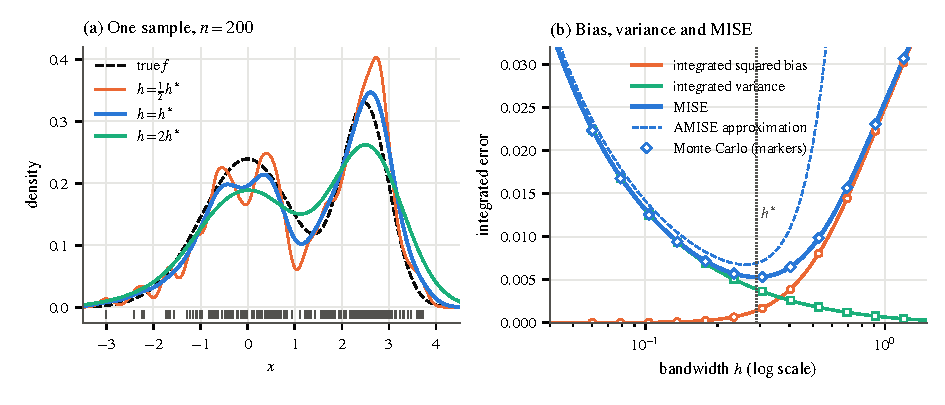
\includegraphics[width=\textwidth]{figures/appA/kde.pdf}
\caption{Bandwidth choice for a kernel density estimator. The true density is
$0.6\,N(0,1)+0.4\,N(2.5,0.5^2)$, the kernel is Gaussian and $n=200$. (a) One sample (the
median of 101 fresh samples by integrated squared error at $h^*$), with estimates at
$\frac{1}{2}h^*$, $h^*$ and $2h^*$, where $h^*=0.291$ minimizes the exact MISE. (b) Exact
integrated squared bias, integrated variance and MISE (solid lines), the AMISE approximation
\eqref{eq:A-amise} (dashed) and Monte Carlo averages over 1,000 samples (markers). Seed 20261022,
script \texttt{kde\_demo.py}.}
\label{fig:A-kde}
\end{figure}

\subsection{Smoothness, higher-order kernels and derivatives}\label{sec:A-kde-higher}

The $h^2$ bias of \cref{prop:A-kde-bias-var} comes from the second moment of the kernel. If $f$ has more
derivatives, kernels with more vanishing moments reduce the bias further.

\begin{definition}[Kernel of order $R$]\label{def:A-kernel-order}
A kernel $\mathcal{K}$ is of \emph{order} $R\ge2$ if $\int\mathcal{K}=1$,
$\mu_j=\int u^j\mathcal{K}(u)\,\dd u=0$ for $j=1,\dots,R-1$, and $0<|\mu_R|<\infty$.
\end{definition}

If $f$ has $R$ bounded continuous derivatives near $x$ and $\mathcal{K}$ is of order $R$, the expansion in
the proof of \cref{prop:A-kde-bias-var}, carried to order $R$, gives
\begin{equation}\label{eq:A-kde-bias-R}
\E[\hat f_h(x)]-f(x)=\sum_{j=1}^{R}\frac{(-h)^j}{j!}\mu_jf^{(j)}(x)+o(h^R)
=\frac{(-h)^R}{R!}\mu_Rf^{(R)}(x)+o(h^R).
\end{equation}
The variance is unchanged at order $\frac{1}{nh}$. Balancing $h^{2R}$ against $\frac{1}{nh}$ gives
$h\propto n^{-\frac{1}{2R+1}}$ and a root mean squared error of order $n^{-\frac{R}{2R+1}}$.
\citet{Stone1982} showed that $(\frac{n}{\log n})^{\frac{R}{2R+1}}$ is the best possible rate for
estimating such a density uniformly over a compact set. The logarithm is the price of uniformity.

For $R>2$ the kernel must take negative values, since $\mu_2=0$ is impossible for a nonnegative
function. Density estimates can then be negative. In the auction setting this has a concrete cost. A
negative estimated bid density produces pseudo-values below the corresponding bids, so
\citet[p.~180]{LiPerrigneVuong2002} keep second-order kernels in their three-bidder design even though
their theory calls for order three.

\casehead{Derivatives of a density}
Differentiating \eqref{eq:A-kde} gives an estimator of the derivative,
\begin{equation}\label{eq:A-kde-deriv}
\hat f_h'(x)=\frac{1}{nh^2}\sum_{i=1}^{n}\mathcal{K}'\!\left(\frac{x-X_i}{h}\right).
\end{equation}

\begin{proposition}[Rate for a density derivative]\label{prop:A-kde-derivative}
Let $\mathcal{K}$ be a continuously differentiable kernel of order $R$ that vanishes outside $[-1,1]$, and
let $f$ have $R+1$ bounded continuous derivatives near $x$. If $h\to0$ and $nh^3\to\infty$, then
\begin{equation*}
\E[\hat f_h'(x)]-f'(x)=\frac{(-h)^R}{R!}\mu_Rf^{(R+1)}(x)+o(h^R),\qquad
\Var(\hat f_h'(x))=\frac{f(x)\int\mathcal{K}'(u)^2\dd u}{nh^3}+o\!\left(\frac{1}{nh^3}\right).
\end{equation*}
The mean squared error is minimized by $h\propto n^{-\frac{1}{2R+3}}$, and the root mean squared error is
then of order $n^{-\frac{R}{2R+3}}$.
\end{proposition}

\begin{proof}
\emph{Bias.} Substituting $y=x-hu$,
\begin{equation*}
\E[\hat f_h'(x)]=\frac{1}{h}\int\mathcal{K}'(u)f(x-hu)\,\dd u .
\end{equation*}
Integration by parts, with $\mathcal{K}(\pm1)=0$ and $\frac{\dd}{\dd u}f(x-hu)=-hf'(x-hu)$, turns this into
$\int\mathcal{K}(u)f'(x-hu)\,\dd u$. This is the expectation of a kernel estimator of $f'$, and
\eqref{eq:A-kde-bias-R} applied to $f'$ gives the bias.

\emph{Variance.} Each summand of \eqref{eq:A-kde-deriv} is $\frac{1}{h^2}\mathcal{K}'(\frac{x-X_i}{h})$.
Its second moment is
\begin{equation*}
\frac{1}{h^4}\int\mathcal{K}'\!\left(\frac{x-y}{h}\right)^2f(y)\,\dd y=\frac{1}{h^3}\int\mathcal{K}'(u)^2f(x-hu)\,\dd u
=\frac{f(x)\int\mathcal{K}'^2}{h^3}+o\!\left(\frac{1}{h^3}\right),
\end{equation*}
while its squared mean is $O(1)$. Dividing by $n$ gives the variance.

\emph{Rate.} The mean squared error is $c_1h^{2R}+\frac{c_2}{nh^3}$ to first order. Its minimizer solves
$2Rc_1h^{2R-1}=\frac{3c_2}{nh^4}$, so $h\propto n^{-\frac{1}{2R+3}}$. Substituting back gives a mean
squared error of order $n^{-\frac{2R}{2R+3}}$.
\end{proof}

The variance of a derivative estimate is larger by a factor $h^{-2}$, because differentiating the kernel
divides by $h$ once more. Every additional derivative costs two more powers of $h$ in the variance and
slows the rate.

\casehead{Why first-price auctions converge slowly}
The derivative result explains the rate of the estimator of \citet{GuerrePerrigneVuong2000}. In the
symmetric IPV first-price auction with $N$ bidders, the inverse bid function is
\begin{equation}\label{eq:A-gpv-xi}
\xi(b)=b+\frac{G(b)}{(N-1)g(b)},
\end{equation}
and the value distribution satisfies $G(b)=F(\xi(b))$ (\cref{ch:auction-empirics}). Differentiating
gives $g(b)=f(\xi(b))\,\xi'(b)$, so the value density is
\begin{equation}\label{eq:A-gpv-f}
f(v)=\frac{g(\xi^{-1}(v))}{\xi'(\xi^{-1}(v))},\qquad
\xi'(b)=\frac{N}{N-1}-\frac{G(b)\,g'(b)}{(N-1)\,g(b)^2}
\end{equation}
\citep[eq.~(11)]{GuerrePerrigneVuong2000}. The value density depends on the derivative of the bid
density. GPV show that if $f$ has $R$ bounded continuous derivatives, then $g$ has $R+1$ in the
interior of its support \citep[Proposition~1]{GuerrePerrigneVuong2000}. Estimating $g'$ is then the
problem of \cref{prop:A-kde-derivative}, with $R$ derivatives of $g'$ available, and the best rate is
$n^{-\frac{R}{2R+3}}$.

GPV make this heuristic exact. With $d$ continuous auction covariates and $L$ auctions, no estimator of
the value density converges uniformly faster than $(\frac{L}{\log L})^{\frac{R}{2R+d+3}}$
\citep[Theorem~2]{GuerrePerrigneVuong2000}. If values were observed, the best rate would be
$(\frac{L}{\log L})^{\frac{R}{2R+d+1}}$. Their two-step estimator attains the bound
\citep[Theorem~3]{GuerrePerrigneVuong2000} with bandwidths $h_G\propto(\frac{\log L}{L})^{\frac{1}{2R+d+2}}$
for the distribution, $h_g\propto(\frac{\log L}{L})^{\frac{1}{2R+d+3}}$ for the bid density, and
$h_f\propto(\frac{\log L}{L})^{\frac{1}{2R+d+3}}$ for the value density (their Assumption~A4). The
first-step bandwidths are the optimal ones for $G$ and $g$. The second-step bandwidth $h_f$ is larger
than the optimal bandwidth for observed values. GPV show that this oversmoothing is the only choice
that attains the optimal rate given the first step. Pseudo-values away from the boundary converge
uniformly at the faster rate $(\frac{L}{\log L})^{\frac{R+1}{2R+d+3}}$ of $\hat g$ (their
Proposition~3), and the second step loses one power of the bandwidth when it smooths them.

\subsection{Boundary bias and trimming}\label{sec:A-kde-boundary}

Kernel estimators are biased near the edge of the support. Bid and value distributions have compact
supports, so this bias matters in every auction application.

\begin{proposition}[Boundary bias]\label{prop:A-kde-boundary}
Let $f$ be zero below $\underline x$ and continuous on $[\underline x,\underline x+\eta)$ for some
$\eta>0$, with right limit $f(\underline x^+)>0$. Let $\mathcal{K}$ be a kernel that vanishes outside
$[-1,1]$, and evaluate the estimator at $x=\underline x+ch$ with fixed $c\in[0,1)$. Then as $h\to0$,
\begin{equation*}
\E[\hat f_h(\underline x+ch)]\to f(\underline x^+)\int_{-1}^{c}\mathcal{K}(u)\,\dd u .
\end{equation*}
For a symmetric kernel the limit at the boundary point itself ($c=0$) is $\frac{1}{2}f(\underline x^+)$.
\end{proposition}

\begin{proof}
As in \cref{prop:A-kde-bias-var}, $\E[\hat f_h(x)]=\int\mathcal{K}(u)f(x-hu)\,\dd u$. The density is zero
unless $x-hu\ge\underline x$, that is, unless $u\le c$. Hence
$\E[\hat f_h(x)]=\int_{-1}^{c}\mathcal{K}(u)f(\underline x+h(c-u))\,\dd u$. As $h\to0$ the argument of $f$
converges to $\underline x$ from above, and dominated convergence gives the limit. Symmetry gives
$\int_{-1}^{0}\mathcal{K}=\frac{1}{2}$.
\end{proof}

The estimator does not converge to $f$ anywhere in the boundary region of width $h$. Dividing by the
known mass $\int_{-1}^{c}\mathcal{K}$ removes the leading term but leaves a bias of order $h$, against
$h^2$ in the interior. Applied researchers use five remedies.
\begin{enumerate}[label=(\alph*)]
\item \emph{Reflection} adds the mirror image of the sample around $\underline x$,
$\hat f_R(x)=\hat f_h(x)+\hat f_h(2\underline x-x)$ for $x\ge\underline x$. It removes the order-one
bias. A bias of order $h$ remains unless $f'(\underline x^+)=0$.
\item \emph{Boundary kernels} change shape near the edge so that their moments of order zero and one
over the available support are one and zero.
\item \emph{Transformation} estimates the density of a transformed variable whose support is
unbounded and maps back by the change-of-variables formula. \citet[footnote~13]{LiPerrigneVuong2002}
recommend $\log(1+b)$ when bids are very skewed.
\item \emph{Local linear density estimation} applies the boundary property of local linear regression
(\cref{prop:A-loclin}) to a smoothed empirical distribution function.
\item \emph{Trimming} discards estimates within a bandwidth of the edge.
\end{enumerate}

\casehead{Trimming in the GPV estimator}
GPV trim. Let $\rho_g$ be the length of the support of the kernel used for $\hat g$, so $\rho_g=2$ for
the triweight kernel. By \cref{prop:A-kde-boundary}, $\hat g$ is asymptotically biased within
$\frac{\rho_gh_g}{2}$ of either end of the bid support. Since the minimum and maximum bids converge to the
end points, GPV define the pseudo-value
\begin{equation}\label{eq:A-gpv-trim}
\hat V_{il}=\begin{cases}
B_{il}+\dfrac{\hat G(B_{il})}{(N-1)\,\hat g(B_{il})} & \text{if } B_{\min}+\frac{\rho_gh_g}{2}\le B_{il}\le B_{\max}-\frac{\rho_gh_g}{2},\\[6pt]
+\infty & \text{otherwise}
\end{cases}
\end{equation}
\citep[eq.~(6)]{GuerrePerrigneVuong2000}. With the triweight kernel the bids within $h_g$ of the extreme
bids are trimmed. An infinite pseudo-value contributes nothing to a second-step kernel estimate with
compact support, so the device trims without changing the formula. With covariates, GPV trim
observations within twice the bandwidths of the estimated boundary of the conditional support (their
eq.~(19)). \citet[eq.~(14)]{LiPerrigneVuong2002} use the window $[h_g,b_{\max}-h_g]$, since bids in their
design are bounded below by zero, and \citet[p.~749]{Asker2010} follows the same practice. Trimming has
a cost. The value density is estimated consistently only on an inner compact subset of its support, and
the second-step estimate is itself biased within $h_f$ of the trimmed region. \citet{HickmanHubbard2015}
propose boundary-corrected kernels for both steps in place of trimming.

\subsection{Bandwidth choice and inference}\label{sec:A-kde-bandwidth}

Three families of bandwidth selectors are in use. The rule of thumb \eqref{eq:A-silverman} is simple
and stable but oversmooths curved densities. \emph{Plug-in} selectors estimate $\mathcal{R}(f'')$ with
a pilot kernel estimate and insert it into \eqref{eq:A-hstar} \citep{SheatherJones1991}.
\emph{Least-squares cross-validation} (LSCV) estimates the integrated squared error directly. Expanding
the square,
\begin{equation*}
\int(\hat f_h-f)^2=\int\hat f_h^2-2\int\hat f_hf+\int f^2 .
\end{equation*}
The last term does not depend on $h$. The middle term is $2\E_X[\hat f_h(X)]$ for a new draw $X$, which
the leave-one-out average estimates without bias. The criterion is
\begin{equation}\label{eq:A-lscv}
\mathrm{CV}(h)=\int\hat f_h(x)^2\,\dd x-\frac{2}{n}\sum_{i=1}^{n}\hat f_{h,-i}(X_i),\qquad
\hat f_{h,-i}(x)=\frac{1}{(n-1)h}\sum_{j\ne i}\mathcal{K}\!\left(\frac{x-X_j}{h}\right).
\end{equation}
For the Gaussian kernel the first term has a closed form,
$\int\hat f_h^2=\frac{1}{n^2h}\sum_i\sum_j\phi_{\sqrt2}(\frac{X_i-X_j}{h})$, where $\phi_{\sqrt2}$ is the
$N(0,2)$ density, because the convolution of two standard normal densities is the $N(0,2)$ density.

The design of \cref{fig:A-kde} shows the trade-offs (\texttt{kde\_demo.py}, 1,000 samples). The
population rule of thumb is 0.545, almost twice $h^*=0.291$, because the mixture is bimodal. Its mean
integrated squared error is 0.0103, about twice the 0.0053 attained at $h^*$. LSCV is centered
correctly, with a mean of 0.294, but it is variable, with 10th and 90th percentiles of 0.199 and 0.376.
Its mean integrated squared error is 0.0067.

\casehead{Inference}
Pointwise confidence intervals rest on the normal limit of \cref{sec:A-kde-estimator}. At a bandwidth
of order $n^{-\frac{1}{5}}$ the bias is of the same order as the standard deviation. Indeed,
$\sqrt{nh}\cdot h^2=\sqrt{nh^5}$ is bounded away from zero at such a bandwidth. An interval
$\hat f_h(x)\pm1.96\sqrt{\frac{\hat f_h(x)\kappa_2}{nh}}$ is then centered at the wrong point, and its
coverage falls short of 95 percent. Two fixes are available. \emph{Undersmoothing} takes
$h=o(n^{-\frac{1}{5}})$ so that the bias vanishes relative to the standard deviation, at the cost of
wider intervals. \emph{Robust bias correction} subtracts an estimate of the bias and inflates the
standard error to account for the estimated bias \citep{CalonicoCattaneoFarrell2018}.

Auction applications rarely follow either route. \citet[Section~3.2.1, p.~21]{AtheyHaile2007} report
that data-driven bandwidth selection had not been explored there and that the asymptotic distribution of
the two-step density estimator was largely unresolved.\footnote{We read the manuscript of May 6, 2005 of
\citet{AtheyHaile2007}. Section, page, equation and footnote numbers refer to that manuscript and may
differ from the published chapter. Its assessment of the literature dates from 2005.} For functionals
that are asymptotically normal, such as quantiles of the value distribution, \citet{HaileHongShum2003}
establish normality, and practitioners bootstrap. Bids within an auction may be dependent, so outside
the independent private values model the bootstrap resamples whole auctions
\citep[Section~3.2.1, p.~21]{AtheyHaile2007}. \citet{Asker2010} resamples auctions with 5,000
iterations (\cref{sec:A-boot-dependent} develops the cluster bootstrap).

\subsection{Multivariate and conditional densities}\label{sec:A-kde-multi}

With $d$-dimensional data the product kernel estimator is
\begin{equation}\label{eq:A-kde-multi}
\hat f_h(x)=\frac{1}{nh^d}\sum_{i=1}^{n}\prod_{k=1}^{d}\mathcal{K}\!\left(\frac{x_k-X_{ik}}{h}\right).
\end{equation}
The bias is still of order $h^2$. The variance becomes $\frac{f(x)\kappa_2^d}{nh^d}$ to first order,
because the second moment of one summand is
$\frac{1}{h^{2d}}\int\prod_k\mathcal{K}(\frac{x_k-y_k}{h})^2f(y)\,\dd y=\frac{1}{h^d}\kappa_2^df(x)+o(h^{-d})$
after the substitution $y=x-hu$. Balancing $h^4$ against $\frac{1}{nh^d}$ gives
$h\propto n^{-\frac{1}{4+d}}$ and a mean squared error of order $n^{-\frac{4}{4+d}}$. This is the
\emph{curse of dimensionality}. Ignoring constants, the accuracy that 100 observations deliver in one
dimension requires $100^{\frac{4+d}{5}}$ observations in $d$ dimensions, about 251 for $d=2$, 631 for
$d=3$ and 3,981 for $d=5$.

Conditional densities are ratios of joint and marginal densities, $f(y\mid x)=\frac{f(x,y)}{f(x)}$, and
both terms can be estimated by \eqref{eq:A-kde-multi}. GPV estimate the conditional bid distribution
given auction covariates $X_l$ and the number of bidders $N_l$ in this way. They rewrite the inverse bid
function as $\xi(b,x,N)=b+\frac{1}{N-1}\frac{G(b,x,N)}{g(b,x,N)}$, where $G(b,x,N)=G(b\mid x,N)f_m(x,N)$
and $g(b,x,N)=g(b\mid x,N)f_m(x,N)$ share the marginal density $f_m$ of the covariates, which cancels
in the ratio \citep[eq.~(12)]{GuerrePerrigneVuong2000}. Both terms are estimated by kernels in the
continuous covariates and in the discrete $N$ \citep[eqs.~(13)--(14)]{GuerrePerrigneVuong2000}, and the
optimal rate falls to $(\frac{L}{\log L})^{\frac{R}{2R+d+3}}$.

\casehead{Affiliated private values}
\citet{LiPerrigneVuong2002} extend the estimator to symmetric affiliated private values. The first-order
condition involves the distribution of the highest rival bid $M_{il}$ conditional on the bidder's own
bid:
\begin{equation}\label{eq:A-lpv-foc}
v=b+\frac{G_{M\mid B}(b\mid b)}{g_{M\mid B}(b\mid b)}=b+\frac{G_{M,B}(b,b)}{g_{M,B}(b,b)}
\end{equation}
\citep[eq.~(4)]{LiPerrigneVuong2002}. Here $G_{M,B}(m,b)=G_{M\mid B}(m\mid b)\,g_B(b)$ is the derivative of
the joint distribution of $(M,B)$ in its second argument, and $g_{M,B}$ is the joint density.
The marginal bid density $g_B$ cancels, so the estimators
\begin{align}
\hat G_{M,B}(b,b)&=\frac{1}{L_nh_G}\sum_{l=1}^{L_n}\frac{1}{n}\sum_{i=1}^{n}\indic\{M_{il}\le b\}\,
\mathcal{K}_G\!\left(\frac{b-B_{il}}{h_G}\right),\label{eq:A-lpv-G}\\
\hat g_{M,B}(b,b)&=\frac{1}{L_nh_g^2}\sum_{l=1}^{L_n}\frac{1}{n}\sum_{i=1}^{n}
\mathcal{K}_g\!\left(\frac{b-M_{il}}{h_g},\frac{b-B_{il}}{h_g}\right)\label{eq:A-lpv-g}
\end{align}
suffice \citep[eqs.~(5)--(6)]{LiPerrigneVuong2002}. Here $n$ is the number of bidders, $L_n$ the number
of $n$-bidder auctions, $\mathcal{K}_G$ the triweight kernel and $\mathcal{K}_g$ a product of two triweight
kernels. The second step estimates the $n$-dimensional joint density of the pseudo-values with a
product kernel and averages it over the $n!$ permutations of its arguments to impose exchangeability.
Their Proposition~2 gives uniform consistency at the rate
$(\frac{L_n}{\log L_n})^{\frac{R(R+n-2)}{(R+n+1)(2R+2n-2)}}$ when $R>n-2$. With $R=2$ and $n=2$ this is
$(\frac{L_n}{\log L_n})^{\frac{2}{15}}$, against Stone's $(\frac{L_n}{\log L_n})^{\frac{5}{15}}$ for observed
values. The joint density is a higher-dimensional object and the first step involves a bivariate
density, so the curse of dimensionality bites twice.

Their simulation guide is a template for practice. Values are $v_i=y+u_i$ with $y$ uniform on
$[0.25,0.75]$ and $u_i$ uniform on $[-0.25,0.25]$, so the correlation between two values is 0.5. Each
replication has 100 auctions with two bidders and 100 with three, and there are 1,000 replications
\citep[pp.~178--179]{LiPerrigneVuong2002}. Bandwidths are $h_G=c_G(nL)^{-\frac{1}{5}}$ and
$h_g=c_g(nL)^{-\frac{1}{6}}$ for $n=2$, and $(nL)^{-\frac{1}{7}}$ and $(nL)^{-\frac{1}{8}}$ for $n=3$, with
constants $2.978\times1.06\,\hat\sigma_b$ \citep[p.~180]{LiPerrigneVuong2002}. The average bandwidths are
0.148 and 0.177 for $n=2$ and 0.076 and 0.122 for $n=3$ \citep[p.~182]{LiPerrigneVuong2002}.

\casehead{Homogenizing bids}
Covariates can be removed before the nonparametric step when values scale multiplicatively with them.
This reduces the dimension of every kernel estimate to one.

\begin{proposition}[Homogenization]\label{prop:A-homogenize}
Consider the symmetric IPV first-price auction with $N$ bidders and a nonbinding reserve price.
Suppose that values given covariates $x$ satisfy $V=\Gamma(x)V^0$ with $\Gamma(x)>0$, where the
distribution $F^0$ of $V^0$ does not depend on $x$. Let $\beta^0$ be the equilibrium bid function when values are drawn
from $F^0$. Then the equilibrium bid function given $x$ is $\beta(v\mid x)=\Gamma(x)\beta^0(\frac{v}{\Gamma(x)})$,
and $\ln B=\ln\Gamma(x)+\ln\beta^0(V^0)$.
\end{proposition}

\begin{proof}
The equilibrium bid with value distribution $F(\cdot\mid x)$ and lower support point $\underline v(x)$ is
$\beta(v\mid x)=v-\frac{\int_{\underline v(x)}^{v}F(u\mid x)^{N-1}\dd u}{F(v\mid x)^{N-1}}$
(\cref{ch:auction-theory}). Here $F(u\mid x)=F^0(\frac{u}{\Gamma(x)})$ and
$\underline v(x)=\Gamma(x)\underline v^0$. Substituting $u=\Gamma(x)s$ and writing $v^0=\frac{v}{\Gamma(x)}$,
\begin{equation*}
\beta(v\mid x)=\Gamma(x)v^0-\frac{\Gamma(x)\int_{\underline v^0}^{v^0}F^0(s)^{N-1}\dd s}{F^0(v^0)^{N-1}}
=\Gamma(x)\beta^0(v^0).
\end{equation*}
Taking logarithms of $B=\beta(V\mid x)$ gives the second claim.
\end{proof}

The proposition justifies a two-step procedure. Regress log bids on functions of the covariates, and
apply the one-dimensional estimators to the residuals, the \emph{homogenized bids}
\citep{HaileHongShum2003}. \citet{Asker2010} follows this route in the first step of his analysis of a
bidding ring, regressing log knockout bids and target prices on lot characteristics
(\cref{ch:collusion-evidence}). The structure is restrictive. Covariates must shift the location of log
values without changing the shape of their distribution, and the number of bidders must not depend on
$V^0$. Unobserved heterogeneity with the same multiplicative structure leads to the deconvolution
problem of \cref{sec:A-deconv}.

\subsection{Worked application: the GPV estimator in a Monte Carlo}\label{sec:A-gpv-mc}

We replicate the Monte Carlo design of \citet[Section~2.4]{GuerrePerrigneVuong2000}. There are $L=200$
auctions with $N=5$ bidders, hence 1,000 bids per sample, and 1,000 replications. Values are
log-normal with parameters zero and one, truncated to $[0.055,2.5]$. The truncation keeps 81.8 percent
of the log-normal mass, close to the ``approximately 20\%'' that GPV report leaving out. The reserve
price is not binding. We compute the equilibrium bid function
$\beta(v)=v-\frac{\int_{0.055}^{v}F(u)^{4}\dd u}{F(v)^{4}}$ on a grid of 200,001 points with the
trapezoid rule. The bid support is $[0.055,1.622]$.

\begin{remark}[The two-step estimator]\label{rem:A-gpv-algorithm}
Each replication runs the following steps \citep[eqs.~(4)--(7)]{GuerrePerrigneVuong2000}.
\begin{enumerate}
\item Draw $NL$ values from $F$ and compute the bids $B_{il}=\beta(V_{il})$.
\item Estimate the bid distribution by the empirical distribution function of all bids:
\[
\hat G(b)=\frac{1}{NL}\sum_{l=1}^{L}\sum_{i=1}^{N}\indic\{B_{il}\le b\}.
\]
\item Estimate the bid density with the triweight kernel,
$\hat g(b)=\frac{1}{NLh_g}\sum_{l}\sum_{i}\mathcal{K}(\frac{b-B_{il}}{h_g})$, with
$h_g=1.06\,\hat\sigma_b(NL)^{-\frac{1}{5}}$ and $\hat\sigma_b$ the standard deviation of the bids.
\item Compute the pseudo-values \eqref{eq:A-gpv-trim}, trimming bids within $h_g$ of the extreme bids.
\item Estimate the value density with the triweight kernel,
$\hat f(v)=\frac{1}{NLh_f}\sum_{l}\sum_{i}\mathcal{K}(\frac{v-\hat V_{il}}{h_f})$, with
$h_f=1.06\,\hat\sigma_V(NL_T)^{-\frac{1}{5}}$. Here $\hat\sigma_V$ is the standard deviation of the finite
pseudo-values. We read $NL_T$, which GPV define through ``the number of auctions remaining after the
trimming'', as the number of untrimmed bids.
\item Evaluate $\hat\xi(b)=b+\frac{\hat G(b)}{(N-1)\hat g(b)}$ and $\hat f(v)$ at 500 equally spaced points
of the bid and value supports, as GPV do.
\end{enumerate}
\end{remark}

GPV took $R=1$, so the bandwidths are of order $L^{-\frac{1}{5}}$, and the factor $N$ in the bandwidth
reflects the $N$ bids per auction. We also compute an infeasible estimate from the true values with the
same kernel and rule. This isolates the cost of not observing values.

\Cref{fig:A-gpv} reports the results. In panel (a) the pseudo-values of one replication scatter tightly
around the true inverse bid function, with visible wiggles where $\hat g$ is noisy. The mean of
$\hat\xi$ across replications is indistinguishable from the truth on the untrimmed region. It bends
sharply upward near the top of the bid support, where $\hat g$ falls toward zero as
\cref{prop:A-kde-boundary} predicts. On average 8.8 percent of the bids are trimmed. The average bandwidths
are $h_g=0.107$ and $h_f=0.147$. In panel (b) the shaded regions lie outside the interval defined in
GPV's footnote~9, the average of $\hat\xi(B_{\min}+h_g)+h_f$ to the average of $\hat\xi(B_{\max}-h_g)-h_f$.
This interval is $[0.333,2.138]$ in our replication, close to the vertical lines of GPV's Figure~2. Inside
it, the mean of $\hat f$ deviates from $f$ by at most 0.027, against a peak density of 0.80. The
pointwise 5 to 95 percent band contains the true density at every grid point. These are the two features
GPV emphasize.

\begin{figure}[htbp]
\centering
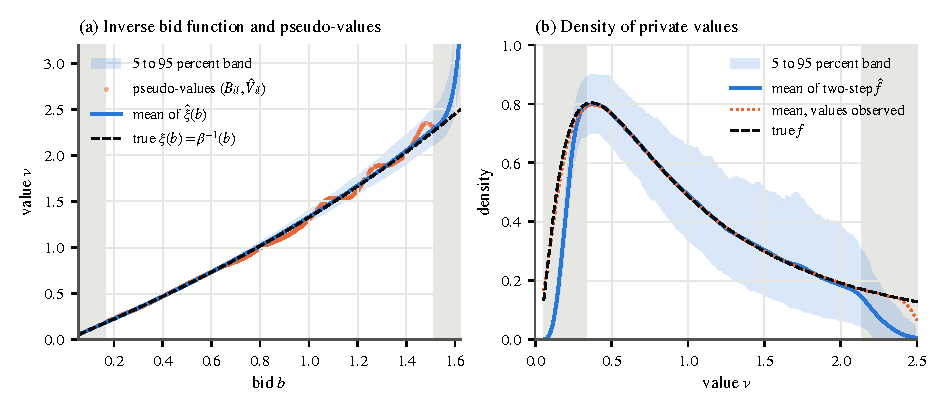
\includegraphics[width=\textwidth]{figures/appA/gpv.pdf}
\caption{The two-step estimator of \citet{GuerrePerrigneVuong2000} in their Monte Carlo design: 200
auctions with 5 bidders, values log-normal$(0,1)$ truncated to $[0.055,2.5]$, triweight kernels,
rule-of-thumb bandwidths, 1,000 replications. (a) True inverse bid function, mean and pointwise
5 to 95 percent band of $\hat\xi(b)$, and the pseudo-values of the first replication. The shaded bids are
trimmed on average (within $h_g$ of the extreme bids). (b) True value density, mean and pointwise
5 to 95 percent band of the two-step estimate, and the mean of the infeasible estimate from true values.
The shaded regions lie outside GPV's interior region (their footnote~9). Seed 20261022, script
\texttt{gpv\_mc.py}. Design follows Guerre, Perrigne and Vuong (2000), Section 2.4.}
\label{fig:A-gpv}
\end{figure}

The comparison with the infeasible estimator quantifies the price of inversion. On the interior region
the mean integrated squared error of the two-step estimate is 0.0170, against 0.0035 when values are
observed, a ratio of 4.9. The band in panel (b) is correspondingly wide, especially to the right of the
mode, where the bid density is low and its estimation error is amplified by \eqref{eq:A-gpv-xi}. Near
the lower end the two-step estimate collapses toward zero. Its mean at $v=0.055$ is 0.0003, against a
true density of 0.132. This is the joint effect of trimming and boundary bias, and it is why GPV report
results only on the interior region.

\section{Nonparametric regression, deconvolution and bounds}\label{sec:A-npreg}

This section estimates conditional means without functional form, combines nonparametric and
parametric components, separates a common factor from idiosyncratic noise, and draws inferences when
the data identify only a set. The tools build on \cref{sec:A-kde}. Throughout, $(y_i,x_i)$ are i.i.d.,
$m(x)=\E[y_i\mid x_i=x]$ is the regression function, $\sigma^2(x)=\Var(y_i\mid x_i=x)$, and $f$ is the
density of the scalar regressor $x_i$ unless stated otherwise.

\subsection{The Nadaraya-Watson estimator}\label{sec:A-nw}

The regression function is $m(x)=\frac{\int yf(x,y)\,\dd y}{f(x)}$. Replacing the joint density by the
product kernel estimate $\hat f(x,y)=\frac{1}{n}\sum_i\mathcal{K}_h(x-x_i)\mathcal{K}_h(y-y_i)$ and using
$\int y\,\mathcal{K}_h(y-y_i)\,\dd y=y_i$ for a symmetric kernel gives the \emph{Nadaraya-Watson
estimator} \citep{Nadaraya1964,Watson1964}:
\begin{equation}\label{eq:A-nw}
\hat m_h(x)=\frac{\sum_{i=1}^{n}\mathcal{K}_h(x-x_i)\,y_i}{\sum_{i=1}^{n}\mathcal{K}_h(x-x_i)} .
\end{equation}
It is a weighted average of the outcomes, with weights that decline with distance from $x$. It also
solves $\min_a\sum_i\mathcal{K}_h(x-x_i)(y_i-a)^2$, so it is a \emph{local constant} least squares fit.

\begin{proposition}[Bias and variance of Nadaraya-Watson]\label{prop:A-nw}
Let $x$ be an interior point with $f(x)>0$. Let $f$ be continuously differentiable and $m$ twice
continuously differentiable near $x$, let $\sigma^2$ be continuous, and let $h\to0$ and $nh\to\infty$.
Then
\begin{equation}\label{eq:A-nw-bias-var}
\E[\hat m_h(x)]-m(x)\approx h^2\mu_2\left(\frac{m''(x)}{2}+\frac{m'(x)f'(x)}{f(x)}\right),\qquad
\Var(\hat m_h(x))\approx\frac{\sigma^2(x)\kappa_2}{nhf(x)},
\end{equation}
where $\approx$ means equality of the leading terms.
\end{proposition}

\begin{proof}[Derivation]
Write $\hat m_h(x)-m(x)=\frac{\hat A(x)}{\hat f(x)}$ with
$\hat A(x)=\frac{1}{n}\sum_i\mathcal{K}_h(x-x_i)(y_i-m(x))$ and $\hat f(x)=\frac{1}{n}\sum_i\mathcal{K}_h(x-x_i)$.
Since $\hat f(x)\xrightarrow{p}f(x)$, the leading terms of the bias and variance are those of
$\frac{\hat A(x)}{f(x)}$.

\emph{Bias.} Using $\E[y_i\mid x_i]=m(x_i)$ and substituting $x_i=x-hu$,
\begin{equation*}
\E[\hat A(x)]=\int\mathcal{K}(u)\,\{m(x-hu)-m(x)\}\,f(x-hu)\,\dd u .
\end{equation*}
Expand $m(x-hu)-m(x)=-hum'(x)+\frac{h^2u^2}{2}m''(x)+o(h^2)$ and $f(x-hu)=f(x)-huf'(x)+o(h)$. The product
is $-hum'f+h^2u^2(m'f'+\frac{1}{2}m''f)+o(h^2)$. The term linear in $u$ integrates to zero, so
$\E[\hat A(x)]=h^2\mu_2(m'(x)f'(x)+\frac{1}{2}m''(x)f(x))+o(h^2)$. Dividing by $f(x)$ gives the bias.

\emph{Variance.} The leading term is
$\frac{1}{n}\E[\mathcal{K}_h(x-x_i)^2(y_i-m(x))^2]=\frac{1}{nh}\int\mathcal{K}(u)^2\{\sigma^2(x-hu)+(m(x-hu)-m(x))^2\}f(x-hu)\,\dd u$,
which equals $\frac{\kappa_2\sigma^2(x)f(x)}{nh}$ to first order. Dividing by $f(x)^2$ gives the variance.
\end{proof}

The bias has two parts. The curvature term $\frac{1}{2}m''$ is shared with every local smoother. The
\emph{design bias} $\frac{m'f'}{f}$ arises because, where the regressor density slopes, more
observations sit on one side of $x$ than on the other. The local average then leans toward the side
with more data, and the slope of $m$ converts the imbalance into bias.

At a boundary the problem is worse. Let the design have support $[0,\infty)$ with $f(0)>0$ and
evaluate at $x=0$. Only $u\le0$ contributes, so
$\E[\hat A(0)]\approx-hm'(0)f(0)\int_{-\infty}^{0}u\mathcal{K}(u)\,\dd u=hm'(0)f(0)\int_0^\infty u\mathcal{K}(u)\,\dd u$,
while $\hat f(0)\to\frac{1}{2}f(0)$. The bias is
\begin{equation}\label{eq:A-nw-boundary}
\E[\hat m_h(0)]-m(0)\approx2h\,m'(0)\int_0^\infty u\mathcal{K}(u)\,\dd u=\frac{3}{8}\,h\,m'(0)
\quad\text{(Epanechnikov kernel)},
\end{equation}
which is of order $h$ against $h^2$ in the interior. The Epanechnikov value
$\int_0^\infty u\mathcal{K}(u)\,\dd u=\frac{3}{16}$ is taken from \cref{tab:A-kernels}. For the four compact kernels of
that table the integral runs over $[0,1]$.

\subsection{Local polynomial regression}\label{sec:A-loclin}

The local constant fit ignores the slope of $m$. Fitting a line locally removes the design bias and the
first-order boundary bias. The \emph{local linear estimator} solves
\begin{equation}\label{eq:A-loclin}
(\hat a,\hat b)=\argmin_{a,b}\sum_{i=1}^{n}\mathcal{K}_h(x_i-x)\,\{y_i-a-b(x_i-x)\}^2,\qquad
\hat m_{\mathrm{LL}}(x)=\hat a .
\end{equation}
Let $S_j=\sum_i\mathcal{K}_h(x_i-x)(x_i-x)^j$. Solving the two normal equations gives
\begin{equation}\label{eq:A-loclin-weights}
\hat m_{\mathrm{LL}}(x)=\frac{\sum_iw_iy_i}{\sum_iw_i},\qquad w_i=\mathcal{K}_h(x_i-x)\{S_2-(x_i-x)S_1\}.
\end{equation}
The weights satisfy $\sum_iw_i(x_i-x)=S_1S_2-S_2S_1=0$. The estimator therefore reproduces any linear
function exactly, whatever the design.

\begin{proposition}[Local linear regression]\label{prop:A-loclin}
Let $\mathcal{K}$ vanish outside $[-1,1]$ and let $m$ be twice continuously differentiable. Conditional
on the regressors, and whenever $\sum_iw_i\ne0$,
\begin{equation*}
\E[\hat m_{\mathrm{LL}}(x)\mid x_1,\dots,x_n]-m(x)=\frac{\sum_iw_i\,\frac{1}{2}m''(\tilde x_i)(x_i-x)^2}{\sum_iw_i},
\end{equation*}
with $\tilde x_i$ between $x$ and $x_i$. Under the conditions of \cref{prop:A-nw}, the conditional bias at an
interior point is $\frac{h^2}{2}\mu_2m''(x)+o_p(h^2)$, free of the design term. At boundary points it remains of order
$h^2$. The interior variance is the Nadaraya-Watson variance $\frac{\sigma^2(x)\kappa_2}{nhf(x)}$
\citep{FanGijbels1996}.
\end{proposition}

\begin{proof}[Derivation]
Write $y_i=m(x)+m'(x)(x_i-x)+r_i+e_i$, where $r_i=\frac{1}{2}m''(\tilde x_i)(x_i-x)^2$ and
$\E[e_i\mid x_i]=0$. Substituting into \eqref{eq:A-loclin-weights}, the constant returns $m(x)$ and the
linear term vanishes because $\sum_iw_i(x_i-x)=0$. What remains is
$\frac{\sum_iw_i(r_i+e_i)}{\sum_iw_i}$, whose conditional mean is the displayed bias. Only observations
with $|x_i-x|\le h$ receive weight, so $|r_i|\le\frac{1}{2}h^2\sup|m''|$ wherever $x$ lies, and the bias
is $O_p(h^2)$ as long as $\frac{\sum_i|w_i|}{|\sum_iw_i|}$ stays bounded. That ratio is bounded at the
boundary too, because $S_0S_2-S_1^2>0$ when the window contains data on a set of positive length. In the
interior, $\frac{S_0}{n}\xrightarrow{p}f(x)$, $\E[\frac{S_1}{n}]=h^2\mu_2f'(x)+o(h^2)$ and $\Var(\frac{S_1}{n})=O(\frac{h}{n})$.
Hence $\frac{S_1}{S_0}=O_p(h^2+\sqrt{\frac{h}{n}})=o_p(h)$, because $\sqrt{\frac{h}{n}}=\frac{h}{\sqrt{nh}}$ and
$nh\to\infty$. The same calculation gives $\frac{S_2}{S_0}=h^2\mu_2+o_p(h^2)$. For $|x_i-x|\le h$ the
correction $\frac{(x_i-x)S_1}{S_2}$ in the weights is then $o_p(1)$. The weights therefore behave like
$\mathcal{K}_h(x_i-x)$ to first order, and the bias becomes $\frac{h^2}{2}\mu_2m''(x)$. The variance
argument is that of \cref{prop:A-nw}.
\end{proof}

Fitting a polynomial of degree $p$ in place of a line gives the \emph{local polynomial} estimator. The
coefficient on $(x_i-x)^k$ estimates $\frac{m^{(k)}(x)}{k!}$, so the slope $\hat b$ in
\eqref{eq:A-loclin} is a natural estimator of $m'(x)$. Odd degrees are preferred because they adapt
automatically to the boundary \citep{FanGijbels1996}.

\Cref{fig:A-npreg} compares the two estimators with the same Epanechnikov kernel and bandwidth $h=0.10$.
The design density is $\frac{2}{3}(1+x)$ on $[0,1]$ and the regression function is $m(x)=2e^{-5x}+0.5x$,
which is steep at the left boundary, with $m'(0)=-9.5$. With $n=400$, noise standard deviation 0.25 and
1,000 samples, the bias of Nadaraya-Watson at $x=0$ is $-0.316$. The approximation
\eqref{eq:A-nw-boundary} gives $-0.356$, and the difference reflects the large curvature of $m$ near
zero. The local linear bias at $x=0$ is $-0.028$. Its standard deviation there is larger, 0.105 against
0.064, because a line fitted at the edge extrapolates. In the interior both estimators share the
curvature bias, which reaches 0.031 for local linear near $x=0.1$, where $m''=50e^{-0.5}\approx30$.
Local fitting removes the design term and leaves the curvature term.

\begin{figure}[htbp]
\centering
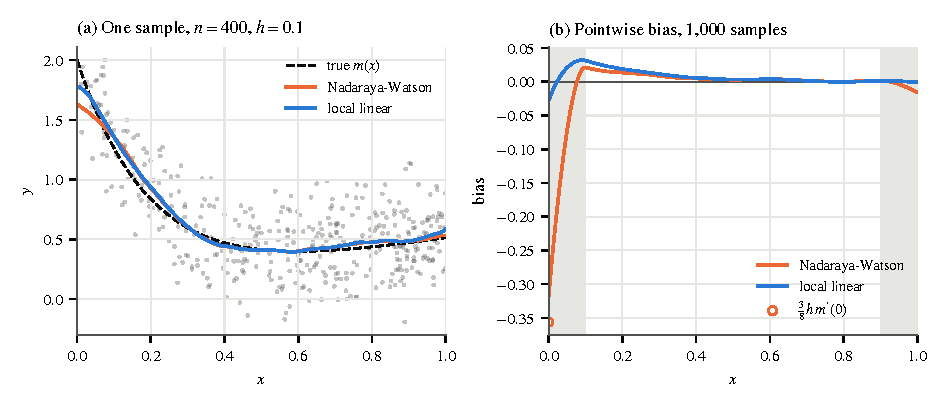
\includegraphics[width=\textwidth]{figures/appA/npreg.pdf}
\caption{Nadaraya-Watson and local linear regression with the same Epanechnikov kernel and bandwidth
$h=0.10$. The regressor has density $\frac{2}{3}(1+x)$ on $[0,1]$, $m(x)=2e^{-5x}+0.5x$, and the noise is
$N(0,0.25^2)$, $n=400$. (a) One sample. (b) Pointwise bias over 1,000 samples. The shaded
strips are within one bandwidth of the boundary, and the marker shows the boundary approximation
$\frac{3}{8}hm'(0)$ of \eqref{eq:A-nw-boundary}. Seed 20261022, script \texttt{npreg\_demo.py}.}
\label{fig:A-npreg}
\end{figure}

\casehead{Applications in the book}
Three applications use local regression. First, \citet{HausmanNewey1995} estimate demand $q(p,y)$
nonparametrically, as a function of price and income, and carry out the exact welfare analysis with it
\citep[fn.~6]{Hausman1997}. The exact analysis solves the differential equation of \citet{Hausman1981}. For a price change from
$p^0$ to $p^1$, let $S(p)=e(p,u^0)-y$ be the extra income needed to keep utility at its initial level.
Shephard's lemma and duality give
\begin{equation}\label{eq:A-hausman-ode}
\frac{\dd S(p)}{\dd p}=q\bigl(p,\,y+S(p)\bigr),\qquad S(p^0)=0,
\end{equation}
and the compensating variation is $S(p^1)$ (\cref{app:math}). \citet{Hausman1997} solves the same
differential equation for a parametric demand system for a new breakfast cereal. His exact welfare estimates and
their standard errors use the method of \citet{HausmanNewey1995} (his fn.~24, \cref{ch:newgoods}). Second, \citet[eq.~(18)]{BajariBenkard2005} recover
each product's unobserved characteristic as a conditional quantile. Normalizing $\xi$ to be uniform on
$[0,1]$ and independent of $x$, with price increasing in $\xi$, they set
$\hat\xi_{jt}=\hat F_{p_t\mid x=x_j}(p_{jt})$. In their application a local linear kernel estimator
\citep{FanGijbels1996} with a normal kernel worked best \citep[Sections~5.1 and~6]{BajariBenkard2005}.
Derivatives of the estimated hedonic price function then recover consumers' marginal valuations from
their first-order conditions (\cref{ch:discrete}). Third, conditional bid distributions given covariates
can be estimated by local linear smoothing of indicator outcomes $\indic\{B_{il}\le b\}$, which avoids
the boundary problems of \cref{sec:A-kde-boundary} in the covariate dimension.

\subsection{Series and sieve estimators}\label{sec:A-series}

A \emph{series estimator} approximates $m$ by a linear combination of $K_n$ known basis functions
$\psi(x)=(\psi_1(x),\dots,\psi_{K_n}(x))^\top$, such as powers of $x$ or regression splines. A regression
spline of degree $r$ is a polynomial of degree $r$ between consecutive points called knots, with $r-1$ continuous
derivatives at each knot. B-splines are a convenient basis for this space. The series estimator fits the
coefficients by least squares,
\begin{equation}\label{eq:A-series}
\hat m(x)=\psi(x)^\top\hat\gamma,\qquad \hat\gamma=(\Psi^\top\Psi)^{-1}\Psi^\top y .
\end{equation}
Here $\Psi$ is the $n\times K_n$ matrix with rows $\psi(x_i)^\top$. The number of terms plays the role of
the inverse bandwidth. Its variance cost has an exact expression. With homoskedastic errors of variance
$\sigma^2$, the fitted values are $P_\Psi y$ with $P_\Psi=\Psi(\Psi^\top\Psi)^{-1}\Psi^\top$, so
\begin{equation*}
\frac{1}{n}\sum_{i=1}^{n}\Var(\hat m(x_i)\mid\Psi)=\frac{\sigma^2}{n}\,\mathrm{tr}(P_\Psi)=\frac{\sigma^2K_n}{n}.
\end{equation*}
For a function with $R$ derivatives and a polynomial or spline basis in one dimension, the squared
approximation bias is of order $K_n^{-2R}$. Balancing the two gives $K_n\propto n^{\frac{1}{2R+1}}$ and the
same mean squared error rate $n^{-\frac{2R}{2R+1}}$ as a kernel estimator \citep{Newey1997}. In practice
$K_n$ is chosen by cross-validation or an information criterion.

Series estimators are global. A misbehaving term affects the fit everywhere, and high-order
polynomials are unstable at the boundary, which favors splines. In exchange, restrictions such as
additivity, $m(x)=m_1(x_1)+m_2(x_2)$, are easy to impose by choosing the basis, and the estimator is a
least squares regression whose inference is standard for fixed $K_n$. A \emph{sieve} is the general
version. It is a sequence of increasingly rich approximating function classes, and the estimator uses a richer
class as $n$ grows \citep{Chen2007}. Three uses appear in
the book. Approximations to optimal instruments use series in the instruments (\cref{sec:A-optimal-iv}).
The marginal cost of an airline segment in \citet{BerryCarnallSpiller1996} is a cubic polynomial in leg
distance and leg density, with two congestion shifters (WP Table~5, \cref{sec:09-bcs-supply}). It is a
fixed low-order series. And
\citet[footnote~20]{AtheyHaile2007} point to sieve estimation as a practical alternative to kernels
in auctions with observed heterogeneity.

\subsection{The partially linear model}\label{sec:A-plm}

Often only a few parameters are of interest, while a control variable enters in an unknown way. The
\emph{partially linear model} is
\begin{equation}\label{eq:A-plm}
y_i=x_i^\top\beta+m(w_i)+e_i,\qquad \E[e_i\mid x_i,w_i]=0,
\end{equation}
with $m$ unknown. Taking expectations conditional on $w_i$ gives
$\E[y_i\mid w_i]=\E[x_i\mid w_i]^\top\beta+m(w_i)$. Subtracting this from \eqref{eq:A-plm} eliminates
$m$:
\begin{equation}\label{eq:A-robinson}
\tilde y_i=\tilde x_i^\top\beta+e_i,\qquad \tilde y_i=y_i-\E[y_i\mid w_i],\quad \tilde x_i=x_i-\E[x_i\mid w_i].
\end{equation}
\citet{Robinson1988} estimates the two conditional means nonparametrically and regresses the
residual of $y$ on the residual of $x$ by least squares. This is the \emph{double-residual estimator}.

\begin{proposition}[Robinson's estimator]\label{prop:A-robinson}
Suppose $\E[\tilde x_i\tilde x_i^\top]$ is positive definite, so no linear combination of $x_i$ is a
function of $w_i$ alone. Suppose the first-step estimators of $\E[y\mid w]$ and $\E[x\mid w]$ converge
in mean square faster than $n^{-\frac{1}{4}}$, with trimming and kernel order as in
\citet{Robinson1988}. Then
\begin{equation*}
\sqrt n(\hat\beta-\beta)\xrightarrow{d}N\!\left(0,\ \E[\tilde x\tilde x^\top]^{-1}\E[e^2\tilde x\tilde x^\top]\E[\tilde x\tilde x^\top]^{-1}\right),
\end{equation*}
the distribution of the infeasible regression with known conditional means.
\end{proposition}

\begin{proof}[Why the first step does not matter]
The estimator solves the sample analogue of the moment
$\E[(\tilde y-\tilde x^\top\beta)\tilde x]=0$. Perturb the conditional means by functions $\delta_y(w)$
and $\delta_x(w)$, so the moment becomes
$M(\delta)=\E[\{\tilde y-\delta_y(w)-(\tilde x-\delta_x(w))^\top\beta\}\{\tilde x-\delta_x(w)\}]$. Its
derivative at $\delta=0$ in the direction $\delta_y$ is $-\E[\delta_y(w)\tilde x]$, which is zero because
$\E[\tilde x\mid w]=0$. In the direction $\delta_x$ the derivative is
$\E[\tilde x\,\delta_x(w)^\top]\beta-\E[e\,\delta_x(w)]$, and both terms vanish by
$\E[\tilde x\mid w]=0$ and $\E[e\mid w]=0$. First-step errors therefore enter only through products of
two errors, of order $\|\hat\delta\|^2$. If $\|\hat\delta\|=o_p(n^{-\frac{1}{4}})$, these products are
$o_p(n^{-\frac{1}{2}})$, and the infeasible limit applies.
\end{proof}

The estimator is the nonparametric analogue of the Frisch-Waugh-Lovell theorem (\cref{thm:A-fwl}). If
$m(w)=w^\top\gamma$, partialling out $w$ by linear projection and regressing residual on residual
reproduces the coefficient on $x$ in the long regression. Robinson replaces the linear projection by
the conditional expectation, which partials out every function of $w$. The insensitivity to the first
step derived in the proof is the property now called \emph{Neyman orthogonality}.

A simulation in \texttt{npreg\_demo.py} shows what is at stake. Let $w$ be uniform on $[0,1]$,
$x=\sin(2\pi w)+v$ and $y=x+2\sin(2\pi w)+e$, with $v$ and $e$ standard normal, $n=500$ and 1,000 samples.
Least squares of $y$ on a constant, $x$ and $w$ controls for $w$ linearly. Its mean estimate is 1.327
against $\beta=1$, and its nominal 95 percent interval never covers the truth. Robinson's estimator with
local linear first steps ($h=0.08$) has mean 0.999 and standard deviation 0.045, equal to the infeasible
value $\frac{1}{\sqrt{500}}\approx0.045$. Its interval covers in 94.1 percent of samples.

\subsection{Deconvolution}\label{sec:A-deconv}

Suppose two noisy measurements share a common component,
\begin{equation}\label{eq:A-meas}
Y_1=U+\epsilon_1,\qquad Y_2=U+\epsilon_2,
\end{equation}
with $U$, $\epsilon_1$ and $\epsilon_2$ mutually independent. In auctions, $U$ is the log of a factor that
scales all bids in an auction, known to the bidders and unobserved by us. The term $\epsilon_j$ is the log of the
bid that bidder $j$ would make if the factor were one. The goal is the distribution of each
component from the joint distribution of $(Y_1,Y_2)$.

Second moments show why two measurements help. Independence gives $\Cov(Y_1,Y_2)=\Var(U)$, so
$\Var(\epsilon_j)=\Var(Y_j)-\Cov(Y_1,Y_2)$, and the normalization $\E[\epsilon_1]=0$ gives
$\E[U]=\E[Y_1]$. Variation across auctions identifies the spread of the common factor, and variation
within auctions identifies the spread of the idiosyncratic parts. A theorem of \citet{Kotlarski1966}
extends this from second moments to whole distributions. Let
$\varphi_U(t)=\E[e^{\mathrm{i}tU}]$ denote a characteristic function, where $\mathrm{i}$ is the
imaginary unit, and let $\varphi_{Y_1Y_2}(t_1,t_2)=\E[e^{\mathrm{i}t_1Y_1+\mathrm{i}t_2Y_2}]$.

\begin{lemma}[Kotlarski]\label{lem:A-kotlarski}
In \eqref{eq:A-meas}, let $U$, $\epsilon_1$, $\epsilon_2$ be mutually independent with finite first
moments and $\E[\epsilon_1]=0$, and let $\varphi_U$ and $\varphi_{\epsilon_2}$ never vanish. Then for every
real $t$,
\begin{equation}\label{eq:A-kotlarski}
\varphi_U(t)=\exp\left(\int_0^t\frac{\E\left[\mathrm{i}Y_1e^{\mathrm{i}sY_2}\right]}{\E\left[e^{\mathrm{i}sY_2}\right]}\,\dd s\right),\qquad
\varphi_{\epsilon_1}(t)=\frac{\varphi_{Y_1Y_2}(t,0)}{\varphi_U(t)},\qquad
\varphi_{\epsilon_2}(t)=\frac{\varphi_{Y_1Y_2}(0,t)}{\varphi_U(t)} .
\end{equation}
The joint distribution of $(Y_1,Y_2)$ therefore determines the distributions of $U$, $\epsilon_1$ and
$\epsilon_2$.
\end{lemma}

\begin{proof}
Independence factors the joint characteristic function:
\begin{equation*}
\varphi_{Y_1Y_2}(t_1,t_2)=\E\left[e^{\mathrm{i}(t_1+t_2)U}e^{\mathrm{i}t_1\epsilon_1}e^{\mathrm{i}t_2\epsilon_2}\right]
=\varphi_U(t_1+t_2)\,\varphi_{\epsilon_1}(t_1)\,\varphi_{\epsilon_2}(t_2).
\end{equation*}
Finite first moments make the characteristic functions continuously differentiable, with
$\varphi_X'(0)=\mathrm{i}\E[X]$. Differentiating in $t_1$ and setting $t_1=0$, with $\varphi_{\epsilon_1}(0)=1$
and $\varphi_{\epsilon_1}'(0)=\mathrm{i}\E[\epsilon_1]=0$,
\begin{equation*}
\frac{\partial\varphi_{Y_1Y_2}}{\partial t_1}(0,s)=\varphi_U'(s)\,\varphi_{\epsilon_2}(s).
\end{equation*}
The left side equals $\E[\mathrm{i}Y_1e^{\mathrm{i}sY_2}]$, and $\varphi_{Y_1Y_2}(0,s)=\E[e^{\mathrm{i}sY_2}]=\varphi_U(s)\varphi_{\epsilon_2}(s)\ne0$.
Dividing, $\varphi_{\epsilon_2}(s)$ cancels:
\begin{equation*}
\frac{\E[\mathrm{i}Y_1e^{\mathrm{i}sY_2}]}{\E[e^{\mathrm{i}sY_2}]}=\frac{\varphi_U'(s)}{\varphi_U(s)}=\frac{\dd}{\dd s}\log\varphi_U(s),
\end{equation*}
where $\log$ is the continuous branch with $\log\varphi_U(0)=0$, which exists because $\varphi_U$ is
continuous and never zero. Integrating from 0 to $t$ and exponentiating gives the first formula. Setting
$t_2=0$, and then $t_1=0$, in the factorization gives $\varphi_{Y_1Y_2}(t,0)=\varphi_U(t)\varphi_{\epsilon_1}(t)$ and
$\varphi_{Y_1Y_2}(0,t)=\varphi_U(t)\varphi_{\epsilon_2}(t)$, and division gives the other two. A characteristic
function determines its distribution.
\end{proof}

Each assumption has a role. Independence delivers the factorization. The nonvanishing condition allows
the divisions and the logarithm. The zero mean of $\epsilon_1$ is a location normalization, since a
constant could otherwise move freely between $U$ and the $\epsilon$'s. The lemma identifies
distributions only. The realization of $U$ in a given auction is not identified. \Cref{ch:collusion-evidence} states
the same result for Asker's application.

The nonvanishing condition deserves care. \citet[Lemma~1]{Krasnokutskaya2011} argues that a variable
with bounded support has a characteristic function that extends to an entire function, so its zeros are
isolated. Isolated zeros can still occur, as the uniform distribution shows, since its characteristic
function $\frac{\sin t}{t}$ vanishes at multiples of $\pi$. \citet{EvdokimovWhite2012} show that
identification survives some violations of the condition under additional restrictions.

\casehead{The estimator}
\citet{LiVuong1998} replace each characteristic function by its sample analogue. With $n$ independent
pairs $(Y_{1k},Y_{2k})$,
\begin{equation}\label{eq:A-lv}
\hat\varphi_U(t)=\exp\left(\int_0^t\frac{\frac{1}{n}\sum_k\mathrm{i}Y_{1k}e^{\mathrm{i}sY_{2k}}}{\frac{1}{n}\sum_ke^{\mathrm{i}sY_{2k}}}\,\dd s\right),\qquad
\hat f_U(u)=\frac{1}{2\pi}\int_{-T}^{T}d_T(t)\,e^{-\mathrm{i}tu}\,\hat\varphi_U(t)\,\dd t ,
\end{equation}
and analogously for $\epsilon_1$ and $\epsilon_2$. The density is recovered by the inverse Fourier
transform, truncated at $\pm T$ and multiplied by a \emph{damping factor} $d_T$ that downweights high
frequencies, such as $d_T(t)=\max\{1-\frac{|t|}{T},0\}$ \citep{DiggleHall1993}. Since
$\hat\varphi_U(-t)$ is the complex conjugate of $\hat\varphi_U(t)$, the estimate is real and equals
$\frac{1}{\pi}\int_0^Td_T(t)\,\mathrm{Re}\{e^{-\mathrm{i}tu}\hat\varphi_U(t)\}\,\dd t$. The truncation
point $T$ is the smoothing parameter, playing the role of an inverse bandwidth.

Deconvolution converges slowly. The empirical characteristic function has error of order
$n^{-\frac{1}{2}}$ at each frequency, but the formulas divide by quantities that decay at high
frequencies. The ratio in \eqref{eq:A-lv} divides by $\varphi_U(s)\varphi_{\epsilon_2}(s)$, and the formula
for $\varphi_{\epsilon_1}$ divides by $\varphi_U$. The achievable rate depends on how fast the characteristic
functions decay. It is polynomial in $n$ for \emph{ordinary smooth} distributions, whose characteristic
functions decay like $|t|^{-\beta}$, and only logarithmic for \emph{supersmooth} ones such as the normal
\citep{Fan1991}. \citet{LiVuong1998} establish uniform consistency under conditions of this kind.
Krasnokutskaya's consistency result assumes ordinary smooth components with $\beta>1$
\citep[Proposition~5]{Krasnokutskaya2011}.

\Cref{fig:A-deconv} implements \eqref{eq:A-lv} with $U$ distributed Gamma with shape 4 and scale 0.25
(mean 1, standard deviation 0.5), $\epsilon_j\sim N(0,0.4^2)$, $n=1{,}000$ pairs and 200 samples. With
$T=8$ the median integrated squared error of $\hat f_U$ is 0.035. A kernel density estimate of $Y_1$
ignores the noise and has mean integrated squared error 0.058. Raising $T$ to 10 lowers the median
error to 0.029 but makes the estimator unstable, with a mean integrated squared error of 2.44 driven by
a few samples. Too large a $T$ divides by empirical characteristic functions that are pure noise.

\begin{figure}[htbp]
\centering
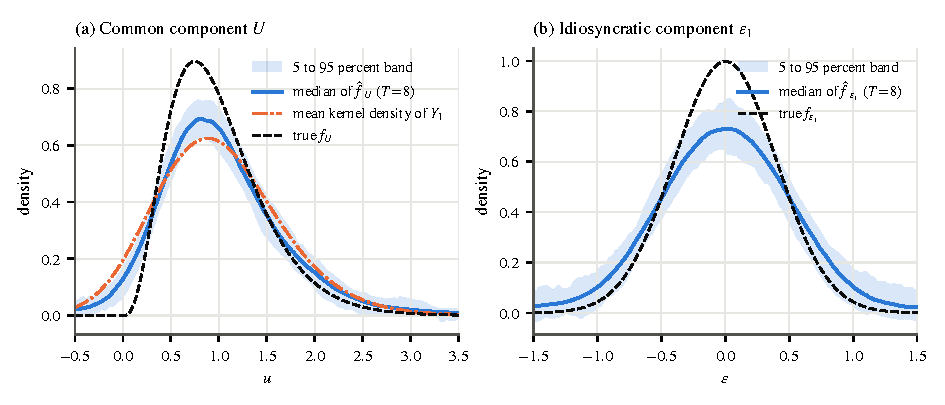
\includegraphics[width=\textwidth]{figures/appA/deconv.pdf}
\caption{Kotlarski deconvolution with the estimator of \citet{LiVuong1998}. $Y_j=U+\epsilon_j$ with
$U\sim\mathrm{Gamma}(4,0.25)$ and $\epsilon_j\sim N(0,0.4^2)$, $n=1{,}000$ pairs, smoothing parameter
$T=8$, damping factor $1-\frac{|t|}{T}$, 200 samples. (a) True density of $U$, pointwise median
and 5 to 95 percent band of $\hat f_U$, and the mean rule-of-thumb kernel density estimate of $Y_1$.
(b) The same for $\epsilon_1$. Seed 20261022, script \texttt{npreg\_demo.py}.}
\label{fig:A-deconv}
\end{figure}

\casehead{Krasnokutskaya's procurement auctions}
\citet{Krasnokutskaya2011} applies the lemma to first-price procurement auctions. A bidder's cost is
the product of a project-level component $Y$, common knowledge among bidders and unobserved by us, and an
individual component. The equilibrium bid inherits the product structure, $B_{ij}=y_ja_{ij}$, where
$a_{ij}$ is the bid at $y=1$. For two bidders in the same auction, logs give
$\log B_{i_1}=\log Y+\log A_{i_1}$ and $\log B_{i_2}=\log Y+\log A_{i_2}$. Her equation~(3) is
\eqref{eq:A-kotlarski} for these variables.\footnote{Its equation~(3) prints a logarithm where the
exponential of \eqref{eq:A-kotlarski} belongs. The estimator in its appendix uses the exponential.} The
location is fixed by $\E[\log A_1]=0$. Her estimator averages the empirical characteristic function over
all pairs of bidders of the relevant types. It scales bids into $[0,2]$ to reduce estimation error in the
characteristic function. It uses the damping factor $1-\frac{|t|}{T}$ and chooses $T$ to match the means
and variances of $\log Y$ and $\log A$ implied by the bids, which selects $T=50$ in her application. The
moment conditions behind the choice of $T$ are the second-moment identities above. With identically
distributed individual components, $\Var(\log A)=\frac{1}{2}\E[(\log B_1-\log B_2)^2]$ and
$\Var(\log Y)=\Var(\log B)-\Var(\log A)$ \citep[Section~4.3]{Krasnokutskaya2011}. In a second step she
draws pseudo-bids from the estimated density of the individual component by rejection sampling. She
converts them to pseudo-costs through the asymmetric first-order condition. The densities in this step
use a triweight kernel and the bandwidth $2.978\times1.06\,\hat\sigma L^{-\frac{1}{6}}$, where
$\hat\sigma$ is the standard deviation of the log of one plus the bids. Confidence intervals come from
the bootstrap. Independence also generates testable restrictions. The characteristic functions
recovered from different pairs and triples of bidders must agree. A degenerate $\log Y$ gives the
independent private values model, which can be tested within the same framework (her conditions W1 to
W7). In Michigan highway procurement auctions she attributes about 75 percent of the variation in
bidders' costs to factors known to all bidders. Only 25 percent comes from private information
(abstract of the working paper). \citet[p.~103]{HortacsuPerrigne2021} report the published estimate as 34 percent
of the bid variation from private information. That figure refers to bids, while the working-paper figure refers to
costs. \Cref{ch:auction-empirics} discusses the application.

\casehead{Asker's knockout bids}
\citet{Asker2010} applies the same estimator to pairs of normalized knockout bids in a stamp-dealer ring,
$\ln\hat b_{1k}=\ln(\varepsilon_k)+\ln\beta(v_{1k})$ and $\ln\hat b_{2k}=\ln(\varepsilon_k)+\ln\beta(v_{2k})$
(his eq.~(4)). In his notation the common component of lot $k$ is $\ln(\varepsilon_k)$, which plays the
role of $U$ in \eqref{eq:A-meas}. He imposes $\E[\ln\beta(v_1)]=0$ and independence (his Assumption~U).
The target-auction price supplies a third measurement of the common component. He averages the estimated characteristic
functions from the two kinds of pairs, weighting by the number of observations of each, as
\citet{LiVuong1998} suggest. His damping factor is $\max\{1-\frac{|t|}{\sqrt2T_n},0\}$. The smoothing
parameter is $T_n=50$ for the common component, whose estimate proved insensitive to it. For the strong
members, the weak members and the highest non-ring value, the values 12.0, 3.0 and 8.3 minimize a
criterion. The criterion matches naive damages and the ring's win probability and penalizes
non-monotone bid functions \citep[pp.~748--749]{Asker2010}. As with Krasnokutskaya, only distributions are identified, and
the GPV inversion is applied to draws from the estimated distributions (\cref{ch:collusion-evidence}).

\subsection{Estimation and inference under partial identification}\label{sec:A-partialid}

When the model and data restrict a parameter only to a set, the parameter is \emph{partially identified}
(\cref{def:A-identification}). A common form is a set of moment inequalities,
\begin{equation}\label{eq:A-mi}
\Theta_I=\{\theta\in\Theta:\ \E[m_j(W;\theta)]\ge0,\ j=1,\dots,J\},
\end{equation}
where $\Theta_I$ is the \emph{identified set}. Every point of $\Theta_I$ is consistent with the population
distribution of the data, and no point outside it is. Estimation targets the set, and inference can
target either the set or the true parameter inside it.

\casehead{Bounds in English auctions}
\citet{HaileTamer2003} drop the button-auction model of ascending auctions, in which bidders exit at
their values. They impose two behavioral assumptions. Bidders never bid more than their value, and
bidders never let an opponent win at a price they would have been willing to beat. Let $G_{k:n}$ be the
distribution of the $k$-th lowest bid in $n$-bidder auctions. Let $G^{\Delta}_{n:n}$ be the distribution
of the winning bid plus the minimum increment $\Delta$, and $\phi_{k:n}$ the map from $F$ to $F_{(k:n)}$
in \eqref{eq:A-orderstat}. The first assumption implies that the $k$-th lowest bid is at most the $k$-th
lowest value, so $G_{k:n}(v)\ge\phi_{k:n}(F(v))$. The second implies that the second-highest value is at
most the winning bid plus $\Delta$, so $\phi_{n-1:n}(F(v))\ge G^{\Delta}_{n:n}(v)$. Inverting the
increasing maps and combining all order statistics and all $n$ gives
\citep[Section~4.3.1, eqs.~(4.10)--(4.11)]{AtheyHaile2007}
\begin{equation}\label{eq:A-ht}
F^-(v)=\max_n\ \phi_{n-1:n}^{-1}\!\left(G^{\Delta}_{n:n}(v)\right)\ \le\ F(v)\ \le\
F^+(v)=\min_{n}\min_{1\le k\le n}\ \phi_{k:n}^{-1}\!\left(G_{k:n}(v)\right).
\end{equation}
\Cref{ch:auction-empirics} develops the bounds and their use for reserve prices.
\citet[pp.~493--499]{AradillasLopezGandhiQuint2013} derive bounds on expected profit, bidder surplus and
the optimal reserve price when symmetric private values have nonnegative dependence. They use only the transaction price and,
with values independent of the number of bidders, variation in that number across auctions.
\citet[footnote~37]{Asker2010}
discusses why he does not use the Haile-Tamer approach. Jump bidding was rare at the stamp auctions he
observed, and bid increments were small relative to bids.

\casehead{Plug-in estimation and the bias of extrema}
The natural estimator of \eqref{eq:A-ht} replaces each $G$ by an empirical distribution function. The
minimum and maximum then create a finite-sample bias. The minimum is concave, so by Jensen's inequality
$\E[\min_j\hat a_j]\le\min_j\E[\hat a_j]$. A worked case shows the size. Let $\hat a_1$ and $\hat a_2$ be
independent $N(a,\sigma^2)$, both unbiased for the same bound $a$. Since $\min(a_1,a_2)=\frac{a_1+a_2}{2}-\frac{|a_1-a_2|}{2}$
and $\hat a_1-\hat a_2\sim N(0,2\sigma^2)$ has mean absolute value $\frac{2\sigma}{\sqrt\pi}$,
\begin{equation*}
\E\left[\min(\hat a_1,\hat a_2)\right]=a-\frac{\sigma}{\sqrt\pi}.
\end{equation*}
The estimated upper bound is too low and the estimated lower bound too high, so the estimated set is too
narrow. The bias grows with the number of terms in the minimum. \citet{HaileTamer2003} define the
bounds in finite samples with smooth approximations to the max and min functions. In the words of
\citet[Section~4.3.1, p.~35]{AtheyHaile2007}, this ``amounts to using weighted averages instead of the max or min.''
For example, the softmax-weighted average
$\sum_j\hat a_j\frac{e^{\rho\hat a_j}}{\sum_ke^{\rho\hat a_k}}$ with $\rho<0$ is a smooth minimum of
this kind. It tends to $\min_j\hat a_j$ as $\rho\to-\infty$, and it lies above the minimum, which
offsets the downward bias. We use it only as an illustration, and it need not be the weighting that Haile
and Tamer choose.

The extrema also break standard inference. The functional $\min(a_1,a_2)$ is not differentiable where
$a_1=a_2$, so the delta method fails there, and the bootstrap can fail for the same reason
(\cref{prop:A-boot-max}).

\casehead{Set estimators and confidence regions}
Define the criterion $Q(\theta)=\sum_j(\min\{\E[m_j(W;\theta)],0\})^2$, which is zero exactly on
$\Theta_I$. Its sample analogue $Q_n$ is zero on the sample identified set, which may be empty or too
small. \citet{ChernozhukovHongTamer2007} estimate the set by $\hat\Theta_I=\{\theta:\ nQ_n(\theta)\le c_n\}$
with $c_n\to\infty$ and $\frac{c_n}{n}\to0$. The Hausdorff distance between sets $A$ and $B$ is
\begin{equation*}
d_H(A,B)=\max\Bigl\{\sup_{a\in A}\inf_{b\in B}\lVert a-b\rVert,\ \sup_{b\in B}\inf_{a\in A}\lVert a-b\rVert\Bigr\}.
\end{equation*}
It is the larger of two directed distances. Each is the largest distance from a point of one set to the nearest
point of the other. The estimator is consistent in this distance, so $d_H(\hat\Theta_I,\Theta_I)\to0$ in
probability. Confidence regions
for $\Theta_I$ invert tests of $Q(\theta)=0$, with cutoffs from subsampling or the bootstrap.

For an interval $[\theta_l,\theta_u]$ there is an important distinction. A region that covers the whole
set with probability $1-\alpha$ is larger than one that covers the true parameter with that probability.
\citet{ImbensManski2004} construct the second kind. With estimators $\hat\theta_l$ and $\hat\theta_u$,
standard errors $\frac{\hat\sigma_l}{\sqrt n}$ and $\frac{\hat\sigma_u}{\sqrt n}$, and estimated length
$\hat\Delta=\hat\theta_u-\hat\theta_l$, the interval is
\begin{equation}\label{eq:A-im}
\left[\hat\theta_l-c_n\frac{\hat\sigma_l}{\sqrt n},\ \hat\theta_u+c_n\frac{\hat\sigma_u}{\sqrt n}\right],\qquad
\Phi\!\left(c_n+\frac{\sqrt n\,\hat\Delta}{\max\{\hat\sigma_l,\hat\sigma_u\}}\right)-\Phi(-c_n)=1-\alpha .
\end{equation}
When the set is long relative to sampling error, the true parameter can be near at most one end point.
Only one tail then matters, and $c_n$ approaches the one-sided value 1.645 for $\alpha=0.05$. When the set
shrinks to a point, $c_n$ rises to the two-sided 1.96. A region for the whole set needs both end
points covered at once and uses a larger constant. \citet{Stoye2009} refines the argument for sets whose
length is near zero. \citet{Manski2003} and \citet{Tamer2010} survey the field.

\section{Difference in differences and panel event studies}\label{sec:A-did}

The last two sections of the appendix turn from estimators to research designs. Many questions in industrial
organization concern a discrete change in a market. Two firms merge, a rival
enters, a state raises a tax, or a patent is granted. A \emph{retrospective} (or ex post) evaluation measures
what the change did by comparing outcomes after it with outcomes before it. A \emph{prospective} (or ex ante)
evaluation predicts the effect before the change, with a model of demand, costs and conduct. This section
develops the research designs behind retrospectives. They compare units exposed to the change with units that
were not, before and after the change.

These designs are reduced form. They identify average effects of a change under assumptions about the outcomes
that units would have had without it, and they need no model of conduct. The book uses them for merger
retrospectives (\cref{sec:11-retro}), tax pass-through (\cref{sec:03-sumner}), entry
(\cref{sec:09-wc-did}) and patents (\cref{sec:05-dgg}). We build on the potential-outcomes notation of
\cref{sec:A-potential}. Throughout this section $i$ indexes units (products, markets, states, hospitals) and
$t$ indexes periods, and $\tau_t$ denotes a period fixed effect. In \cref{sec:A-eventstudy} the symbol $\tau$ will
index trading days instead.

\subsection{The two-by-two design}\label{sec:A-did-2x2}

We start with two groups and two periods. Units $i=1,\dots,n$ are observed in periods $t\in\{0,1\}$. The
indicator $\mathit{Treat}_i$ equals one for units in the \emph{treated group}, which is exposed to the change
between the two periods. The other units form the \emph{control group}. Let $\mathit{Post}_t=\indic\{t=1\}$ and
let $d_{it}=\mathit{Treat}_i\,\mathit{Post}_t$ be the treatment indicator. Each unit has two potential outcomes in
each period, $y_{it}(1)$ with the treatment and $y_{it}(0)$ without it. We observe
\begin{equation*}
y_{it}=y_{it}(0)+d_{it}\big[y_{it}(1)-y_{it}(0)\big].
\end{equation*}

\begin{definition}[Average effect of the treatment on the treated]\label{def:A-att}
The \emph{average treatment effect on the treated} in the post period, the panel version of the ATT of
\cref{sec:A-potential}, is
\begin{equation*}
\mathrm{ATT}=\E\big[y_{i1}(1)-y_{i1}(0)\mid \mathit{Treat}_i=1\big].
\end{equation*}
\end{definition}

Two naive comparisons fail. The cross-sectional comparison of treated and control units in period 1 adds a
selection term, the difference in untreated outcomes between the groups (\cref{prop:A-selection}). The
before-after comparison within the treated group adds the change that the treated units would have experienced
anyway:
\begin{equation*}
\E\big[y_{i1}-y_{i0}\mid\mathit{Treat}_i=1\big]=\mathrm{ATT}+\E\big[y_{i1}(0)-y_{i0}(0)\mid\mathit{Treat}_i=1\big],
\end{equation*}
provided that period-0 outcomes are untreated. A rise in input costs at the time of a merger, for example, is
attributed to the merger. The \emph{difference-in-differences} (DiD) estimator removes this change with the change
in the control group. Let $\bar y_{T,t}$ and $\bar y_{C,t}$ denote the sample means of $y_{it}$ in the treated and
control groups in period $t$. Then
\begin{equation}\label{eq:A-did-estimator}
\hat\beta^{\mathrm{DD}}=\big(\bar y_{T,1}-\bar y_{T,0}\big)-\big(\bar y_{C,1}-\bar y_{C,0}\big).
\end{equation}

\begin{assumption}[Identifying assumptions for DiD]\label{ass:A-did}
\leavevmode
\begin{enumerate}[label=(\roman*)]
\item \emph{No anticipation.} Period-0 outcomes are untreated: $y_{i0}=y_{i0}(0)$ for all $i$.
\item \emph{Parallel trends.} Without the treatment, the mean outcome would have changed by the same amount in both
groups:
\begin{equation*}
\E\big[y_{i1}(0)-y_{i0}(0)\mid\mathit{Treat}_i=1\big]=\E\big[y_{i1}(0)-y_{i0}(0)\mid\mathit{Treat}_i=0\big].
\end{equation*}
\item \emph{No interference.} The treatment of the treated group does not change the outcomes of control units:
$y_{i1}=y_{i1}(0)$ when $\mathit{Treat}_i=0$.
\end{enumerate}
\end{assumption}

\begin{proposition}[Identification by DiD]\label{prop:A-did}
Suppose the group means in \eqref{eq:A-did-estimator} are unbiased for the corresponding population means. Under
\cref{ass:A-did}, $\E[\hat\beta^{\mathrm{DD}}]=\mathrm{ATT}$. If the sample means are also consistent, then
$\hat\beta^{\mathrm{DD}}\xrightarrow{p}\mathrm{ATT}$.
\end{proposition}

\begin{proof}
Write $\E_1[\cdot]$ and $\E_0[\cdot]$ for expectations conditional on $\mathit{Treat}_i=1$ and
$\mathit{Treat}_i=0$. For the treated group, the observed outcome in period 1 is $y_{i1}(1)$, and by (i) the
period-0 outcome is $y_{i0}(0)$. Adding and subtracting $\E_1[y_{i1}(0)]$ gives
\begin{align*}
\E\big[\bar y_{T,1}-\bar y_{T,0}\big]
&=\E_1\big[y_{i1}(1)\big]-\E_1\big[y_{i0}(0)\big]\\
&=\E_1\big[y_{i1}(1)-y_{i1}(0)\big]+\E_1\big[y_{i1}(0)-y_{i0}(0)\big]\\
&=\mathrm{ATT}+\E_1\big[y_{i1}(0)-y_{i0}(0)\big].
\end{align*}
For the control group, (iii) and (i) give $\E[\bar y_{C,1}-\bar y_{C,0}]=\E_0[y_{i1}(0)-y_{i0}(0)]$. By (ii)
this equals the last term of the first display. Subtracting leaves $\mathrm{ATT}$. Consistency follows from the
continuous mapping theorem.
\end{proof}

The proof works for a panel, in which the same units appear in both periods, and for repeated cross sections. Two
features of the assumptions deserve comment. First, parallel trends restricts changes in outcomes and leaves their levels free. Suppose
untreated outcomes follow
\begin{equation}\label{eq:A-did-fe-model}
y_{it}(0)=\mu_i+\tau_t+\varepsilon_{it},\qquad \E\big[\varepsilon_{i1}-\varepsilon_{i0}\mid\mathit{Treat}_i\big]=0.
\end{equation}
Then $\E[y_{i1}(0)-y_{i0}(0)\mid\mathit{Treat}_i]=\tau_1-\tau_0$ in both groups, so (ii) holds however strongly the
unit effects $\mu_i$ are correlated with treatment. Firms that merge may have higher prices to begin with. What DiD
needs is that their prices would not have grown faster.

Second, parallel trends depends on the scale of the outcome. Suppose the control mean of the untreated outcome
rises from 10 to 11 and the treated mean would have risen from 20 to 21. Trends are parallel in levels. In logs the
control change is $\ln\frac{11}{10}\approx0.095$ and the treated change is $\ln\frac{21}{20}\approx0.049$, so trends
are not parallel. Merger retrospectives usually work with log prices. Their assumption is that, absent the merger,
the proportional price changes of the two groups would have been equal.

\casehead{Regression form}
The same estimate comes from the regression
\begin{equation}\label{eq:A-did-reg}
y_{it}=\alpha+\gamma\,\mathit{Treat}_i+\lambda\,\mathit{Post}_t+\beta^{\mathrm{DD}}\,\mathit{Treat}_i\mathit{Post}_t+e_{it}.
\end{equation}
The four regressors span the four group-period cells, so OLS fits each cell mean exactly:
\begin{align*}
\hat\alpha&=\bar y_{C,0}, & \hat\alpha+\hat\lambda&=\bar y_{C,1},\\
\hat\alpha+\hat\gamma&=\bar y_{T,0}, & \hat\alpha+\hat\gamma+\hat\lambda+\hat\beta^{\mathrm{DD}}&=\bar y_{T,1}.
\end{align*}
Subtract the second equation from the fourth and the first from the third. The difference of the two results is
$\hat\beta^{\mathrm{DD}}=(\bar y_{T,1}-\bar y_{T,0})-(\bar y_{C,1}-\bar y_{C,0})$. In a balanced panel we can
replace $\alpha+\gamma\,\mathit{Treat}_i$ by unit fixed effects $\mu_i$. Differencing the two periods then gives
\begin{equation*}
y_{i1}-y_{i0}=\lambda+\beta^{\mathrm{DD}}\,\mathit{Treat}_i+(e_{i1}-e_{i0}).
\end{equation*}
The OLS slope on a binary regressor is the difference in group means of the dependent variable, which is again
\eqref{eq:A-did-estimator}. The regression form is convenient for standard errors (\cref{sec:A-did-inference}) and for
adding covariates. With covariates, the assumption becomes \emph{conditional parallel trends}: (ii) holds within
cells of baseline covariates $x_i$. The regression then interacts $x_i$ with $\mathit{Post}_t$. Covariates that the
treatment itself changes should not be included, because they absorb part of the effect.

\Cref{fig:A-did} shows the design with several periods on each side of the change. The pre-period paths are
parallel. After adoption the treated path jumps. The dashed line continues the treated path at the slope of the
control path, which is the counterfactual implied by parallel trends. The vertical gap between the observed and
counterfactual paths is the ATT.

\begin{figure}[htbp]
\centering
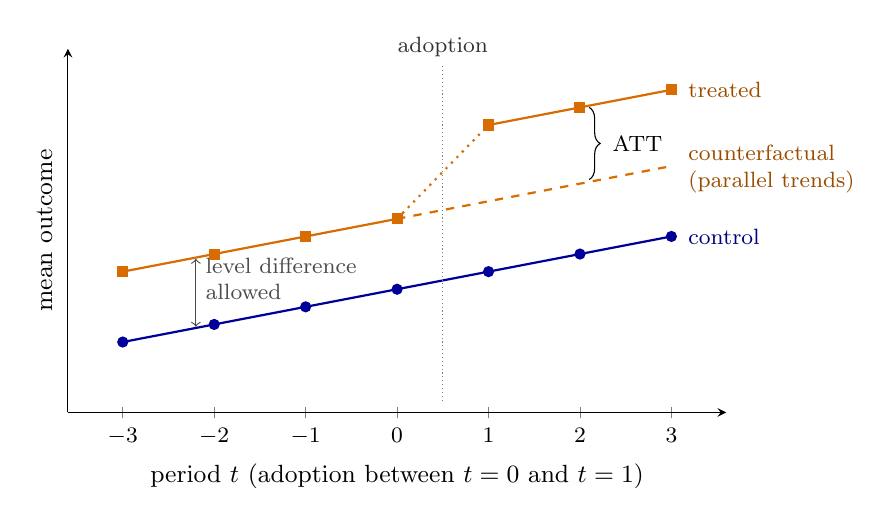
\begin{tikzpicture}
\begin{axis}[
  width=0.82\textwidth, height=6.2cm,
  xmin=-3.6, xmax=3.6, ymin=0, ymax=6.2,
  axis lines=left, xtick={-3,-2,-1,0,1,2,3}, ytick=\empty,
  xlabel={period $t$ (adoption between $t=0$ and $t=1$)}, ylabel={mean outcome},
  xlabel style={font=\small}, ylabel style={font=\small}, tick label style={font=\footnotesize},
  clip=false]
\addplot[thick, blue!60!black, mark=*, mark size=1.6pt, domain=-3:3, samples=7] {1.2+0.3*(x+3)};
\addplot[thick, orange!85!black, mark=square*, mark size=1.6pt, domain=-3:0, samples=4] {2.4+0.3*(x+3)};
\addplot[thick, orange!85!black, mark=square*, mark size=1.6pt, domain=1:3, samples=3] {2.4+0.3*(x+3)+1.3};
\addplot[thick, orange!85!black, dotted, domain=0:1, samples=2] {2.4+0.3*(x+3)+1.3*x};
\addplot[thick, dashed, orange!85!black, domain=0:3, samples=4] {2.4+0.3*(x+3)};
\draw[gray, densely dotted] (axis cs:0.5,0.2) -- (axis cs:0.5,5.9);
\node[font=\footnotesize, gray!40!black, anchor=south] at (axis cs:0.5,5.9) {adoption};
\draw[decorate, decoration={brace, mirror, amplitude=4pt}] (axis cs:2.1,3.97) -- (axis cs:2.1,5.2)
  node[midway, right=5pt, font=\footnotesize] {$\mathrm{ATT}$};
\node[font=\footnotesize, orange!60!black, anchor=west] at (axis cs:3.08,5.5) {treated};
\node[font=\footnotesize, orange!60!black, anchor=west, align=left] at (axis cs:3.08,4.15)
  {counterfactual\\(parallel trends)};
\node[font=\footnotesize, blue!50!black, anchor=west] at (axis cs:3.08,3.0) {control};
\draw[<->, gray!60!black] (axis cs:-2.2,1.46) -- (axis cs:-2.2,2.62)
  node[midway, right, yshift=5pt, font=\footnotesize, align=left] {level difference\\allowed};
\end{axis}
\end{tikzpicture}
\caption{The difference-in-differences design. Squares are the mean outcomes of the treated group and dots those
of the control group. The dashed line is the treated group's untreated path implied by parallel trends. The vertical
distance between the observed treated path and the dashed line is the average effect on the treated. Groups may
differ in levels.}
\label{fig:A-did}
\end{figure}

\subsection{Two-way fixed effects and continuous treatment}\label{sec:A-did-twfe}

With many periods, and possibly a treatment of varying intensity, the DiD regression generalizes to the
\emph{two-way fixed-effects} (TWFE) model
\begin{equation}\label{eq:A-twfe}
y_{it}=\mu_i+\tau_t+\beta\,d_{it}+e_{it},\qquad i=1,\dots,n,\quad t=1,\dots,T,
\end{equation}
where $d_{it}$ may be binary or continuous. The unit effects $\mu_i$ absorb permanent differences across units, and
the period effects $\tau_t$ absorb shocks common to all units in a period.

Let $\tilde d_{it}$ be the residual from regressing $d_{it}$ on the unit and period dummies. By the
Frisch-Waugh-Lovell theorem (\cref{thm:A-fwl}), the OLS estimate of $\beta$ equals the slope of a regression of
$y_{it}$ on $\tilde d_{it}$:
\begin{equation}\label{eq:A-twfe-fwl}
\hat\beta=\frac{\sum_{i,t}\tilde d_{it}\,y_{it}}{\sum_{i,t}\tilde d_{it}^2}.
\end{equation}
In a balanced panel the residual has the closed form already used in \cref{sec:A-panel}. Let $\bar d_i$, $\bar d_t$ and $\bar d$ be the unit, period and
overall means of $d_{it}$. Then
\begin{equation}\label{eq:A-dtilde}
\tilde d_{it}=d_{it}-\bar d_i-\bar d_t+\bar d.
\end{equation}
To verify \eqref{eq:A-dtilde}, note two facts. The difference $d_{it}-\tilde d_{it}=\bar d_i+\bar d_t-\bar d$ is a
unit term plus a period term, so it lies in the span of the dummies. And $\tilde d_{it}$ sums to zero over $t$ for
each $i$ and over $i$ for each $t$, so it is orthogonal to every dummy. These are the two properties that define the
residual of a projection.

\casehead{Identification}
Substitute \eqref{eq:A-twfe} into \eqref{eq:A-twfe-fwl}. The fixed effects drop out because
$\sum_{i,t}\tilde d_{it}(\mu_i+\tau_t)=0$, and $\sum_{i,t}\tilde d_{it}d_{it}=\sum_{i,t}\tilde d_{it}^2$ because
$\tilde d_{it}$ is orthogonal to $d_{it}-\tilde d_{it}$. Hence
\begin{equation*}
\hat\beta=\beta+\frac{\sum_{i,t}\tilde d_{it}\,e_{it}}{\sum_{i,t}\tilde d_{it}^2}.
\end{equation*}
Let $\mathbf{d}$ collect the treatments of all units in all periods. If $\E[e_{it}\mid\mathbf{d}]=0$ for every $i$
and $t$, then $\E[\hat\beta\mid\mathbf{d}]=\beta$. This \emph{strict exogeneity} condition is the multi-period form of
parallel trends and no anticipation. It allows treatment to be correlated with $\mu_i$. It rules out treatment
that responds to past or expected future shocks to the unit's outcome.

The variation that identifies $\beta$ is the change in a unit's treatment relative to the average change across
units. The two-unit, two-period case shows this transparently. Let units $A$ and $B$ be observed in two periods, and
write $\Delta y_i=y_{i2}-y_{i1}$ and $\Delta d_i=d_{i2}-d_{i1}$. First differences remove $\mu_i$:
\begin{equation*}
\Delta y_i=(\tau_2-\tau_1)+\beta\,\Delta d_i+\Delta e_i,\qquad i\in\{A,B\}.
\end{equation*}
Two equations in two unknowns fit exactly. Subtracting the equation for $B$ from that for $A$ gives
\begin{equation}\label{eq:A-wald-did}
\hat\beta=\frac{\Delta y_A-\Delta y_B}{\Delta d_A-\Delta d_B}.
\end{equation}
The estimate is the DiD in outcomes divided by the DiD in treatment. It has the form of a Wald estimator
(\cref{sec:A-iv}), with the change in treatment playing the role of the first stage.

\casehead{Sumner's tax regression as a DiD with a continuous dose}
The cigarette regression of \citet{Sumner1981}, written as \eqref{eq:A-sumner} in \cref{sec:A-panel}, is a TWFE
regression with a continuous treatment, the specific tax $t_{sy}$ of state $s$ in year $y$. The pass-through $\rho$
equals one under competition with constant marginal cost and exceeds one under market power with constant-elasticity
demand (\cref{sec:03-passthrough-theory}). By \eqref{eq:A-wald-did}, a state that raises its tax by 10 cents more than
another state identifies $\rho$ from the difference in their price changes. Sumner states the identifying assumption
directly. The remaining price variation ``is assumed to be uncorrelated with $R_{it}$'' (p.~1015), where $R_{it}$ is his
notation for the tax. He adds that the state dummies account for any stable pattern of state tax rates, such as an
effect of the unchanging location of the tobacco industry (pp.~1015--1016).

\Cref{sec:A-panel} reports his estimates. The two-way estimate of 1.074 falls to 1.029 when the year effects are
replaced by the national price index and the state effects are dropped. Cross-state differences in tax levels and
within-state tax changes therefore carry different information. The main threats to \eqref{eq:A-sumner} are tax
increases timed with changes in local demand or cost, and cross-border purchases that make legal sales respond to the
tax gap with neighboring states. Sumner checks the second by adding a squared tax term to year-by-year regressions. It
is insignificant in most years (n.~9, p.~1017). \Cref{sec:A-sumner-se} shows that the standard error of $\hat\rho$ more
than doubles once dependence within states is allowed.

\begin{remark}[Heterogeneous pass-through]\label{rem:A-twfe-hetero}
Suppose pass-through differs across states, so that $p_{sy}=\mu_s+\tau_y+\rho_s t_{sy}+e_{sy}$ with strictly
exogenous errors. Repeating the steps above gives $\E[\hat\rho\mid\mathbf{t}]=\sum_sW_s\rho_s$ with
\begin{equation*}
W_s=\frac{\sum_y\tilde t_{sy}\,t_{sy}}{\sum_{s',y}\tilde t_{s'y}^2},\qquad \sum_sW_s=1 .
\end{equation*}
In a balanced panel $\sum_y\tilde t_{sy}=0$, so we may replace $t_{sy}$ by $t_{sy}-\bar t_s$, and
$t_{sy}-\bar t_s=\tilde t_{sy}+(\bar t_y-\bar t)$ by \eqref{eq:A-dtilde}. Therefore
\begin{equation*}
W_s=\frac{\sum_y\tilde t_{sy}^2+\sum_y\tilde t_{sy}\,(\bar t_y-\bar t)}{\sum_{s',y}\tilde t_{s'y}^2}.
\end{equation*}
The first term is the state's share of the residual tax variation. The second term sums to zero across states, but
it can be negative for a state whose tax deviations move against the national path. A weight can then be negative.
\citet{CallawayGoodmanBaconSantAnna2024} show that with a continuous dose the TWFE coefficient also mixes effects at
different dose levels. Comparing units with different doses then needs a stronger assumption than parallel trends.
\end{remark}

\subsection{Control groups in IO retrospectives}\label{sec:A-did-control}

A good control group satisfies two requirements. It is subject to the same shocks as the treated group, so that
parallel trends is plausible. And it is unaffected by the treatment, so that no interference holds. In product
markets these requirements pull in opposite directions. Products that share the demand and cost shocks of the
merging products are their close substitutes, and close substitutes respond to the merger. With Bertrand
competition prices are strategic complements, so rivals raise their prices when the merged firm raises its own.
The next proposition shows what this does to the estimate.

\begin{proposition}[Partially affected controls]\label{prop:A-did-spillover}
Let (i) and (ii) of \cref{ass:A-did} hold, and suppose that the treatment raises the mean outcome of the control
group by a fraction $\kappa$ of the effect on the treated:
\begin{equation*}
\E\big[y_{i1}-y_{i1}(0)\mid\mathit{Treat}_i=0\big]=\kappa\cdot\mathrm{ATT}.
\end{equation*}
Then $\E[\hat\beta^{\mathrm{DD}}]=(1-\kappa)\mathrm{ATT}$. If $0\le\kappa<1$, the expectation of the DiD estimate has
the sign of the ATT and is no larger in magnitude. It is then a lower bound on the size of the effect. If $\kappa=1$,
the expectation is zero. If $\kappa<0$, DiD overstates the effect.
\end{proposition}

\begin{proof}
The treated-group change is as in the proof of \cref{prop:A-did}:
$\E[\bar y_{T,1}-\bar y_{T,0}]=\mathrm{ATT}+\E_1[y_{i1}(0)-y_{i0}(0)]$. For the control group, add and subtract
$\E_0[y_{i1}(0)]$ and use (i):
\begin{align*}
\E\big[\bar y_{C,1}-\bar y_{C,0}\big]
&=\E_0\big[y_{i1}-y_{i1}(0)\big]+\E_0\big[y_{i1}(0)-y_{i0}(0)\big]\\
&=\kappa\cdot\mathrm{ATT}+\E_0\big[y_{i1}(0)-y_{i0}(0)\big].
\end{align*}
Subtract the second display from the first and use (ii) to cancel the trends. The result is
$(1-\kappa)\mathrm{ATT}$. For $0\le\kappa\le1$ the factor $1-\kappa$ lies in $[0,1]$, which gives the bound. For
$\kappa<0$ the factor exceeds one.
\end{proof}

The fraction $\kappa$ has a structural interpretation. Consider a symmetric linear Bertrand oligopoly with $N$ firms,
two of which merge, with own-price demand slope $b$ and cross-price slope $d$. \Cref{prop:11-didbias} shows that each
outsider raises its price by $\kappa=\frac{2d}{2b-(N-3)d}$ times the insiders' increase. With three firms $\kappa$ equals the diversion ratio between the merging products. The bias is
therefore largest when the merging products are close substitutes, which is when the merger matters most. A
negative $\kappa$ arises for quantities. If the merged firm raises its prices, rivals gain sales, and a DiD in
quantities with rivals as controls overstates the merging firms' loss.

The opposite choice, a distant control, has the opposite problem. Store brands (private labels) use the same
inputs as branded products, and if they are supplied elastically their prices track costs while the merger leaves
them alone, so $\kappa\approx0$. But they may face different demand shocks. A rise in income can raise the demand for
branded goods relative to store brands. Then (ii) fails and the private-label estimate is biased in an unknown
direction. Reporting both control groups shows how much the conclusion depends on this trade-off. We now look at
five designs from the book. \Cref{tab:A-did-apps} summarizes them, with Sumner's design for comparison.

\casehead{Ashenfelter and Hosken (2010): two control groups}
\citet{AshenfelterHosken2010} study five consumer-product mergers that looked problematic from the public record
(\cref{sec:11-ah}).\footnote{We use the NBER working-paper version, \citet{AshenfelterHosken2008}, for page and table
numbers.} For each merging product and its control group they estimate, in logs,
\begin{equation}\label{eq:A-ah}
p_{ijt}=\alpha_{ij}+\sum_{m=1}^{11}\delta_m M_{ijt}+\beta_1\,\mathit{Post}_{ijt}
+\beta_2\,\mathit{Post}_{ijt}\times\mathit{MergingParty}_i+e_{ijt},
\end{equation}
for product $i$ in city $j$ and month $t$ (their eq.~1, p.~24). Here $\alpha_{ij}$ is a product-city fixed effect and
$M_{ijt}$ are calendar-month indicators for seasonality. The coefficient $\beta_2$ is the DiD estimate of the
proportional price change. The preferred control group is the private-label products closest to the merging brands.
The alternative is branded close substitutes, which the authors expect to understate the effect for the reason in
\cref{prop:A-did-spillover} and treat mainly as a specification check (pp.~23--24). The preferred window has equal
spans of data before and after the merger and drops the three months on each side of consummation (p.~22). Dropping
those months avoids having to date the start of joint pricing. The symmetric window guards against transitory
selection, a point first made by \citet{HeckmanRobb1985} and used by \citet{AshenfelterCard1985}
(\cref{prop:11-window}).

The aggregate effects in their Table~13 show that the control group matters (\cref{tab:11-ah}). With private-label
controls, Pennzoil and Quaker State raised prices by 0.052 log points (s.e.\ 0.013), against 0.014 (0.011) with
branded controls. For Procter and Gamble and Tambrands the figures are 0.070 (0.008) and 0.023 (0.007). Both
patterns fit \cref{prop:A-did-spillover} with $\kappa$ between zero and one. For General Mills and the Chex brands
the order reverses, 0.032 (0.005) against 0.057 (0.005). If private-label prices were unaffected and followed
parallel trends, \cref{prop:A-did-spillover} would make the branded estimate the smaller one. The reversal therefore
means that at least one control group violates the assumptions, through different trends or through store-brand
prices that responded to the merger.

\casehead{Ashenfelter, Hosken and Weinberg (2013): composition and product turnover}
\citet{AshenfelterHoskenWeinberg2013} study the 2006 Whirlpool-Maytag merger in major appliances
(\cref{sec:11-maytag}).\footnote{We use the NBER working-paper version, \citet{AshenfelterHoskenWeinberg2011}, for page
numbers.} The treated categories are dishwashers, refrigerators, clothes washers and clothes dryers. The comparison
categories are cooktops, freezers, ovens and ranges, restricted to brands not made by either party, where the merger
changed concentration little (p.~10). Their eq.~(4) (p.~12) is
\begin{equation}\label{eq:A-ahw4}
\begin{split}
\ln p_{it}={}&\beta_1\,\mathit{Maytag}_i\times\mathit{Post}_t+\beta_2\,\mathit{Whirlpool}_i\times\mathit{Post}_t\\
&+\sum_k\gamma^T_k\mathit{Age}^T_{ikt}+\sum_k\gamma^C_k\mathit{Age}^C_{ikt}+\sum_l\lambda_l\,\mathit{Month}_{lt}+\alpha_i+e_{it},
\end{split}
\end{equation}
where $i$ is a stock-keeping unit (SKU), a narrowly defined model, and $\alpha_i$ an SKU fixed effect. The age
indicators are separate for treatment and comparison categories, because appliance prices fall with a model's age at
category-specific rates. The month effects absorb common shocks.

Product turnover creates a composition problem with a sharp econometric form. For an SKU introduced after the merger,
$\mathit{Post}_t=1$ in every month it is observed. Its interaction $\mathit{Maytag}_i\times\mathit{Post}_t$ then
equals the constant $\mathit{Maytag}_i$ and is absorbed by $\alpha_i$. With SKU effects, the merger effect is
identified only from SKUs sold both before and after the merger (p.~13). Since most models live about a year, this
discards the products introduced after the merger, whose prices the merged firm chose. The authors' eq.~(5) replaces
$\alpha_i$ by observed characteristics and brand dummies, so new SKUs contribute. On SKUs introduced within a year of
the merger, eqs.~(4) and~(5) give nearly identical effects (pp.~14--15). The authors read this agreement as evidence
that unobserved SKU quality is not correlated with the post-merger indicators, given the characteristics. The preferred results
show price increases for new products in two categories. New Whirlpool dryers rose by 13 to 17 percent, depending on
the comparison category, and new Maytag dishwashers by 5 to 7 percent (p.~16). Standard errors are clustered by SKU
(p.~14).

\casehead{Bj\"ornerstedt and Verboven (2016): merging firms against rivals}
\citet{BjornerstedtVerboven2016} evaluate the acquisition of AstraZeneca Tika (AZT) by GlaxoSmithKline (GSK) in the
Swedish market for painkillers (\cref{sec:11-bv}).\footnote{Only pp.~134, 137 and 147 of the published article were
available to us. References marked WP are to the January 2013 working paper, \citet{BjornerstedtVerboven2013}. Its
printed page numbers equal its PDF page numbers minus one.} The two firms were the only sellers of paracetamol, and
the Swedish Competition Authority cleared the merger on April 3, 2009 (WP pp.~4 and~6). Their retrospective
regression, in the spirit of \eqref{eq:A-ah}, is
\begin{equation*}
\ln p_{gt}=\alpha_g+\beta_g\,\mathit{PostMerger}_t+e_{gt},
\end{equation*}
where $p_{gt}$ is the average price of product group $g$ in month $t$ (eq.~1, p.~134, and WP eq.~18). Each group
has its own post-merger change. \citet{AshenfelterHosken2010} instead give all control products a common change
(WP p.~27, n.~16). The difference between the merging group's $\beta_g$ and a rival group's $\beta_g$ is a DiD
estimate. The authors note that the merger may also raise rival prices, and the difference is then a lower bound for
the merger effect (p.~134). This is the case $0<\kappa<1$ of \cref{prop:A-did-spillover}.

The two versions of the paper use different windows. The published article defines groups by substance and by
substance and firm. It compares one year before with one year after the merger, ``to exclude possible changes after
the deregulation'' of the Swedish pharmacy monopoly (p.~134). The working paper compares April 2007 to April 2009
with May 2009 to May 2011, and reports groups by substance and by firm (WP pp.~27--28). In that longer window the
paracetamol price drifts down near the end, ``perhaps associated with new entry threats following the deregulation''
(WP p.~27). The one-year window of the published article leaves out these months.

The regression table of the published article (its Table~4, one-year window) was not available to us. We therefore
report WP Table~7, which uses the two-year window and robust standard errors. The published estimates may differ. In
log points, the post-merger change is 0.351 (0.007) for paracetamol, 0.001 (0.005) for ibuprofen and 0.100 (0.004)
for acetylsalicylic acid (ASA, sold as aspirin). The merging firms moved together, with 0.356 (0.006) for AZT and
0.379 (0.009) for GSK. With ibuprofen as the control group, the DiD estimate is 0.350 log points, or 42 percent.
With ASA as the control, it is 0.251, or 29 percent (WP p.~29). Pooling the two rival substances into one control
gives 0.30, or 35 percent (WP p.~29, n.~17). The abstract of the working paper reports these figures as an increase of 42
percent in absolute terms and 35 percent relative to rivals. The ASA increase fits $\kappa>0$, which makes the
ASA-based estimate the smaller one. The authors offer a second reason, a mandated cut in ASA package sizes (WP
p.~29). That reason is a failure of parallel trends instead. Both reasons lower the ASA-based estimate, and the
design cannot separate them.

\casehead{Dafny (2009): rival exposure, an instrument and placebo periods}
\citet{Dafny2009} measures the effect of hospital mergers on the prices of rival hospitals (\cref{sec:11-dafny}).
\Cref{sec:A-ivmodel} sets out her design. Read as a panel design, it is a first-differenced TWFE model with a
continuous treatment. The unit is a hospital that did not merge, and the outcome is the long difference in log price
from 1988 to 1997. The treatment is the number of rival mergers between 1989 and 1996, as in \eqref{eq:A-dafny-iv}.
Strict exogeneity fails here. Hospitals with merging rivals had slower price growth before the merger wave
(\cref{sec:A-potential}), so mergers happened in markets on different paths. The co-location instrument restores
identification, and \cref{tab:A-dafny} reports the first stage, the reduced form and the IV and OLS estimates.

The design borrows the event-study logic of \cref{sec:A-did-es} through placebo periods. If co-location affected
price growth through channels other than mergers, it would also predict growth before and after the merger wave.
The reduced-form coefficient is $-0.016$ (0.010) for 1985--1988 and $-0.008$ (0.013) for 1997--2000 (panel B of
\cref{tab:A-dafny}). These are tests of the exclusion restriction in the spirit of pre-trend tests.

\casehead{Whinston and Collins (1992): two cohorts as each other's controls}
\citet{WhinstonCollins1992} study incumbent responses to entry by People Express on routes out of Newark
(\cref{sec:09-wc-did}). Markets entered in 1984 and markets entered in 1985 are observed in the first quarters of
1984, 1985 and 1986. Let $D_{my}=1$ if market $m$ has been entered by year $y$, and consider
\begin{equation*}
\ln P_{my}=\mu_m+\nu_y+\beta\,D_{my}+e_{my}.
\end{equation*}
For the 1984 cohort $D$ is $(0,1,1)$ across the three years, and for the 1985 cohort it is $(0,0,1)$. In 1984--1985
the 1985 cohort, not yet entered, is the control for the 1984 cohort. In 1985--1986 the 1984 cohort, already entered,
is the control for the 1985 cohort. The incumbents' mean price fell 33 percent (s.d.\ 26) in the 1984 cohort and rose
2 percent (24) in the 1985 cohort during 1984--1985, with a two-sample $t$ statistic of 2.5. In 1985--1986 the
changes were 0 percent (15) and $-35$ percent (21), with $t=3.5$ (Table~3, p.~459). The second comparison uses an
already treated group as control. It is valid only if the 1984 cohort's effect stayed constant in its second year.
The flat 1984 cohort change in 1985--1986 supports that assumption. \Cref{sec:A-did-staggered} shows why this
condition matters in staggered designs. The authors also caution that demand or cost conditions may have changed in
the entered markets, and could even have caused entry (pp.~458--459).

\begin{remark}[DiD inside a structural model]\label{rem:A-did-structural}
\citet[pp.~1779--1780]{MillerWeinberg2017} estimate a supply model for beer that allows a departure from Nash-Bertrand
after the merger. ABI and MillerCoors may then partly or fully internalize the effect of their prices on each other's
profits. The instrument that identifies the departure is an indicator for ABI and MillerCoors products after the
merger. A separate post-merger cost shifter for MillerCoors isolates the comparison between ABI and the imported brands of Modelo and Heineken.
Identification therefore rests on a DiD comparison of implied marginal costs, which \cref{prop:11-mc-did} makes
exact. Parallel trends is then an assumption about the unobserved costs of ABI and of the imported brands.
\end{remark}

\begin{table}[htbp]
\centering
\caption{Difference-in-differences designs in the book}
\label{tab:A-did-apps}
\footnotesize
\begin{tabularx}{\textwidth}{@{}>{\raggedright\arraybackslash}p{2.05cm}>{\raggedright\arraybackslash}X>{\raggedright\arraybackslash}X>{\raggedright\arraybackslash}p{2.2cm}>{\raggedright\arraybackslash}p{1.9cm}>{\raggedright\arraybackslash}X@{}}
\toprule
Study & Treatment & Control & Window & Inference & Main threat\\
\midrule
\citet{Sumner1981} & state-year cigarette tax (continuous) & tax changes in other states, via state and year effects & annual, 1954--1978 & conventional, and random effects & taxes timed with local shocks, cross-border sales\\
\addlinespace
\citet{AshenfelterHosken2010} & five consumer-product mergers & private labels (preferred) or branded substitutes & symmetric, 3 months dropped on each side & clustered by month & rival responses, store-brand demand shocks\\
\addlinespace
\citet{AshenfelterHoskenWeinberg2013} & Whirlpool-Maytag, four appliance categories & cooktops, freezers, ovens, ranges of other brands & SKUs in their first year, monthly & clustered by SKU & product turnover and composition\\
\addlinespace
\citet{BjornerstedtVerboven2016} & paracetamol merger, Sweden, 2009 & ibuprofen and ASA groups & one year before and after (published), two years (WP) & robust s.e.\ (WP Table~7) & rival responses, ASA package sizes, deregulation\\
\addlinespace
\citet{Dafny2009} & number of rival hospital mergers, 1989--1996 & hospitals with fewer rival mergers, with a co-location instrument & long difference 1988--1997, placebos 1985--1988 and 1997--2000 & IV, Hausman test & co-location related to price growth\\
\addlinespace
\citet{WhinstonCollins1992} & People Express entry, Newark markets & markets entered in the other year & first quarters 1984, 1985, 1986 & two-sample $t$, 13 d.f. & entry timed with market shocks, changing effects\\
\bottomrule
\end{tabularx}

\smallskip
\parbox{\textwidth}{\footnotesize Notes: Entries are taken from the papers' text and tables, cited in the main
text. ASA is acetylsalicylic acid. For Bj\"ornerstedt and Verboven, the one-year window is that of the published
article (p.~134). The two-year window and the inference come from the January 2013 working paper (WP).}
\end{table}

\casehead{Which mergers are studied}
A retrospective estimates the effect of one merger. Conclusions about mergers in general also depend on which
mergers are studied, and \citet[pp.~255--256]{AskerNocke2021} list three filters. The studied mergers were
consummated, so an antitrust authority had usually cleared them, and blocked or deterred mergers are missing. They
come from industries with good data, mostly consumer-facing ones, and few concern intermediate goods. They also tend
to be large or to illustrate a phenomenon of interest. In potential-outcomes terms, an average over studied mergers is
an ATT for a selected population. It need not equal the effect of a merger that the authority would have blocked.
Their survey of retrospectives published from 2000 to 2020 finds a wide range of price effects. Some prices rose
sharply, some did not move and some fell (pp.~256--257).

\subsection{Inference}\label{sec:A-did-inference}

DiD data are panels, and panel errors are dependent. Outcomes of a unit are correlated over time, and outcomes of
units in the same period share common shocks. Which dependence matters depends on the regressors in the model. We
treat serial correlation first.

\begin{proposition}[DiD as a comparison of unit-level changes]\label{prop:A-did-collapse}
Consider a balanced panel with $T_0$ pre-periods and $T_1$ post-periods, a common adoption date, $n_1$ treated and
$n_0$ control units. Let $\Delta_i=\bar y_{i,\mathrm{post}}-\bar y_{i,\mathrm{pre}}$ be unit $i$'s change in mean
outcome. The TWFE estimate of $\beta$ in \eqref{eq:A-twfe} with $d_{it}=\mathit{Treat}_i\mathit{Post}_t$ equals
\begin{equation*}
\hat\beta=\bar\Delta_1-\bar\Delta_0,
\end{equation*}
the difference between the mean changes of treated and control units. If units are independent, then
$\Var(\hat\beta\mid\mathit{Treat})=\frac{\sigma_{\Delta,1}^2}{n_1}+\frac{\sigma_{\Delta,0}^2}{n_0}$, with
$\sigma_{\Delta,g}^2$ the variance of $\Delta_i$ in group $g$, whatever the serial correlation within units.
\end{proposition}

\begin{proof}
Let $p=\frac{n_1}{n}$ and $q=\frac{T_1}{T}$. With a common adoption date, $\bar d_i=q\,\mathit{Treat}_i$,
$\bar d_t=p\,\mathit{Post}_t$ and $\bar d=pq$. By \eqref{eq:A-dtilde},
\begin{equation*}
\tilde d_{it}=\mathit{Treat}_i\mathit{Post}_t-q\,\mathit{Treat}_i-p\,\mathit{Post}_t+pq=(\mathit{Treat}_i-p)(\mathit{Post}_t-q).
\end{equation*}
The denominator of \eqref{eq:A-twfe-fwl} is $\sum_i(\mathit{Treat}_i-p)^2\sum_t(\mathit{Post}_t-q)^2=np(1-p)\cdot Tq(1-q)$.
For the numerator, first sum over periods:
\begin{equation*}
\sum_t(\mathit{Post}_t-q)\,y_{it}=T_1(1-q)\,\bar y_{i,\mathrm{post}}-T_0\,q\,\bar y_{i,\mathrm{pre}}=Tq(1-q)\,\Delta_i,
\end{equation*}
using $T_1=qT$ and $T_0=(1-q)T$. Then sum over units:
$\sum_i(\mathit{Treat}_i-p)\Delta_i=np\bar\Delta_1-p(np\bar\Delta_1+n(1-p)\bar\Delta_0)=np(1-p)(\bar\Delta_1-\bar\Delta_0)$.
Dividing gives $\hat\beta=\bar\Delta_1-\bar\Delta_0$. The variance follows because the $\Delta_i$ are independent
across units.
\end{proof}

The proposition gives the right standard error in two equivalent ways. We may collapse the data to one change per
unit and compare means, or cluster the TWFE regression by unit (\cref{sec:A-cluster}). Conventional OLS standard errors
treat the $nT$ errors as independent, and they are too small when errors are positively autocorrelated. Suppose the
errors of each unit follow a stationary AR(1) process with coefficient $r$ and variance $\sigma^2$. The variance of a
mean of $m$ consecutive errors is
\begin{equation*}
\Var\Big(\frac{1}{m}\sum_{t=1}^{m}e_{it}\Big)=\frac{\sigma^2}{m^2}\Big[m+2\sum_{h=1}^{m-1}(m-h)\,r^h\Big]
\approx\frac{\sigma^2}{m}\cdot\frac{1+r}{1-r}
\end{equation*}
for large $m$, since $\sum_{h=-\infty}^{\infty}r^{|h|}=\frac{1+r}{1-r}$. The covariance between the pre-period and
post-period means is of order $\frac{1}{m^2}$ and becomes negligible. The independence formula therefore understates
the variance of $\Delta_i$ by a factor of about $\frac{1+r}{1-r}$, which is 9 when $r=0.8$. The standard error is
then too small by a factor of 3. This is the mechanism behind the placebo evidence of
\citet{BertrandDufloMullainathan2004} discussed in \cref{sec:A-cluster}. Clustering by state or collapsing to pre and
post means fixes the problem when there are many states.

\casehead{Few treated units}
Cluster-robust inference relies on many clusters, and in particular on many treated clusters. Retrospectives often
have one merger, or a handful of treated markets. \citet{ConleyTaber2011} use the control units' residuals to
estimate the distribution of the treated units' errors, which gives valid inference with few treated groups and
many controls. A related approach is \emph{randomization inference}. We reassign the treatment to each control unit
in turn, or to each possible set of units. For each placebo assignment $g$ we recompute the estimate $\hat\beta_g$.
The $p$-value is
\begin{equation*}
\hat p=\frac{1}{|\mathcal{G}|}\sum_{g\in\mathcal{G}}\indic\big\{|\hat\beta_g|\ge|\hat\beta|\big\},
\end{equation*}
where $\mathcal{G}$ is the set of assignments, including the actual one. The test is exact under the null of no
effect for any unit when treatment was assigned at random among the units, and approximate otherwise. The wild
cluster bootstrap of \cref{rem:A-wild-cluster} is a further option, with the caveats noted there for few treated clusters.

\casehead{Common shocks and the choice of cluster}
In \eqref{eq:A-ah} the regressor $\mathit{Post}_{ijt}$ takes the same value for all products and cities in a month,
and the model has no month effects beyond calendar-month seasonality. Common monthly shocks then make the errors of a
month correlated. As a result, the conventional variance understates the variance of $\hat\beta_1$ and $\hat\beta_2$
by the Moulton factor \citep{Moulton1987,Moulton1990} of \cref{prop:A-moulton} and \cref{lem:11-moulton}. Ashenfelter and Hosken therefore cluster on the time
period, ``because we are observing the prices of the same products in many different markets in each time period''
(\citealp[p.~25]{AshenfelterHosken2008}). The number of clusters is then the number of months in the window, so it is
modest. Equation \eqref{eq:A-ahw4} instead includes a full set of month effects, which absorb common monthly shocks.
The remaining dependence is within an SKU over time, and Ashenfelter, Hosken and Weinberg cluster by SKU. When both
forms of dependence matter, two-way clustering is available (\cref{sec:A-cluster}). Whinston and Collins compare cohort
means of market-level changes with a two-sample $t$ test with 13 degrees of freedom. That test treats markets as
independent and is exact under normality with equal variances.

\subsection{Event-study specifications}\label{sec:A-did-es}

A single DiD coefficient averages the effect over all post-treatment periods. An \emph{event study} estimates the
path of the effect by relative time. Let $E_i$ be the period in which unit $i$ adopts the treatment, with
$E_i=\infty$ for units never treated, and let $k=t-E_i$ be relative time. The canonical specification is
\begin{equation}\label{eq:A-es}
y_{it}=\mu_i+\tau_t+\sum_{k\ne-1}\phi_k\,\indic\{t-E_i=k\}+e_{it}.
\end{equation}
The coefficients $\phi_k$ for $k\ge0$ (the \emph{lags}) trace the effect $k$ periods after adoption. The coefficients
for $k\le-2$ (the \emph{leads}) measure differences before adoption, relative to the omitted period $k=-1$. Suppose
parallel trends and no anticipation hold, effects are the same for all adoption cohorts, and every relative period
has its own dummy. Suppose also that the sample contains never-treated units, or that a second lead is omitted
(\cref{prop:A-es-collinear}). Then $\phi_k=0$ for $k<0$, and $\phi_k$ equals the average effect at relative time $k$ for
$k\ge0$. \Cref{sec:A-did-staggered} shows what
goes wrong when effects differ across cohorts.

The choice of omitted period changes the meaning of every coefficient. With $k=-1$ omitted, $\phi_k$ is measured
relative to the last pre-treatment period. The patent event study in \cref{sec:05-dgg} omits the grant period $k=0$
instead (\cref{eq:05-dgg}). Its post-grant coefficients are then changes relative to the grant period, net of any
effect that occurred within it.

\begin{proposition}[Collinearity without never-treated units]\label{prop:A-es-collinear}
Suppose every unit is treated at some finite date and \eqref{eq:A-es} includes a dummy for every relative period
observed in the data. Then the unit effects, the period effects and the relative-time dummies are linearly dependent
even after one relative period is omitted, and $\phi$ is not identified without a second normalization.
\end{proposition}

\begin{proof}
For every observation exactly one relative-time dummy equals one, so
\begin{equation*}
\sum_{k}(k+1)\,\indic\{t-E_i=k\}=t-E_i+1 .
\end{equation*}
The term with $k=-1$ has coefficient zero, so the left side involves only included dummies. The right side is a
period term ($t$) plus a unit term ($1-E_i$), which lies in the span of the period and unit dummies. A nontrivial
linear combination of the regressors is therefore zero, and the regressor matrix does not have full column rank.
\end{proof}

The proposition shows that a linear trend in relative time cannot be told apart from a linear trend in calendar time
and a cohort effect. Researchers resolve it by omitting a second lead, usually the earliest, or by including
never-treated units. For a never-treated unit all dummies are zero while $t-E_i$ is undefined, so the identity
fails and the collinearity disappears.

\casehead{Binning}
Relative periods far from adoption are observed only for a few cohorts. Many studies therefore \emph{bin} the end
points: one dummy collects all $k\le\underline k$ and another all $k\ge\bar k$, as in the patent event study of
\cref{sec:05-dgg}. Binning assumes that the effect is constant within each bin. If effects keep growing beyond
$\bar k$, the misspecification contaminates the other coefficients, including the leads. \Cref{fig:A-staggered}
shows the result in a simulated panel.

\casehead{Leads as tests of parallel trends}
Estimated leads near zero are evidence for parallel trends and no anticipation. A joint Wald test of $\phi_k=0$ for
all leads is a formal version (\cref{sec:A-wald}). Two cautions apply. Pre-trend tests often have low power against
violations large enough to matter for the lags. And reporting the event study only when the test passes distorts the
distribution of the reported estimates, sometimes making the bias worse \citep{Roth2022}. \citet{RambachanRoth2023}
replace the exact assumption with bounds on post-treatment violations of parallel trends. One version, the
\emph{relative magnitudes} restriction, assumes that the change in the violation between consecutive post-periods is
at most $\bar M$ times the largest such change in the pre-period. The identified set for the effect then widens with
$\bar M$, and we can report the largest $\bar M$ at which the conclusion survives.

The placebo regressions of \citet{Dafny2009} are leads in long-difference form. The checks in
\citet{WhinstonCollins1992} play the same role. The 1985 cohort's price rose 2 percent in the year before its entry,
which supports parallel trends. The 1984 cohort's price was flat in the year after its entry, which supports a
constant effect.

\subsection{Staggered adoption with heterogeneous effects}\label{sec:A-did-staggered}

In many applications units adopt at different dates. Patents are granted molecule by molecule, mergers close at
different dates, and states change taxes in different years. This \emph{staggered adoption} design seems a natural
case for the TWFE regression \eqref{eq:A-twfe} with $d_{it}=\indic\{t\ge E_i\}$. The TWFE coefficient can badly
misrepresent the average effect when effects vary over time or across cohorts. A literature that began with
\citet{GoodmanBacon2021} and \citet{deChaisemartinDHaultfoeuille2020} shows this. \citet{RothEtAl2023} survey the
literature.

Let $e$ index adoption cohorts and define the \emph{cohort-time average effect}
\begin{equation*}
\mathrm{ATT}_e(k)=\E\big[y_{it}(1)-y_{it}(0)\mid E_i=e,\ t-E_i=k\big],\qquad k\ge0 .
\end{equation*}
We maintain parallel trends for all cohorts, including the never-treated, in all periods, and no anticipation:
$y_{it}=y_{it}(0)$ for $t<E_i$. Equivalently, untreated outcomes follow \eqref{eq:A-did-fe-model} with strictly
exogenous errors.

\begin{proposition}[TWFE as a weighted average of cell effects]\label{prop:A-twfe-weights}
Let $y_{it}=y_{it}(0)+d_{it}\Delta_{it}$, where $\Delta_{it}=y_{it}(1)-y_{it}(0)$ and untreated outcomes satisfy
\eqref{eq:A-did-fe-model} with $\E[\varepsilon_{it}\mid\mathbf{d},\Delta]=0$. Then
\begin{equation*}
\E\big[\hat\beta\mid\mathbf{d},\Delta\big]=\sum_{(i,t):\,d_{it}=1}w_{it}\,\Delta_{it},\qquad
w_{it}=\frac{\tilde d_{it}}{\sum_{(j,s):\,d_{js}=1}\tilde d_{js}},\qquad \sum_{(i,t):\,d_{it}=1}w_{it}=1 .
\end{equation*}
In a balanced panel the weight of a treated cell is proportional to $1-\bar d_i-\bar d_t+\bar d$, which is negative
when $\bar d_i+\bar d_t>1+\bar d$.
\end{proposition}

\begin{proof}
Substitute the outcome into \eqref{eq:A-twfe-fwl}. The terms $\mu_i+\tau_t$ drop out because $\tilde d_{it}$ is
orthogonal to the unit and period dummies. The error term has conditional mean zero. What remains is
\begin{equation*}
\E\big[\hat\beta\mid\mathbf{d},\Delta\big]=\frac{\sum_{i,t}\tilde d_{it}\,d_{it}\,\Delta_{it}}{\sum_{i,t}\tilde d_{it}^2}.
\end{equation*}
As shown in \cref{sec:A-did-twfe}, $\sum_{i,t}\tilde d_{it}^2=\sum_{i,t}\tilde d_{it}d_{it}=\sum_{d_{it}=1}\tilde d_{it}$.
This gives the weights and shows that they sum to one. The balanced-panel expression follows from
\eqref{eq:A-dtilde} with $d_{it}=1$.
\end{proof}

The weights are negative for treated cells of units that are treated for many periods ($\bar d_i$ large) in periods
when most units are treated ($\bar d_t$ large). These are early adopters late in the sample. A negative weight means
that a larger effect in such a cell lowers the TWFE coefficient. The next result shows where the negative weights
come from, in the smallest staggered design.

\begin{proposition}[Three groups and three periods]\label{prop:A-bacon3}
Let periods be $t=1,2,3$. An early group $E$ adopts in period 2, a late group $L$ adopts in period 3, and a group
$U$ is never treated, with population shares $\omega_E$, $\omega_L$ and $\omega_U$. Let
$S=\omega_E\omega_L+\omega_E\omega_U+\omega_L\omega_U$. Define four two-by-two DiD estimators from the group-period
means $\bar y_{gt}$:
\begin{align*}
\hat\beta_{EU}&=\Big(\frac{\bar y_{E2}+\bar y_{E3}}{2}-\bar y_{E1}\Big)-\Big(\frac{\bar y_{U2}+\bar y_{U3}}{2}-\bar y_{U1}\Big),\\
\hat\beta_{LU}&=\Big(\bar y_{L3}-\frac{\bar y_{L1}+\bar y_{L2}}{2}\Big)-\Big(\bar y_{U3}-\frac{\bar y_{U1}+\bar y_{U2}}{2}\Big),\\
\hat\beta^{E}_{EL}&=\big(\bar y_{E2}-\bar y_{E1}\big)-\big(\bar y_{L2}-\bar y_{L1}\big),\\
\hat\beta^{L}_{EL}&=\big(\bar y_{L3}-\bar y_{L2}\big)-\big(\bar y_{E3}-\bar y_{E2}\big).
\end{align*}
The first two compare each adopting group with the never-treated group. The third compares the early group with the
late group before the late group adopts. The fourth compares the late group with the early group after the early
group has adopted. Then the TWFE estimate is
\begin{equation*}
\hat\beta=\frac{\omega_E\omega_U}{S}\,\hat\beta_{EU}+\frac{\omega_L\omega_U}{S}\,\hat\beta_{LU}
+\frac{\omega_E\omega_L}{2S}\,\hat\beta^{E}_{EL}+\frac{\omega_E\omega_L}{2S}\,\hat\beta^{L}_{EL},
\end{equation*}
and the four weights sum to one.
\end{proposition}

\begin{proof}
Normalize $\omega_E+\omega_L+\omega_U=1$. Because treatment varies only by group and period, \eqref{eq:A-twfe-fwl}
can be computed from group-period means: $\hat\beta=\frac{\sum_{g,t}\omega_g\tilde d_{gt}\bar y_{gt}}{\sum_{g,t}\omega_g\tilde d_{gt}^2}$,
with $\tilde d_{gt}=d_{gt}-\bar d_g-\bar d_t+\bar d$. We prove the identity in three steps.

\emph{Step 1: both sides ignore additive effects.} Adding $a_g+b_t$ to every $\bar y_{gt}$ leaves $\hat\beta$
unchanged, because $\tilde d_{gt}$ is orthogonal to group and period terms. It leaves each two-by-two estimator
unchanged, because each is a difference of changes over the same periods.

\emph{Step 2: a basis.} Any array of cell means can be written as
$\bar y_{gt}=(\bar y_{g1}+\bar y_{Ut}-\bar y_{U1})+r_{gt}$, where $r_{gt}=\bar y_{gt}-\bar y_{g1}-\bar y_{Ut}+\bar y_{U1}$.
The first part is additive, and $r_{gt}=0$ in row $U$ and in column $t=1$. So $r$ is a combination of the four
indicator arrays of the cells $(E,2)$, $(E,3)$, $(L,2)$ and $(L,3)$. By Step 1 and linearity, it suffices to check
the identity for these four indicator arrays. If $\omega_U=0$, the cells of row $U$ enter neither side, and we may
give them any values.

\emph{Step 3: the four checks.} The group means of treatment are $\bar d_E=\frac{2}{3}$, $\bar d_L=\frac{1}{3}$ and
$\bar d_U=0$. The period means are $\bar d_1=0$, $\bar d_2=\omega_E$ and $\bar d_3=\omega_E+\omega_L$, and
$\bar d=\frac{2\omega_E+\omega_L}{3}$. Hence
\begin{align*}
\tilde d_{E2}&=\frac{1-\omega_E+\omega_L}{3}, & \tilde d_{E3}&=\frac{1-\omega_E-2\omega_L}{3},\\
\tilde d_{L2}&=\frac{-1-\omega_E+\omega_L}{3}, & \tilde d_{L3}&=\frac{2-\omega_E-2\omega_L}{3}.
\end{align*}
The denominator equals $\sum_{g,t}\omega_g\tilde d_{gt}d_{gt}$, a sum over the treated cells:
\begin{equation*}
\omega_E\big(\tilde d_{E2}+\tilde d_{E3}\big)+\omega_L\tilde d_{L3}
=\frac{2\omega_E+2\omega_L-2\omega_E^2-2\omega_E\omega_L-2\omega_L^2}{3}=\frac{2S}{3},
\end{equation*}
where the last step uses $S=\omega_E\omega_L+(\omega_E+\omega_L)(1-\omega_E-\omega_L)$. For the indicator of
cell $(h,s)$ the left side is $\frac{\omega_h\tilde d_{hs}}{\frac{2S}{3}}$. For the indicator of $(E,2)$ the left side
is $\frac{\omega_E(1-\omega_E+\omega_L)}{2S}$. On the right side $\hat\beta_{EU}=\frac{1}{2}$,
$\hat\beta_{LU}=0$, $\hat\beta^{E}_{EL}=1$ and $\hat\beta^{L}_{EL}=1$, so the right side is
\begin{equation*}
\frac{\omega_E\omega_U}{2S}+\frac{\omega_E\omega_L}{2S}+\frac{\omega_E\omega_L}{2S}
=\frac{\omega_E(\omega_U+2\omega_L)}{2S}=\frac{\omega_E(1-\omega_E+\omega_L)}{2S}.
\end{equation*}
For $(E,3)$ the two-by-two values are $\frac{1}{2}$, $0$, $0$ and $-1$, so both sides equal
$\frac{\omega_E(\omega_U-\omega_L)}{2S}=\frac{\omega_E(1-\omega_E-2\omega_L)}{2S}$. For $(L,3)$ the values are
$0$, $1$, $0$ and $1$, so the right side is $\frac{2\omega_L\omega_U+\omega_E\omega_L}{2S}=\frac{\omega_L(2-\omega_E-2\omega_L)}{2S}$,
which equals the left side. For $(L,2)$ the values are $0$, $-\frac{1}{2}$, $-1$ and $-1$, so the right side is
$-\frac{\omega_L(\omega_U+2\omega_E)}{2S}=\frac{\omega_L(-1-\omega_E+\omega_L)}{2S}$, which again equals the left
side. Finally, the weights sum to $\frac{2\omega_E\omega_U+2\omega_L\omega_U+2\omega_E\omega_L}{2S}=1$.
\end{proof}

The proposition says that TWFE is a weighted average of all two-by-two comparisons in the data. Three of them are
clean, in the sense that the control group is untreated in both periods compared. The fourth, $\hat\beta^{L}_{EL}$,
uses the already treated early group as the control. Its expectation reveals the problem.

\begin{corollary}[Weights on the cohort effects]\label{cor:A-bacon3}
Under parallel trends and no anticipation, in the design of \cref{prop:A-bacon3},
\begin{align*}
\E\big[\hat\beta^{L}_{EL}\big]&=\mathrm{ATT}_L(0)-\big[\mathrm{ATT}_E(1)-\mathrm{ATT}_E(0)\big],\\
\E\big[\hat\beta\big]&=\frac{\omega_E(\omega_U+2\omega_L)}{2S}\,\mathrm{ATT}_E(0)
+\frac{\omega_E(\omega_U-\omega_L)}{2S}\,\mathrm{ATT}_E(1)+\frac{\omega_L(2\omega_U+\omega_E)}{2S}\,\mathrm{ATT}_L(0).
\end{align*}
With equal shares the weights are $\frac{1}{2}$, $0$ and $\frac{1}{2}$. Without a never-treated group
($\omega_U=0$) they are $1$, $-\frac{1}{2}$ and $\frac{1}{2}$.
\end{corollary}

\begin{proof}
Under the assumptions, the expected cell means are additive effects plus $\mathrm{ATT}_E(0)$ in cell $(E,2)$,
$\mathrm{ATT}_E(1)$ in cell $(E,3)$ and $\mathrm{ATT}_L(0)$ in cell $(L,3)$. The additive effects drop out of every
estimator. The expectation of $\hat\beta^{L}_{EL}$ is $\mathrm{ATT}_L(0)-0$ for the late group minus
$\mathrm{ATT}_E(1)-\mathrm{ATT}_E(0)$ for the early group. The weights on the three effects are the left sides
computed in Step~3 of the proof of \cref{prop:A-bacon3} for the three treated cells. Setting
$\omega_E=\omega_L=\omega_U=\frac{1}{3}$ gives $S=\frac{1}{3}$ and the weights $\frac{1}{2}$, $0$, $\frac{1}{2}$.
Setting $\omega_U=0$ gives $S=\omega_E\omega_L$ and the weights $1$, $-\frac{1}{2}$, $\frac{1}{2}$.
\end{proof}

The forbidden comparison subtracts the growth of the early group's effect. If effects are constant over time,
$\mathrm{ATT}_E(1)=\mathrm{ATT}_E(0)$ and every comparison is unbiased for some average effect. If effects grow, the
comparison is biased downward and can be negative even though every effect is positive. Without a never-treated group
the extreme case is stark. Let $\mathrm{ATT}_E(0)=\mathrm{ATT}_L(0)=0$ and $\mathrm{ATT}_E(1)=1$, so that the
treatment works with a one-period lag. Then $\E[\hat\beta]=-\frac{1}{2}$, although no unit is harmed. This is the
situation Whinston and Collins guard against by checking that the 1984 cohort's effect was constant.

\begin{theorem}[Goodman-Bacon decomposition]\label{thm:A-bacon}
Consider a balanced panel with periods $t=1,\dots,T$, adoption cohorts $k$ with shares $\omega_k$ that adopt at
different dates, and possibly a never-treated group $U$ with share $\omega_U$. Let $\bar d_k$ be the fraction of
periods in which cohort $k$ is treated, and $\hat V^d=\frac{1}{nT}\sum_{i,t}\tilde d_{it}^2$. Then
\begin{equation*}
\hat\beta=\sum_k s_{kU}\hat\beta_{kU}+\sum_{k}\sum_{\ell:\,\bar d_\ell<\bar d_k}\Big(s^{k}_{k\ell}\hat\beta^{k}_{k\ell}+s^{\ell}_{k\ell}\hat\beta^{\ell}_{k\ell}\Big),
\end{equation*}
where $\hat\beta_{kU}$ compares cohort $k$ with the never-treated over all periods. The estimator
$\hat\beta^{k}_{k\ell}$ compares the earlier cohort $k$ with the later cohort $\ell$ before $\ell$ adopts, and
$\hat\beta^{\ell}_{k\ell}$ compares $\ell$ with $k$ after $k$ has adopted. The weights
\begin{equation*}
s_{kU}=\frac{\omega_k\omega_U\bar d_k(1-\bar d_k)}{\hat V^d},\qquad
s^{k}_{k\ell}=\frac{\omega_k\omega_\ell(\bar d_k-\bar d_\ell)(1-\bar d_k)}{\hat V^d},\qquad
s^{\ell}_{k\ell}=\frac{\omega_k\omega_\ell\,\bar d_\ell(\bar d_k-\bar d_\ell)}{\hat V^d}
\end{equation*}
are positive and sum to one.
\end{theorem}

We state the weights of \citet{GoodmanBacon2021}, Theorem~1, after simplifying the products of group shares. In the
design of \cref{prop:A-bacon3}, $\bar d_E=\frac{2}{3}$, $\bar d_L=\frac{1}{3}$ and $\hat V^d=\frac{2S}{9}$, and the
formulas reproduce its weights. On the simulated panel below, the script also checks that the weights sum to one and
that the weighted sum of the nine two-by-two estimates equals $\hat\beta$ to six decimals. The weights grow with group size and with the variance of treatment within each
comparison. Comparisons in which treatment switches in the middle of the window receive the most weight. The
decomposition shows that the TWFE coefficient is a variance-weighted average of comparisons. Some of these use
already treated units as controls. Every weight is positive, yet the implied weights on the cohort effects can be
negative, as in \cref{cor:A-bacon3}.

\casehead{Event studies under heterogeneity}
The dynamic specification \eqref{eq:A-es} has a related problem. \citet{SunAbraham2021} show that each TWFE
coefficient $\phi_k$ equals a weighted average of cohort effects at relative time $k$ plus a weighted sum of cohort
effects at other relative times. The second set of weights sums to zero across cohorts. Contamination therefore
vanishes when effects are the same in every cohort, and it appears when they differ. Binned or omitted relative
periods with nonzero effects add more contamination. Leads can then look like pre-trends even when parallel trends
holds.

\casehead{Heterogeneity-robust estimators}
The remedy is to estimate each cohort-time effect from clean comparisons and then average with chosen weights.
\begin{itemize}
\item \citet{CallawaySantAnna2021} estimate the group-time effect of cohort $e$ in period $t\ge e$ by a two-by-two
comparison with base period $e-1$. The estimator is
\begin{equation*}
\widehat{\mathrm{ATT}}(e,t)=\big(\bar y_{e,t}-\bar y_{e,e-1}\big)-\big(\bar y_{C,t}-\bar y_{C,e-1}\big),
\end{equation*}
where $C$ is the never-treated group or the units not yet treated by period $t$. Under parallel trends and no
anticipation, the expected change of the control group equals the change cohort $e$ would have had without
treatment, so the estimator is unbiased for $\mathrm{ATT}_e(t-e)$. Event-study estimates average these effects
across cohorts at each relative time, $\hat\phi_k=\sum_e w_e(k)\widehat{\mathrm{ATT}}(e,e+k)$, with $w_e(k)$ the
cohort shares among the cohorts observed at $k$. Leads are computed the same way for $t<e$.
\item \citet{SunAbraham2021} estimate a saturated regression with a dummy for each cohort and relative period,
using never-treated or last-treated units as controls, and average the coefficients with cohort shares. In a
balanced panel without covariates and with never-treated controls, their estimates coincide with those of Callaway
and Sant'Anna. Our simulation below confirms this to machine precision.
\item \citet{BorusyakJaravelSpiess2024} propose an \emph{imputation} estimator. It estimates $\mu_i$ and $\tau_t$
from untreated observations only, imputes $\hat y_{it}(0)=\hat\mu_i+\hat\tau_t$ for treated observations, and
averages $y_{it}-\hat y_{it}(0)$ over the cells of interest. It uses all pre-treatment periods, which makes it
efficient when errors are homoskedastic and serially uncorrelated. It leans more on parallel trends in early
periods.
\item \emph{Stacked} DiD \citep{CengizEtAl2019} builds one dataset per cohort, containing the cohort and units not
treated within a window around its adoption date. It stacks the datasets and estimates an event study with
dataset-specific unit and period effects.
\end{itemize}
These estimators differ in the control group, the base period and the weights. Each removes the forbidden
comparisons.

\casehead{A simulated illustration}
\Cref{fig:A-staggered} reports a Monte Carlo experiment. A balanced panel has 400 units observed for 20 periods.
Cohorts of 100 units adopt in periods 5, 10 and 15, and 100 units are never treated. Untreated outcomes follow
\eqref{eq:A-did-fe-model}, so parallel trends and no anticipation hold exactly. The effect $k$ periods after
adoption is $\gamma_e(k+1)$, with $\gamma_e$ equal to 0.10, 0.06 and 0.03 for the three cohorts. Effects therefore
grow with time since adoption and are larger for early cohorts. The average effect over all treated unit-periods is
0.551. The static TWFE coefficient averages 0.126 across 500 replications (standard deviation 0.020), less than a
quarter of the average effect.

Panel (b) shows why. The Goodman-Bacon decomposition of the expected TWFE coefficient puts a total weight of 0.497 on
comparisons with the never-treated group, whose weighted average is 0.400. Comparisons of earlier cohorts with
not-yet-treated cohorts receive 0.211 and average 0.344. Comparisons of later cohorts with already treated ones
receive 0.292 and average $-0.501$. The three comparisons in this last group are all negative. Their controls are
early cohorts whose effects keep rising, and the rise is subtracted from the late cohorts' effects.

Panel (a) shows the event study. The TWFE specification, with binned end points beyond $\pm5$, produces leads that
rise to 0.110 at $k=-5$, a spurious pre-trend. Its lags are too low at adoption and from $k=3$ on, reaching 0.263 at
$k=5$ where the true value is 0.380. The Callaway-Sant'Anna and imputation estimators are centered on the truth, at 0.384
and 0.383 for $k=5$. Their 5th to 95th percentile ranges at $k=5$ are $[0.293, 0.478]$ and $[0.314, 0.454]$. The
imputation estimator is more precise here because the errors are independent and homoskedastic, which is the case
in which it is efficient.

\begin{figure}[htbp]
\centering
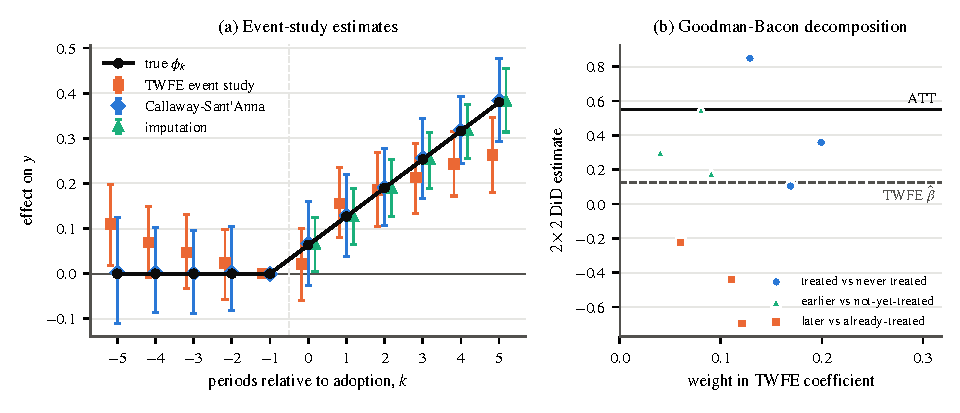
\includegraphics[width=\textwidth]{figures/appA/staggered.pdf}
\caption{Staggered adoption with effects that grow over time and differ across cohorts. (a) Mean estimates
of the event-time effects over 500 replications, with bars from the 5th to the 95th percentile. The black line is
the true effect, averaged over the cohorts observed at each relative time. The TWFE event study includes dummies
for $k=-5,\dots,5$ (omitting $k=-1$) and binned end points. (b) Goodman-Bacon decomposition of the expected
static TWFE coefficient (dashed line). Each marker is one two-by-two comparison. The solid line is the average effect
over all treated unit-periods. The design has 400 units, 20 periods, adoption in periods 5, 10 and 15 plus a never-treated
group. Numbers from \texttt{staggered\_did.py}, seed 20261022.}
\label{fig:A-staggered}
\end{figure}

The lesson for applied work is direct. When treatment timing varies and effects may change with exposure, we
should report heterogeneity-robust estimates alongside, or instead of, TWFE. The Goodman-Bacon decomposition is a
useful diagnostic, because it shows how much weight the forbidden comparisons receive. In merger retrospectives that
pool mergers closing at different dates, and in patent or entry studies with staggered timing, the issue arises
whenever the effect builds up gradually.

\subsection{Related designs}\label{sec:A-did-related}

\casehead{Synthetic control}
Many IO questions concern a single treated unit, such as the local market of one merger or one state's regulation.
With one treated unit, the choice of control group carries the whole design. The \emph{synthetic control} method
\citep{AbadieGardeazabal2003,AbadieDiamondHainmueller2010} builds the control as a weighted average of untreated
units. Let unit 1 be treated after period $T_0$ and units $2,\dots,J+1$ be potential controls. Let $X_1$ be a vector
of pre-treatment characteristics of the treated unit, including pre-period outcomes, and $X_0$ the matrix of the same
characteristics for the controls. The weights solve
\begin{equation*}
\min_{w}\ \big\|X_1-X_0w\big\|_V\quad\text{subject to}\quad w_j\ge0,\ \ \sum_{j=2}^{J+1}w_j=1,
\end{equation*}
for a positive definite weighting matrix $V$ chosen to fit pre-period outcomes. The estimated effect in period
$t>T_0$ is $y_{1t}-\sum_jw_jy_{jt}$. The constraints rule out extrapolation, because the synthetic unit lies in the
convex hull of the controls. The method is credible when the synthetic unit tracks the treated unit closely over a
long pre-period. Inference uses placebo assignments, applying the method to each control unit in turn and comparing
the treated unit's post-period gap with the placebo gaps. \citet{Abadie2021} discusses data requirements and
practice.

\casehead{Triple differences}
When the control group may face different trends, a third difference can remove them. Suppose a merger affects
product category $A$ in region 1, and region 2 and category $B$ are unaffected. The \emph{triple difference} is
\begin{equation*}
\hat\beta^{\mathrm{DDD}}=\big[\Delta\bar y_{A1}-\Delta\bar y_{A2}\big]-\big[\Delta\bar y_{B1}-\Delta\bar y_{B2}\big],
\end{equation*}
where $\Delta\bar y_{cr}$ is the change in the mean outcome of category $c$ in region $r$. The first bracket is a
regional DiD for category $A$. The second removes region-specific trends that also appear in category $B$. The
identifying assumption is that the gap between the regional trends would have been the same in both categories.
This is weaker than parallel trends for either DiD alone.

\casehead{Regression discontinuity}
When treatment is assigned by a known rule based on a running variable $z_i$, with $d_i=\indic\{z_i\ge c\}$, units
just above and just below the cutoff $c$ are comparable. If potential outcomes are continuous in $z$ at $c$, the
jump $\lim_{z\downarrow c}\E[y_i\mid z_i=z]-\lim_{z\uparrow c}\E[y_i\mid z_i=z]$ identifies the average effect at
the cutoff. Estimation uses local linear regression on each side (\cref{sec:A-loclin}). \citet{LeeLemieux2010} survey
the design. \citet{AtheyLevinSeira2011} discuss a deterministic rule for the format of timber sales, such as an open
auction whenever timber volume exceeds a threshold. Under such a rule their comparison would be identified in a
manner analogous to a regression discontinuity design (n.~13, p.~229).

\casehead{Selection on observables and matching}
A different design drops the panel. It assumes \emph{unconfoundedness}, that treatment is as good as random given
observed covariates: $(y_i(0),y_i(1))\perp d_i\mid x_i$. It also assumes \emph{overlap}, $0<\psi(x)<1$, where
$\psi(x)=\Pr(d_i=1\mid x_i=x)$ is the \emph{propensity score}. \citet{RosenbaumRubin1983} show that unconfoundedness given
$x_i$ implies unconfoundedness given $\psi(x_i)$. The proof is short. By iterated expectations,
\begin{equation*}
\Pr\big(d_i=1\mid y_i(0),y_i(1),\psi(x_i)\big)=\E\big[\Pr(d_i=1\mid y_i(0),y_i(1),x_i)\mid y_i(0),y_i(1),\psi(x_i)\big]=\psi(x_i),
\end{equation*}
because the inner probability equals $\psi(x_i)$ by unconfoundedness. Comparisons may therefore condition on the
scalar $\psi$ instead of the whole vector $x$. Estimators include regression adjustment, inverse propensity
weighting and matching. A matching estimator imputes each unit's missing potential outcome by the average outcome of
its $M$ nearest neighbors in the other treatment group. \citet{AbadieImbens2006} derive its large-sample distribution
and a consistent variance estimator. \citet{ImbensRubin2015} give a full treatment.

\citet{AtheyLevinSeira2011} use these tools to compare sealed-bid and open timber auctions held by the US Forest
Service (\cref{ch:auction-empirics}). Their sales took place between 1982 and 1990 in the Northern forests and between
1982 and 1989 in California. For an outcome $Y$ they write $Y=f(\mathit{SEALED},X,N,\epsilon)$
and target the average effect $\Delta Y=\E[f(1,X,N,\epsilon)-f(0,X,N,\epsilon)]$ (eq.~5, p.~229). The identifying
assumption is that the auction format is independent of $\epsilon$ given the covariates. It holds by design for sales
whose format was randomized, and for other sales if the format was chosen on information in their data. They
estimate a logit propensity score of the sealed-bid format on tract characteristics and drop sales with predicted
probabilities below 0.075 or above 0.925 to enforce overlap (p.~227). Their matching estimator is
\begin{equation*}
\widehat{\Delta Y}=\frac{1}{T}\sum_{t\ \text{sealed}}\big(Y_t-\hat Y_t\big)+\frac{1}{T}\sum_{t\ \text{open}}\big(\hat Y_t-Y_t\big)
\end{equation*}
(eq.~7, p.~230). Here $T$ is the number of sales, and $\hat Y_t$ is the average outcome of the $M=4$ sales of the
other format with the closest propensity scores. Standard errors follow \citet{AbadieImbens2006}. \Cref{tab:A-als}
compares the matching estimates with two regression estimates. In the Northern forests the three estimators agree
closely. Sealed bidding raises logger entry by about 10 percent and the sale price by 9 to 12 percent. In
California the price effects are small and insignificant, and the matching estimates are imprecise. Trimming for
overlap kept only a third of the California sales (p.~227). The authors also report similar estimates on the 378 Northern sales whose format
was randomized (p.~226).

\begin{table}[htbp]
\centering
\caption{Effect of sealed bidding on timber sale outcomes: regression and matching}
\label{tab:A-als}
\footnotesize
\begin{tabular}{@{}lcccc@{}}
\toprule
& \multicolumn{2}{c}{Northern forests ($N=1{,}071$)} & \multicolumn{2}{c}{California ($N=707$)}\\
\cmidrule(lr){2-3}\cmidrule(l){4-5}
Estimator & $\ln$(logger entry) & $\ln$(price) & $\ln$(logger entry) & $\ln$(price)\\
\midrule
OLS, no interactions & 0.089 & 0.094 & 0.101 & 0.027\\
 & (0.036) & (0.038) & (0.045) & (0.051)\\
OLS with sealed $\times$ covariate interactions & 0.097 & 0.099 & 0.099 & 0.026\\
 & (0.036) & (0.039) & (0.044) & (0.050)\\
Propensity-score matching, $M=4$ & 0.100 & 0.118 & 0.106 & $-0.038$\\
 & (0.048) & (0.064) & (0.062) & (0.127)\\
\bottomrule
\end{tabular}

\smallskip
\parbox{0.92\linewidth}{\footnotesize Notes: Each entry is the estimated effect of the sealed-bid format, with robust
standard errors in parentheses (Abadie-Imbens standard errors for matching). Regressions control for the Forest
Service appraisal variables, sale characteristics and year, quarter and location dummies. Samples exclude sales with
propensity scores outside $[0.075,0.925]$. Source: \citet{AtheyLevinSeira2011}, Table~III, columns 1 and 5.}
\end{table}

\section{Financial event studies}\label{sec:A-eventstudy}

A financial \emph{event study} measures the effect of a discrete piece of news on the market value of firms. The
method goes back to \citet{FamaEtAl1969}, and \citet{MacKinlay1997} surveys it. Industrial organization uses it to
learn about profits that we cannot observe directly. A merger that raises market power should raise the value of the
merging firms' rivals, and entry into a profitable market should lower the value of incumbents. This section
develops the method in general form. \Cref{sec:09-wc-method} applies it in full to the entry study of
\citet{WhinstonCollins1992}, and \cref{sec:11-retro-event} applies it to mergers.

\subsection{Premise}\label{sec:A-es-premise}

The method rests on \emph{market efficiency}. The equity value of a firm equals the expected present value of the
cash flows to its shareholders, given all public information. When news changes expected future profits, the share
price adjusts as soon as the news becomes public. The return on the announcement day, net of the return the stock
would have earned anyway, then measures the revision in the expected value of the firm to its shareholders. A study
of a few days of returns can thus reveal a change in discounted profits over many years. The price of this economy is
a set of assumptions about information, timing and the model of normal returns, which we make explicit below.

\subsection{Normal returns and abnormal returns}\label{sec:A-es-ar}

Index firms by $f$ and trading days by $\tau$, with the announcement on day $\tau=0$ of \emph{event time}. Let
$R_{f\tau}$ be the return on firm $f$'s stock, including dividends, $R^m_\tau$ the return on a market index and
$R^0_\tau$ the risk-free rate. The \emph{normal return} is the return expected without the event. Three models are
common. The \emph{constant-mean model} sets $R_{f\tau}=\mu_f+u_{f\tau}$. The \emph{market model} sets
\begin{equation}\label{eq:A-es-mm}
R_{f\tau}=a_f+b_f R^m_\tau+u_{f\tau},\qquad \E[u_{f\tau}\mid R^m]=0,\quad \Var(u_{f\tau}\mid R^m)=\sigma_f^2,
\end{equation}
with errors uncorrelated across days. The \emph{excess-return} form of the capital asset pricing model replaces
returns by returns in excess of the risk-free rate,
$R_{f\tau}-R^0_\tau=a_f+b_f(R^m_\tau-R^0_\tau)+u_{f\tau}$, as in \cref{sec:09-wc-method}. The market model removes the
part of the return due to market-wide news, which reduces the variance of the abnormal return and raises power.

The model is estimated on an \emph{estimation window} of $T_e$ trading days that ends some days before the event,
so that the event cannot affect the estimates. The \emph{event window} is $[\tau_1,\tau_2]$, which contains day
0 and has $L=\tau_2-\tau_1+1$ days. Days before the announcement allow for leakage, and days after it allow for slow
absorption. \Cref{fig:A-es-timeline} shows the layout.

\begin{figure}[htbp]
\centering
\begin{tikzpicture}[x=1cm,y=1cm]
\draw[-{Stealth[length=2.4mm]}, thick] (0,0) -- (14.2,0);
\node[font=\footnotesize, anchor=north east] at (14.2,-0.15) {event time $\tau$};
\fill[blue!18] (0.3,-0.14) rectangle (6.3,0.14);
\fill[gray!15] (6.3,-0.14) rectangle (7.9,0.14);
\fill[orange!35] (7.9,-0.14) rectangle (10.3,0.14);
\fill[gray!30] (10.3,-0.14) rectangle (13.4,0.14);
\foreach \x/\lab in {0.3/{\tau_1-g-T_e}, 6.3/{\tau_1-g-1}, 7.9/{\tau_1}, 9.1/{0}, 10.3/{\tau_2}} {
  \draw (\x,0.18) -- (\x,-0.18);
  \node[font=\footnotesize, below] at (\x,-0.2) {$\lab$};
}
\node[font=\footnotesize, anchor=north] at (9.1,-0.62) {(announcement)};
\draw[decorate, decoration={brace, amplitude=5pt}] (0.3,0.3) -- (6.3,0.3)
  node[midway, above=6pt, font=\footnotesize, align=center] {estimation window\\$T_e$ days: estimate $a_f$, $b_f$, $\sigma_f^2$};
\draw[decorate, decoration={brace, amplitude=4pt}] (6.35,0.3) -- (7.85,0.3)
  node[midway, above=5pt, font=\footnotesize] {gap, $g$ days};
\draw[decorate, decoration={brace, amplitude=5pt}] (7.9,0.3) -- (10.3,0.3)
  node[midway, above=6pt, font=\footnotesize, align=center] {event window\\$L$ days};
\draw[decorate, decoration={brace, mirror, amplitude=5pt}] (10.7,-0.85) -- (13.4,-0.85)
  node[midway, below=6pt, font=\footnotesize] {post-event window};
\end{tikzpicture}
\caption{Windows in a financial event study. The normal-return model is estimated on the estimation window, which
ends $g$ days before the event window so that the event cannot affect the estimates. Abnormal returns are computed
on the event window $[\tau_1,\tau_2]$ around the announcement on day 0. A post-event window can be used to check for
slow adjustment.}
\label{fig:A-es-timeline}
\end{figure}

\begin{definition}[Abnormal and cumulative abnormal returns]\label{def:A-es-ar}
Let $(\hat a_f,\hat b_f)$ be the OLS estimates of \eqref{eq:A-es-mm} on the estimation window. The \emph{abnormal
return} on an event-window day is the prediction error
$AR_{f\tau}=R_{f\tau}-\hat a_f-\hat b_fR^m_\tau$. The \emph{cumulative abnormal return} is
$CAR_f(\tau_1,\tau_2)=\sum_{\tau=\tau_1}^{\tau_2}AR_{f\tau}$.
\end{definition}

The variance of abnormal returns has a compact matrix form. Stack the estimation-window data as $y_e$ ($T_e\times1$)
and $X_e=[\iota,\,R^m_e]$ ($T_e\times2$), and the event-window data as $y^*$ ($L\times1$) and $X^*$ ($L\times2$). Let
$AR^*$ be the $L\times1$ vector of abnormal returns.

\begin{proposition}[Variance of abnormal returns]\label{prop:A-es-arvar}
Suppose that \eqref{eq:A-es-mm} holds on both windows under the null hypothesis of no event effect. Let the errors
be independent of the market returns and uncorrelated across days, with variance $\sigma_f^2$. Then, conditional on
the market returns,
\begin{equation*}
\E\big[AR^*\big]=0,\qquad \Var\big(AR^*\big)=\sigma_f^2\Big[I_L+X^*(X_e^\top X_e)^{-1}X^{*\top}\Big].
\end{equation*}
For a single day,
\begin{equation*}
\Var\big(AR_{f\tau}\big)=\sigma_f^2\left[1+\frac{1}{T_e}+\frac{(R^m_\tau-\hat\mu_m)^2}{\sum_{s}(R^m_s-\hat\mu_m)^2}\right],
\end{equation*}
where $\hat\mu_m$ is the mean market return over the estimation window and the sum runs over it. For the
cumulative abnormal return, $\Var(CAR_f)=\iota^\top\Var(AR^*)\,\iota$.
\end{proposition}

\begin{proof}
Write $\theta_f=(a_f,b_f)^\top$ and $\hat\theta_f=(X_e^\top X_e)^{-1}X_e^\top y_e$. Under the null,
$y^*=X^*\theta_f+u^*$, so
\begin{equation*}
AR^*=y^*-X^*\hat\theta_f=u^*-X^*(\hat\theta_f-\theta_f)=u^*-X^*(X_e^\top X_e)^{-1}X_e^\top u_e .
\end{equation*}
Both terms have mean zero. The event-window errors $u^*$ are uncorrelated with the estimation-window errors $u_e$,
so the variance is the sum of $\Var(u^*)=\sigma_f^2I_L$ and
\begin{equation*}
X^*(X_e^\top X_e)^{-1}X_e^\top\Var(u_e)X_e(X_e^\top X_e)^{-1}X^{*\top}=\sigma_f^2X^*(X_e^\top X_e)^{-1}X^{*\top}.
\end{equation*}
For a single day with regressor row $x_\tau=(1,R^m_\tau)$, write $Q=\sum_s(R^m_s-\hat\mu_m)^2$. The inverse is
\begin{equation*}
(X_e^\top X_e)^{-1}=\frac{1}{T_eQ}\begin{pmatrix}\sum_s(R^m_s)^2 & -\sum_sR^m_s\\ -\sum_sR^m_s & T_e\end{pmatrix}.
\end{equation*}
Then $x_\tau(X_e^\top X_e)^{-1}x_\tau^\top=\frac{\sum_s(R^m_s)^2-2R^m_\tau\sum_sR^m_s+T_e(R^m_\tau)^2}{T_eQ}$.
Substituting $\sum_s(R^m_s)^2=Q+T_e\hat\mu_m^2$ and $\sum_sR^m_s=T_e\hat\mu_m$, the numerator becomes
$Q+T_e(R^m_\tau-\hat\mu_m)^2$. Dividing by $T_eQ$ gives $\frac{1}{T_e}+\frac{(R^m_\tau-\hat\mu_m)^2}{Q}$. The variance
of the cumulative abnormal return is the variance of $\iota^\top AR^*$.
\end{proof}

The term $X^*(X_e^\top X_e)^{-1}X^{*\top}$ is estimation error in the normal-return model. It vanishes as $T_e$
grows, and with a typical estimation window of a year of trading days it is small. Its off-diagonal elements are not
zero, so abnormal returns on different event-window days are correlated through the common estimation error.

\casehead{Test statistics}
Replacing $\sigma_f^2$ by the residual variance $\hat\sigma_f^2=\frac{1}{T_e-2}\sum_s\hat u_{fs}^2$ gives the
\emph{standardized cumulative abnormal return}
\begin{equation*}
SCAR_f=\frac{CAR_f(\tau_1,\tau_2)}{\widehat{\mathrm{sd}}\big(CAR_f\big)} .
\end{equation*}
Under normal errors and the null it has a $t$ distribution with $T_e-2$ degrees of freedom, and it is approximately
standard normal for long estimation windows. With $N$ events on different calendar dates the abnormal returns are
independent across events. Two aggregate statistics are standard. The first divides the average CAR,
$\overline{CAR}=\frac{1}{N}\sum_fCAR_f$, by $\frac{1}{N}(\sum_f\widehat{\Var}(CAR_f))^{\frac{1}{2}}$. The second
averages the standardized values. A $t$ variable with $T_e-2$ degrees of freedom has variance $\frac{T_e-2}{T_e-4}$, so
\begin{equation*}
\Big(\frac{N(T_e-4)}{T_e-2}\Big)^{\frac{1}{2}}\,\frac{1}{N}\sum_{f=1}^{N}SCAR_f\ \xrightarrow{d}\ N(0,1)
\end{equation*}
as $N$ grows. The second statistic weights events with volatile stocks less.

\casehead{Power and the length of the window}
A short window raises power. Suppose an event moves the value by a fraction $A$ spread over an $L$-day window, and
ignore estimation error. The expected standardized CAR of one event is about $\frac{A}{\sigma_f\sqrt L}$. With daily
volatility $\sigma_f=0.02$ and $A=0.01$, it is 0.5 for a one-day window. With $N=50$ independent events the aggregate
statistic is about $0.5\sqrt{50}\approx3.5$. With an eleven-day window the same effect gives about
$\frac{3.5}{\sqrt{11}}\approx1.07$, which is insignificant. \citet{BrownWarner1985} study the properties of these
tests with daily data.

\casehead{Events on the same date}
When several firms are hit by the same news, their abnormal returns are correlated. Industry news that the market
index does not absorb moves them together. Suppose $N$ firms share an event date, each CAR has variance $v$, and each
pair has correlation $\rho$. Then
\begin{equation*}
\Var\big(\overline{CAR}\big)=\frac{1}{N^2}\big[Nv+N(N-1)\rho v\big]=\frac{v}{N}\big[1+(N-1)\rho\big],
\end{equation*}
the same inflation factor as in clustered regressions (\cref{prop:A-moulton}). One remedy is the \emph{portfolio
approach}. We form an equally weighted portfolio of the affected firms, estimate the market model for the portfolio
return, and compute its abnormal return. The portfolio residual variance estimates
$\frac{1}{N^2}\iota^\top\Sigma\iota$ directly, so the covariance is accounted for. The other remedy, a system of
regressions, follows.

\subsection{Regression form}\label{sec:A-es-regression}

The two-step procedure has an equivalent one-step form. We estimate the market model on the estimation and event
windows together and add one indicator for each event-window day:
\begin{equation}\label{eq:A-es-dummy}
R_{f\tau}=a_f+b_fR^m_\tau+\sum_{s=\tau_1}^{\tau_2}\gamma_{fs}\,\indic\{\tau=s\}+u_{f\tau}.
\end{equation}

\begin{proposition}[Dummy-variable form]\label{prop:A-es-dummy}
OLS on \eqref{eq:A-es-dummy} gives the estimation-window estimates $(\hat a_f,\hat b_f)$, and
$\hat\gamma_{fs}=AR_{fs}$ for every event-window day $s$. Under the assumptions of \cref{prop:A-es-arvar}, the
conventional OLS variance of $(\hat\gamma_{f\tau_1},\dots,\hat\gamma_{f\tau_2})$ equals $\Var(AR^*)$.
\end{proposition}

\begin{proof}
Order the observations with the estimation window first. The regressor matrix and the dummy matrix are
\begin{equation*}
X=\begin{pmatrix}X_e\\X^*\end{pmatrix},\qquad Q_d=\begin{pmatrix}0\\I_L\end{pmatrix}.
\end{equation*}
By the Frisch-Waugh-Lovell theorem
(\cref{thm:A-fwl}), the coefficients on $X$ equal those from regressing $M_{Q}y$ on $M_{Q}X$, where
$M_Q=I-Q_d(Q_d^\top Q_d)^{-1}Q_d^\top$. This annihilator sets the event-window rows to zero and leaves the
estimation-window rows unchanged. The regression therefore uses only estimation-window data, and its coefficients are
$(\hat a_f,\hat b_f)$. The dummy coefficients solve the remaining normal equations,
$Q_d^\top(y-X\hat\theta_f-Q_d\hat\gamma_f)=0$, which give $\hat\gamma_f=y^*-X^*\hat\theta_f=AR^*$. Each dummy fits its
observation exactly.

For the variance, the FWL theorem gives the conventional variance of $\hat\gamma_f$ as
$\sigma_f^2(Q_d^\top M_XQ_d)^{-1}$, with $M_X=I-X(X^\top X)^{-1}X^\top$. Now $Q_d^\top M_XQ_d=I_L-X^*(X^\top X)^{-1}X^{*\top}$
and $X^\top X=X_e^\top X_e+X^{*\top}X^*$. The Woodbury identity gives
\begin{equation*}
\Big[I_L-X^*\big(X_e^\top X_e+X^{*\top}X^*\big)^{-1}X^{*\top}\Big]^{-1}=I_L+X^*(X_e^\top X_e)^{-1}X^{*\top}.
\end{equation*}
So the conventional variance equals $\sigma_f^2[I_L+X^*(X_e^\top X_e)^{-1}X^{*\top}]$, which is $\Var(AR^*)$.
\end{proof}

The regression form has three advantages. The sum of the dummy coefficients is the CAR, and its standard error comes
from the regression. A single dummy for all window days estimates the average daily abnormal return directly, and
$L$ times it estimates the cumulative effect. And the event effect can depend on firm and event characteristics,
which lets many firms and events be estimated jointly. \Cref{prop:09-wc-dummy} gives the scalar version used by
Whinston and Collins.

\casehead{Systems of firms}
With $M$ firms observed on the same days, we stack the firm equations for day $\tau$ as
$y_\tau=X_\tau\theta+u_\tau$. The vector $\theta$ may contain parameters common to all firms, such as the effect of an
event per unit of exposure. A
system of \emph{seemingly unrelated regressions} (SUR) allows errors to be correlated across firms on the same day
and uncorrelated across days, $\E[u_\tau u_\tau^\top]=\Sigma$ \citep{Zellner1962}. Feasible GLS estimates $\Sigma$
from first-stage residuals (\cref{sec:A-systems}). \citet[pp.~170--173]{Binder1985} applies this system, which he calls
the multivariate regression model, to regulatory events that affect many firms at once.
GLS reduces to equation-by-equation OLS when every equation has the
same regressors and no parameter is shared (\cref{prop:A-sur-ols}). Binder's system meets both conditions, since each
firm has its own abnormal returns and all equations share one regressor matrix. In his system the GLS point estimates
therefore equal OLS, and SUR matters for his tests across firms, whose statistics use $\hat\Sigma$ (p.~173). Neither condition holds when the event effect is
a common parameter scaled by firm-specific exposure, and SUR then gains efficiency and gives standard errors that
account for same-day correlation. \citet{WhinstonCollins1992} estimate such a system for a panel of 20 airlines,
People Express included, ``allowing the $\{\epsilon_{it}\}$ to be contemporaneously correlated across firms''
(p.~449).

\casehead{Dollar abnormal values}
An abnormal return measures the event's effect relative to the firm's value. The \emph{dollar abnormal value} on day
$\tau$ is $V_{f,\tau-1}AR_{f\tau}$, where $V_{f,\tau-1}$ is the equity value at the previous close. Summing over the
window gives the change in shareholder wealth. The choice between returns and dollars is a modelling choice about the
event. If the event changes the firm's value by a fixed dollar amount $\Delta_f$, its return effect is
$\frac{\Delta_f}{V_{f,\tau-1}}$. A model with a common abnormal return across firms would then force larger firms
to have proportionally larger dollar effects. Whinston and Collins argue that the loss from being an incumbent in one
entered market should not scale with the carrier's size (p.~449). They therefore model dollar effects, with the
return equation
\begin{equation*}
R_{f\tau}-R^0_\tau=\frac{a_f}{V_{f,\tau-1}}+b_f\big(R^m_\tau-R^0_\tau\big)+\frac{\Delta_f(Z_\tau)}{V_{f,\tau-1}}+u_{f\tau},
\end{equation*}
where $\Delta_f(Z_\tau)$ is the dollar effect of the events on day $\tau$ (\cref{eq:09-wc-dollar}). Estimating in
return units keeps the error homoskedastic. The equivalent dollar regression would have errors with variance
$V_{f,\tau-1}^2\sigma_f^2$. Their simplest specification makes the dollar loss proportional to the incumbent's
annualized seatmiles on the entered route. The estimated loss per seatmile is $-0.0109$ (s.e.\ 0.0035) for a one-day
window, $-0.0147$ (0.0049) for two days and $-0.0191$ (0.0061) for three days (Table~1, p.~453). These are total
changes over each window. They imply losses of \$3.7 million to \$6.5 million per incumbent (p.~452). \Cref{tab:09-wc-t1}
reports the full results.

\subsection{Identification and pitfalls}\label{sec:A-es-pitfalls}

An abnormal return equals the change in expected shareholder value caused by the event only under several
conditions. Each can fail in IO applications.

\casehead{Dating and leakage}
The event must be dated by the first public report. News often leaks before formal announcements, through
rumors, regulatory filings or trade press. Longer windows capture leakage but add the noise of unrelated news on each
extra day, and by the power calculation above they dilute the test. Whinston and Collins date each event by the
earliest report in the trade or financial press, and use one-, two- and three-day windows ending on that day
(p.~450).

\casehead{Anticipation}
Markets price events before they happen when they expect them. The next result makes the consequence precise.

\begin{proposition}[Partial anticipation]\label{prop:A-es-anticipation}
Suppose that before the announcement the market assigns probability $\pi$ to an event that would change the firm's
value by $\Delta V$, and that the announcement resolves the uncertainty. If the event is announced, the measured
value change is $(1-\pi)\Delta V$. If the announcement reveals that the event will not happen, the measured change is
$-\pi\Delta V$.
\end{proposition}

\begin{proof}
Let $V^0$ be the value without the event. Before the announcement the value is the expectation
$V^0+\pi\Delta V$. If the event is announced, the value becomes $V^0+\Delta V$, and the change is
$(V^0+\Delta V)-(V^0+\pi\Delta V)=(1-\pi)\Delta V$. If the event is ruled out, the value becomes $V^0$, and the change
is $-\pi\Delta V$.
\end{proof}

Announcement returns therefore understate the value of events that were partly expected, and the bias is larger the
more predictable the event. Dividing by $1-\pi$ corrects the estimate if $\pi$ is known.
\citet[pp.~240--241]{MalatestaThompson1985} show that $\pi$ need not be known when events of constant expected value recur with a
constant probability per period. Repeated acquisition attempts by one firm are an example. They regress the firm's dollar excess
return on a market term and a dummy for periods with an event. The intercept then estimates $-\pi\Delta V$, and the
dummy coefficient estimates $\Delta V$ itself.
A merger announcement raises the probability of the
merger, and an antitrust complaint lowers it. Under \cref{prop:A-es-anticipation} the two events move the rivals'
values in opposite directions with magnitudes that depend on the prior probabilities. This is the logic behind the
rival tests in \cref{tab:11-eventpred}.

\casehead{Information revealed by the event}
An event can reveal information beyond its direct effect. A merger announcement may reveal that scale economies are
available to the whole industry, or that rivals are attractive targets. Rivals' values then rise for reasons other
than market power. Entry by one firm may reveal its plans for further expansion. Whinston and Collins find
industry-wide losses that they cannot fully attribute, and list such informational effects among the possible
sources (p.~448).

\casehead{Confounding events and calendar clustering}
Other news inside the window that is correlated with exposure to the event biases the estimate. Events that cluster
on the same dates create the cross-sectional dependence discussed above. Event-induced changes in volatility make the
estimation-window variance too small. A test that standardizes each abnormal return and then uses the cross-sectional
variance of the standardized values guards against this \citep{BoehmerMusumeciPoulsen1991}.

\casehead{Thin trading}
Stocks that trade infrequently have stale prices, which biases estimated betas and spreads the response over
several days. Estimators that use leads and lags of the market return correct the betas \citep{ScholesWilliams1977}.

\casehead{Who captures the change}
Equity values measure only the shareholders' part of a change in firm value. Part of the rents from market power can
accrue to debtholders, to workers through rent sharing, or to managers. Whinston and Collins note that misdating,
partial anticipation, and value changes felt by debtholders or workers all bias their estimates toward zero
(p.~453). Effects on consumers do not appear in stock prices at all, so an event study measures only producer gains
and losses.

\subsection{Uses in industrial organization}\label{sec:A-es-io}

\casehead{Mergers}
The value created for the merging firms combines market power and efficiencies, so it cannot tell them apart. The
returns of rivals can. A merger that raises prices raises rivals' profits, while a merger that creates a more
efficient competitor lowers them. \citet{Eckbo1983} and \citet{Stillman1983} compare rivals' abnormal returns at the
merger announcement and at the antitrust complaint. Under the market-power hypothesis the two returns have opposite
signs, positive and then negative. \Cref{tab:11-eventpred} lists the predictions, including the information
hypothesis that weakens the test. The design also needs rivals that are publicly traded and for which the affected
market is a large part of value. \Cref{sec:11-retro-event} discusses applications and their limits.
\citet[p.~231, n.~137]{AskerNocke2021} report that most authors doubt that an event study can reveal the competitive
effects of one specific merger. In their reading the method works best for patterns across large samples of mergers.

\casehead{Entry and contestability}
Incumbents' value losses at an entry announcement reveal profits or sunk costs on the entered route, which perfect
contestability rules out. \citet{WhinstonCollins1992} use differences in exposure across carriers to separate three
sources of loss (\cref{sec:09-wc}). These are incumbency on the entered airport pair, presence at other airports of
the same city pair, and general effects felt by all carriers. The panel DiD of \cref{sec:A-did-control} then checks the mechanism with
prices, quantities and capacity.

\casehead{Regulation}
Regulatory events change the profits of whole industries at once. \citet[p.~448, n.~5]{WhinstonCollins1992} cite
\citet{Schwert1981} and \citet{Rose1985} as earlier uses of the event study in industrial organization. Their titles
are ``Using Financial Data to Measure the Effects of Regulation'' (Schwert) and ``The Incidence of Regulatory Rents in
the Motor Carrier Industry'' (Rose).
\citet[pp.~168--169]{Binder1985} applies the multivariate regression model to 20 major regulatory changes between 1887 and 1978.
News about each change came out in 5.6 announcements on average, spread over 18.5 months (p.~170). His tests reject
the null of no abnormal returns only slightly more often than chance would predict (p.~174). He concludes that the
formal announcements were generally anticipated (p.~181).
Because regulatory news is often anticipated and spread over many dates,
\cref{prop:A-es-anticipation} and the dating problem are especially relevant here.

The financial event study and the panel DiD answer related questions with different data. The first measures
expected changes in producer value at the moment of the news. The second measures realized changes in prices and
quantities over months or years. Studies that use both, as Whinston and Collins do, can check one against the other.


\section{Bibliographic notes}\label{sec:A-notes}

Several textbooks cover the material of this appendix in more depth. \citet{Hayashi2000}, \citet{Wooldridge2010} and
\citet{Hansen2022} treat least squares, instrumental variables, panel data and GMM at the level of
\cref{sec:A-ols,sec:A-iv,sec:A-gmm}. \citet{CameronTrivedi2005} add many microeconometric applications.
\citet{NeweyMcFadden1994} remains the standard reference for the large-sample theory of extremum estimators. It covers
the consistency and normality theorems of \cref{sec:A-extremum}, two-step estimators and the efficiency of GMM.
\citet{AndrewsStockSun2019} survey weak instruments and robust inference. \citet{AngristPischke2009} and
\citet{ImbensRubin2015} present the potential-outcomes approach to instruments and treatment effects that underlies
\cref{sec:A-potential,sec:A-late,sec:A-did}.

For simulation, \citet{GourierouxMonfort1996} develop the asymptotic theory of simulated moments, simulated likelihood
and indirect inference, and \citet{Train2009} is a practical guide to simulation in discrete choice models.
\citet{CameronMiller2015} is the standard practitioner's guide to clustered standard errors, and \citet{AbadieEtAl2023}
restate the case for clustering in design-based terms. For the bootstrap, \citet{EfronTibshirani1993} give an
accessible introduction, \citet{Hall1992} develops the theory of asymptotic refinements, and \citet{Horowitz2001}
surveys the method for econometricians. \citet{Silverman1986} is the classic introduction to density estimation.
\citet{FanGijbels1996} cover local polynomial regression, and \citet{LiRacine2007} give a comprehensive treatment of
nonparametric econometrics, including series estimators and the partially linear model.

\citet{RothEtAl2023} survey the recent literature on differences in differences, with staggered adoption, robust
estimators and violations of parallel trends. \citet{Abadie2021} discusses synthetic control in practice, and
\citet{MacKinlay1997} remains the standard introduction to financial event studies. For partial identification,
\citet{Manski2003} develops the general approach and \citet{Tamer2010} surveys its use in econometrics.

For systems of demand equations, \citet[Section~3.3, pp.~67--75]{DeatonMuellbauer1980b} explain which restrictions
of demand theory can be tested and review the early tests on Dutch and British data (\cref{sec:A-systems,sec:A-wald}).
\citet{Davies1977} and \citet{Hansen1992} treat tests in which a parameter is identified only under the alternative,
the problem behind Porter's test for regime switching (\cref{sec:A-mle-nonregular}).

Several surveys connect these tools to industrial organization. \citet{AckerbergEtAl2007} cover demand estimation,
production functions and dynamic models, with particular attention to GMM, simulation and instruments for
differentiated-products demand. \citet{AtheyHaile2007} do the same for auctions, from nonparametric identification to
the practical choices of kernels, trimming and bootstrap. Two chapters of the fifth volume of the Handbook of
Industrial Organization \citep{HoHortacsuLizzeri2021} survey the later applications. \citet{HortacsuPerrigne2021}
review empirical work on auctions. Their sections on timber and procurement auctions (pp.~86--123) cover two methods
of this appendix. The entry model of \citet{AtheyLevinSeira2011} appears on pp.~90--91
(\cref{sec:A-mle-discrete,sec:A-did-related}). The deconvolution estimator of \citet{Krasnokutskaya2011} appears on
p.~103 (\cref{sec:A-deconv}). \citet{AskerNocke2021} review collusion and
mergers. Their Section~2.3 (pp.~209--210) covers statistical tests for bid rigging from \citet{PorterZona1993} on.
Their Section~3.7 (pp.~255--257) and their appendix table (pp.~261--265) cover merger retrospectives, the designs
of \cref{sec:A-did}.
\citet[p.~158]{EinavLevin2010} argue that structural and design-based work are often complementary, even for the same
question.

\section{Exercises}\label{sec:A-exercises}

\begin{enumerate}[label=\arabic*., leftmargin=*, itemsep=6pt]

\item \textit{Simultaneity with correlated shocks.} Take the market of \cref{ass:A-working}, but let the demand and
supply shocks have covariance $\sigma_{ds}$.
\begin{enumerate}[label=(\alph*)]
  \item Show that the slope of the OLS regression of $q_t$ on $p_t$ converges to
  \begin{equation*}
  \frac{c\,\sigma_d^2 - b\,\sigma_s^2 + (b - c)\,\sigma_{ds}}{\sigma_d^2 + \sigma_s^2 - 2\sigma_{ds}} .
  \end{equation*}
  Check the result by computing $\Cov(q_t, p_t)$ twice, once from the supply equation as in the proof of
  \cref{prop:A-ols-simultaneity} and once from the demand equation.
  \item Let $\sigma_{ds} = 0$. Find the limit of the slope of the reverse regression of $p_t$ on $q_t$. Show that it
  equals the inverse demand slope $-\frac{1}{b}$ only when $\sigma_d^2 = 0$ or $c = 0$, and interpret both cases.
  \item Add the cost shifter $w_t$ of \cref{cor:A-shifter}. Show that IV with instrument $w_t$ is consistent for $-b$
  whatever the value of $\sigma_{ds}$. Which assumption about $w_t$ does the argument use?
  \item In the design of \cref{fig:A-simultaneity}, compute the concentration parameter $\mu^2$ of \eqref{eq:A-mu2}
  for samples of 200 markets. Use \eqref{eq:A-EF} to compare it with the mean first-stage $F$ statistic of 331 reported
  in the caption.
\end{enumerate}

\item \textit{Two-stage least squares and specification tests.}
\begin{enumerate}[label=(\alph*)]
  \item Let $L = K$ and let $A$ be any nonsingular $L \times L$ matrix. Show that IV with instruments $ZA$ gives the
  same estimate as IV with $Z$. Explain why the choice among linear combinations of the instruments matters only when
  $L > K$.
  \item Consider one endogenous regressor, exogenous controls and excluded instruments. In the control-function
  regression of \cref{prop:A-cf-2sls}, show that the coefficient on the first-stage residual is zero if and only if the
  regressor is uncorrelated with the structural error. Explain why a heteroskedasticity-robust $t$ test of this
  coefficient remains valid when OLS is not efficient.
  \item For the 80th percentile fare in \citet{Borenstein1989}, the route-share coefficient is 0.1259 (0.0349) by OLS
  and 0.2238 (0.0784) by 2SLS (\cref{sec:A-spectests}). Compute the Hausman statistic \eqref{eq:A-hausman} for this
  coefficient alone, and compare it with the 5 percent cutoff of $\chi^2_1$.
  \item Borenstein reports that Hausman tests reject the exogeneity of route share and the route Herfindahl index. Give two
  reasons why a statistic for one coefficient in one percentile regression need not agree with the tests he reports.
  \item In the Rotterdam system \eqref{eq:A-rotterdam}, show that adding up and symmetry together imply homogeneity.
  Explain why OLS estimates satisfy adding up whatever the data (\cref{prop:A-addingup}), why homogeneity can be
  tested one equation at a time, and why a test of symmetry needs the whole system.
\end{enumerate}

\item \textit{A two-step estimator.} Let $(x_i, y_i)$ be independent and identically distributed with
$\E[x_i] = \mu \neq 0$, and let $\theta = \frac{\E[y_i]}{\mu}$. The first step estimates $\hat\mu = \bar x$, and the
second solves $\frac{1}{n}\sum_i(y_i - \theta\hat\mu) = 0$.
\begin{enumerate}[label=(\alph*)]
  \item Write the two steps as the moments $m(w;\mu) = x - \mu$ and $g(w;\theta, \mu) = y - \theta\mu$. Use
  \cref{prop:A-twostep} to show that $V_\theta = \frac{\Var(y_i - \theta x_i)}{\mu^2}$.
  \item Show that the delta method (\cref{thm:A-delta}) applied to $\frac{\bar y}{\bar x}$ gives the same variance.
  \item The naive variance treats $\hat\mu$ as known. Show that it equals $\frac{\Var(y_i)}{\mu^2}$, and find the
  condition on $\Cov(x_i, y_i)$ under which it understates the true variance.
  \item Relate the result to the generated regressand of \cref{sec:A-twostep}, in which every implied markup depends on
  the estimated price coefficient.
\end{enumerate}

\item \textit{EM and regime persistence.} Let $y_t = \mu_1I_t + \mu_0(1 - I_t) + \sigma\varepsilon_t$ for
$t = 1, \dots, T$, with $\varepsilon_t$ independent standard normal and $I_t$ independent Bernoulli with
$\Pr(I_t = 1) = \lambda$.
\begin{enumerate}[label=(\alph*)]
  \item Write the likelihood and the posterior probability $w_t = \Pr(I_t = 1 \mid y_t)$ used in the E step.
  \item Show that the M step gives $\lambda = \frac{1}{T}\sum_tw_t$, $\mu_1 = \frac{\sum_tw_ty_t}{\sum_tw_t}$ and
  $\mu_0 = \frac{\sum_t(1 - w_t)y_t}{\sum_t(1 - w_t)}$. Derive the update for $\sigma^2$.
  \item Show that if the algorithm starts with $\mu_1 = \mu_0$, every posterior equals $\lambda$ and the algorithm never
  leaves the set $\{\mu_1 = \mu_0\}$. Relate this to the random start in \cref{fig:A-em}.
  \item Let $I_t$ instead follow a Markov chain with $\Pr(I_{t+1} = 1 \mid I_t = 1) = p_1$ and
  $\Pr(I_{t+1} = 1 \mid I_t = 0) = p_0$. Derive the stationary probability of the collusive regime and the expected
  length of a spell in each regime. Evaluate them at Ellison's estimates $p_1 = 0.975$ and $p_0 = 0.067$, and compare
  with \cref{sec:A-mle-latent}.
  \item Return to the model of (a). The null of a single regime is $\mu_1 = \mu_0$. Show that the likelihood does not
  depend on $\lambda$ under this null. Use the result to explain why the likelihood ratio statistic for this null has
  no $\chi^2_1$ limit. Discuss whether Porter's statistic of 554.1 (\cref{sec:A-mle-nonregular}) leaves any doubt
  about his rejection.
\end{enumerate}

\item \textit{Simulation estimators.} A binary outcome has $\Pr(y_i = 1 \mid x_i) = \int\Lambda(x_i^\top\beta_\nu)\,\dd F(\nu)$,
where $\Lambda$ is the logistic distribution function and $\beta_\nu$ is a random coefficient vector.
\begin{enumerate}[label=(\alph*)]
  \item A frequency simulator draws $n_s$ latent utilities per observation and records the share of draws with
  positive utility. Show that SML with this simulator evaluates the log of zero with positive probability. Show that
  MSM with the moment $\E[z_i(y_i - \tilde P_i)] = 0$ has no such problem.
  \item For the smooth simulator, use \cref{prop:A-sml-bias}(i) to explain why the bias of SML is largest for
  observations whose observed outcome is unlikely under the model.
  \item In the auction estimator of \cref{sec:A-snlls}, suppose a researcher drops the correction term from
  \eqref{eq:A-lov-snlls}. Use \eqref{eq:A-lov-decomp} to explain the direction in which the estimated spread of values
  moves when the simulator variance $\omega_l(\theta)$ increases with that spread.
\end{enumerate}

\item \textit{Inference in a state-year panel.}
\begin{enumerate}[label=(\alph*)]
  \item Let $y_{ic} = \alpha + \beta x_c + a_c + \varepsilon_{ic}$, with a regressor $x_c$ that is constant within state
  $c$, independent state effects $a_c$ with variance $\sigma_a^2$, and independent $\varepsilon_{ic}$ with variance
  $\sigma_\varepsilon^2$. Use \cref{prop:A-moulton} to compute the ratio of the true to the conventional standard error
  of $\hat\beta$ when each state has 25 years and $\frac{\sigma_a^2}{\sigma_a^2 + \sigma_\varepsilon^2} = 0.3$.
  \item Now let the regressor vary within states, and add state fixed effects. Show that the within transformation
  removes $a_c$, so that conventional standard errors are valid in this model. Use \cref{ex:A-ar1-factor} to explain
  why clustering by state still raised the standard error in row (1) of \cref{tab:A-sumner}.
  \item In that row, $\hat\rho = 1.075$ with a state-clustered standard error of 0.034. Build a 95 percent interval for
  $\ln(\rho - 1)$ by the delta method, with the $t_{47}$ quantile 2.012. Map it into an interval for the elasticity
  $\frac{\rho}{\rho - 1}$.
  \item Compare your interval with the intervals in \cref{tab:A-boot-intervals}. Which parametrization makes the normal
  approximation more accurate here, and why?
\end{enumerate}

\item \textit{Kernel bandwidths and boundaries.}
\begin{enumerate}[label=(\alph*)]
  \item Use \eqref{eq:A-hstar} and the normal reference value of $\mathcal{R}(f'')$ to derive the rule of thumb for the
  Epanechnikov kernel, $h = (40\sqrt\pi)^{\frac{1}{5}}\sigma n^{-\frac{1}{5}} \approx 2.34\,\sigma n^{-\frac{1}{5}}$.
  Check the conversion factor reported in \cref{tab:A-kernels}.
  \item \citet{GuerrePerrigneVuong2000} use the constant 1.06 with the triweight kernel, whose normal-reference
  constant is $2.978 \times 1.06$. By what factor does their bandwidth differ from the normal-reference rule? What
  does the difference imply for the bias and the variance of $\hat g$?
  \item Let $f$ have support $[0, \infty)$ with $f(0^+) > 0$ and $f'(0^+) \neq 0$. Show that the reflection estimator
  $\hat f_h(x) + \hat f_h(-x)$ has bias of order $h$ at $x = 0$. Find its leading term for a symmetric kernel.
  \item Use \cref{prop:A-kde-boundary} and \eqref{eq:A-gpv-xi} to explain why pseudo-values computed near the upper end
  of the bid support are biased upward.
\end{enumerate}

\item \textit{Control groups, staggered adoption and anticipation.}
\begin{enumerate}[label=(\alph*)]
  \item Extend \cref{prop:A-did-spillover} to a control group that is partly affected and also violates parallel trends
  by $\delta = \E_1[y_{i1}(0) - y_{i0}(0)] - \E_0[y_{i1}(0) - y_{i0}(0)]$. Show that
  $\E[\hat\beta^{\mathrm{DD}}] = (1 - \kappa)\mathrm{ATT} + \delta$.
  \item For Pennzoil and Quaker State, \citet{AshenfelterHosken2010} estimate 0.052 with private-label controls and
  0.014 with branded controls. Suppose private labels satisfy $\kappa = 0$ and $\delta = 0$, and branded substitutes
  satisfy $\delta = 0$. What fraction $\kappa$ of the merging firms' price increase did branded rivals match? Repeat the
  calculation for General Mills and Chex (0.032 and 0.057), and explain what the answer implies.
  \item In the design of \cref{prop:A-bacon3}, let $(\omega_E, \omega_L, \omega_U) = (\frac{1}{4}, \frac{1}{4}, \frac{1}{2})$.
  Compute the weights that \cref{cor:A-bacon3} places on $\mathrm{ATT}_E(0)$, $\mathrm{ATT}_E(1)$ and
  $\mathrm{ATT}_L(0)$. For which shares is the weight on $\mathrm{ATT}_E(1)$ negative?
  \item A merger announcement raises the market's probability that a merger will be completed from zero to $\pi$, and a
  later antitrust challenge lowers it back to zero. Following \cref{prop:A-es-anticipation}, show that a rival's
  abnormal values at the two dates are $\pi\Delta V$ and $-\pi\Delta V$. Explain why the sum of the two can test the
  information hypothesis of \cref{sec:A-es-pitfalls}.
\end{enumerate}

\end{enumerate}
